% Escolha: Portugues ou Ingles ou Espanhol.
% Para a versão final do texto, após a defesa, acrescente Final:

\documentclass[Portugues]{ic-tese-v3}
%\documentclass[Portugues,Final]{ic-tese-v3}

\usepackage[latin1,utf8]{inputenc}
\usepackage{glossaries}
\usepackage{graphicx}
\usepackage{subcaption}
\usepackage{tikz}
\usepackage{amsfonts}
\usepackage{amsmath}
\usepackage{amsthm}
\usepackage{amssymb}
\usepackage{amsfonts}
\usepackage{mathtools}
\usepackage{dsfont}
\usepackage{float}
\usepackage{verbatim}
\usepackage{multirow}
\usepackage{enumitem}
\usepackage{graphicx}
\usepackage{color}
\usepackage[portuguese,ruled,linesnumbered]{algorithm2e} 
\usepackage{setspace}
\usepackage{ragged2e}
\usepackage{pdfpages}
\usetikzlibrary{arrows, automata}
\usetikzlibrary{graphs}
\usepackage{xcolor}
\newcommand\crule[3][black]{\textcolor{#1}{\rule{#2}{#3}}}

\DeclarePairedDelimiter\ceil{\lceil}{\rceil}
\DeclarePairedDelimiter\floor{\lfloor}{\rfloor}

\definecolor{lgr}{HTML}{C0C0C0}
\definecolor{gr}{HTML}{9B9B9B}

\newacronym{pma}{MS-MRP-QoS}{Maximum Service Multicast Routing Problem with Quality of Service Constraints}

%Problema de Roteamento Multicast com Classificação de Terminais e Restrições de Qualidade de Serviço}
% Terminais atendidos e não atendidos
% Terminais não atendidos são descartados
% Problema de Roteamento Multicast com Classificação de Terminais e Restrições de qualidade de Serviço
\newacronym{sp}{SP}{Shortest Path}
\newacronym{sprc}{SPRC}{Shortest Path with Resource Constraints}
\newacronym{mrp}{MRP}{Multicast Routing Problem}
\newacronym{mrp-qos}{MRP-QoS}{Multicast Routing Problem with Quality of Service constraints}
\newacronym{pli}{PLI}{Programação Linear Inteira}
\newacronym{plim}{PLIM}{Programação Linear Inteira Mista}
\newacronym{smt}{MST}{Minimum Steiner Tree}
\newacronym{qos}{QoS}{Quality of Service}
\newacronym{rl}{RL}{Relaxação Lagrangiana}
\newacronym{ppl}{PPL}{Problema Primal Lagrangiano}
\newacronym{pdl}{PDL}{Problema Dual Lagrangiano}
\newacronym{brkga}{BRKGA}{Biased Random-Key Genetic Algorithm}
\newacronym{rkga}{RKGA}{Random-Key Genetic Algorithm}
\newacronym{agm}{AGM}{Árvore Geradora Mínima}
\newacronym{ls}{LS}{Limitante Superior}
\newacronym{li}{LI}{Limitante Inferior}
\newacronym{bl}{BL}{Busca Local}
\newacronym{ag}{AG}{Algoritmo Genético}
\newacronym{dmfm-pma}{DMFM-MRP}{}
\newacronym{ab-pma}{AB-MRP}{}
\newacronym{mve}{MVE}{Moderated Vertex Elimination}
\newacronym{mae}{MAE}{Moderated Arc Elimination}
\newacronym{sae}{SAE}{Strong Arc Elimination}

\newcommand{\bfum}{BRKGA-F1}
\newcommand{\bfdois}{BRKGA-F2}
\newcommand{\bftres}{BRKGA-F3}
\newcommand{\bftresrl}{BRKGA-F3-RL}

\newcommand{\rlu}{RL-SP}
\newcommand{\rld}{RL-SPRC$_{\lambda}$}
\newcommand{\rlt}{RL-SPRC$_{\xi}$}
\newcommand{\rlq}{RL-SPRC2}

% Para acrescentar comentários ao PDF descomente:
\usepackage
%  [pdfauthor={nome do autor},
%   pdftitle={titulo},
%   pdfkeywords={palavra-chave, palavra-chave},
%   pdfproducer={Latex with hyperref},
%   pdfcreator={pdflatex}]
{hyperref}

\newcommand{\delay}{\textit{delay}}
\newcommand{\jitter}{\textit{jitter}}

\SetKwFor{Para}{para}{faça}{}
\SetKwBlock{Inicio}{inicio}{}
\SetKwInOut{AlgDados}{Dados}
\SetKwInOut{AlgResultado}{Result.}
\SetKwInput{Entrada}{Entrada}%
\SetKwInput{Saida}{Sa\'{i}da}%
\SetKwInput{Dados}{Dados}%
\SetKwInput{Resultado}{resultado}%
\SetKw{Ate}{at\'{e}}
\SetKw{KwRetorna}{retorna}%
\SetKw{Retorna}{retorna}%
\SetKwIF{Se}{eSe}{Else}{se}{então}{se}{sen\~{a}o}{}
%\SetKwIF{Se}{SenaoSe}{Sen\~{a}o}{Se}{Ent\~{a}o}{Sen\~{a}o se}{Sen\~{a}o}{Fim se}
%\SetKwIF{Se}{eSe}{Else}{se}{então}{senão, se}{senão}{ si}
\SetKwFor{ParaToda}{para toda}{faça}{}
\SetKwFor{ParaTodo}{para todo}{faça}{}
\SetKwBlock{inicio}{in\'{i}cio}{}%
\SetKwRepeat{Repita}{repita}{at\'{e}}%
\SetKwFor{Enquanto}{enquanto}{faça}{}{}

\newtheoremstyle{exampstyle}
  {.5pt} % Space above
  {.5pt} % Space below
  {\itshape} % Body font
  {} % Indent amount
  {\bfseries} % Theorem head font
  {.} % Punctuation after theorem head
  {.5em} % Space after theorem head
  {} % Theorem head spec (can be left empty, meaning `normal')

\theoremstyle{definition}
\newtheorem{definition}{Definição}[section]

\theoremstyle{proposition}
\newtheorem{proposition}{Proposição}[section]

%\DeclarePairedDelimiter{\floor}{\lfloor}{\rfloor}

\begin{document}

% Escolha entre autor ou autora:
\autor{Carlos Victor Dantas Araújo}
%\autora{Nome da Autora}

% Sempre deve haver um título em português:
\titulo{Formulações e Heurísticas para o Problema de Máximo Atendimento em Roteamento Multicast com Restrições de QoS}

% Se a língua for o inglês ou o espanhol defina:
%\title{The Dissertation or Thesis Title in English or Spanish}

% Escolha entre orientador ou orientadora. Inclua os títulos acadêmicos:
\orientador{Prof. Dr. Fábio Luiz Usberti}
%\orientadora{Profa. Dra. Nome da Orientadora}

% Escolha entre coorientador ou coorientadora, se houver.  Inclua os títulos acadêmicos:
\coorientador{Prof. Dr. Cid Carvalho de Souza}
%\coorientadora{Profa. Dra. Eng. Lic. Nome da Co-Orientadora}

% Escolha entre mestrado ou doutorado:
\mestrado
%\doutorado

% Se houve cotutela, defina:
%\cotutela{Universidade Nova de Plutão}

\datadadefesa{20}{05}{2021}

% Para a versão final defina:
%\avaliadorA{Prof. Dr. Primeiro Avaliador}{Instituição do primeiro avaliador}
%\avaliadorB{Profa. Dra. Segunda Avaliadora}{Instituição da segunda avaliadora}
%\avaliadorC{Dr. Terceiro Avaliador}{Instituição do terceiro avaliador}
%\avaliadorD{Prof. Dr. Quarto Avaliador}{Instituição do quarto avaliador}
%\avaliadorE{Prof. Dr. Quinto Avaliador}{Instituição do quinto avaliador}
%\avaliadorF{Prof. Dr. Sexto Avaliador}{Instituição do sexto avaliador}
%\avaliadorG{Prof. Dr. Sétimo Avaliador}{Instituição do sétimo avaliador}
%\avaliadorH{Prof. Dr. Oitavo Avaliador}{Instituição do oitavo avaliador}


% Para incluir a ficha catalográfica em PDF na versão final, descomente e ajuste:
%\fichacatalografica{arquivo.pdf}


% Este comando deve ficar aqui:
\paginasiniciais


% Se houver dedicatória, descomente:
%\prefacesection{Dedicatória}
%A dedicatória deve ocupar uma única página.


% Se houver epígrafe, descomente e edite:
% \begin{epigrafe}
% {\it
% Vita brevis,\\
% ars longa,\\
% occasio praeceps,\\
% experimentum periculosum,\\
% iudicium difficile.}
%
% \hfill (Hippocrates)
% \end{epigrafe}


% Agradecimentos ou Acknowledgements ou Agradecimientos
%\prefacesection{Agradecimentos}
%Os agradecimentos devem ocupar uma única página.


% Sempre deve haver um resumo em português:
\begin{resumo}

Este trabalho  aborda o Problema  de Máximo Atendimento em  Roteamento Multicast
com  restrições de  Qualidade  de Serviço  (com a  sigla  em inglês  MS-MRP-QoS)
aplicado  no contexto  de redes  veiculares ad-hoc,  onde é  fornecida uma  rede
veículos para qual deseja-se  enviar dados partindo de um nó  raiz com destino à
um conjunto de nós  terminais. A utilização de todos os nós  não é obrigatória e
cada conexão  entre o nó raiz  e um nó  terminal deve satisfazer a  qualidade de
serviço conforme limites estabelecidos para cada métrica. O objetivo é maximizar
o  número de  terminais atendidos  em  acordo com  as métricas  de qualidade  de
serviço da rede.

Nesta dissertação, foram desenvolvidas  formulações de programação inteira mista
e quatro  relaxações lagrangianas, visando  obter limitantes primais e  duais de
boa  qualidade. Também  foi  desenvolvido um  conjunto  de métodos  heurísticos,
dentre eles  uma busca local  em arborescências, aplicada durante  as resoluções
das  relaxações lagrangianas,  e três  meta-heurísticas BRKGA  com variações  no
método de  decodificação, um deles incorporando  informações dos multiplicadores
de  Lagrange.   As  metodologias  propostas  foram   submetidas  a  experimentos
computacionais  com um  conjunto de  instâncias geradas  com características  de
redes veiculares ad-hoc. Análises estatísticas foram realizadas para comparar os
desempenhos  entre  as  metodologias.  Os  resultados  destacam  a  eficácia  da
formulação mista  em obter  limitantes primais  e duais  de alta  qualidade para
todas  as   instâncias  do  conjunto.   Já  a  formulação   inteira,  relaxações
lagrangianas e  BRKGA obtiveram resultados  de boa qualidade  e estatisticamente
semelhantes.

  
% Este trabalho  aborda o Problema de  Roteamento Multicast de Serviço  Máximo com
% Restrições de Qualidade  de Serviço (com a sigla em  inglês MS-MRP-QoS) aplicado
% no contexto de  redes veiculares ad hoc,  onde com base no  grafo que representa
% uma  rede de  veículos, deseja-se  enviar mensagens  de um  determinado veículo,
% chamado de nó  raiz, até um conjunto de nós  destino, denominados nós terminais,
% podendo utilizar  demais nós  da rede  para que o  encaminhamento seja  feito. A
% utilização de todos os  nós não é obrigatória e cada conexão  tem um conjunto de
% parâmetros  de  qualidade  de  serviço.   Os  valores  correspondentes  a  estes
% parâmetros vão  se acumulando ao  longo do caminho  selecionado para o  envio da
% mensagem da raiz até um nó terminal  e as somas assim obtidas, se respeitarem os
% limites  estabelecidos pela  qualidade  de serviço  almejada  na rede,  permitem
% classificar  o terminal  em  questão como  atendido. O  objetivo  é maximizar  o
% serviço provido, i.e.,  maximizar o número de terminais  marcados como atendidos
% de acordo com as métricas de qualidade de serviço da rede.

% Nesta dissertação,  após a definição do  problema, dado que, no  melhor do nosso
% conhecimento,  o  mesmo  ainda  não  havia  sido  proposto  na  literatura,  foi
% desenvolvida uma  formulação de programação  mista e uma de  programação inteira
% que  foi  utilizada  com  base  para geração  de  quatro  diferentes  relaxações
% lagrangianas, cujo objetivo é obter limitantes  primais e duais de boa qualidade
% em tempo reduzido.  Foi desenvolvido também um conjunto  de métodos heurísticos,
% dentre eles uma heurística de busca local em arborescências, que foi aplicada no
% procedimento de resolução das relaxações lagrangianas, e a meta-heurística BRKGA
% com três variações de cálculos para função  de aptidão e uma versão que altera a
% estrutura padrão  do BRKGA para  incorporar informações advindas  dos resultados
% das  relaxações lagrangianas.  A utilização  desse conjunto  de abordagens  para
% resolução  do MS-MRP-QoS  permite validar  a qualidade  de limitantes  primais e
% duais, de  modo que  as metodologias propostas  foram submetidas  a experimentos
% computacionais  em  instâncias  que  buscam  se  assemelhar  ao  máximo  com  as
% configurações  reais e  a validação  dos resultados  se deu  através de  análise
% estatística. A análise ressaltou a qualidade principalmente da formulação mista,
% que obteve limitantes primais e duais de alta qualidade para todas as instâncias
% do  conjunto, seguido  da formulação  inteira, relaxações  lagrangianas e  BRKGA
% obtiveram resultados de boa qualidade e estatisticamente semelhantes.
 
\end{resumo}


% Sempre deve haver um abstract:
\begin{abstract}
\end{abstract}


% Se houver um resumo em espanhol, descomente:
%\begin{resumen}
% A mesma regra aplica-se.
%\end{resumen}


% A lista de figuras é opcional:
\listoffigures

% A lista de tabelas é opcional:
\listoftables

% A lista de abreviações e siglas é opcional:
% \prefacesection{Lista de Abreviações e Siglas}

% A lista de símbolos é opcional:
% \prefacesection{Lista de Símbolos}

% Quem usa o pacote nomencl pode incluir:
%\renewcommand{\nomname}{Lista de Abreviações e Siglas}
%\printnomenclature[3cm]


% O sumário vem aqui:
\tableofcontents

% E esta linha deve ficar bem aqui:
\fimdaspaginasiniciais

% O corpo da dissertação ou tese começa aqui:
\chapter{Introdução} \label{chapter:introducao}

Os  avanços nas  tecnologias  de  redes sem  fio  contribuíram para  o
surgimento  da rede  ad hoc  móvel,  do inglês  \textit{Mobile Ad  hoc
  Network} (MANET).  MANET é um tipo de rede autoconfigurável composta
por um conjunto de nós móveis independentes que são conectados uns aos
outros utilizando redes  sem fio.  Cada nó em uma  MANET pode se mover
livremente, logo, é comum que suas conexões se alterem com frequência.
Estes  nós   normalmente  são  dispositivos  tais   como  computadores
pessoais,   pequenos  dispositivos   móveis,   sensores  e   telefones
celulares.

Há diversas pesquisas interessadas em desenvolver projetos de sistemas
de  transporte  inteligentes, visando  uma  melhoria  na segurança  em
estradas  \cite{SINGH2015,tatari:2012}.    Um  dos   mais  importantes
sistemas  de transporte  inteligente é  um tipo  particular de  MANET,
conhecido   como    \textit{Vehicular   Ad   hoc    Network}   (VANET)
\cite{BITAM2013981}. Nas VANETs, o conjunto  de nós da rede é composto
por veículos que se movem de  acordo com padrões restritos baseados em
fatores como  sentido da  via, regulamentações  de trânsito  e tráfego
\cite{PLOL2008390}. Uma  VANET provê  comunicação entre  veículos, que
pode  ser de  duas maneiras  distintas: apenas  entre veículos  (V2V -
\textit{Vehicle to vehicle}) e  entre veículos e infraestruturas fixas
distribuídas ao longo  da estrada como estações  base, também chamados
de RSU (Roadside Unit), (V2I - \textit{Vehicle to Infrastructure}).

Segundo Karim \cite{karim:2008}, a aplicação de VANETs é mais indicada
para  comunicação de  redes veiculares  por possuir  uma sequência  de
vantagens, tais como o baixo  custo de implantação, a possibilidade de
comunicação em locais  onde não existem infraestruturas  fixas e baixa
latência na entrega  de pacotes de dados, quando  comparada com demais
tecnologias           como           redes           3G/4G           e
\textit{infostation}\footnote{\textit{Infostation} é  um tipo  de rede
que oferece grande cobertura geográfica e em alta velocidade, contanto
que  as  aplicações  tenham  tolerância a  atrasos  significativos  na
entrega.}.
 
As aplicações em VANETs são  utilizadas principalmente para auxiliar a
comunicação e coordenação entre condutores de veículos, com o objetivo
de  orientá-los  para  evitar   eventos  como  acidentes  na  estrada,
engarrafamentos,  estradas em  más condições,  assim como  auxiliar no
controle do limite máximo  de velocidade, levar informações detalhadas
sobre acidentes para  as equipes de resgate e  permitir passagem livre
de  veículos de  emergência.   Outra  categoria de  aplicação  é a  de
entretenimento e conforto para passageiros  e motoristas, com acesso à
Internet, chats,  jogos interativos,  reconhecimento de  locais livres
para estacionamento, dados sobre o preço do combustível, entre outros.
Um dos cenários de funcionamento de VANETs, utilizando comunicação V2V
e V2I, é apresentada na Figura \ref{fig:cen-vanet}.

\begin{figure}[!ht]
  \centerline{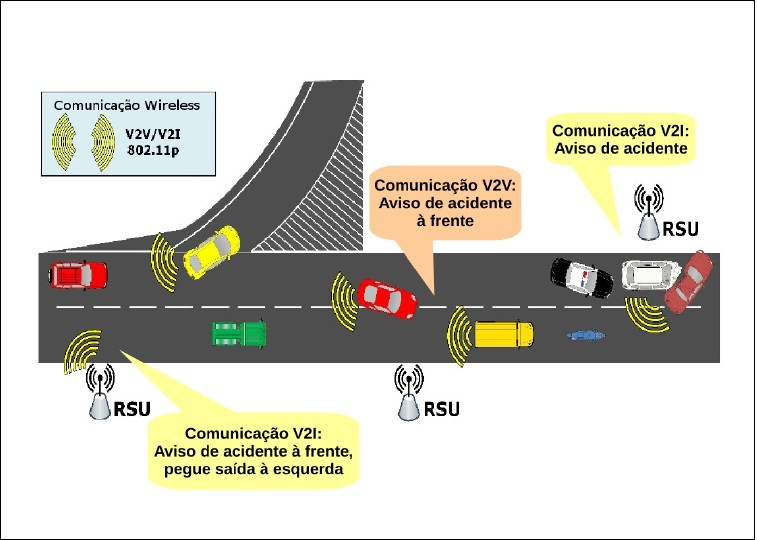
\includegraphics[scale=0.6]{imagens/vanet-comunicacao.jpg}}
  \caption[Shorter figure  caption]{Exemplo de funcionamento de  uma rede VANET.
(Fonte \cite{vehicular})} \label{fig:cen-vanet}
\end{figure}

A  maior diferença  entre  redes MANETs  e VANETs  está  no padrão  de
mobilidade dos nós, pois as VANETs apresentam uma mobilidade mais alta
e  seus  nós  realizam  movimentos pré  definidos  e  limitados  pelas
estradas.   O  principal  desafio  em  VANETs  consiste  em  manter  o
roteamento estável, uma vez que  as redes geradas pelas conexões entre
veículos são  muito dinâmicas  \cite{mustafa:2011}.  Segundo  Taleb et
al. \cite{taleb:2007},  tendo em vista  a alta mobilidade dos  nós, os
protocolos  de  roteamento  desenvolvidos  para  MANETs  precisam  ser
devidamente   adaptados  para   atender  efetivamente   um  roteamento
otimizado em VANETs.

Segundo  Peterson  et  al.    \cite{Peterson:2011},  em  uma  rede  de
comunicação existem  três métodos  fundamentais para a  transmissão de
dados: \textit{unicast},  \textit{broadcast} e  \textit{multicast}.  O
\textit{unicast}  é  a  forma  de  roteamento  onde  a  comunicação  é
realizada de um  para um, isto é, em cada  transmissão realizada um nó
age como origem e outro  como destino.  A abordagem \textit{broadcast}
realiza comunicação de um para todos, ou seja, um nó age como origem e
todos   os  outros   nós  da   rede  serão   destinos.   Por   fim,  o
\textit{multicast} realiza a comunicação de  um nó que age como origem
para  um   subconjunto  de   nós  que   são  destinos.    A  abordagem
\textit{multicast} é  o método  mais eficiente  para a  comunicação em
grupo, reduzindo  o desperdício  de recursos da  rede e  tornando mais
barato e  rápido o custo de  comunicação, uma vez que  as transmissões
para o conjunto  de nós destino são realizadas com  base em um caminho
lógico definido, sem obrigatoriedade  de replicação da informação para
todos os nós  da rede, independente deles estarem  interessados ou não
na mensagem, como acontece no {\em broadcast}. Uma desvantagem do {\em
  unicast} é  que o método gera  uma cópia da informação  para cada um
dos  nós  pelos  quais  o  pacote de  dados  deve  passar.   A  Figura
\ref{fig:metodos-transmissao}   ilustra   as    três   abordagens   de
transmissão.

\begin{figure}[!ht]
\fbox{
\begin{subfigure}{.3\textwidth}
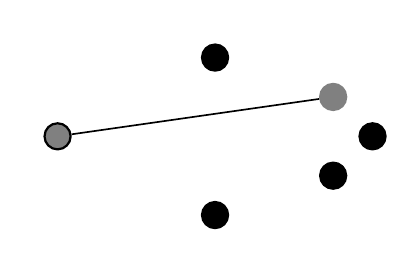
\begin{tikzpicture}[
            - = stealth, % arrow head style
            %shorten > = 0.7pt, % don't touch arrow head to node
            auto,
            node distance = 0.3cm, % distance between nodes
            semithick % line style
        ]

        \tikzstyle{every state}=[
            draw = black,
            thick,
            fill = black,
            minimum size = 3mm
        ]

        \node[state, fill = white, draw = white] (dummy) [at={(-1.7, 0.2)}] {};
        \node[state, fill = gray] (a) [at={(-1.5, -1)}]{};
        \node[state] (b) [at={(0.5, 0)}] {};
        \node[state] (c) [at={(0.5, -2)}] {};
        %\node[state, scale = 0.01] (d) [at={(-0.2, -1)}] {};
        \node[state, fill = gray, draw = gray] (e) [at={(2, -0.5)}] {};
        \node[state] (f) [at={(2, -1.5)}] {};
        \node[state] (g) [at={(2.5, -1)}] {};
        
        \path[-] (a) edge node {} (e);
        %\path[-] (d) edge node {} (e);        
    \end{tikzpicture}
\subcaption{\label{subfig:unicast} Unicast}
\end{subfigure}} \hfill
% Broadcast
\fbox{
\begin{subfigure}{.3\textwidth}
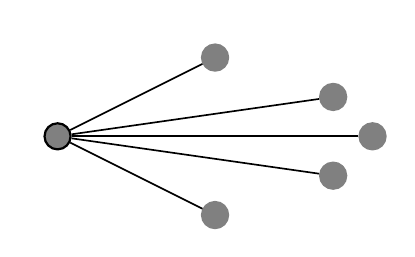
\begin{tikzpicture}[
            - = stealth, % arrow head style
            %shorten > = 0.7pt, % don't touch arrow head to node
            auto,
            node distance = 0.3cm, % distance between nodes
            semithick % line style
        ]

        \tikzstyle{every state}=[
            draw = gray,
            thick,
            fill = gray,
            minimum size = 3mm
        ]
        \node[state, fill = white, draw = white] (dummy) [at={(-1.7, 0.2)}] {};
        \node[state, draw = black] (d) [at={(-1.5, -1)}]{};
        \node[state] (b) [at={(0.5, 0)}] {};
        \node[state] (c) [at={(0.5, -2)}] {};
        %\node[state, scale = 0.01] (d) [at={(-0.2, -1)}] {};
        \node[state] (e) [at={(2, -0.5)}] {};
        \node[state] (f) [at={(2, -1.5)}] {};
        \node[state] (g) [at={(2.5, -1)}] {};
        
        %\path[-] (a) edge node {} (d);
        \path[-] (d) edge node {} (e);
        \path[-] (d) edge node {} (b);
        \path[-] (d) edge node {} (f);
        \path[-] (d) edge node {} (g);
        \path[-] (d) edge node {} (c);
        
    \end{tikzpicture}
\subcaption{\label{subfig:broadcast} Broadcast}
\end{subfigure}} \hfill
% Multicast
\fbox{
\begin{subfigure}{.3\textwidth}
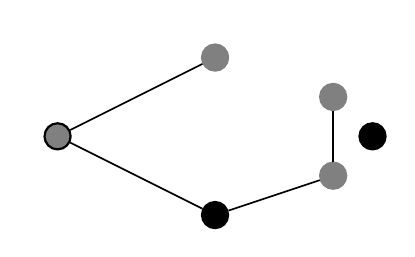
\begin{tikzpicture}[
            - = stealth, % arrow head style
            %shorten > = 0.7pt, % don't touch arrow head to node
            auto,
            node distance = 0.3cm, % distance between nodes
            semithick % line style
        ]

        \tikzstyle{every state}=[
            draw = gray,
            thick,
            fill = gray,
            minimum size = 3mm
        ]
        \node[state, fill = white, draw = white] (dummy) [at={(-1.7, 0.2)}] {};
        \node[state, draw = black] (d) [at={(-1.5, -1)}]{};
        \node[state] (b) [at={(0.5, 0)}] {};
        \node[state, draw = black, fill = black] (c) [at={(0.5, -2)}] {};
        %\node[state, scale = 0.01] (d) [at={(-0.2, -1)}] {};
        \node[state] (e) [at={(2, -0.5)}] {};
        \node[state] (f) [at={(2, -1.5)}] {};
        \node[state, draw = black, fill = black] (g) [at={(2.5, -1)}] {};
        
        %\path[-] (a) edge node {} (d);
        \path[-] (d) edge node {} (b);
        \path[-] (d) edge node {} (c);
        \path[-] (c) edge node {} (f);
        \path[-] (f) edge node {} (e);
        
    \end{tikzpicture}
\subcaption{\label{subfig:multicast} Multicast}
\end{subfigure}} \hfill
\caption{\label{fig:metodos-transmissao} Métodos usuais para transmissão de dados em redes}
\end{figure}

Em VANETs, assim como em outros  tipos de redes, as aplicações possuem
requisitos especiais em relação aos  recursos da rede.  A qualidade de
serviço, do inglês  \gls{qos}, está diretamente relacionada  com o uso
de demandas  de recursos da rede,  uma vez que em  muitas aplicações é
extremamente importante manter  o serviço da rede  com qualidade alta.
Por exemplo, aplicações relacionadas  à segurança, tais como mensagens
de  aviso de  colisão,  acidentes  ou más  condições  da estrada,  são
sensíveis ao atraso  na entrega das mensagens, bem  como aplicações de
multimídia  são  sensíveis à  largura  de  banda. Dentre  as  métricas
existentes, vale ressaltar algumas que são de extrema importância para
VANETs: atraso fim a fim (\textit{end-to-end delay}), \textit{jitter},
ou seja, variação  no atraso entre as mensagens para  o mesmo destino,
variação do  atraso fim  a fim entre  diferentes destinos,  largura de
banda (\textit{bandwidth}), quantidade de saltos da mensagem, ou seja,
a quantidade de nós pelos quais o  pacote passa até o destino final, e
estimativa de duração da conexão  entre veículos. Neste trabalho serão
consideradas as quatro primeiras  métricas citadas, explicadas em mais
detalhes a seguir.

Entende-se {\delay}  fim a fim como  o tempo gasto para  que um pacote
seja enviado da origem até o  destino.  O tempo total consiste na soma
dos atrasos do processamento nos nós  da rede e o atraso da propagação
ao longo  do meio de transmissão.   O \textit{jitter} é uma  medida da
variação do atraso na entrega entre sucessivos pacotes de dados em uma
conexão.  Para exemplificar, se um pacote enviado de uma origem até um
destino tem atraso  de 15 ms e  o envio de outro pacote  entre a mesma
origem  e destino  tem atraso  de 17  ms, isso  significa, de  maneira
simplificada, que o  {\jitter} dessa conexão é igual a  2 ms.  Segundo
Biradar e  Manvi \cite{biradar:2012},  é possível  reduzir o  valor do
{\jitter}  com  a  utilização de  \textit{buffers},  entretanto,  isso
aumenta consideravelmente a quantidade  de memória necessária, fazendo
com que seja preferível ter  o \textit{jitter} controlado pela própria
rede.

A variação  do {\delay}  entre os diferentes  destinos pode  ser definida
como a  diferença entre o atraso  do caminho que conecta  a origem com
qualquer  par de  destinos.  Limitar  essa variação  é essencial  para
sincronização  entre os  vários  receptores, garantindo  que não  haja
diferença de muitos  pacotes de uma mesma mensagem para  os vários nós
destinatários durante o tempo de vida de uma sessão \textit{multicast}
\cite{rouskas:1997}. Por  exemplo, assumindo um limite  de variação de
atraso entre diferentes destinos como 3 ms, se um pacote leva um tempo
de 17  ms para  ir da origem  para um destino,  um outro  destino deve
receber o  mesmo pacote com  o atraso no  intervalo de $[14,  20]$ ms.
Por fim, a largura de banda é a medida de capacidade de transmissão de
um determinado meio, conexão ou rede, determinando a velocidade máxima
em que os dados podem ser transmitidos no enlace.

De maneira mais informal, o problema de roteamento \textit{multicast},
do inglês \gls{mrp}, pode ser descrito  como um problema onde dados os
custos de transmissão de  mensagens entre veículos, busca-se minimizar
os  gastos  para  transferir  mensagens nó  raiz  até  um  determinado
subconjunto de  nós terminais.  Essa transmissão  pode utilizar outros
nós  da rede,  mas  não  precisa passar  por  todos eles.   Considerar
restrições de Qualidade  de Serviço, do inglês  \gls{qos}, trata-se de
garantir que  os caminhos percorridos  para realizar a  transmissão da
raiz para cada nó terminal  obedeçam às restrições de \gls{qos}. Essas
considerações resultam no \gls{mrp-qos}.

Uma propriedade essencial para garantir  que uma instância do \gls{mrp-qos} seja
viável é que exista pelo menos uma solução na qual todos os nós terminais possam
ser  atendidos.  Tipicamente  em  VANETs os  veículos  podem  ocasionalmente  se
desconectarem da  rede em  virtude de  suas elevadas  mobilidades, ou  seja, nem
sempre  é  possível garantir  que  todos  os  veículos  serão atendidos  a  todo
instante. Sendo assim, este trabalho propões uma nova variante do \gls{mrp-qos},
denominada  Máximo Atendimento  em  \gls{mrp} com  restrições  de \gls{qos},  do
inglês \gls{pma}, onde  nem todos os nós terminais da  rede podem ser atendidos.
Se o  caminho gerado  da raiz até  um terminal respeita  todas as  restrições de
\gls{qos}, esse terminal atendido, caso contrário,  o terminal não é atendido. O
objetivo do \gls{pma} é maximizar o serviço, i.e., atender o maior número de nós
terminais de acordo com as métricas de \gls{qos} impostas pela rede.

A Figura \ref{fig:ex1} apresenta um  exemplo do processo que constitui
a resolução  de uma  instância do  \gls{pma}. A  Figura \ref{subfig:a}
representa  o  grafo inicial,  tal  que  os nós  retangulares  (azuis)
representam  o conjunto  de veículos  terminais (destinos),  o nó  com
círculo  duplo (vermelho)  é o  nó raiz,  enquanto os  demais nós  são
opcionais.   Todas as  conexões  (links) tem  arcos bidirecionais,  ou
seja,  se  por exemplo  os  nós  1 e  4  estão  conectados é  possível
encaminhar mensagens na direção $(1, 4)$ e também $(4, 1)$.  Cada arco
contém 3 métricas associadas,  $\lambda$ ({\delay}), $\xi$ ({\jitter})
e  $\omega$ (largura  de  banda), uma  quarta  métrica utilizada  pelo
\gls{pma} é a de variação de  {\delay s} entre terminais.  No entanto,
ela não se aplica aos arcos individualmente  e sim a todos os pares de
caminhos   utilizados   para   atender   os   terminais.    A   Figura
\ref{subfig:b} apresenta uma solução  do \gls{pma}, onde foram gerados
caminhos, representados  pelos arcos ressaltados (azuis),  que atingem
todos  os  terminais. Nesse  caso  os  terminais com  retângulo  duplo
representam  veículos   atendidos  e   o  retângulo  simples   os  não
atendidos.  Nesse  exemplo,  dos  quatro terminais,  apenas  três  são
atendidos.

\begin{figure}[!ht]
\begin{subfigure}{.5\textwidth}
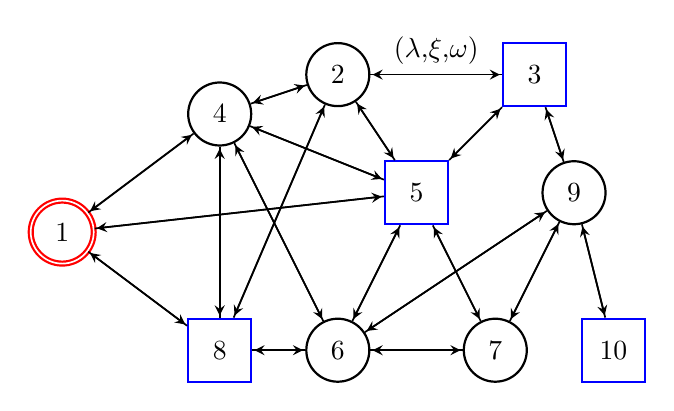
\begin{tikzpicture}[
            > = stealth, % arrow head style
            shorten > = 0.8pt, % don't touch arrow head to node
            auto,
            node distance = 1.5cm, % distance between nodes
            semithick % line style
        ]

        \tikzstyle{every state}=[
            draw = black,
            thick,
            fill = white,
            minimum size = 8mm
        ]

        \node[state, double, draw=red] (a) [at={(-1.5, -1)}]{$1$};
        \node[state] (b) [at={(2,1)}] {$2$};
        \node[state, rectangle, draw=blue] (c) [at={(4.5,1)}] {$3$};
        \node[state] (d) [at={(0.5, 0.5)}] {$4$};
        \node[state, rectangle, draw=blue] (e) [at={(3,-0.5)}] {$5$};
        \node[state] (f) [at={(2,-2.5)}] {$6$};
        \node[state] (g) [at={(4,-2.5)}] {$7$};
        %\node[state] (h) [at={(3,-2.5)}] {$6$};
        \node[state, rectangle, draw=blue] (i) [at={(0.5,-2.5)}] {$8$};
        \node[state] (j) [at={(5,-0.5)}] {$9$};
        \node[state, rectangle, draw=blue] (k) [at={(5.5,-2.5)}] {$10$};
        
        \path[->] (a) edge node {} (d); 
        \path[->] (d) edge node {} (a); 
        \path[->] (i) edge node {} (a);
        \path[->] (a) edge node {} (i);
        \path[->] (a) edge node {} (e);
        \path[->] (e) edge node {} (a);
        \path[->] (b) edge node {} (d);
        \path[->] (b) edge node {} (e);
        \path[->] (b) edge node {($\lambda$,$\xi$,$\omega$)} (c);
        \path[->] (c) edge node {} (e);
        \path[->] (e) edge node {} (f);
        \path[->] (d) edge node {} (i);
        \path[->] (d) edge node {} (e);
        \path[->] (d) edge node {} (f);
        \path[->] (e) edge node {} (g);
        \path[->] (f) edge node {} (j);
        \path[->] (c) edge node {} (j);
        \path[->] (i) edge node {} (f);
        \path[->] (i) edge node {} (b);
        \path[->] (j) edge node {} (k);
        \path[->] (j) edge node {} (g);
        \path[->] (d) edge node {} (b);
        \path[->] (e) edge node {} (b);
        \path[->] (c) edge node {} (b);
        \path[->] (e) edge node {} (c);
        \path[->] (f) edge node {} (e);
        \path[->] (f) edge node {} (g);
        \path[->] (g) edge node {} (f);
        \path[->] (i) edge node {} (d);
        \path[->] (e) edge node {} (d);
        \path[->] (f) edge node {} (d);
        \path[->] (g) edge node {} (e);
        \path[->] (j) edge node {} (f);
        \path[->] (j) edge node {} (c);
        \path[->] (f) edge node {} (i);
        \path[->] (b) edge node {} (i);
        \path[->] (k) edge node {} (j);
        \path[->] (g) edge node {} (j);
        
    \end{tikzpicture}
\subcaption{\label{subfig:a} Grafo com raiz e terminais}
\end{subfigure}
% Segunda figura
\begin{subfigure}{.5\textwidth}
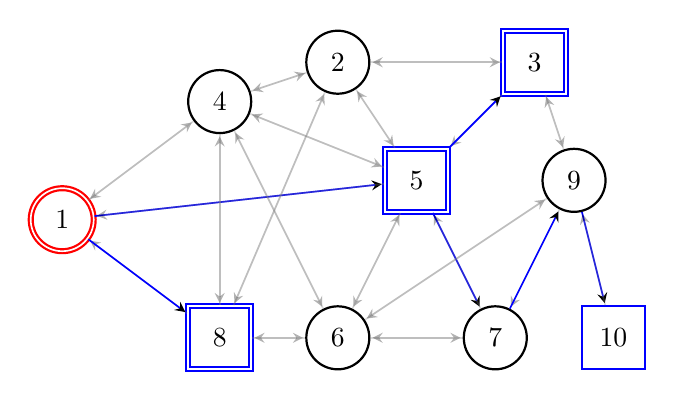
\begin{tikzpicture}[
            > = stealth, % arrow head style
            shorten > = 0.8pt, % don't touch arrow head to node
            auto,
            node distance = 1.5cm, % distance between nodes
            semithick % line style
        ]

        \tikzstyle{every state}=[
            draw = black,
            thick,
            fill = white,
            minimum size = 8mm
        ]

        \node[state, double, draw=red] (a) [at={(-1.5, -1)}]{$1$};
        \node[state] (b) [at={(2,1)}] {$2$};
        \node[state, double, rectangle, draw=blue] (c) [at={(4.5,1)}] {$3$};
        \node[state] (d) [at={(0.5, 0.5)}] {$4$};
        \node[state, double, rectangle, draw=blue] (e) [at={(3,-0.5)}] {$5$};
        \node[state] (f) [at={(2,-2.5)}] {$6$};
        \node[state] (g) [at={(4,-2.5)}] {$7$};
        %\node[state] (h) [at={(3,-2.5)}] {$6$};
        \node[state, double, rectangle, draw=blue] (i) [at={(0.5,-2.5)}] {$8$};
        \node[state] (j) [at={(5,-0.5)}] {$9$};
        \node[state, rectangle, draw=blue] (k) [at={(5.5,-2.5)}] {$10$};
        
        \path[->, draw = gray, opacity = 0.3] (a) edge node {} (d); 
        \path[->, draw = gray, opacity = 0.3] (d) edge node {} (a); 
        \path[->, draw = gray, opacity = 0.3] (i) edge node {} (a);
        \path[->, draw = blue] (a) edge node {} (i);
        \path[->, draw = blue] (a) edge node {} (e);
        \path[->, draw = gray, opacity = 0.3] (e) edge node {} (a);
        \path[->, draw = gray, opacity = 0.3] (b) edge node {} (d);
        \path[->, draw = gray, opacity = 0.3] (b) edge node {} (e);
        \path[->, draw = gray, opacity = 0.3] (b) edge node {} (c);
        \path[->, draw = gray, opacity = 0.3] (c) edge node {} (e);
        \path[->, draw = gray, opacity = 0.3] (e) edge node {} (f);
        \path[->, draw = gray, opacity = 0.3] (d) edge node {} (i);
        \path[->, draw = gray, opacity = 0.3] (d) edge node {} (e);
        \path[->, draw = gray, opacity = 0.3] (d) edge node {} (f);
        \path[->, draw = blue] (e) edge node {} (g);
        \path[->, draw = gray, opacity = 0.3] (f) edge node {} (j);
        \path[->, draw = gray, opacity = 0.3] (c) edge node {} (j);
        \path[->, draw = gray, opacity = 0.3] (i) edge node {} (f);
        \path[->, draw = gray, opacity = 0.3] (i) edge node {} (b);
        \path[->, draw = blue] (j) edge node {} (k);
        \path[->, draw = gray, opacity = 0.3] (j) edge node {} (g);
        \path[->, draw = gray, opacity = 0.3] (d) edge node {} (b);
        \path[->, draw = gray, opacity = 0.3] (e) edge node {} (b);
        \path[->, draw = gray, opacity = 0.3] (c) edge node {} (b);
        \path[->, draw = blue] (e) edge node {} (c);
        \path[->, draw = gray, opacity = 0.3] (f) edge node {} (e);
        \path[->, draw = gray, opacity = 0.3] (f) edge node {} (g);
        \path[->, draw = gray, opacity = 0.3] (g) edge node {} (f);
        \path[->, draw = gray, opacity = 0.3] (i) edge node {} (d);
        \path[->, draw = gray, opacity = 0.3] (e) edge node {} (d);
        \path[->, draw = gray, opacity = 0.3] (f) edge node {} (d);
        \path[->, draw = gray, opacity = 0.3] (g) edge node {} (e);
        \path[->, draw = gray, opacity = 0.3] (j) edge node {} (f);
        \path[->, draw = gray, opacity = 0.3] (j) edge node {} (c);
        \path[->, draw = gray, opacity = 0.3] (f) edge node {} (i);
        \path[->, draw = gray, opacity = 0.3] (b) edge node {} (i);
        \path[->, draw = gray, opacity = 0.3] (k) edge node {} (j);
        \path[->, draw = blue] (g) edge node {} (j);
    \end{tikzpicture}
\subcaption{\label{subfig:b} Caminho da mensagem}
\end{subfigure}
\caption{\label{fig:ex1} Exemplo de Instância do MS-MRP-QoS}
\end{figure}

Neste trabalho investigamos o \gls{pma} visando encontrar metodologias
eficazes para  resolvê-lo.  Para alcançar esse  objetivo, inicialmente
resolvemos  o  \gls{pma}  de   maneira  exata  utilizando  \gls{plim}.
Desenvolvemos  um  conjunto  de quatro  relaxações  lagrangianas  para
obtenção de limitantes inferiores e  superiores com base na dualização
de  restrições complicadoras.   Por fim,  foram desenvolvidos  métodos
heurísticos para obter  soluções sem garantia de  otimalidade, mas com
um  baixo uso  de recursos  computacionais.  Uma  heurística de  busca
local  em  arborescências  foi  aplicada   com  objetivo  de  gerar  e
aperfeiçoar soluções viáveis em conjunto  com a solução das relaxações
lagrangianas.   Também foram  propostos três  Algoritmos Genéticos  de
Chaves Aleatórias Viciadas, do  inglês \gls{brkga}, contendo variações
no decodificador, no  cálculo da função objetivo e  no procedimento de
geração das chaves aleatórias.  Por fim, as instâncias utilizadas para
os experimentos foram  geradas utilizando simuladores de  tráfego e de
rede.

Esta  dissertação  está  organizada  em seis  capítulos.   O  Capítulo
\eqref{chp:preliminares}  introduz notações  e definições  necessárias
para o  entendimento dos demais  capítulos, incluindo a  descrição dos
modelos de \gls{pli} e \gls{plim}, e as principais técnicas utilizadas
neste   trabalho   são  descritas   de   modo   geral.   No   Capítulo
\ref{chp:trab-relacionados},  as principais  publicações presentes  na
literatura  para  problemas  de  otimização em  redes  veiculares  são
apresentadas,   com  foco   nos  resultados   obtidos.   No   Capítulo
\ref{chapter:metodologia}, são  discutidas as  metodologias utilizadas
no  desenvolvimento deste  trabalho.  A  descrição dos  experimentos e
resultados  computacionais é  feita no  Capítulo \ref{chp:resultados}.
Por   fim,   o   Capítulo   \ref{chp:consideracoes-finais}   traz   as
considerações finais do trabalho, seguido das referências.


\chapter{Conceitos Preliminares e Formulações do Problema} \label{chp:preliminares}

Neste capítulo introduzimos conceitos fundamentais para o entendimento
desta dissertação.  Notações e  definições básicas são apresentadas na
Seção  \ref{sec:not-e-def}.   Neste   trabalho,  empregamos  conceitos
básicos  de  Otimização  Combinatória,  os  quais  assume-se  que  são
conhecidos. Caso o leitor  julgue necessária uma revisão, recomendamos
o livro texto de Nemhauser e Wolsey \cite{Nemhauser}, o qual cobre tal
tema  com  enfoque  em   \gls{pli},  uma  das  principais  ferramentas
utilizadas neste trabalho.  Os conceitos básicos relacionados à teoria
dos  grafos  são  considerados  conhecidos  e  caso  o  leitor  julgue
necessário uma revisão  o conteúdo pode ser encontrado  em algum livro
texto  sobre o  tema,  por exemplo,  Diestel \cite{diestel:2005}.   Os
modelos  matemáticos estão  contidos nas  Seções \ref{sec:dmfm-pma}  e
\ref{sec:ab-pma}.   A   Seção  \ref{sec:rel-lagrangiana}   contém  uma
descrição do  funcionamento e aplicação da  relaxação lagrangiana, uma
das  principais abordagens  por nós  utilizada.  Por  fim, nas  Seções
\ref{sec:metaheuristic}  e  \ref{subsec:brkga}  discutimos,  de  forma
geral, meta-heurísticas e \gls{brkga}.

\section{Notações e Definições} \label{sec:not-e-def}

Seja um grafo  ponderado e direcionado $G  = (V, A)$, sendo  $V = \{1,
\dots, n\}$ seu conjunto  de vértices, $A = \{(u, v) : u  \text{ e } v
\in V, u \neq v\}$ seu conjunto  de $m$ arcos, onde o primeiro vértice
do  arco é  a fonte  e também  predecessor do  segundo vértice  do par
ordenado, que  é conhecido  como destino.   Tratando-se de  grafos não
direcionados, podemos  substituir a nomenclatura do  conjunto de arcos
$A$ pelo conjunto  de arestas $E$. Uma árvore $T$,  obtida a partir de
um grafo  não orientado  $G$, é um  subgrafo de $G$  conexo e  que não
contém  ciclos. Para  que  $T$  seja geradora  em  $G$  o conjunto  de
vértices $V(T)$ deve ser igual a $V(G)$, ou seja, todos os vértices do
grafo fazem parte da árvore. Uma arborescência, ou árvore enraizada, é
um grafo direcionado  no qual exatamente um vértice,  digamos $s$, tem
grau de  entrada $0$ e  nenhum vértice tem  grau de entrada  maior que
$1$, de modo  que todos os vértices do grafo  são alcançáveis a partir
da raiz $s$.

Segue  uma  definição  formal  do  \gls{pma}.   Seja  uma  rede  VANET
representada como  um grafo direcionado  ponderado $G = (V,  A)$. Cada
arco de  $G$ contém três  métricas de \gls{qos} associadas:  {\delay ,
  \jitter} e largura  de banda.  Definimos a entrada  o \gls{pma} como
uma  tupla  ($G(V,  A),  \lambda,   \xi,  \omega,  s,  D,  \Delta_{d},
\Delta_{j}, \Delta_{v}, \Phi$), onde:

\begin{itemize}
    \item $G = (V, A)$ é um grafo ponderado orientado;
    \item $\lambda_{ij} :  A \rightarrow \mathbb{N}$ é  uma função que
      retorna o valor de \textit{delay} para cada arco $(i, j) \in A$;
    \item  $\xi_{ij} :  A  \rightarrow \mathbb{N}$  é  uma função  que
      retorna o  valor de \textit{jitter}  para cada arco $(i,  j) \in
      A$;
    \item $\omega_{ij}  : A \rightarrow  \mathbb{N}$ é uma  função que
      retorna o valor  de largura de banda para cada  arco $(i, j) \in
      A$;
    \item $s \in V$ é definido como a raiz;
    \item $D$ é o conjunto de vértices terminais, tal que $D \subseteq
      (V \backslash \{s\}$);
    \item  $\Delta_{d}$  é  uma  constante  que  indica  o  limite  de
      \textit{delay} fim a fim permitido no caminho de $s$ até cada um
      dos vértices de $D$;
    \item  $\Delta_{j}$  é  uma  constante  que  indica  o  limite  de
      \textit{jitter}  permitido no  caminho de  $s$ até  cada um  dos
      vértices de $D$;
    \item $\Delta_{v}$ é uma constante que indica o limite da variação
      dos atrasos  fim a fim entre  todos os pares de  caminhos de $s$
      até algum vértice de $D$;
    \item $\Phi$  é uma constante  que indica  o mínimo de  largura de
      banda necessário para que um  arco qualquer possa fazer parte da
      solução;
\end{itemize}

O conjunto $S \in V \backslash (D \cup \{s\})$ é composto por todos os
vértices  restantes de  $V$. Assim,  os vértices  do conjunto  $S$ são
chamados de  opcionais ou  de \textit{Steiner}. Vale  também ressaltar
que,   como  as   conexões  para   comunicação  da   rede  VANET   são
bidirecionais, se  o arco $(i, j)$  pertence a $A$, então  o arco $(j,
i)$   também  está   contido  em   $A$  com   os  mesmos   valores  de
\gls{qos}. Quando a largura de banda $\omega$ de um arco $(i, j)$ está
com  o valor  abaixo do  limite demandado  pela \gls{qos}  ($\Phi$), o
mesmo não é adicionado ao conjunto $A$ e, consequentemente, nunca será
parte  de   uma  solução  viável  do   \gls{pma}.   Uma  arborescência
\textit{multicast} $T$ de  $G$ tem o vértice fonte $s$  como sua raiz,
alcança todos  os vértices terminais  em $D$ e,  possivelmente, alguns
vértices de $S$, mas não necessariamente todos.

O grafo descrito acima permite  uma modelagem correta do problema, mas
é  possível garantir  que qualquer  solução viável  corresponda a  uma
arborescência geradora. Isso é  conveniente pois formulações fortes de
programação  inteira  para  arborescências  geradoras  são  conhecidas
\cite{MAGNANTI1995503}.   As seguintes  mudanças  foram realizadas  no
grafo  para  garantir  a  existência  de  uma  solução  que  seja  uma
arborescência geradora:

\begin{enumerate}
    \item  Adiciona-se  um vértice  artificial  $s'$  e um  novo  arco
      artificial  de  $s$ para  $s'$  cujo  \textit{delay} é  igual  a
      $\Delta_d + 1$ e \textit{jitter} igual a $\Delta_j + 1$.
    \item São  adicionados arcos de  $s'$ para  cada vértice $k  \in D
      \cup S$ com \textit{delay} e \textit{jitter} iguais a 0.
\end{enumerate}


O grafo resultante é $G' = (V', A')$,  onde $V' = V \cup \{s'\}$ e $A'
= A \cup \{(s, s')\} \cup \{(s', k) : k \in D \cup S\}$. Como foi dito
anteriormente,   soluções   viáveis   nesse  grafo   são   dadas   por
arborescências  geradoras  na  qual  $s$  é  a  raiz.   Contudo,  para
representar  adequadamente  soluções   factíveis,  algumas  restrições
precisam ser acrescentadas.   A arborescência deve conter  o arco $(s,
s')$ e  se o caminho  de $s$ até qualquer  terminal $k$ utilizar  o nó
$s'$ como intermediário, então $k$  não é atendido. O propósito dessas
restrições é fazer com que haja uma  subárvore onde $s'$ é a raiz e os
nós  opcionais que  não foram  utilizados como  encaminhadores ou  nós
terminais não atendidos sejam visitados pela arborescência a partir de
$s'$.

Utilizando como exemplo  o grafo $G$ e a  arborescência apresentada na
Figura  \ref{fig:ex1}  do  capítulo anterior,  serão  ilustradas  duas
possíveis  soluções  viáveis  com  base  em  $G$  e  $G'$.   A  Figura
\ref{fig:arb-ex1} descreve uma solução viável  obtida a partir de $G$,
enquanto  a Figura  \ref{fig:arb-ex2} apresenta  uma arborescência  na
qual o  mesmo número de  terminais é  atendido mas a  representação da
solução  é  uma  arborescência  geradora  que utiliza  o  nó  e  arcos
artificiais.

\begin{figure}[!ht]
  \begin{subfigure}{.5\textwidth}
  \centering
  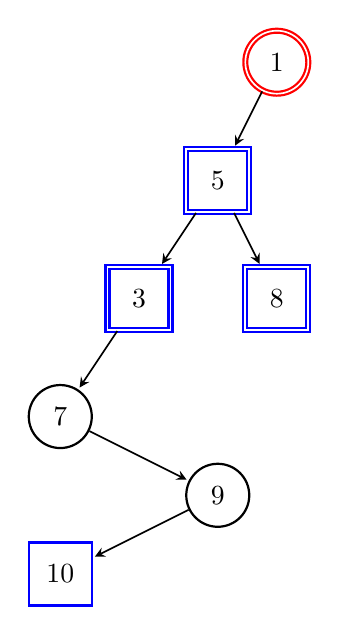
\begin{tikzpicture}[
      > = stealth, % arrow head style
      shorten > = 0.8pt, % don't touch arrow head to node
      auto,
      node distance = 1.5cm, % distance between nodes
      semithick, % line style
    ]

    \tikzstyle{every state}=[
      draw = black,
      thick,
      fill = white,
      minimum size = 8mm
    ]
    
    \node[state, double, draw = red] (a) [at={(5, 2.5)}]{$1$};
    \node[state, double, rectangle, draw = blue] (e) [at={(4.25, 1)}] {$5$};
    \node[state, double, rectangle, draw = blue] (h) [at={(5, -0.5)}] {$8$};
    \node[state, double, rectangle, draw = blue] (c) [at={(3.25, -0.5)}] {$3$};
    \node[state] (g) [at={(2.25, -2)}] {$7$};
    \node[state] (i) [at={(4.25, -3)}] {$9$};
    \node[state, rectangle, draw = blue] (j) [at={(2.25, -4)}] {$10$};

    \path[->] (a) edge node {} (e); 
    \path[->] (e) edge node {} (c);
    \path[->] (e) edge node {} (h);
    \path[->] (c) edge node {} (g);
    \path[->] (g) edge node {} (i);
    \path[->] (i) edge node {} (j);

  \end{tikzpicture}
  \subcaption{\label{fig:arb-ex1} Arborescência obtida a partir de G}
  \end{subfigure}
  \begin{subfigure}{.5\textwidth}
      \centering
  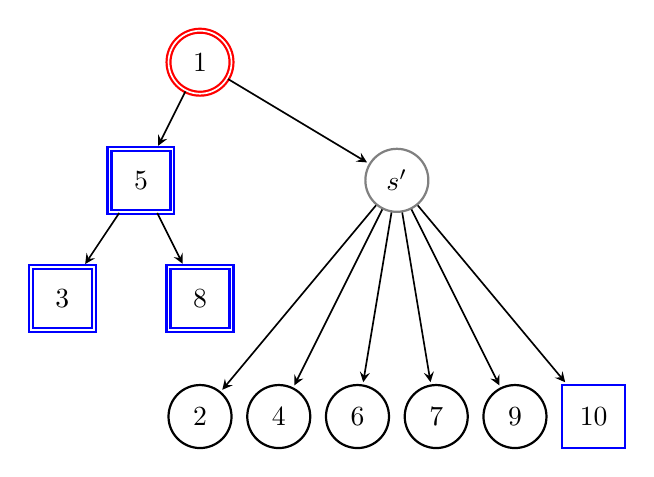
\begin{tikzpicture}[
      > = stealth, % arrow head style
      shorten > = 0.8pt, % don't touch arrow head to node
      auto,
      node distance = 1.5cm, % distance between nodes
      semithick, % line style
    ]

    \tikzstyle{every state}=[
      draw = black,
      thick,
      fill = white,
      minimum size = 8mm
    ]
    
    \node[state, double, draw = red] (a) [at={(5, 2.5)}]{$1$};
    \node[state, double, rectangle, draw = blue] (e) [at={(4.25, 1)}] {$5$};
    \node[state, draw = gray] (z) [at={(7.5, 1)}] {$s'$};
    \node[state, double, rectangle, draw = blue] (h) [at={(5, -0.5)}] {$8$};
    \node[state, double, rectangle, draw = blue] (c) [at={(3.25, -0.5)}] {$3$};
    \node[state] (g) [at={(8, -2)}] {$7$};
    \node[state] (i) [at={(9, -2)}] {$9$};
    \node[state, rectangle, draw = blue] (j) [at={(10, -2)}] {$10$};
    \node[state] (b) [at={(5, -2)}] {$2$};
    \node[state] (d) [at={(6, -2)}] {$4$};
    \node[state] (f) [at={(7, -2)}] {$6$};
%    \node[state] (j) [at={(7.5,-2)}] {$8$};
%    \node[state] (k) [at={(8.4,-2)}] {$9$};
%    \node[state] (l) [at={(9.3,-2)}] {$10$};
%    
    \path[->] (a) edge node {} (e); 
    \path[->] (e) edge node {} (c);
    \path[->] (e) edge node {} (h);
    \path[->] (z) edge node {} (g);
    \path[->] (z) edge node {} (i);
    \path[->] (z) edge node {} (j);
    \path[->] (z) edge node {} (b);
    \path[->] (z) edge node {} (d);
    \path[->] (z) edge node {} (f);
    \path[->] (a) edge node {} (z);    
  \end{tikzpicture}
  \vspace*{2cm}
  \subcaption{\label{fig:arb-ex2} Arborescência obtida a partir de G'}
  \end{subfigure}
\end{figure}

Com base  na adaptação para  garantir que toda solução  é representada
por  uma  arborescência  geradora,  desenvolvemos  uma  formulação  de
\gls{pli}  para  o  \gls{pma},  baseada na  formulação  de  multifluxo
apresentada por Magnanti e  Wolsey \cite{MAGNANTI1995503}, a qual será
denotada no restante deste  documento por \gls{dmfm-pma}, um mnemônico
do inglês {\em \textbf{D}irected \textbf{M}ulticommodity \textbf{F}low
  \textbf{M}odel}  - MRP.   A segunda  modelagem desenvolvida  utiliza
programação inteira mista,  ou seja, utiliza-se de  variáveis reais em
conjunto com as variáveis inteiras.  Esse segundo modelo foi elaborado
com base  na remoção das variáveis  de fluxo do \gls{dmfm-pma}  e será
denotada no  restante do documento  por \gls{ab-pma}, um  mnemônico do
inglês {\em \textbf{A}rborescence \textbf{B}ased} - MRP.

\section{Modelo de PLI DMFM-MRP} \label{sec:dmfm-pma}

Dada uma instância  $I_{MS-MRP-QoS} = (G(V, A),  \lambda, \xi, \omega,
s,  D, \Delta_{d},  \Delta_{j}, \Delta_{v},  \Phi)$ para  o \gls{pma},
considere as seguintes variáveis:

\begin{itemize}
 \item $f_{ij}^{k}$: Uma variável binária indicando se o arco $(i, j)$
   pertence ao caminho da fonte $s$ até o vértice $k$ tal que $k \in D
   \cup S$,  alternativamente, se o fluxo  de $s$ para $k$  passa pelo
   arco $(i, j)$;
 \item $y_{ij}$: Uma  variável binária que recebe valor 1  caso o arco
   $(i, j)$ pertença a arborescência ótima e 0 caso contrário;
 \item $z_{k}$: Uma variável binária que  recebe valor 1 se o terminal
   $k$ não é atendido e 0 caso contrário.
\end{itemize}

Assim, um modelo de programação inteira para o \gls{pma} é:

\allowdisplaybreaks
%%%%%%%%%%%%%%%%%%%%%%%%%%%%%%%%%%%%%%%%%%%%%%%%%%%%%%%%%%%%%%%%%%%%%%
\begin{align}
\text{(IP)} \quad 
    & \displaystyle \min \sum_{k \in D}z_k & \label{eq:mod-fo} \\
\text{s.a.:} \quad
    & \displaystyle \sum_{(s, j) \in A'} f_{sj}^{k} - \sum_{(j, s) \in A'} f_{js}^{k} = 1 & \forall k \in D \label{eq:fluxo-raiz} \\
    & \displaystyle \sum_{(i, j) \in A'} f_{ij}^{k} - \sum_{(j, i) \in A'} f_{ji}^{k} = 0 & \forall j \in V \backslash \{s, k\}, \forall k \in D \cup S \label{eq:fluxo-qualquer} \\
    & \displaystyle \sum_{(k, j) \in A'} f_{kj}^{k} - \sum_{(j, k) \in A'} f_{jk}^{k} = -1 & \forall k \in D \cup S \label{eq:fluxo-terminal} \\
    & f_{ij}^{k} \leq  y_{ij} & \forall (i, j) \in A', \forall k \in D \cup S \label{eq:rel-f-y-term} \\
    & \displaystyle \sum_{(i, j) \in A'} y_{ij} = |V| & \label{eq:num-arestas-arvore} \\
    & \displaystyle \sum_{(i, j) \in A'} \lambda_{ij}f_{ij}^{k} \leq  \Delta_{d} + M_dz_k
     & \forall k \in D \label{eq:mod-lim-delay} \\
%- modificada --------------------------------------------------------
    & \displaystyle \sum_{(i, j) \in A'} \xi_{ij}f_{ij}^{k} \leq  \Delta_{j} + M_jz_k
     & \forall k \in D \label{eq:mod-lim-jitter} \\
%- modificada --------------------------------------------------------
    & \displaystyle \sum_{(i, j) \in A'} \lambda_{ij}(f_{ij}^{k} - f_{ij}^{l}) \leq \Delta_{v} 
       + M_v^kz_k + M_v^lz_l 
    & \forall k, l \in D, k \neq l \label{eq:mod-var-delay} \\
    %& z_k \geq f_{ss'}^{k} & \forall k \in D \label{eq:fluxo-terminal-dummy-node} \\
    %& f_{s'q}^{e} = 0  & \forall q \in D \cup S, \forall e \in D \cup S \backslash\{q\} \label{eq:steiner-leaf} \\
    & y_{ss'} = 1 & \label{eq:force-dummy-node} \\
%---------------------------------------------------------------------
    & f_{ij}^{k} \in \{0, 1\} & \forall (i, j) \in A', \forall k \in D \cup S \label{eq:dom-f} \\
    &  y_{ij} \in \{0, 1\} &  \forall (i, j) \in A' \label{eq:dom-y} \\
    &  z_{i} \in \{0, 1\} &  \forall i \in D \label{eq:dom-z} 
\end{align}

O  modelo  \gls{dmfm-pma}  apresenta como  solução  uma  arborescência
conectando  a  raiz a  todos  os  nós  terminais.  A  função  objetivo
\eqref{eq:mod-fo} minimiza  o número  de terminais não  atendidos.  As
restrições  \eqref{eq:fluxo-raiz}-\eqref{eq:fluxo-terminal}  impõem  a
conservação de  fluxo em cada  vértice, forçando ainda que  apenas uma
unidade de fluxo  saia da fonte $s$  para cada destino $K  \in D$.  As
restrições  \eqref{eq:rel-f-y-term}   garantem  que  não   haja  fluxo
passando por  um arco $(i,  j)$ e dirigindo-se a  um vértice $k  \in D
\cup S$,  a menos  que esse  arco pertença  à arborescência  ótima.  A
restrição \eqref{eq:num-arestas-arvore} força que a solução tenha $|V|
= |D| + |S| + 1$ arcos,  portanto, gera todos os vértices de $G'$.  As
restrições \eqref{eq:mod-lim-delay}-\eqref{eq:mod-lim-jitter} limitam,
respectivamente,  o delay  e o  jitter no  caminho para  cada terminal
atendido.   As   restrições  \eqref{eq:mod-var-delay}  exigem   que  a
diferença entre os \textit{delays} de  quaisquer dois caminhos que vão
de $s$ até um  terminal $k \in D$ não seja  maior que $\Delta_v$, caso
ambos     os    terminais     sejam     atendidos.     A     restrição
\eqref{eq:force-dummy-node} garante que o arco $(s, s')$ faça parte da
solução final,  evitando a ocorrência  de ciclos com  a característica
$y_{ij}    =    y_{ji}    =    1$.     Finalmente,    as    restrições
\eqref{eq:dom-f}-\eqref{eq:dom-z} definem os domínios das variáveis.

É  necessário  ainda  uma  descrição  mais  detalhada  das  restrições
(\ref{eq:mod-lim-delay}),          (\ref{eq:mod-lim-jitter})         e
(\ref{eq:mod-var-delay}).   As  duas  primeiras  restrições  tornam-se
inativas quando o  terminal ao qual elas se referem  não for atendido,
enquanto a última restrição torna-se  inativa quando pelo menos um dos
terminais  ao qual  ela se  refere não  for atendido.   Para isso,  os
parâmetros  $M_d$,  $M_j$,  $M_v^k$  e $M_v^l$  devem  ser  escolhidos
convenientemente de  modo a  manter as restrições  válidas.  Possíveis
valores para esses parâmetros serão discutidos posteriormente.

\section{Modelo de Programação Inteira Mista - AB-MRP} \label{sec:ab-pma}

Dada uma  instância $I_{PMA} = (G(V,  A), \lambda, \xi, \omega,  s, D,
\Delta_{d}, \Delta_{j}, \Delta_{v}, \Phi)$ para o \gls{pma}, considere
as seguintes variáveis:

\begin{itemize}
 \item $y_{ij}$: Uma  variável binária que recebe valor 1  caso o arco
   $(i, j)$ pertença à arborescência ótima e 0 caso contrário;
 \item $z_{k}$: Uma variável binária que  recebe valor 1 se o terminal
   $k$ não é atendido e 0 caso contrário;
 \item $a_{i}$: Uma  variável real que representa  o \textit{delay} do
   caminho de $s$ até $i$, caso $i$ faça parte da arborescência ótima;
 \item $t_{i}$: Uma variável real  que representa o \textit{jitter} do
   caminho de $s$ até $i$, caso $i$ faça parte da arborescência ótima;
\end{itemize}

Assim, o  modelo de  programação linear  inteira mista  \gls{ab-pma} é
proposto a seguir:

\begin{align}
 & \text{(MIP)} \min \sum_{k \in D} z_k & \label{eq:ab-fo} \\ 
 & \sum_{(i, j) \in A'} y_{ij} = 1 & \forall j \in D \cup S \label{eq:spanning} \\
 %& \sum_{(i, j) \in A^{-}(S)} y_{ij} \geq 1 & \forall S \in V\backslash \{s\} \label{eq:desigualdade-opicional}\\
 & a_j \geq a_i + \lambda_{ij} y_{ij} - M_d(1 - y_{ij}) & \forall (i, j) \in A' \label{eq:lambda-geq} \\
 & a_j \leq a_i + \lambda_{ij} y_{ij} + M_d(1 - y_{ij}) & \forall (i, j) \in A' \label{eq:lambda-leq} \\
 & t_j \geq t_i + \xi_{ij} y_{ij} - M_j(1 - y_{ij})& \forall (i, j) \in A' \label{eq:xi-geq} \\
 %& t_j \leq t_i + \xi_{ij} y_{ij} + M_j(1 - y_{ij})& \forall (i, j) \in A' \label{eq:xi-leq} \\
 & a_k \leq \Delta_d + M_d z_k & \forall k \in D \label{eq:lim-delay} \\
 & t_k \leq \Delta_j + M_j z_k & \forall k \in D \label{eq:lim-jitter} \\
 & a_k - a_l \leq \Delta_v + M_v^k z_k + M_v^l z_l & \forall k, l \in D, k \neq l \label{eq:lim-var} \\
 %& y_{ss'} = 1 & \label{eq:ab-force-art-vert} \\
 & y_{ij} \in \{0, 1\} & \forall (i, j) \in A' \label{eq:ab-dom-y} \\
 & z_{k} \in \{0, 1\} & \forall k \in D \label{eq:ab-dom-z}\\
 & a_i, t_i \geq 0 & \forall i \in V \label{eq:ab-dom-l-t} 
\end{align}

No  modelo  \gls{ab-pma}  uma  solução  representa  uma  arborescência
geradora  mínima onde  os valores  das métricas  de \gls{qos}  de cada
caminho são  calculadas nos  nós.  A função  objetivo \eqref{eq:ab-fo}
minimiza  o   número  de  terminais  não   atendidos.   As  restrições
\eqref{eq:spanning}  garantem  que  a arborescência  é  geradora.   As
restrições   \eqref{eq:lambda-geq}-\eqref{eq:lambda-leq}  calculam   o
custo de  \textit{delay} em cada vértice  $j$, de modo que,  se o arco
$(i, j)$ pertencer  a arborescência ótima, o valor de  $a_j$ é igual a
$a_i + \lambda_{ij}$. As  restrições \eqref{eq:xi-geq} aplicam o mesmo
princípio  das  restrições  \eqref{eq:lambda-geq} sobre  as  variáveis
$t_i$. Para a variável  $a_k$, o delay em um nó $k \in  D \cup S$ será
exatamente  o  {\delay} acumulado  no  caminho  até  $k$. No  caso  da
variável $t_k$, é  suficiente que ela seja maior ou  igual ao valor de
{\jitter}  acumulado, pois  ao contrário  do {\delay}  não existe  uma
restrição  limitando a  variação de  {\jitter}. Cabe  observar que  os
valores  computados   para  as   variáveis  $l_k$  e   $t_k$  dependem
diretamente  dos valores  das mesmas  variáveis no  nó predecessor  de
$k$. Essa dependência impede a formação de ciclos na solução ótima. As
restrições       \eqref{eq:lim-delay}-\eqref{eq:lim-var}       limitam
respectivamente \textit{delay}, \textit{jitter} e variação de {\delay}
utilizando      a       mesma      abordagem       das      restrições
\eqref{eq:mod-lim-delay}-\eqref{eq:mod-var-delay}       do      modelo
\gls{dmfm-pma}.          Por         fim,        as         restrições
\eqref{eq:ab-dom-y}-\eqref{eq:ab-dom-l-t}  definem   os  domínios  das
variáveis.

\subsection{Possíveis valores para os parâmetros $M$} \label{subsec:m-param}

A  seguir discutiremos  sobre possíveis  valores das  constantes $M_d,
M_j, M^k_v$ e $M^l_v$. Foram propostos valores que podem ser aplicados
à modelagem  considerando o  grafo $G$  sem a adição  dos nós  e arcos
artificiais.  Também foram propostos  valores que podem ser utilizados
apenas para o grafo for $G'$.

Inicialmente, suponha  que os  arcos do grafo  $G=(V, A)$  tenham sido
indexadas de  1 a $m  = |A|$,  ou seja, $A  = \{e_1,e_2,\ldots,e_m\}$.
Suponha também que $\lambda_{e_1}  \geq \lambda_{e_2} \geq \ldots \geq
\lambda_{e_m}$. Agora, para $n=|V|$, qualquer caminho simples no grafo
tem  no  máximo  $n-1$ arcos  e,  portanto,  $\Lambda=\sum_{i=1}^{n-1}
\lambda_{e_i}$ é um limitante superior  para o \textit{delay} total de
qualquer  caminho no  grafo.   De forma  análoga,  pode-se definir  um
limitante superior para o  \textit{jitter} de qualquer caminho simples
de $G$, o  qual será denotado por $\Xi$.  Também  será usada a notação
$SP_\lambda(k)$ para o  comprimento do caminho mais curto  da raiz $s$
para o vértice $k$ de $G$ utilizando como métrica o \textit{delay}.

Com  as definições  do  parágrafo anterior,  pode-se computar  valores
viáveis para as constantes $M_d$, $M_j$, $M_v^k$ e $M_v^l$ da seguinte
forma:

\begin{align}
  M_d = & \quad \Lambda-\Delta_d & \label{it:delay} \\
  M_j = & \quad \Xi-\Delta_j & \label{it:jitter} \\
  M_v^k = & \quad \Lambda-\mu, \text{ onde } \mu=\min\{\text{SP}_\lambda(l)+\Delta_v,\Delta_d\} & \label{it:vardelay-k}\\
  M_v^l = & \quad \Delta_d - \Delta_v - \text{SP}_\lambda(l) & \label{it:vardelay-l}
\end{align}

Considerando  as  definições de  $\Lambda$  e  $\Xi$ e  analisando  as
restrições (\ref{eq:mod-lim-delay}) e (\ref{eq:mod-lim-jitter}), temos
que se o terminal $k$ for  atendido ($z_k = 0$), essas duas restrições
limitam o {\delay} e o  {\jitter} conforme determinado pela \gls{qos}.
Por outro lado,  se $k$ não for  atendido ($z_k = 1$), o  {\delay} e o
{\jitter} acumulado no caminho de $s$  a $k$ ficam restritos de acordo
com  os seus  limitantes superiores  $\Lambda$ e  $\Xi$ subtraídos  do
valor  máximo de  acumulado para  que $k$  seja atendido,  usando como
métricas o {\delay} e o {\jitter}, respectivamente.

A restrição (\ref{eq:mod-var-delay}), que  controla a variação de {\em
  delay}, requer uma análise mais aprofundada.  O objetivo é encontrar
um  limitante superior  para o  lado direito  da restrição  nas quatro
situações  possíveis de  atendimento  do par  de  terminais $(k,  l)$,
explicadas a seguir  considerando que as constantes  $M^k_v$ e $M^l_v$
assumem  os valores  descritos  nas  Equações \eqref{it:vardelay-k}  e
\eqref{it:vardelay-l}.

%Verifica-se que  computando $M_v^k$  e $M_v^l$ como  determinado pelos
%itens \eqref{it:vardelay-k}  e \eqref{it:vardelay-l} fica  garantida a
%validade da desigualdade.  Abaixo estão descritos os casos possível da
%restrição \eqref{eq:mod-var-delay}  e os  valores que  serão assumidos
%pelas constantes $M_v^k \text{ e } M_v^l$.

\noindent\paragraph*{{\bf Caso  1} ($z_k =  0, z_l = 0$).}   Quando os
dois  terminais, $k$  e  $l$,  são atendidos,  limita  a diferença  de
\textit{delay}  entre os  pares em  $\Delta_v$ e,  portanto, é  válida
neste caso.

\noindent\paragraph*{{\bf  Caso   2}  ($z_k=0,  z_l=1$).}    Quando  o
terminal $k$ é  atendido mas $l$ não, o lado  esquerdo da desigualdade
será no máximo $\Delta_d-SP_\lambda(l)$ (o terminal $k$ é atendido com
o limite máximo de {\em delay} permitido e o terminal $l$ com o mínimo
de {\em  delay} requerido para  ir de $s$ a  $l$). Neste caso,  o lado
direito da restrição será dado por
$$\Delta_v+M_v^l=\Delta_v+\Delta_d - \Delta_v - SP_\lambda(l)=\Delta_d-SP_\lambda(l),$$
\noindent
garantindo, assim, a validade da desigualdade neste caso.

\noindent\paragraph*{{\bf  Caso   3}  ($z_k=1,  z_l=0$).}    Quando  o
terminal $l$ é  atendido mas $k$ não, o lado  esquerdo da desigualdade
será no máximo $\Lambda-SP_\lambda(l)$ (o terminal $k$ é alcançado por
um caminho simples com o limite máximo de {\em delay} e o terminal $l$
com o  mínimo de {\em  delay} requerido para ir  de $s$ a  $l$). Neste
caso, o lado direito da restrição será dado por
$$\Delta_v+M_v^k=\Delta_v+\Lambda-\mu \geq \Delta_v+\Lambda-SP_\lambda(l)-\Delta_v=\Lambda-SP_\lambda(l),$$
\noindent
garantindo, assim, a validade da desigualdade neste caso.

\noindent\paragraph*{{\bf  Caso   4}  ($z_k=1,  z_l=1$).}    Quando  o
terminal $l$ e $k$ não são  atendidos, o lado esquerdo da desigualdade
será no máximo $\Lambda-SP_\lambda(l)$ (o terminal $k$ é alcançado por
um caminho simples com o limite máximo de {\em delay} e o terminal $l$
com o  mínimo de {\em  delay} requerido para ir  de $s$ a  $l$). Neste
caso, o lado direito da restrição será dado por
$$\Delta_v+M_v^k+M_v^l=
  \Delta_v+\Lambda-\mu+\Delta_d - \Delta_v - SP_\lambda(l)=
  \Lambda-SP_\lambda(l)+(\Delta_d-\mu) \geq \Lambda-SP_\lambda(l),$$
\noindent
garantindo, assim, a validade da desigualdade neste caso.

Considerando  agora o  grafo $G'$,  é possível  alterar as  constantes
associadas    com    as    restrições    \eqref{eq:mod-lim-delay}    e
\eqref{eq:mod-lim-jitter}, utilizando $M_d =  M_j = 1$.  Esses valores
são válidos pois se  o caminho da raiz $s$ até  o terminal $k$ atender
as  métricas  de  {\delay}  e  {\jitter},  tanto  $M_d$  quanto  $M_j$
tornam-se irrelevantes. Além  disso, se o terminal $k$  não é atendido
então o  caminho para visitá-lo  passará pelos arcos  artificiais $(s,
s')$ e  $(s', k)$,  que, conforme  a construção  de $G'$  explicada na
Seção \ref{sec:not-e-def},  possuem {\delay s}  $\Delta + 1$ e  $0$, e
{\jitter s} $\Delta_j + 1$  e $0$, respectivamente. Portanto, em $G'$,
$\Delta_d + 1$ e $\Delta_j + 1$ são limitantes superiores válidos para
{\delay}  e  {\jitter},  respectivamente.  O  objetivo  da  utilização
desses  valores  para  os   parâmetros  visa  desconsiderar  todos  os
terminais que não  são atendidos, de modo que, por  mais que exista um
caminho para atingir  $k$ que não passe pelo nó  artificial $s'$, esse
caminho  demanda  mais  que  $\Delta_d$ ou  $\Delta_j$  de  recurso  e
portanto $k$ continua como não atendido na arborescência gerada.

\section{Relaxação Lagrangiana} \label{sec:rel-lagrangiana}

A \gls{rl} é um conhecido método de decomposição usado na resolução de problemas
de otimização combinatória.  A ideia principal da \gls{rl}  é remover restrições
complicadas  do  modelo  matemático  e  transferi-las  para  a  função  objetivo
atribuindo  a  elas  pesos  (chamados  multiplicadores  de  Lagrange)  que  irão
penaliza-las sempre que  estas não forem satisfeitas em uma  solução. É possível
demonstrar que o custo de uma solução ótima da \gls{rl} sempre será um limitante
dual  para o  valor ótimo  do problema  original. Um  limitante primal  pode ser
obtido a  partir da  constatação da  viabilidade de  uma solução  retornada pelo
modelo relaxado, bastando para isto computar o valor da função objetivo original
para esta solução. Uma etapa importante da \gls{rl} é determinar os valores para
os  multiplicadores lagrangianos  que resultam  no melhor  limitante dual.  Para
isso, pode  ser adotado  o método  de subgradiente que  consiste em  um processo
iterativo por meio do qual os multiplicadores são atualizados iterativamente até
convergirem para seus valores ótimos.  Considerando um problema originalmente de
minimização, este  método pode ser visto  como a maximização do  limite inferior
obtido pelo  modelo relaxado  baseado em  escolhas adequadas  de multiplicadores
\cite{Beasley:1993}.

\gls{rl} é bastante conveniente para problemas modelados matematicamente de modo
que, não fosse por um subconjunto de restrições chamadas de complicadoras, podem
ser resolvidos de maneira eficiente. Por exemplo, considere o seguinte modelo de
\gls{pli}:
\begin{align*}
    \text{(IP) } & & & z = \min cx & & & & & & & & \\
    &\text{s.a. } & & Ax \geq b, & & & & & & & & \\
    & & & Dx \geq d, & & & & & & & & \\
    & & & x \in \mathbb{Z}^n_+. & & & & & & & &
\end{align*}

Sendo $Dx  \geq d$ o  conjunto de restrições complicadoras  do modelo,
removê-las resulta em $z' = \min \{cx :  x \in X\}$, onde $X = \{x \in
\mathbb{Z}^n_+\ : Ax \geq b\}$, o qual é um problema mais fácil de ser
resolvido,  podendo ser  chamado  também de  problema relaxado.   Dois
fatos  podem ser  observados. O  primeiro é  que $z'$  é um  limitante
inferior  (dual) de  $z$,  uma  vez que,  com  uma  restrição a  menos
delimitando a região viável de $x$,  o valor obtido em $z'$ será menor
ou  igual  a  $z$.  O  segundo  é  que  a  solução ótima  em  $X$  não
necessariamente  satisfaz  às restrições  em  $Dx  \geq d$.   Partindo
dessas observações, a ideia é levar as restrições complicadoras para a
função objetivo, penalizando-as com um vetor $u \in \mathbb{R}^{m}_+$.
Feito  isso, o  problema resultante,  chamado de  \gls{ppl}, pode  ser
escrito como:

\begin{align*}
    \text{PPL($u$) } & & & z(u) = \min cx  + u(d - Dx) & & & & & & & \\
    & \text{s.a. } & & x \in X, & & & & & & & \\
    & & & u \in \mathbb{R}^m_+. & & & & & & &
\end{align*}

A proposição a seguir estabelece a relação entre $z(u)$ e $z$.
\begin{proposition}
Seja $z(u) = \min \{cx  + u (d - Dx) : x \in  X\} $. Então, $z(u) \leq
z$ para todo $u \geq 0$.
\end{proposition}
A penalidade $u_i$ associada à restrição  $D_ix \geq d_i$ é chamada de
multiplicador de  Lagrange dessa  restrição.  Tem-se agora  o seguinte
problema: calcular  o conjunto de multiplicadores  que correspondem ao
melhor, isto  é maior,  limitante dual  $z(u)$.  Para  encontrar esses
valores é necessário resolver o \gls{pdl}, descrito como:

\begin{align*}
    \text{PDL($u$) } & & & w = \max \{z(u) : u \geq 0\}. & & & & &
\end{align*}

Para  resolver  o  \gls{pdl}  existe o  algoritmo  de  otimização  por
subgradiente, que se baseia no seguinte resultado.
%m duas alternativas.  A  primeira é a
%utilização  de um  problema de  programação linear  e um  algoritmo de
%planos de  corte. A  segunda alternativa  é o uso  de um  algoritmo de
%otimização por subgradiente, que se baseia no seguinte resultado.

\begin{proposition} \label{proposition:convex}
Uma função  $g : \mathbb{R}^n  \rightarrow \mathbb{R}$ é côncava  se e
somente  se,  para todo  $\bar{x}  \in  \mathbb{R}^n$, existe  $s  \in
\mathbb{R}^n$ tal  que $g(\bar{x})  + s(x -  \bar{x}) \geq  g(x)$ para
todo $x \in \mathbb{R}^n$.
\end{proposition}

Assim, estando em $\bar{x}$, é  necessário escolher a direção que deve
ser   seguida  para   maximizar  $g(x)$.    Utilizando  a   Proposição
\ref{proposition:convex},  sabe-se  que, se  $x$  é  tal que  $g(x)  >
g(\bar{x})$, então  necessariamente $s(x -  \bar{x}) > 0$. Ou  seja, a
partir de $\bar{x}$, movendo-se uma  quantidade adequada na direção de
$s$, $g$ irá aumentar de valor. Logo, é preciso encontrar um vetor $s$
que  satisfaça à  Proposição \ref{proposition:convex}.   Quando $g$  é
diferenciável em $\bar{x}$, pode-se fazer  $s = \nabla g(\bar{x})$, ou
seja, tomar o  vetor $s$ na direção do gradiente  de $g$ em $\bar{x}$.
Porém,    se    este    não    for    o    caso,    pela    Proposição
\ref{proposition:convex}, sabemos que uma solução ótima $x^*$ satisfaz
$s(x^* - \bar{x}) >  0$. Assim, é possível sair de  $\bar{x}$ e dar um
passo pequeno na direção  $s$ de modo a se aproximar  mais de um ponto
ótimo, ainda que não haja acréscimo  no valor da função $g$. A questão
que se coloca é como achar o  vetor $s$ cuja existência é garantida na
Proposição \ref{proposition:convex}. Antes porém, define-se o que é um
subgradiente e  um subdiferencial  de uma  função em  um ponto  do seu
domínio.

\begin{definition}\label{definition:subgradient}
Se $g  : \mathbb{R}^n  \rightarrow \mathbb{R}$  é uma  função côncava,
então $s$ é um subgradiente de $g$ em $\bar{x}$ se e somente se $s(x -
\bar{x})  \geq g(x)  -  g(\bar{x}), \forall  x  \in \mathbb{R}^n$.   O
subdiferencial $(\delta g(\bar{x}))$ de $g$  em $\bar{x}$ é o conjunto
de todos os subgradientes de $g$ neste ponto.
\end{definition}

Uma consequência imediata da proposição anterior é dada a seguir.

\begin{proposition}\label{proposition:optimal}
Se $g$ é côncava e $0 \in  \delta g(x^*)$ então $g(x^*) = \max\{g(x) :
x \in \mathbb{R}^n\}$, ou seja, $x^*$ é uma solução ótima.
\end{proposition}

Portanto, em teoria, se o objetivo é maximizar uma função côncava $g$,
basta começar de um ponto  qualquer e iterativamente ir se deslocando,
em pequenos passos, na direção de um subgradiente de $g$ naquele ponto
até que $0$  pertença ao subdiferencial do ponto corrente,  ou seja, o
ponto atual é ótimo. Os resultados  a seguir permitem aplicar a teoria
acima à técnica de relaxação lagrangiana para \gls{pli}.

\begin{proposition} \label{proposition-zu-convex}
$z(u) = \min \{cx + u (d - Dx)\}$ é côncava.
\end{proposition}

O próximo  resultado mostra como  calcular um subgradiente de  $z(u) =
\min \{cx + u (d - Dx) : x \in X\}$ no ponto $u$.

\begin{proposition}
Seja  $\bar{x}   \in  X$  tal   que  $z(u)  =   c  \bar{x}  +   u(d  -
D\bar{x})$. Então,  $(d -  D\bar{x})$ é um  subgradiente de  $z(u)$ em
$u$.
\end{proposition}

A  partir dos  resultados  e definições  anteriores,  estamos aptos  a
apresentar um  procedimento para minimizar  uma função côncava  para a
qual se  conhece um subgradiente  em todos  os pontos do  seu domínio.
Para tal,  um pseudocódigo em alto  nível do método de  subgradiente é
apresentado no Algoritmo (\ref{code:subgradient}).

\begin{algorithm}[!ht]
    \caption{\label{code:subgradient} Método de Subgradiente (Problema original de minimização)}
    \Entrada{limiar, maxIter, atualizaPi}
    \Saida{$z_{LB}$, $z_{UB}$}
    $m \leftarrow \rho \leftarrow 0$\;
    $z_{LB} \leftarrow 0$\;
    $z_{UB} \leftarrow$ custo de uma solução viável\;
    $\alpha^{0} \leftarrow \theta^{0} \leftarrow 0$\; $\pi^{0} \leftarrow 2$\;
    
    \Enquanto{$(\frac{z_{UB} - z_{LB}}{Z_{UB}}) \leq \ limiar$  ou $m \ < \ maxIter$}{
        $x \leftarrow$ solução da $RL(\alpha^{m})$\;
        $z^{m} \leftarrow$ custo da função objetivo de $x$ \;
        \Se{$z^{m} > z_{LB}$}{
            $z_{LB} \leftarrow z^{m}$\;
        }
        $z_f^m \leftarrow$ função objetivo original da solução $x$\;
        \eSe{$x$ é viável e $z_f^m < z_{UB}$}{
            $z_{UB} \leftarrow z_f^m$\;
            $\rho \leftarrow 0$\;
        } {
            $\rho \leftarrow \rho + 1$\;
        }
        
        \Se{$\rho \ = \ atualizaPi$}{
            $\pi \leftarrow \pi/2$\;
            $\rho \leftarrow 0$\;
        }
        
        $\theta^{m} \leftarrow$ subgradiente($x$)\;
        $n^{m} \leftarrow $ norma($\theta^{m}$)\;
        $s^{m} \leftarrow \pi^{m} \frac{(z_{UB} - z^{m})}{(n^{m})^{2}}$\;
        
        $\alpha^{m+1} \leftarrow \max(0, \alpha^{m} + s^{m}\theta^{m})$\;

        $m \leftarrow m + 1$\;
    }
\end{algorithm}

O algoritmo recebe  três parâmetros de entrada:  $limiar$, $maxIter$ e
$atualizaPi$.   Os dois  primeiros  são utilizados  como condições  de
parada. O  parâmetro $limiar$  indica o  valor máximo  de \textit{gap}
para  que  a  solução  seja  considerada  ótima,  encerrando  assim  a
execução.   O $maxIter$  limita o  máximo  de iterações  do método  do
subgradiente. O  terceiro e  último parâmetro, $atualizaPi$,  serve de
contador para atualizações  do valor de $\pi$, ou  seja, quando houver
uma quantidade  $atualizaPi$ de iterações consecutivas  sem melhora do
limitante dual.   As linhas (1)-(5)  representam apenas o  processo de
inicialização de  variáveis, onde  $m$ é o  contador de  repetições do
laço principal, $\rho$  é contador de iterações  consecutivas, sem que
haja redução  no valor de  $z_{UB}$. As variáveis $z_{LB}$  e $z_{UB}$
são  os limitantes  inferior  e superior,  respectivamente. O  símbolo
$\alpha$ representa o vetor de  multiplicadores de Lagrange e $\theta$
é  o  vetor de  subgradientes.   Primeiramente  resolve-se o  problema
primal lagrangiano  utilizando os valores de  multiplicadores atuais e
essa solução servirá para obtenção  do vetor de subgradiente.  Para um
problema  de maximização,  se o  valor obtido  na resolução  do modelo
relaxado  for  menor   que  o  valor  do   limitante  superior  atual,
atualiza-se $z_{UB}$ e caso a solução do problema relaxado seja viável
para o problema  original, o valor do limitante  inferior, $z_{LB}$, é
atualizado com o valor da  função objetivo desconsiderando o custo dos
multiplicadores.   Após  essas  avaliações  é  calculado  o  vetor  de
subgradiente ($\theta^m$)  e a norma  deste vetor ($n^m$)  é utilizada
para  computar o  tamanho do  passo  utilizado ($s^m$)  na direção  do
subgradiente.   Com  isso,  atualiza-se o  valor  dos  multiplicadores
lagrangianos  para  a próxima  iteração  do  algoritmo. A  linha  (26)
garante que o multiplicador seja não-negativo.

Neste trabalho  desenvolvemos quatro relaxações  lagrangianas baseadas
no  modelo \gls{dmfm-pma}.   Um detalhe  importante a  considerar é  a
resolução   das   relaxações   lagrangianas   quando   as   restrições
\eqref{eq:mod-lim-delay}, \eqref{eq:mod-lim-jitter}  ou ambas  não são
dualizadas, devendo ser tratadas no \gls{ppl}, ou seja, quando este se
torna um problema de caminhos mais  curtos com restrição de um ou mais
recursos.

\begin{comment}
\subsection{Problema de barreiras e multiplicadores lagrangianos} \label{sec:rl-barreiras}

Essa  Seção descreve  como  o  método de  barreiras  associa-se  ao conjunto  de
multiplicadores lagrangianos.  O conteúdo aqui apresentado  é fortemente baseado
no livro texto de Vanderbei \cite{vanderbei:2015}.

Sujeito algumas suposições, é possível mostrar  que para cada valor do parâmetro
de  barreira, $\mu$,  existe  uma solução  única para  o  problema de  barreira.
Mostraremos  também que  como  $\mu$ tende  a  zero, a  solução  do problema  de
barreira se aproxima  da solução do problema de programação  linear original. No
curso  desta Seção,  haverá  um  encaminhamento natural  para  a propriedade  de
caminho central para os problemas primais-duais.

Inicialmente assuma o problema de barreira do seguinte modo:

\begin{align}
     \displaystyle \max \ & c^{T}x + \mu \sum_{j}\text{log} x_j + \mu \sum_{i}\text{log} w_i & \label{eq:barreira-fo} \\
     \displaystyle \text{s.a } & Ax + w = b & \label{eq:barreira-rest}
\end{align}

Este  é um  problema de  otimização com  restrição de  igualdade, então  pode-se
aplicar o processo de relaxação lagrangiana, como mostrado anteriormente. Assim,
o \gls{ppl} resultante pode ser descrito como:

\begin{align}
     \displaystyle (PPL)  & c^{T}x + \mu \sum_{j}\text{log} x_j + \mu \sum_{i}\text{log} w_i + u^T (b - Ax - w) &
\end{align}

Aplicando derivadas respectivamente  para cada variável e  setando-as para zero,
obtém-se as seguintes condições de otimalidade de primeira ordem:

\begin{align}
  \nonumber \frac{\partial L}{\partial x_j} & = c_j + \mu \frac{1}{x_j} - \sum_{i} u_{i}a_{ij} & = 0,  & j = 1, 2, \dots, n, \\
  \nonumber \frac{\partial L}{\partial w_i} & = \mu \frac{1}{w_i} - u_{i} & = 0,  & j = 1, 2, \dots, m, \\
  \nonumber \frac{\partial L}{\partial y_i} & = b_i - \sum_{j} a_{ij}x_j x_i & = 0,  & j = 1, 2, \dots, m,
\end{align}

Escrevendo essas equações na forma matricial, temos:

\begin{align}
  \nonumber A^{T}u - \mu X^{-1}e = & \quad c &  \\
  \nonumber u = & \quad \mu W^{-1}e & \\
  \nonumber Ax + w = & \quad b &.
\end{align}

De modo que $X$  denota na qual os valores da diagonal são  os valores de $x$, o
mesmo  se aplica  a matriz  $W$. Ainda,  $e$ denota  um vetor  no qual  todos os
valores  são $1$.  Introduzindo ainda  um  vetor extra  definido como  $z =  \mu
X^{-1}e$, podemos  reescrever as condições  de otimalidade de primeira  ordem da
seguinte maneira:

\begin{align}
  \nonumber Ax + w = & \quad  b. & \\
  \nonumber A^{T}u - z = & \quad c & \\
  z = & \quad \mu X^{-1}e & \label{eq:z-bm} \\
  u = & \quad \mu W^{-1}e & \label{eq:z-bm}
\end{align}

Assim,  ao   multiplicar  a  equação   \eqref{eq:z-bm}  por  $X$  e   a  equação
\eqref{eq:-bm}  por W,  obtemos  uma forma  primal-dual  simétrica para  escrita
dessas equações:

\begin{equation}
  \begin{aligned}
    Ax + w = & \quad b & \\
    A^{T}u - z  = & \quad  c & \\
    XZe = & \quad \mu e & \\
    UWe = & \quad \mu e.
  \end{aligned}
  \label{eq:pd-simetrico}
\end{equation}

Note  que  a  primeira  equação  de \eqref{eq:pd-simetrico}  é  a  restrição  de
igualdade  que  aparece  no  problema  primal, enquanto  a  segunda  equação  de
\eqref{eq:pd-simetrico}  é a  restrição  para o  problema dual.  Posteriormente,
escrevendo a terceira e quarta equações componente a componente,

\begin{align}
  \nonumber & x_jz_j = \mu  & j = 1, 2, \dots, n, \\
  \nonumber & u_iw_i = \mu  & i = 1, 2, \dots, m.
\end{align}   
é  possível   ver   que  eles   se   encaixam  perfeitamente   por
complementaridade. De fato, se o valor de $\mu$ for igual a zero, então eles são
exatamente iguais as  condições de complementariedade que  devem ser satisfeitas
na otimalidade.  Por esta razão,  as duas  últimas equações são  conhecidas como
condições de $\mu-$complementariedade.
\end{comment}
% Demostrada a relação  entre o valor ótimo dos multiplicadores  de Lagrange com o
% problema de barreiras, pode-se utilizar, de  modo heurístico, o valor da solução
% de barreiras como conjunto de multiplicadores lagrangianos.

\section{Meta-heurísticas} \label{sec:metaheuristic}

Uma meta-heurística  é uma  metodologia de  solução para  problemas de
otimização combinatória que fornece uma estrutura e estratégias gerais
para guiar o processo de solução de um método heurístico que se ajusta
a um tipo  de problema particular.  Atualmente  as meta-heurísticas se
tornaram uma das mais importantes ferramentas para os profissionais da
área de Pesquisa Operacional \cite{hillier2013introduccao}.

As  meta-heurísticas  podem  ser   classificadas  em  dois  conjuntos:
meta-heurísticas singulares, tais como Simulated Annealing, GRASP, VNS
e Busca Tabú, que abordam uma  única solução e sua estratégia de busca
consiste em  explorar a vizinhança  da solução utilizada; e  o segundo
conjunto,  chamado   de  meta-heurísticas  populacionais,   tais  como
\gls{ag}, Colônia de Formigas e Enxame de Partículas, onde o foco está
na manutenção de um conjunto de  soluções sobre as quais o processo de
busca atua, combinando e modificando atributos dessas soluções visando
explorar o espaço de busca.

Por exemplo,  nos algoritmos genéticos cada  indivíduo (também chamado
de cromossomo) da população representa uma solução para o problema que
está sendo  abordado. Cada solução  tem sua qualidade  determinada por
uma função de  aptidão e o procedimento de busca  segue através de uma
quantidade  de gerações,  nas quais  os indivíduos  contribuem para  a
formação  da  população  na   geração  seguinte,  com  prioridade  aos
indivíduos com  melhor aptidão.  Dentre  os operadores mais  comuns do
\gls{ag}  tradicional, destacam-se  o \textit{crossover}  por meio  do
qual ocorre a obtenção de um  novo indivíduo a partir da combinação de
duas,  ou mais,  soluções da  população (pais)  e a  mutação que  visa
acrescentar  diversidade a  busca,  alterando indivíduos  de modo  que
incorporem na  solução que eles representam  características distintas
dos seus pais.

\begin{comment}
\subsection{Multiplicadores de Lagrange e Método de Pontos Interiores}

Estou com dificuldade nessa Seção, a leitura é meio densa e não consigo entender com firmeza a associação. A referência que estou utilizando é o livro de Vanderbei \cite{vanderbei:2015}.
\end{comment}

\subsection{Algoritmo Genético de Chaves Aleatórias Viciadas (BRKGA)} \label{subsec:brkga}

Os  algoritmos  genéticos  com chaves  aleatórias  (\gls{rkga})  foram
introduzidos por Bean \cite{bean1994}, para tratar problemas clássicos
de sequenciamento.  Um motivo comum  para a escolha de \gls{rkga} está
no  fato de  que  para alguns  problemas,  \gls{ag}s tradicionais  têm
dificuldade em manter a viabilidade  de soluções durante a operação de
\textit{crossover}.  \gls{rkga}s  solucionam esta  dificuldade através
de  uma  representação robusta  que  utiliza  chaves aleatórias  e  um
decodificador  para  cada  tipo  de problema.   O  \gls{brkga}  é  uma
meta-heurística que obtém uma solução viável para um problema a partir
da  decodificação  de  um  cromossomo de  números  aleatórios  (também
chamados de  chaves). Este  processo de  decodificação consiste  em um
método  heurístico  que, em  termos  computacionais,  é desejável  que
apresente um custo  relativamente baixo.  As chaves  são números reais
gerados aleatoriamente  no intervalo  $[0, 1[$.  O  decodificador deve
    retornar uma  solução viável  independente da sequência  de chaves
    apresentada pelo cromossomo e  para isso, todo decodificador exige
    uma representação cromossômica apropriada.

De maneira  mais formal, um  \gls{rkga} evolui uma  população de $c$  vetores de
chaves aplicando cruzamentos  e mutações, onde os indivíduos mais  fortes de uma
população  têm   mais  chance  de  se   tornarem  pais  e  com   isso  perpetuar
características de sua solução. O algoritmo  começa com uma população inicial de
$c$  vetores de  $n$ chaves  aleatórias  e produz  uma série  de populações.  Na
$i-$ésima  geração,  os  $c$  vetores  da  população  são  particionados  em  um
subconjunto de vetores  que correspondem às melhores soluções  (este conjunto se
chama elite)  e um  outro subconjunto  com o restante  da população  (chamado de
não-elite). Todos  os vetores de  elite são salvos,  sem mudança alguma,  para a
população da $(i + 1)-$ésima geração.  Logo após, são inseridos $c_m$ vetores de
chaves aleatórias  na população da  $(i +  1)-$ésima geração. Esses  vetores são
chamados de mutantes e têm o mesmo papel dos operadores de mutação nos \gls{ag}s
tradicionais, ou seja,  evitar que a população convirja para  um ótimo local não
global.  Para completar  os  $c$  elementos da  população,  são gerados  vetores
combinando pares de soluções da população da $k-$ésima geração, ambos escolhidos
aleatoriamente,  com  uma  combinação  uniforme.  Sendo $a$  e  $b$  os  vetores
escolhidos como pais e $d$ o filho  resultante, no esquema mais comum, $d[j]$, o
$j-$ésimo componente  do vetor filho, recebe  a $j-$ésima chave de  um dos pais,
com probabilidade $\rho_a$ de receber $a[j]$ e  $\rho_b = 1 - \rho_a$ de receber
$b[j]$.

O \gls{brkga},  como apresentado por \cite{resende2010},  vai um pouco
além  do \gls{rkga}  no que  se refere  às operações  de cruzamento  e
seleção de pais.  Ambos os algoritmos selecionam pais aleatoriamente e
com  reposição, sendo  assim um  pai  pode ter  mais de  um filho  por
geração.  Ambos  os algoritmos fazem a  combinação dos pais $a$  e $b$
com o  cruzamento para gerar o  filho $d$.  Enquanto no  \gls{rkga} os
pais podem ser quaisquer indivíduos da população, no \gls{brkga} o pai
$a$ é do conjunto elite e o pai $b$ é não elite.  Por fim, $\rho_a \ >
\ \frac{1}{2}$ no \gls{brkga}, fazendo com que o filho $d$ tenha maior
probabilidade  de  herdar  as  chaves   do  pai  elite,  diferente  do
\gls{rkga}.  Essas diferenças entre o \gls{rkga} e o \gls{brkga} fazem
com que os resultados do  \gls{brkga}, na prática, sejam superiores ao
\gls{rkga}.

Neste  trabalho  a  solução  gerada  pelo  decodificador  consiste  em
computar uma  árvore geradora mínima onde  o custo de cada  aresta é o
valor de uma  chave aleatória. Com base  nessa abordagem desenvolvemos
quatro  decodificadores  diferentes,  variando  desde  as  funções  de
aptidão de cada indivíduo, até uma nova proposta de viés associado com
a  etapa  de  geração  das chaves  aleatórias.   Mais  detalhes  serão
apresentados na Seção \ref{chapter:metodologia}.

\chapter{Revisão Bibliográfica} \label{chp:trab-relacionados}

Neste  Capítulo, descrevemos  as abordagens  e resultados  obtidos por
trabalhos disponíveis na literatura.  Nosso  foco são os trabalhos que
realizaram estudos sobre  algoritmos para o problema  de roteamento em
VANETs e novos protocolos otimizados.

Segundo Peterson \cite{Peterson:2011}, um protocolo fornece um serviço
de comunicação que objetos (nós da  rede) usam para troca de mensagens
e informações.  No caso da  comunicação {\em multicast}, os protocolos
são utilizados  para enviar  informações de uma  fonte para  um grande
conjunto de  destinos utilizando  apenas uma  operação de  envio.  Uma
parte  essencial   dos  protocolos  de  comunicação   é  o  roteamento
\cite{OLIVEIRA20051953}. Do  ponto de vista matemático,  pode-se ver o
roteamento como  um algoritmo  que manipula os  usuários e  enlaces da
rede, de modo  que os pacotes enviados  por um dos nós  pode seguir um
caminho para o destino utilizando  apenas enlaces selecionados e, caso
existam restrições  de \gls{qos},  deve-se garantir  que todos  os nós
destinos recebem as informações  respeitando os limites impostos pelas
métricas  utilizadas na  rede. Assim,  desenvolver procedimentos  para
construção  de   rotas  otimizadas,   significa  otimizar   também  os
protocolos de comunicação.

Para construção  de uma rota  é necessário  primeiramente que o  nó de
origem (raiz) tenha conhecimento da topologia da rede como um todo.  O
processo  de  reconhecimento dos  nós  pode  variar  de acordo  com  o
protocolo, entretanto  o método  mais utilizado é  o de  inundação (do
inglês  \textit{flooding}),  que  consiste  em  um  nó  realizando  um
\textit{broadcast}  para todos  os nós  ao  seu alcance.   Os nós  que
recebem  a mensagem,  por sua  vez, replicam  para os  demais da  rede
utilizando a mesma abordagem. Ao final, o nó que inicialmente enviou a
mensagem consegue ter conhecimento total da topologia da rede. Perceba
que  esse processo  não garante  que um  veículo, após  o processo  de
reconhecimento da rede, se mantenha conectado.

\begin{comment}
% Isso aqui vai para introdução
O  problema de  construção de  rotas  {\em multicast}  é conhecido  na
literatura como \gls{mrp}. Quando  leva-se em consideração as métricas
de \gls{qos}, o problema resultante é conhecido como \gls{mrp-qos}. No
geral, a diferença principal entre  as várias versões do \gls{mrp-qos}
está na  combinação de  métricas de \gls{qos}  utilizadas e  os custos
associados com a  função objetivo.  Existe uma  dificuldade na geração
de instâncias para  o \gls{mrp-qos} associada com o fato  de que, para
garantir a  existência de pelo menos  uma solução viável, o  valor das
métricas  de  \gls{qos}  devem  ser  suficientes  para  que  todos  os
terminais  sejam  atendidos,  mas  não é  vantajoso  utilizar  valores
folgados  a pontos  de  não  haver dificuldade  para  o modelo.   Para
validar a instâncias e identificar o  impacto do valor das métricas de
\gls{qos}  é possível  utilizar  o \gls{pma}.   Uma  solução ótima  do
\gls{pma} determina quais terminais podem  ser atendidos de acordo com
as métricas  de \gls{qos}  informadas, fazendo  com que  seja possível
adaptar a nova instâncias desconsiderando os terminais não atendidos e
computando  o \gls{mrp-qos}  reduzindo  o conjunto  de terminais  para
apenas os atendidos.

Segundo Peterson \cite{Peterson:2011}, um protocolo fornece um serviço
de comunicação que objetos (nós da  rede) usam para troca de mensagens
e informações.   No caso da  comunicação multicast, os  protocolos são
utilizados  para  enviar  informações  de uma  fonte  para  um  grande
conjunto de  destinos utilizando  apenas uma  operação de  envio.  Uma
parte  essencial   dos  protocolos  de  comunicação   é  o  roteamento
\cite{OLIVEIRA20051953}. Do  ponto de vista matemático,  pode-se ver o
roteamento como  um algoritmo  que manipula os  usuários e  enlaces da
rede, de modo  que os pacotes enviados  por um dos nós  pode seguir um
caminho para o destino utilizando  apenas enlaces selecionados e, caso
existam restrições  de \gls{qos},  deve-se garantir  que todos  os nós
destinos recebem as informações  respeitando os limites impostos pelas
métricas  utilizadas na  rede. Assim,  desenvolver procedimentos  para
construção  de   rotas  otimizadas,   significa  otimizar   também  os
protocolos de comunicação.
\end{comment}

Oliveira e Pardalos \cite{OLIVEIRA20051953} afirmam que o \gls{mrp} se
assemelha  com o  problema clássico  da Árvore  Mínima de  Steiner, do
inglês \gls{smt}, o qual é $\mathcal{NP}$-difícil e possui uma extensa
literatura,    por     exemplo    \cite{Garey:1990,    MACULAN1987185,
  Winter:1987}.  A \gls{smt} pode  ser utilizada tanto para formulação
quanto para representação  da solução em aplicações  do \gls{mrp}.  As
versões mais estudadas  do \gls{smt}, associadas ao  \gls{mrp}, são as
que  consideram  atraso  fim   a  fim  \cite{OLIVEIRA20051953}.   Vale
ressaltar ainda que a combinação  de multiplas restrições de \gls{qos}
tornam o problema ainda mais difícil de ser resolvido.

Bitam e Mellouk \cite{BITAM2013981} desenvolveram um algoritmo baseado
em enxame de abelhas para resolver  \gls{mrp-qos} em VANETs. Dado o nó
origem e um conjunto de nós  destino, o objetivo é computar uma árvore
que atenda todos  os terminais na qual a soma  dos custos das conexões
seja mínimo e todas as métricas  de \gls{qos} sejam respeitadas.  As 4
métricas  contidas   em  cada   conexão  são:  custo   de  utilização,
\textit{delay}, \textit{jitter} e largura de banda. O peso atribuído a
cada  métrica na  função  objetivo corresponde  à  sua importância  de
atendimento  para qualidade  de  serviço.  O  algoritmo  de enxame  de
abelhas foi comparado com outros  da literatura em um cenário simulado
contendo  20 nós  (veículos)  em  uma área  de  1200 metros  quadrados
durante um período de 120 segundos  e, por se tratar de uma simulação,
os veículos  trafegam de forma  aleatória no trecho de  mapa fornecido
para o  simulador.  A  criação das  instâncias foi  feita com  base na
obtenção da topologia da rede no tempo de 85 segundos da simulação, ou
seja, é computada uma fotografia que mostra o posicionamento dos nós e
o valor  das métricas para todas  as conexões existentes na  rede.  Os
resultados mostraram que  o algoritmo de enxame  de abelhas apresentou
melhorias em  comparação com demais trabalhos,  incluindo convergência
mais rápida para a melhor solução.

Os  autores Sebastian  {\em et  al.}  \cite{5506245}  apresentaram uma
mudança  no  esquema  de  roteamento  para  fazer  a  disseminação  de
mensagens de  segurança mais eficientemente  em VANETs. O  problema de
roteamento  \textit{multicast} foi  formulado como  uma \gls{smt}  com
restrições de atraso.  O esquema de roteamento detecta os veículos que
estão envolvidos e  ameaçados em casos de acidentes e  os coloca em um
conjunto  de destinatários  das  mensagens de  alerta.   Há também  um
recurso que  visa aumentar a  eficiência dos canais de  comunicação da
rede sem  fio, visto  que há  uma seleção dos  nós que  receberão tais
alertas de emergência, reduzindo assim o número de mensagens enviadas.

Fazio {\em et al.}   \cite{fazio:2013} desenvolveram um novo protocolo
para VANETs  que tem  em seu  núcleo um  algoritmo para  construção de
rotas otimizadas.  Esse algoritmo  leva em consideração três métricas:
\textit{delay} fim  a fim,  interferência co-canal e  probabilidade de
duração da conexão.  A probabilidade  de duração do enlace é calculada
por um método proposto pelos  próprios autores. O objetivo do trabalho
é  encontrar   uma  árvore  geradora  mínima   considerando  todas  as
restrições de  \gls{qos}.  A  validação do protocolo  desenvolvido foi
feita com base na comparação de desempenho, utilizando um simulador de
redes,  com   outros  protocolos  clássicos.   O   protocolo  proposto
apresentou resultados superiores na  avaliação das métricas de largura
de banda, taxa  de entrega de pacotes  e atraso fim a  fim.  Porém, os
autores  notaram uma  pequena  sobrecarga de  processamento.  Além  da
simulação do protocolo,  houve a avaliação do algoritmo  em relação ao
seu desempenho em construir rotas de acordo com as restrições.

Ribeiro {\em et al.} \cite{tiago:2019} desenvolveram uma formulação de
\gls{pli}  e uma  heurística  \textit{relax-and-fix}  para resolver  o
\gls{mrp-qos} aplicado às  VANETs. Dado um nó origem e  um conjunto de
nós destino,  o objetivo é encontrar  a árvore que minimiza  a soma da
quantidade de  saltos e \textit{delay}  fim a fim no  caminho, visando
maximizar a seleção de \textit{links}  com maior estimativa de duração
de  conexão   e  obedecendo  os  limites   máximos  de  \textit{delay}
acumulado,   \textit{jitter}   acumulado,    variação   máxima   entre
\textit{delays}  totais para  todos os  pares de  caminhos e  o limite
mínimo  de  largura de  banda  para  cada  conexão. As  instâncias  de
\textit{benchmark}  foram  geradas  utilizando  simuladores,  buscando
proximidade com configurações reais. O  trabalho não faz comparação da
heurística com a literatura, mas  apresenta um conjunto de técnicas de
pré-processamento  e  a  diferença  de desempenho  relacionada  com  a
utilização   dessas  técnicas   em   conjunto  com   o   modelo  e   o
\textit{relax-and-fix}.

É comum que autores abordem otimizações em redes VANETs propondo novas
extensões  de protocolos  de  comunicação  com algoritmos  otimizados.
Souza  \cite{souza:2012} apresentou  um protocolo  de roteamento  para
VANETs que é baseado na  meta-heurística colônia de formigas. Com base
no protocolo  MAODV ({\em Multicast  Ad hoc On-demand  Distance Vector
  routing  protocol})  \cite{royer:2001},   o  autor  desenvolveu  uma
extensão  que  utiliza informações  de  mobilidade  dos veículos  para
aumentar  a   estabilidade  do  roteamento   \textit{multicast},  essa
extensão é chamada  MAV-AODV. Para construção e  manutenção de árvores
\textit{multicast}  foi utilizado  o algoritmo  baseado em  colônia de
formigas. O método  de avaliação do protocolo utilizou  um ambiente de
simulador de redes com uma quantidade variável de veículos (entre 25 e
100), por 150  segundos e em um cenário de  1600 $\times$ 1500 metros.
Para  análise do  desempenho foram  utilizados dois  outros protocolos
(MAODV  e  PUMA,  {\em   Protocol  for  Unified  Multicasting  through
  Announcement}  \cite{garcia:2004}) e  cinco  métricas de  \gls{qos}:
\textit{delay}  fim  a fim,  variação  do  \textit{delay} fim  a  fim,
sobrecarga de roteamento,  redundância e taxa de  entrega dos pacotes.
Em  relação  ao MAODV,  o  MAV-AODV  obteve resultados  superiores  na
maioria das métricas.  Porém, ao comparar  os resultados com o PUMA, o
protocolo  MAV-AODV  obteve melhor  desempenho  apenas  na métrica  de
redundância de pacotes.

Correia {\em et al.} \cite{correia:2011} desenvolveram um protocolo de
roteamento   baseado  no   DYMO   ({\em   Dynamic  MANET   On-demand})
\cite{gupta:2013} que utiliza uma  estratégia de otimização baseada no
algoritmo de colônia de formigas. Por ser um protocolo reativo, o DYMO
permite a integração do procedimento de otimização efetuando operações
do algoritmo de colônia de formigas,  tais como adição e evaporação de
feromônios nas  rotas disponíveis. A estratégia  de otimização utiliza
também a  velocidade e posição  dos veículos para auxiliar  na escolha
das rotas.  Este protocolo foi validado em um software de simulação de
rede,  com  um  cenário  de  tamanho  1600  $\times$  1500  metros,  a
quantidade de veículos dividida em 5  tamanhos, 25, 50, 75, 100 e 150,
e comparado  com dois outros protocolos,  DYMO nativo e AODV  ({\em Ad
  hoc On-demand Distance  Vector routing protocol}) \cite{royer:2001}.
Para fins  de comparação, fora  consideradas 3 métricas  de \gls{qos}:
taxa  média  de  entrega  dos  pacotes, \textit{delay}  fim  a  fim  e
sobrecarga  de roteamento.   A  análise dos  resultados confirmou  uma
melhora do  novo protocolo  em relação  ao DYMO  nativo apenas  para a
métrica de \textit{delay} fim a fim, enquanto o mesmo protocolo obteve
melhor  desempenho  para  as  métricas  de taxa  média  de  entrega  e
sobrecarga de roteamento em relação ao AODV.

Bitam  {\em  et al.}   \cite{bitam:2013}  propuseram  um protocolo  de
roteamento  híbrido  que  utiliza   as  vantagens  dos  protocolos  de
roteamento  baseados em  topologia em  conjunto com  as vantagens  dos
protocolos de  roteamento baseados  em informações  geográficas.  Este
protocolo utiliza uma abordagem baseada em colônia de abelhas e aplica
o conceito de roteamento \textit{unicast},  ou seja, existe uma origem
e um  destino por vez.   Além disso, o  algoritmo possui um  módulo de
otimização, baseado em algoritmo genético, cuja finalidade é tratar do
roteamento  com base  em informações  geográficas. O  resultado a  ser
retornado por este módulo  consiste em uma rota entre o  nó origem e o
destino, levando  em consideração o  posicionamento dos nós,  custo de
utilização das conexões, \textit{delay} fim a fim e a largura de banda
mínima. Este  protocolo foi validado  utilizando simulador de  redes e
comparando os resultados com os protocolos AODV (baseado em topologia)
e  GPRS  ({\em  General  Packet  Radio  Service})  que  é  baseado  em
informações  geográficas.  A  movimentação  dos veículos  da rede  foi
simulada com base em um modelo de  tráfego em um trecho de 1000 metros
quadrados da cidade de Biskra, na Argélia. Os experimentos trataram de
20,  35  e  50  veículos,   analisando  três  métricas  de  \gls{qos},
\textit{delay} fim  a fim, taxa  de pacotes entregues e  sobrecarga na
rede.   O  protocolo  proposto   apresentou  bom  desempenho,  obtendo
melhores resultados  se tratando  da métrica  de \textit{delay}  fim a
fim.  Enquanto  que para a  métrica de  taxa de pacotes  entregues, os
resultados foram competitivos com  os resultados do AODV, apresentando
uma diferença inferior a 1$\%$. Por  fim, para a métrica de sobrecarga
da rede, o protocolo proposto apresentou vantagem sobre o AODV e perda
em relação ao GPRS.

Saleet {\em  et al.}   \cite{saleet:2011} desenvolveram uma  classe de
protocolos   para  VANETs   chamado   IGRP  ({\em   Intersection-based
  Geographical   Routing   Protocol}),   que   apresentou   resultados
superiores em comparação com demais protocolos de roteamento aplicados
em ambientes  urbanos.  A ideia principal  do IGRP está na  seleção de
interseções de  ruas pelas quais o  pacote deve passar para  atingir o
seu destino.   Esta seleção é feita  de modo que existe  uma garantia,
com  alta  probabilidade,  de  conectividade  da  rede  ao  longo  das
interseções, enquanto satisfaz as  métricas de \gls{qos} utilizadas. O
IGRP faz uso de uma rotina  baseada em algoritmo genético para seleção
de  interseções.  O  protocolo  proposto foi  avaliado utilizando  uma
ferramenta para simulação  de redes que executou por  1000 segundos em
um cenário contendo  entre 150 e 600 nós. As  comparações para análise
de  desempenho  se  deram  entre o  protocolo  desenvolvido  e  demais
trabalhos  contidos na  literatura,  OLSR ({\em  Optimized Link  State
  Routing protocol}) \cite{clausen:2003},  GPSR ({\em Greedy Perimeter
  Stateless Routing})  \cite{karp:2000} e GPCR ({\em  Greedy Perimeter
  Coordinator  Routing})  \cite{lochert:2005}.   O  IGRP  alcançou  os
melhores  resultados  se tratando  das  métricas  de \textit{delay}  e
quantidade de saltos, o que influencia  diretamente na taxa de erro de
entrega  de mensagens,  na  qual o  protocolo  proposto também  obteve
vantagem em relação aos demais.

\chapter{Metodologias} \label{chapter:metodologia}

Neste  capítulo  são apresentadas  as  metodologias  aplicadas para  solução  do
\gls{pma} e para análise estatística dos resultados.

\section{Fixação de Variáveis nos Modelos Matemáticos} \label{sec:prep-modelos}

Um  conjunto  de  pré-processamentos  foram   aplicados  em  ambos  os  modelos,
\gls{dmfm-pma} e \gls{ab-pma}, para fixação de variáveis. Os procedimentos foram
apresentados em Ribeiro et al. \cite{tiago:2019} e adaptados para o \gls{pma}.

Dado  um nó  terminal $k$  e um  arco $(i,  j)$ é  possível estabelecer  que uma
variável $y_{ij}$ ou $f_{ij}^{k}$ pode  ser removida do modelo, preservando pelo
menos uma solução  ótima. Para verificar a necessidade de  utilizar um arco $(i,
j)$  no caminho  da raiz  $s$  até um  terminal $k$,  são computados  limitantes
inferiores para o {\delay} e {\jitter} necessários para construir tal caminho.

Seja $r_{ij}$ um recurso associado com o arco $(i, j)$ do grafo $G$. Um terminal
$k$ só pode  ser classificado como atendido  se, para um caminho $P$  que vai da
raiz  $s$  até $k$,  a  soma  dos valores  de  $r$  não excedem  uma  quantidade
$\Delta_r$. Seja  $LB_{si}$ um limitante  inferior da quantidade de  recurso $r$
necessário para ir da  raiz $s$ até o nó $i$, e  analogamente, seja $LB_{jk}$ um
limitante inferior  da quantidade de recurso  $r$ necessário para ir  de $j$ até
$k$. Logo, se

\begin{equation}
LB_{si} + r_{ij} + LB_{jk} > \Delta_r, \label{eq:base-prep}
\end{equation}

é possível afirmar que, com a utilização do arco $(i, j)$ no caminho da raiz $s$
até  o  terminal  $k$, o  terminal  $k$  não  será  atendido. Logo,  a  variável
$f_{ij}^{k}$ pode  ser fixada em zero  ou removida do modelo.  Para o \gls{pma},
existem dois recursos a serem considerados: {\delay} e {\jitter}. Ribeiro et al.
\cite{tiago:2019}  desenvolveram  três  diferentes   variações  de  cálculo  dos
limitantes  da  Equação  \eqref{eq:base-prep}.  Este  trabalho  aplica  os  dois
procedimentos mais eficientes para eliminação de variáveis nas formulações, dado
que o terceiro procedimento é dominado pelos demais.

Considere uma  instância do  \gls{pma} definida  por um grafo  $G$ e  as funções
$\lambda$ e  $\xi$ que  representam, respectivamente, os  valores de  {\delay} e
{\jitter} de cada arco. As seguintes notações e definições são utilizadas:

\begin{itemize}
 \item $G_{\lambda}$: grafo  direcionado $G$ com os custos dos  arcos dados pela
função $\lambda$ e os recursos dados pela função $\xi$;
 \item  $G_{\xi}$: grafo  direcionado $G$  com os  custos dos  arcos dados  pela
função $\xi$ e os recursos dados pela função $\lambda$;
 \item $G^T_r$: o transposto do grafo $G_r$ para $r \in \{\lambda, \xi\}$ (i.e.,
com as direções dos arcos invertidas);
 \item $SP(r, u, v)$:  o caminho mínimo, do inglês \gls{sp}, de  $u$ para $v$ no
grafo $G_r$, onde $r  \in \{\lambda, \xi\}$ e $u$ e  $v$ correspondem à qualquer
par de nós distintos em $G_r$;
 \item $SPRC(r,  u, v,  \Delta_t)$: o caminho  mínimo de $u$  para $v$  no grafo
$G_r$  restrito a  usar  até  $\Delta_t$ unidades  de  recursos  $t$, do  inglês
\gls{sprc}, onde $r \text{ e } t \in  \{\lambda, \xi\} \text{, } r \neq t$ e $u$
e $v$ correspondem à qualquer par de nós distinto em $G_r$; e
 \item $SPRC^T(r, u, v, \Delta_t)$: mesmo que acima, mas em $G^{T}_{r}$.
\end{itemize}

Os    pré-processamentos   seguem    a   mesma    nomenclatura   utilizada    em
\cite{tiago:2019}. Os procedimentos podem ser classificados em fraco, moderado e
forte,  dependendo da  quantidade de  vezes que  os caminhos  mínimos com  e sem
restrições de  recursos são computados  para obtenção dos limitantes  da equação
\eqref{eq:base-prep}.  Os   procedimentos  utilizados  neste  trabalho   são  os
seguintes:

\noindent \paragraph*{
1. Remoção  de Vértices Moderada, do  inglês \gls{mve}:} Dado um  nó $i
\in S$ e recursos $r$ e $t \in \{\lambda, \xi\}$ com $r \neq t$, se

\begin{equation}
  {SPRC}(r, s, i, \Delta_t) + {SP}(r, i, k) > \Delta_r, \ \forall k \in D,
\end{equation} então o  vértice $i$ pode ser removido do  grafo. Isso decorre da
quantidade mínima  de recurso $r$  necessária para ir  da raiz $s$  até qualquer
terminal $k$, passando pelo nó $i$, excede  o limite permitido para que $k$ seja
atendido. A  remoção pode ser  aplicada no grafo  ou fixando todas  as variáveis
$y_{ij}, y_{ji}, f_{ij}^{k}$ e $f_{ji}^k$ para todo $k \in D$, em $0$.

\begin{comment}
Perceba que,  sem a utilização desse  pré-processamento, podem existir
soluções viáveis para  o \gls{pma} nas quais $i$ é  utilizado como intermediário
no caminho para pelo  menos um terminal. Mas, a utilização  $i$ implica que todo
terminal visitado nesse  caminho não é atendido, assim, é  possível remover o nó
$i$ e todos os arcos adjacentes a  ele. Assim, o pré-processamento garante que o
caminho para  visitar os nós  opcionais removidos passe pelos  arcos artificiais
$(s, s')$ e $(s', i)$, reduzindo assim o espaço de soluções.
\end{comment}

\noindent \paragraph*{2. Remoção  de Arcos Moderada, do  inglês \gls{mae}:} Dado
um arco $(i, j) \in A$ e recursos $r$ e $t \in \{\lambda, \xi\}$ com $r \neq t$,
se

\begin{equation}
    \text{SPRC}(r, s,  i, \Delta_t) + r_{ij}  + \text{ SP }(r,  j, k) > \Delta_r, \ \forall k \in D
  \end{equation}

então o  arco $(i, j)$  pode ser removido do  grafo. Isso decorre  da quantidade
mínima de recurso $r$ para ir da  raiz $s$ até qualquer terminal $k$, utilizando
o arco $(i,  j)$, ultrapassar o limite  permitido para que $k$  seja atendido. A
remoção  pode ser  aplicada  no  grafo ou  fixando  todas  variáveis $y_{ij}$  e
$f_{ij}^k$ para todo $k \in D$, em $0$.

\begin{comment}
O funcionamento desse pré-processamento,  aplicado ao \gls{pma},
pode ser demonstrado utilizando o  mesmo princípio descrito anteriormente para o
\gls{mve}.  
\end{comment}

\noindent \paragraph*{3. Remoção  de Arcos Forte, do inglês  \gls{sae}:} Dado um
arco $(i, j) \in A$, um terminal $k \in D$ e os recursos $r$ e $t \in \{\lambda,
\xi\}$ com $r  \neq t$, considerando a Equação \eqref{eq:base-prep}.  O valor do
limitante $LB_{si}$ pode ser computado da seguinte maneira:

\begin{equation}
    LB_{si} = SPRC(r, s, i, \Delta_t - \substack{\min \\ l \in D, l \neq i} \{SP(t, i, l)\}). \label{eq:lbsi}
 \end{equation}

Esse valor  é computado  considerando que, em  um fluxo enviado  de $s$  para um
terminal $k$ utilizando  o arco $(i, j)$, a quantidade  de recurso $t$ consumido
para ir de  $i$ até $k$ é  limitado inferiormente pelo valor  de $\min\{SP(t, i,
l): l \in D, l \neq i\}$, ou seja, o caminho mínimo em função de $t$ indo de $i$
até qualquer terminal $l \neq i$. Assim, resta no máximo $\Delta_t$ subtraído do
valor desse  caminho mínimo. Consequentemente,  o tamanho do caminho  mínimo com
restrição de recurso dado por essa fórmula é um limitante inferior da quantidade
de recurso $r$ gasto para ir da raiz $s$ até o nó $i$. O valor de $LB_{jk}$ pode
ser obtido por:

\begin{equation}
    LB_{jk} = SPRC^{T}(r, k, j, \Delta_t - SPRC(t, s, j, \Delta_r)). \label{eq:lbjk}
\end{equation}

O termo $\Delta_t  - SPRC(t, s, j, \Delta_r)$ corresponde  ao limitante superior
de recurso $t$ disponível para ir de $j$ até $k$, considerando que utilizou-se o
mínimo possível desse  recurso no caminho de  $s$ até $j$. O  motivo do computar
esse  caminho com  base  no  grafo $G^T$  está  relacionado  com a  complexidade
computacional e será discutida posteriormente. Finalmente, se

\begin{multline}
  \left( SPRC(r, s, i, \Delta_t - \substack{\min \\ l \in D, l \neq i} \{SP(t, i, l)\})\right) + r_{ij}\\ +
  SPRC^{T}(r, k, j, \Delta_t - SPRC(t, s, j, \Delta_r)) > \Delta_r,
\end{multline}
então o  arco $(i, j)$ pode  ser removido do caminho  que vai da raiz  $s$ até o
terminal  $k$. Para isso, a variável $f_{ij}^k$ é fixada em zero.

Ribeiro  et al.  \cite{tiago:2019} apresentam  a complexidade  computacional dos
testes  propostos.  Toda computação  é  feita  no grafo  $G  =  (V, A)$  ou  seu
transposto. Sendo $n = |V|$, $m = |A|$ e  o número de nós terminais $d = |D|$, o
tempo de execução dos testes depende diretamente do custo computacional de gerar
os caminhos em cada caso. Sejam  $\#SP$ e $\#SPRC$ as complexidades de computar,
respectivamente,  caminhos mínimos  sem e  com restrição  de recurso  em $G$  ou
$G^T$. $\#SP$  tem complexidade $(n^2)$  com apenas um  nó raiz e  $O(n^3)$ para
computar cominho mínimos entre todos os  pares de vértices (ver, e.g., Cormen et
al.,  \cite{cormen:2009}).  Por  outro   lado,  computar  caminhos  mínimos  com
restrição de recurso é $\mathcal{NP}-$difícil.  Assim, a complexidade dos testes
é dada por  (a) MVE: $O(n \cdot \#SPRC  + n^2 \cdot \#SP)$; (b)  MAE: $O(n \cdot
\#SPRC + n^2 \cdot \#SP)$; e (c) SAE: $O(n \cdot \#SPRC + n^2 \cdot \#SP) + O((d
+ n) \cdot \#SPRC)$, de modo que o primeiro e segundo termos do último somatório
são as  complexidades associadas às Equações  \eqref{eq:lbsi} e \eqref{eq:lbjk},
respectivamente.

Note  que, com  a  utilização do  algoritmo de  Floyd-Warshall  para computar  o
caminho  mínimo  entre  todos  os  pares, os  termos  $n^2  O(\#SP)$  podem  ser
substituídos por  $O(n^3)$. Ainda,  veja que no  segundo termo  correspondente à
complexidade  do teste  SAE,  utiliza-se o  do grafo  transposto  para evitar  o
cômputo de  caminhos mínimos com restrição  de recursos entre todos  os pares de
nós em $V\backslash \{s\}$. Isso ocorre pela possibilidade de restringir somente
os terminais do conjunto de nós utilizados como raiz.

Mesmo  com  o  problema  de  caminho  mínimo  com  restrição  de  recurso  sendo
$\mathcal{NP}$-difícil,  existem algoritmos  exatos  rápidos  o suficiente  para
resolver  este  problema  na  prática \cite{irnich:2006}.  A  implementação  dos
pré-processamentos utilizam o algoritmo de configuração de rótulos disponível na
biblioteca   Boost   C++   \cite{boost:2020}.   Os  tempos   de   execução   dos
pré-processamentos para  a maioria das  instâncias geradas neste  trabalho foram
irrelevantes se  comparado com o tempo  de execução do resolvedor  de \gls{pli}.
Mais detalhes sobre os pré-processamentos são descritos na Seção \ref{sec:prep}.

\section{Relaxações Lagrangianas} \label{sec:rl-pma}

\newcommand{\mult}[2]{\ensuremath{\phi^{#1}_{#2}}}

Nesta   seção,  são   apresentadas  \gls{rl}s   obtidas  a   partir  do   modelo
\gls{dmfm-pma},  proposto na  Seção  \ref{sec:dmfm-pma}.  Os multiplicadores  de
Lagrange     estão    representados     por     $\phi$'s,     de    modo     que
\mult{\ref{eq:rel-f-y-term}}{},                 \mult{\ref{eq:mod-lim-delay}}{},
\mult{\ref{eq:mod-lim-jitter}}{}   e    \mult{\ref{eq:mod-var-delay}}{},   todas
variáveis   reais   não   negativas,   estão  associados   com   as   restrições
\eqref{eq:rel-f-y-term},  \eqref{eq:mod-lim-delay}, \eqref{eq:mod-lim-jitter}  e
\eqref{eq:mod-var-delay}, respectivamente.  Todas as  relaxações mantém,  em seu
\gls{ppl}, problemas de caminho mínimo, do inglês \gls{sp} ou caminho mínimo com
restrições de recurso, do inglês  \gls{sprc}. A nomenclatura utilizada para cada
relaxação segue o padrão RL-X, onde  ``X'' representa o subproblema mais difícil
de ser resolvido do \gls{ppl}.

\subsection{Relaxação Lagrangiana - Caminho Mínimo} \label{subsec:rl-sp}

A \gls{rl}  que resulta da  dualização das restrições  \eqref{eq:rel-f-y-term} e
\eqref{eq:mod-lim-delay}-\eqref{eq:mod-var-delay} é bastante próxima do problema
de computar  \gls{sp}s e, por isso,  é denominada RL-SP. De  fato, as restrições
\eqref{eq:fluxo-raiz}-\eqref{eq:fluxo-terminal} modelam caminhos mínimos da raiz
$s$ para os demais nós do  grafo, utilizando as variáveis $f_{ij}^{k}$ para todo
$k  \in D  \cup S$.  Considerando as  variáveis $y_{ij}$,  o problema  associado
consiste na seleção do arco $(s, s')$  juntamente com os $|V'|-2$ arcos de menor
coeficiente  computados  a  partir  dos  multiplicadores  lagrangianos.  Como  o
\gls{ppl} não contém restrições que se  apliquem às variáveis $z_k$ para todo $k
\in D$,  o problema  associado com  essas variáveis consiste  na decisão  de não
atender o  terminal $k$  ($z_k =  1$) se o  coeficiente gerado,  considerando os
multiplicadores lagrangianos,  for menor  que zero, caso  contrário, $z_k  = 0$.
Assim,     ao    dualizar     as     restrições    \eqref{eq:rel-f-y-term}     e
\eqref{eq:mod-lim-delay}-\eqref{eq:mod-var-delay}, o \gls{ppl} resultante é:

% \vspace*{-0.2cm}
\begin{align}
\text{(RL-SP)} \quad 
    % Z
    & \nonumber \displaystyle \min \sum_{k \in D}z_k (1 - \mult{\ref{eq:mod-lim-delay}}{k}M_d - \mult{\ref{eq:mod-lim-jitter}}{k}M_j - \sum_{\substack{l \in D \\ l \neq k}}(\mult{\ref{eq:mod-var-delay}}{kl}M_v^k + \mult{\ref{eq:mod-var-delay}}{lk}M_v^l)) & \\ 
    % f to terminals
    & \nonumber \displaystyle + \sum_{k \in D} \sum_{(i, j) \in A'} f_{ij}^{k} (\mult{\ref{eq:rel-f-y-term}}{ijk} + \xi_{ij} \mult{\ref{eq:mod-lim-jitter}}{k} + \lambda_{ij} (\mult{\ref{eq:mod-lim-delay}}{k} + \sum_{\substack{l \in D \\ l \neq k}} (\mult{\ref{eq:mod-var-delay}}{kl} - \mult{\ref{eq:mod-var-delay}}{lk}) ) ) & \\
    & \nonumber \displaystyle + \sum_{q \in S} \sum_{(i, j) \in A'} f_{ij}^{q}(\mult{
    \ref{eq:rel-f-y-term}}{ijk}) - \sum_{k \in D \cup S} \sum_{(i, j) \in A'} y_{ij}(\mult{\ref{eq:rel-f-y-term}}{ijk}) & \\ 
    % Constant
    & \displaystyle - \sum_{k \in D} (\mult{\ref{eq:mod-lim-delay}}{k} \Delta_d + \mult{\ref{eq:mod-lim-jitter}}{k} \Delta_j + \sum_{\substack{l \in D \\ l \neq k}}(\mult{\ref{eq:mod-var-delay}}{kl} \Delta_v)) & \label{eq:fo-rlsp} \\
\nonumber \text{s.a.:} \\ \quad
    & \nonumber \eqref{eq:fluxo-raiz}-\eqref{eq:fluxo-terminal}, \eqref{eq:num-arestas-arvore} \text{ e } \eqref{eq:force-dummy-node}  & 
\end{align}

Foram utilizadas duas abordagens para  resolução do RL-SP. A primeira estratégia
de  resolução do  \gls{ppl} utiliza  resolvedor  de \gls{pli}  para obtenção  de
soluções a  cada iteração  do método  de subgradiente.  Na segunda  abordagem, a
resolução  do  \gls{ppl} consiste  em  resolver  os subproblemas  associados  ao
conjunto de  variáveis ($f,  y$ e $z$)  utilizando algoritmos  combinatórios. Um
fato  importante, que  influencia na  complexidade de  resolução do  problema de
\gls{sp},  está  relacionado  com  a  possibilidade  de  existirem  coeficientes
negativos associados às variáveis $f_{ij}^{k}$. Consequentemente, ao computar um
\gls{sp}, a  solução retornada pode  conter ciclos  negativos, o que  implica no
valor da função  objetivo do \gls{ppl} ser igual a  $-\infty$. Para evitar essas
situações, foi  explorada a resolução  de uma  versão simplificada de  {\rlu} na
qual  descarta-se  um  subconjunto   de  multiplicadores,  mais  especificamente
\mult{\ref{eq:mod-var-delay}}{}. Desconsiderar  esses multiplicadores  da função
objetivo  impede a  existência  de  arcos, associados  às  variáveis $f$,  cujos
coeficientes sejam negativos. Assim, a  nova função objetivo, denominada RL-SP',
pode ser descrita do seguinte modo:

% O resolvedor  de \gls{pli}  é capaz  computar o \gls{ppl}  e formar  os caminhos
% independente  da existência  de  ciclos negativos,  diferente  da abordagem  com
% algoritmos  combinatórios. Assim,  para  utilizar o  algoritmo  de \gls{sp}  são
% necessárias alterações  na estrutura  da relaxação. Uma  possibilidade explorada
% consiste na resolução  de uma versão simplificada de RL-SP,  

\begin{align}
\text{(RL-SP')} \quad 
    % Z
    & \nonumber \displaystyle \min \sum_{k \in D}z_k (1 - \mult{\ref{eq:mod-lim-delay}}{k}M_d - \mult{\ref{eq:mod-lim-jitter}}{k}M_j) & \\ 
    % f to terminals
    & \nonumber \displaystyle + \sum_{k \in D} \sum_{(i, j) \in A'} f_{ij}^{k} (\mult{\ref{eq:rel-f-y-term}}{ijk} + \xi_{ij} \mult{\ref{eq:mod-lim-jitter}}{k} + \lambda_{ij} \mult{\ref{eq:mod-lim-delay}}{k}) & \\
    & \nonumber \displaystyle + \sum_{q \in S} \sum_{(i, j) \in A'} f_{ij}^{q}(\mult{
    \ref{eq:rel-f-y-term}}{ijk}) - \sum_{k \in D \cup S} \sum_{(i, j) \in A'} y_{ij}(\mult{\ref{eq:rel-f-y-term}}{ijk}) & \\ 
    % Constant
    & \displaystyle - \sum_{k \in D} (\mult{\ref{eq:mod-lim-delay}}{k} \Delta_d + \mult{\ref{eq:mod-lim-jitter}}{k} \Delta_j) & \label{eq:fo-rlsp-weaker}
\end{align}

A respeito da complexidade da versão combinatória da relaxação RL-SP', considere
$n = |V|, m = |A|$, $d =  |D|$ e $\#SP$ como a complexidade de computar caminhos
mínimos em $G'$. Ainda, considere $G^k =  (V', A{'}^{k})$ para todo $k \in D\cup
S$, como subgrafo de $G'$ induzido pelas variáveis $f_{ij}^{k}$. A diferença nos
arcos  do   conjunto  $A{'}^k$,  para  cada   $k$,  se  deve  à   utilização  do
pré-processamento SAE. Assim, o problema combinatório associado às variáveis $f$
tem complexidade $O((n-1) \cdot \#SP)$. Para  as variáveis $y$, a complexidade é
dada pela ordenação dos arcos de $A'$ com os coeficientes lagrangianos, ou seja,
$O(m \log m)$. Por fim, o  problema computacionalmente mais simples, podendo ser
resolvido  em  $O(d)$,  consiste   em  verificar  os  coeficientes  lagrangianos
associados a cada variável $z$.

\subsection{Relaxação Lagrangiana - Caminho Mínimo com Restrição de {\delay}} \label{subsec:rl-sprc-delay}

A \gls{rl} obtida a partir  da dualização das restrições \eqref{eq:rel-f-y-term}
e \eqref{eq:mod-lim-delay}-\eqref{eq:mod-var-delay} resulta no problema de obter
caminhos mínimos com  restrição de {\delay} e, por isso,  será referenciada como
RL-SPRC$_{\lambda}$.  considerando  as  variáveis  $f_{ij}^{k}$,  as  restrições
\eqref{eq:fluxo-raiz}-\eqref{eq:fluxo-terminal}    e    \eqref{eq:mod-lim-delay}
modelam  caminhos mínimos  com restrição  de {\delay}  indo de  $s$ para  os nós
terminais do  grafo, enquanto,  para os nós  opcionais, basta  computar caminhos
mínimos. O problema associado com as  variáveis $y_{ij}$ se mantém como descrito
na relaxação RL-SP. Para a variável  $z_{k}$ existe duas situações nas quais seu
valor se torna igual à um. O  primeiro caso ocorre se o coeficiente gerado pelos
multiplicadores lagrangianos  for menor que  zero, enquanto o segundo  caso está
associado com  os caminhos induzidos  pelas variáveis $f_{ij}^{k}$, ou  seja, se
para  visitar  o  terminal  $k$  o {\delay}  utilizado  por  um  caminho  excede
$\Delta_d$, então  $k$ torna-se não  atendido e  consequentemente $z_k =  1$. Ao
dualizar         as         restrições         \eqref{eq:rel-f-y-term}         e
\eqref{eq:mod-lim-jitter}-\eqref{eq:mod-var-delay}, o \gls{ppl} resultante é:

% \vspace*{-0.2cm}
%\interdisplaylinepenalty=10000
\begin{align}
(\text{RL-SPRC}_{\lambda}) \quad
    % z 
    & \nonumber \displaystyle \min \sum_{k \in D}z_k (1 - \mult{\ref{eq:mod-lim-jitter}}{k}M_j - \sum_{\substack{l \in D \\ l \neq k}}(\mult{\ref{eq:mod-var-delay}}{kl}M_v^k + \mult{\ref{eq:mod-var-delay}}{lk}M_v^l)) & \\ 
    % f to terminals
    & \nonumber \displaystyle + \sum_{k \in D} \sum_{(i, j) \in A'} f_{ij}^{k} (\mult{\ref{eq:rel-f-y-term}}{ijk} + \xi_{ij} \mult{\ref{eq:mod-lim-jitter}}{k} + \lambda_{ij} (\sum_{\substack{l \in D \\ l \neq k}} \mult{\ref{eq:mod-var-delay}}{kl} - \mult{\ref{eq:mod-var-delay}}{lk})) & \\
   & \nonumber \displaystyle + \sum_{k \in S} \sum_{(i, j) \in A'} f_{ij}^{k}(\mult{\ref{eq:rel-f-y-term}}{ijk}) - \sum_{k \in D \cup S} \sum_{(i, j) \in A'} y_{ij}(\mult{\ref{eq:rel-f-y-term}}{ijk})  & \\
   & \displaystyle - \sum_{k \in D} (\mult{\ref{eq:mod-lim-jitter}}{k} \Delta_j + \sum_{\substack{l \in D \\ l \neq k}} (\mult{\ref{eq:mod-var-delay}}{kl} \Delta_v)) & \label{eq:fo-sprc-delay} \\
\nonumber \text{s.a.} \\ \quad
    & \nonumber \eqref{eq:fluxo-raiz}-\eqref{eq:fluxo-terminal}, \eqref{eq:num-arestas-arvore}-\eqref{eq:mod-lim-delay} \text{ e } \eqref{eq:force-dummy-node} & 
\end{align}

Para resolver o problema combinatório  associado com as variáveis $f_{ij}^{k}$ é
necessário  obter  um conjunto  de  \gls{sp}s  e/ou \gls{sprc}s.  Primeiramente,
deve-se  resolver  dois   subproblemas  para  cada  terminal   $k$.  O  primeiro
considerando  $k$ como  atendido  e  o segundo  como  não  atendido. Esses  dois
subproblemas  estão sujeitos  aos valores  utilizados pelos  parâmetros $M_d$  e
$M_j$, conforme será melhor explicado na Seção \ref{subsec:rl-m-valor}.

%  As diferentes possibilidades e  seus respectivos impactos na complexidade
% da relaxação serão detalhados posteriormente.

Como   descrito  para   a  relaxação   {\rlu},  a   dualização  das   restrições
\eqref{eq:mod-var-delay}  possibilita  a  existência de  coeficientes  negativos
associados  às  variáveis  $f_{ij}^k$,  podendo  inviabilizar  a  utilização  do
algoritmo  de \gls{sp}.  Seguindo a  mesma simplificação  adotada anteriormente,
pode-se reescrever a função objetivo,  referenciando-a como {\rld}', do seguinte
modo:

\begin{align}
(\text{RL-SPRC'}_{\lambda}) \quad
    & \nonumber \displaystyle \min \sum_{k \in D}z_k (1 - \mult{\ref{eq:mod-lim-jitter}}{k}M_j) + \sum_{k \in D} \sum_{(i, j) \in A'} f_{ij}^{k} (\mult{\ref{eq:rel-f-y-term}}{ijk} + \xi_{ij} \mult{\ref{eq:mod-lim-jitter}}{k}) & \\
   & \displaystyle + \sum_{k \in S} \sum_{(i, j) \in A'} f_{ij}^{k}(\mult{\ref{eq:rel-f-y-term}}{ijk}) - \sum_{k \in D \cup S} \sum_{(i, j) \in A'} y_{ij}(\mult{\ref{eq:rel-f-y-term}}{ijk}) - \sum_{k \in D} (\mult{\ref{eq:mod-lim-jitter}}{k} \Delta_j) & \label{eq:fo-sprc-delay-weaker} 
\end{align}

\subsection{Relaxação Lagrangiana - Caminho Mínimo com Restrição de {\em jitter}} \label{subsec:rl-sprc-jitter}

Essa relaxação  segue as  mesmas propriedades  da relaxação  {\rld}, modificando
apenas o  recurso de {\delay}  para {\jitter}, por  esse motivo é  intitulada de
{\rlt}. Assim, removendo a  dualização das restrições \eqref{eq:mod-lim-delay} e
dualizando \eqref{eq:mod-lim-jitter}, temos o seguinte \gls{ppl}.

\begin{align}
(\text{RL-SPRC}_{\xi}) \quad 
  & \nonumber \displaystyle \min \sum_{k \in D}z_k (1 - \mult{\ref{eq:mod-lim-delay}}{k}M_d - \sum_{\substack{l \in D \\ l \neq k}}(\mult{\ref{eq:mod-var-delay}}{kl}M_v^k + \mult{\ref{eq:mod-var-delay}}{lk}M_v^l)) & \\ 
  % f to terminals
  & \nonumber \displaystyle + \sum_{k \in D} \sum_{(i, j) \in A'} f_{ij}^{k} (\lambda_{ij} (\mult{\ref{eq:mod-lim-delay}}{k} + \sum_{\substack{l \in d \\ l \neq k}} (\mult{\ref{eq:mod-var-delay}}{kl} - \mult{\ref{eq:mod-var-delay}}{lk}) ) ) & \\
  & \nonumber \displaystyle + \sum_{k \in S} \sum_{(i, j) \in A'} f_{ij}^{k}(\mult{\ref{eq:rel-f-y-term}}{ijk}) - \sum_{k \in D \cup S} \sum_{(i, j) \in A'} y_{ij}(\mult{\ref{eq:rel-f-y-term}}{ijk}) & \\
  & \displaystyle - \sum_{k \in D} (\mult{\ref{eq:mod-lim-delay}}{k} \Delta_d + \sum_{\substack{l \in D \\ l \neq k}}(\mult{\ref{eq:mod-var-delay}}{kl} \Delta_v)) & \label{eq:fo-sprc-jitter} \\
\nonumber \text{s.a.} \\ \quad
    & \nonumber \eqref{eq:fluxo-raiz}-\eqref{eq:fluxo-terminal}, \eqref{eq:num-arestas-arvore}, \eqref{eq:mod-lim-jitter} \text{ e } \eqref{eq:force-dummy-node} & 
\end{align}

E, por  motivos análogos aos  apresentados anteriormente, a função  objetivo foi
simplificada da seguinte forma.

\begin{align}
(\text{RL-SPRC'}_{\xi}) \quad 
  & \nonumber \displaystyle \min \sum_{k \in D}z_k (1 - \mult{\ref{eq:mod-lim-delay}}{k}M_d) + \sum_{k \in D} \sum_{(i, j) \in A'} f_{ij}^{k} (\lambda_{ij} \mult{\ref{eq:mod-lim-delay}}{k}) & \\
  & \displaystyle + \sum_{k \in S} \sum_{(i, j) \in A'} f_{ij}^{k}(\mult{\ref{eq:rel-f-y-term}}{ijk}) - \sum_{k \in D \cup S} \sum_{(i, j) \in A'} y_{ij}(\mult{\ref{eq:rel-f-y-term}}{ijk}) - \sum_{k \in D} (\mult{\ref{eq:mod-lim-delay}}{k} \Delta_d) & \label{eq:fo-sprc-jitter-weaker}
\end{align} 

\subsection{Relaxação Lagrangiana - Caminho Mínimo com Restrição de Múltiplos Recursos} \label{subsec:rl-cshp2}

A  \gls{rl}  obtida pela  dualização  das  restrições \eqref{eq:rel-f-y-term}  e
\eqref{eq:mod-var-delay} resulta  no problema  de computar caminhos  mínimos com
restrições de recursos, nesse caso {\delay}  e {\jitter}, e por esse motivo será
referenciada como  {\rlq}. De fato,  considerando as variáveis  $f_{ij}^{k}$, as
restrições           \eqref{eq:fluxo-raiz}-\eqref{eq:fluxo-terminal}           e
\eqref{eq:mod-lim-delay}-\eqref{eq:mod-lim-jitter} modelam \gls{sprc}s restritos
em {\delay}  e {\jitter} da  raiz $s$  até cada um  dos nós terminais  do grafo.
Enquanto, para  os nós opcionais,  basta computar  caminhos mínimos a  partir de
$s$.  Em relação  às variáveis  $y$ e  $z$, os  problemas combinatórios  a serem
resolvidos  são os  mesmos já  descritos  anteriormente. Assim,  ao dualizar  as
restrições  \eqref{eq:rel-f-y-term}  e   \eqref{eq:mod-var-delay},  o  \gls{ppl}
resultante e:

\begin{align}
\text{(RL-SPRC2)} \quad 
  & \nonumber \displaystyle \min \sum_{k \in D} z_k (1 - \sum_{\substack{l \in D \\ l \neq k}}(\mult{\ref{eq:mod-var-delay}}{kl}M_v^k + \mult{\ref{eq:mod-var-delay}}{lk}M_v^l)) & \\
  % f to terminals 
  & \nonumber \displaystyle + \sum_{k \in D} \sum_{(i, j) \in A'} f_{ij}^{k} (\mult{\ref{eq:rel-f-y-term}}{ijk} + \lambda_{ij} \sum_{\substack{l \in D \\ l \neq k}} (\mult{\ref{eq:mod-var-delay}}{kl} - \mult{\ref{eq:mod-var-delay}}{lk}) ) & \\
  % f to non-terminals, y and constants
  & \displaystyle + \sum_{k \in S} \sum_{(i, j) \in A'} f_{ij}^{k}(\mult{\ref{eq:rel-f-y-term}}{ijk}) - \sum_{k \in D \cup S} \sum_{(i, j) \in A'} y_{ij}(\mult{\ref{eq:rel-f-y-term}}{ijk}) - \sum_{k \in D} \sum_{\substack{l \in D \\ l \neq k}}(\mult{\ref{eq:mod-var-delay}}{kl} \Delta_v) & \label{eq:fo-2sprc} \\
\nonumber \text{s.a.:} \\ \quad
    & \nonumber \eqref{eq:fluxo-raiz}-\eqref{eq:fluxo-terminal}, \eqref{eq:num-arestas-arvore}-\eqref{eq:mod-lim-jitter} \text{ e } \eqref{eq:force-dummy-node} & 
\end{align}

E,  por  motivos já  esclarecidos,  mesmo  com  a  utilização de  dois  recursos
simultaneamente no  computo do  \gls{sprc}, a  função objetivo  foi simplificada
como:

\begin{align}
\text{(RL-SPRC2')} \quad 
  & \displaystyle \min \sum_{k \in D} z_k + \sum_{k \in D \cup S} \sum_{(i, j) \in A'} f_{ij}^{k} (\mult{\ref{eq:rel-f-y-term}}{ijk}) - \sum_{k \in D \cup S} \sum_{(i, j) \in A'} y_{ij}(\mult{\ref{eq:rel-f-y-term}}{ijk})  & \label{eq:fo-2sprc-weaker}
\end{align}

A respeito da complexidade das versões combinatórias das relaxações {\rld, \rlt}
e {\rlq}, considere $n  = |V|, m = |A|, d = |D|$,  $\#SP$ como a complexidade de
computar um \gls{sp} e $\#SPRC$ a  complexidade de computar um \gls{sprc}, ambos
em $G'$. A  análise do tempo de resolução dos  problemas associados às variáveis
$y_{ij}$  e $z_{k}$  são  as  mesmas descritas  na  Seção \ref{subsec:rl-sp}.  A
complexidade computacional dos problemas  associados às variáveis $f_{ij}^{k}$ é
$O(d \cdot  \#SPRC + n \cdot  \#SP)$, se $M_d =  \Lambda$ e $M_j =  \Xi$, e $O(2
\cdot d \cdot  \#SPRC + (n -  d - 1) \cdot \#SP)$  quando $M_d = M_j  = 1$. Tais
diferenças serão melhor explicadas na Seção \ref{subsec:rl-m-valor}.

\subsection{Decisões de Implementação} \label{subsec:rl-m-valor}

Em relação aos \gls{ppl}s em que  as variáveis $f_{ij}^{k}$ modelam problemas de
caminhos mínimos com restrições de recurso, é necessário destacar a diferença de
subproblemas  a  serem  resolvidos  de  acordo com  os  valores  atribuídos  aos
parâmetros $M_d$ e $M_j$.  Iniciando pelo caso no qual $M_d =  \Lambda$ e $M_j =
\Xi$,  para cada  terminal  $k \in  D$ devem  ser  resolvidos dois  subproblemas
descritos a seguir,  o primeiro quando $k$  é atendido e o segundo  para $k$ não
atendido.

\noindent \paragraph*{Subproblema  1 ($z_k =  0$).} Considerando que  o terminal
$k$ é  atendido, deve-se computar \gls{sprc}$(s,  k, \Delta_r)$ com $r  \in \{d,
j\}$, ou  seja, o caminho mínimo  com restrição de  recurso $r$ de $s$  até $k$.
Considere $w_1(k)$ o custo desse caminho.

\noindent \paragraph*{Subproblema  2 ($z_k =  1$).} Considerando que  o terminal
$k$  não  é  atendido,  a  quantidade  de  recurso  disponível  para  o  caminho
modifica-se  de $\Delta_r$  para  $M_r$ com  $r \in  \{d,  j\}$. Esse  acréscimo
permite  computar  de  maneira  viável   qualquer  um  dos  seguintes  caminhos,
\gls{sprc}$(s, k,  M_r)$ ou  \gls{sp}$(s, k)$. Considere  o custo  desse caminho
como $w_2(k)$.

Quando $M_d = M_j = 1$, resolve-se o mesmo subproblema 1 descrito no caso em que
$z_k  = 0$,  ou seja,  o valor  de $w_1(k)$  se mantém  inalterado. A  diferença
consiste na etapa de calcular $w_2(k)$,  quando $k$ não é atendido. A quantidade
de  recurso  $r$ que  pode  ser  utilizada  é  incrementada de  $\Delta_r$  para
$\Delta_r + 1$, tal que $r \in \{d,  j\}$. Portanto, o valor de $w_2(k)$ é igual
à \gls{sprc}$(s,  k, \Delta_r  + 1)$,  inviabilizando a  solução do  problema de
caminho mínimo.

Após computar  os valores de  $w_1(k) \text{ e  } w_2(k)$ para  um $k \in  D$, o
caminho que fará parte  da solução do \gls{ppl} é aquele  que apresentar o menor
valor associado à função objetivo, i.e.,  seleciona-se a solução de custo $w(k)$
tal que  $w(k) =  \min\{w_1(k),w_2(k)+1\}$, onde  o valor 1  somado ao  custo do
caminho $w_2(k)$  representa a penalização na  função objetivo pelo fato  de $k$
não ser atendido.

\subsection{Ciclos Negativos} \label{subsec:rl-ciclo-negativo}

Uma observação referente à solução do problema de \gls{sprc} é que a presença de
arcos com custos negativos não inviabilizam o algoritmo contanto que os consumos
de recursos  dos arcos sejam estritamente  maiores que zero. Desse  modo, para a
relaxação {\rlq} notou-se, dada a análise  do conjunto de instâncias, a presença
de subconjuntos de  arcos cujo {\jitter} é igual a  zero, inviabilizando assim a
obtenção  de   solução  por   algoritmos  combinatórios.  Mais   detalhes  serão
apresentados na Seção \ref{sec:resultados-rls}.

Notam-se  algumas diferenças  ao considerar  a solução  do \gls{ppl}  utilizando
resolvedor de \gls{pli} e a  versão com algoritmos combinatórios. Primeiramente,
os caminhos  obtidos pelo  resolvedor são simples,  i.e., não  repetem-se arcos.
Assim, é possível obter soluções para  o \gls{ppl} independente da existência de
ciclos negativos.  A segunda diferença consiste  no caminho de $s$  para visitar
cada nó opcional $q  \in S$, de modo que o resolvedor  de \gls{pli} considera os
casos em  que $q$ é  utilizado como intermediário  no caminho para  visitar cada
terminal. Enquanto, na  versão combinatória, computa-se o caminho  mínimo de $s$
até $q$, para todo $q \in S$.

\section{Biased Random-Key Genetic Algorithm} \label{sec:brkga}

% Devido a  disponibilidade de  um \textit{framework} do  \gls{brkga} desenvolvido
% por Toso e Resende \cite{toso:2015}, o objetivo implementação necessária se trata
% do  decodificador que  será  utilizado  

Esta  seção descreve  as implementação  de decodificadores  do \gls{brkga}  para
gerar uma solução viável para o \gls{pma} a partir do vetor de chaves aleatórias
recebido como parâmetro \cite{toso:2015}.  Foram desenvolvidas quatro diferentes
versões  do  decodificador   discutidas  ao  longo  desta   seção.  O  algoritmo
\ref{alg:brkga}  apresenta os  procedimentos comuns  a todos  os decodificadores
desenvolvidos.

% . Em três  dessas variações alterou-se o procedimento de
% cálculo da  função de aptidão  do decodificador e  a quarta variação  modifica o
% procedimento  de  geração  das  chaves  aleatórias.  Todas  as  variações  serão
% discutidas em mais detalhes ao  longo dessa Seção. Inicialmente pode-se destacar
% o   pseudocódigo  \ref{alg:brkga},   que   apresenta,  em   linhas  gerais,   os
% procedimentos em comum de todos os decodificadores desenvolvidos.

\begin{algorithm}[!ht]
  \caption{Decodificador BRKGA $O(m \log m + \#BL + \#f)$ \label{alg:brkga}}
  \Entrada{c, G}
  \tcp{c: vetor de chaves aleatórias com tamanho $|E|$} 
  \tcp{G: grafo (V, E)} 

  \ParaToda{aresta $e \in E$}{
    peso$(e) \ \leftarrow \ -c[e]$\; \label{line:atualizar-custo}
  }

  $T \leftarrow$ AGM computada em G\; \label{line:mst}

  $T \leftarrow T$ com as arestas direcionadas a partir da raiz em direção às folhas\; \label{line:direcao}

  Aplicar busca local em $T$\; \label{line:busca-local}

  \Retorna{valor da função de aptidão computada em $T$}\; \label{line:return-brkga}
\end{algorithm}

No  Algoritmo \ref{alg:brkga},  o primeiro  passo  consiste em  atribuir a  cada
aresta  do grafo  $G$ o  valor  negativo de  uma  chave aleatória  de $c$,  como
apresentado  na linha  \eqref{line:atualizar-custo}.  Na linha  \eqref{line:mst}
aplica-se o  algoritmo de  Kruskal (ver Cormen  et al.  \cite{cormen:2009}) para
computar  uma  \gls{agm}  em  $G$. Neste  trabalho  utilizamos  a  implementação
fornecida pela biblioteca da Boost para determinar a \gls{agm}. Como uma solução
viável   para   o   \gls{pma}   consiste   em   uma   arborescência,   a   linha
\eqref{line:direcao} direciona  as arestas utilizadas  em $T$. O passo  da linha
\eqref{line:busca-local}  é opcional  e consiste  na aplicação  de uma  etapa de
busca  local   em  $T$,  procedimento   que  será  melhor  detalhado   na  Seção
\ref{sec:heuristica-bl}. Por  fim, a  linha \eqref{line:return-brkga}  retorna o
valor de aptidão com base na função selecionada.

A seguir será explorada a complexidade computacional do decodificador. Assuma $n
= |V|$, $m =  |E|$ e $d = |D|$. O procedimento para  atualizar o custo dos arcos
tem complexidade  $O(E)$. Para  computar a \gls{agm}  utiliza-se o  algoritmo de
Kruskal  (ver, e.g.,  Cormen et  al. \cite{cormen:2009}),  que tem  complexidade
computacional $O(m \log m)$. O procedimento  para direcionar as arestas de $T$ a
partir da raiz  pode ser feito em tempo $O(n)$.  A complexidade do decodificador
depende  também da  utilização da  busca  local e  da função  de aptidão,  cujas
complexidades  serão   referenciadas  por   $\#BL$  e   $\#F$,  respectivamente.
Inicialmente, é possível assumir a complexidade total do decodificador como $O(m
\log m  + \#BL  + \#F)$, de  modo que o  termo $O(m  \log m)$ está  associado ao
procedimento de maior  custo computacional até a  linha \eqref{line:direcao}, ou
seja, computar a \gls{agm}.

Uma vez  determinada a arborescência  $T$ a  partir das chaves  aleatórias, cabe
agora determinar  a quantidade máxima de  terminais que podem ser  atendidos por
essa arborescência. Primeiro  verifica-se o conjunto de terminais  que podem ser
atendidos  considerando apenas  as  restrições de  {\delay}  e {\jitter}.  Desse
conjunto é  selecionado o subconjunto máximo  de terminais que também  atendem a
restrição de variação de {\delay}. O algoritmo \ref{alg:selec-var} é responsável
por essa seleção que, em linhas gerais, consiste na criação de um vetor ordenado
dos  {\delay  s}  de  todos  os  terminais  atendidos  (considerando  apenas  as
restrições  de  {\delay}  e  {\jitter}),   para  em  seguida  avaliar  todos  os
subconjuntos ordenados maximais e selecionar o maior.

% A  função de  aptidão  pode  ter uma  influência  significativa  na melhora  dos
% resultados obtidos  pelo \gls{brkga},  dado que  quanto mais  características da
% solução  incorporam-se à  função  de  aptidão, melhor  podem  ser os  indivíduos
% formados nas próximas  gerações. Dito isso, a primeira e  mais simples função de
% aptidão, denominada  F1, utiliza apenas o  número de terminais não  atendidos na
% árvore. Já as função F2 e F3 incorporam procedimento de penalização, de modo que
% a qualidade da árvore passa a influenciar diretamente na função de aptidão.

% Antes  de  inciar  a descrição  das  funções  de  aptidão  em mais  detalhes,  é
% necessário  apresentar o  algoritmo  utilizado para  decisão  dos terminais  não
% atendidos  considerando as  restrições de  variação  de {\em  delay}. Em  linhas
% gerais, esse  procedimento consiste na criação  de um vetor contendo  o custo de
% {\delay} de todos  os terminais atendidos 

\begin{algorithm}[!ht]
  \caption{Seleção Por Variação de {\delay} $O(d \log d)$ \label{alg:selec-var}}
  \Entrada{$D'$}
  
  Ordenar $D'$ de maneira não-decrescente considerando o valor de \delay \;

  maior $\leftarrow$ 0\;
  maior$_{sub} \ \leftarrow \ \emptyset$\;  
  $j \ \leftarrow \ 1$\;
  \Para{i = 1, $\dots$, $|D'|$}{
    $\alpha \ \leftarrow \ D'[i].\delay$\;
    
    sub $\leftarrow D'[i].k$ até $D'[j].k$\;
    \Enquanto{$D'[j].\delay \ \leq \ \alpha + \Delta_v$ \textbf{and} $j \leq |D'|$}{
      $j \ \leftarrow \ j + 1$\;
      sub $\leftarrow$ sub $\cup \ \{D'[j].k\}$\;
    }
    \Se{$|sub| >$ maior}{
      maior $\leftarrow \ |sub|$\;
      maior$_{sub} \ \leftarrow$ sub\;
    }
  }
  \Retorna{$|\text{maior}_{sub}|$}\;
\end{algorithm}
\newpage

Com $D'$ sendo um  vetor que contém os pares $(delay,  k)$, representando o {\em
delay} do caminho de  $s$ até o terminal $k$ na  arborescência $T$. Ordenar $D'$
de  maneira não-decrescente  pelo valor  de {\delay}  possibilita a  verificação
organizada de todos  os subconjuntos maximais, sempre  utilizando dois ponteiros
para marcar o inicio  e o fim do subconjunto. O ponteiro  $i$ visita cada índice
de $D'$, enquanto o segundo ponteiro,  $j$, posiciona-se sempre a frente de $i$,
indicando o último elemento desse subconjunto, ou seja, o terminal mais distante
de $i$ cujo {\delay} é menor ou igual à $delay(i) + \Delta_v$. Esse procedimento
tem complexidade  computacional dominada  pela ordenação,  que pode  executar em
$O(d'  \log  d')$, dado  que  o  procedimento  de verificação  dos  subconjuntos
maximais é feito em tempo linear, $O(d)$.

\subsection{Função de Aptidão F1} \label{subsec:brkga-f1}

A  função  de aptidão  F1  é  a mais  simples  dentre  as funções.  Inicialmente
computa-se o {\delay} e o {\jitter} no caminho de $s$ para cada terminal em $T$.
Assim, basta percorrer  a lista de terminais e contabilizar  aqueles que não são
atendidos por  pelo menos uma  das duas métricas.  Em seguida, monta-se  o vetor
$D'$ com os terminais atendidos. Ao final de F1, são retornados os terminais não
atendidos.  A versão  do \gls{brkga}  que  aplica a  função de  aptidão F1  será
referenciada   como  {\bfum}.   A   complexidade   computacional  do   Algoritmo
\ref{alg:f1}  é dominada  pela função  de {\em  SeleçãoPorVariação}, dado  que a
complexidade de criação do vetor $D'$ é $O(d)$.

\begin{algorithm}[!ht]
  \caption{Função de Aptidão (F1) $O(d \log d)$ \label{alg:f1}}
  \Entrada{T} 

  não-atendidos $\leftarrow 0$\;
  $D' \leftarrow \ \emptyset$

  \Para{$k \in D$}{
    $d \leftarrow$ custo de {\delay }  do caminho de $s$ até $k$ em $T$\;
    $j \leftarrow$ custo de {\jitter}  do caminho de $s$ até $k$ em $T$\;
    
    \eSe{$d > \Delta_d$ \textbf{ou} $j > \Delta_j$}{
      não-atendidos $\leftarrow$ não-atendidos $+ 1$\;
    }\Else{
      $D' \leftarrow \{d, k\}$\;
    }
  }
  
  \Retorna{não-atendidos $+$ (|D| - SeleçãoPorVariação($D'$)})\;
\end{algorithm}

\subsection{Função de Aptidão F2} \label{subsec:brkga-f2}

A  função de  aptidão F2,  apresentada  no Algoritmo  \ref{alg:f2}, utiliza  uma
penalização associada aos  valores que excede as métricas  de \gls{qos} violadas
quando um terminal não é atendido. Seja  $\lambda_k$ o {\delay} para ir de $s$ a
$k$ na  arborescência $T$, assumindo que  $k$ não é atendido.  Como $\lambda_k >
\Delta_d$, a  penalização associada com a  métrica de {\delay} é  calculada como
$\frac{d' - \Delta_d}{\Delta_d}$. O mesmo cálculo  se aplica para as métricas de
{\jitter} e variação de {\delay}. Para  priorizar o atendimento dos terminais na
F.O., foi  utilizado um  coeficiente $|D|$  para cada  terminal não  atendido. A
versão do \gls{brkga} que utiliza a  função de aptidão F2 será referenciada como
{\bfdois}.

% Segunda função de aptidão
\begin{algorithm}[!ht]
  \caption{Função de Aptidão (F2) $O(d^2)$ \label{alg:f2}}
  \Entrada{T}
  
  delay$_{dif} \leftarrow$ 0;
  jitter$_{dif} \leftarrow$ 0;
  var$_{dif} \leftarrow$ 0\;
  
  não-atendidos $\leftarrow 0$\;

  \Para{$k \in D$}{ \label{line:for-l-j-begin}
    $d \leftarrow$ custo de {\delay} do caminho de $s$ até $k$ em $T$\;
    $j \leftarrow$ custo de {\jitter} do caminho de $s$ até $k$ em $T$\;
    
    \eSe{$d > \Delta_d$ \textbf{ou} $j > \Delta_j$}{
      não-atendidos $\leftarrow$ não-atendidos $+ 1$\;

      \Se{$d > \Delta_d$} {
        delay$_{dif} \ \leftarrow$ delay$_{dif} + \frac{d - \Delta_d}{\Delta_d}$\;
      }
      \Se{$j > \Delta_j$} {
        jitter$_{dif}$ $\leftarrow$ jitter$_{dif} + \frac{j - \Delta_j}{\Delta_j}$\;
      }
    }\Else{
      $D' \leftarrow \{d, k\}$\;
    }
  } \label{line:for-l-j-end}

  \Para{i = $1, 2, \dots, (|D|-1)$} { \label{line:for-var-begin}
    \Para{j = $i+1, \dots, |D|$} {
      $d_{i} \leftarrow$ custo de {\delay} no caminho de $s$ até $D[i]$ em $T$\;
      $d_{j} \leftarrow$ custo de {\delay} no caminho de $s$ até $D[j]$ em $T$\;
    
      \Se{$|d_i - d_j| > \Delta_v$} { \label{line:notation-abuse}
        var$_{dif}$ $\leftarrow$ var$_{dif} + \frac{|d_i - d_j| - \Delta_v}{\Delta_v}$\;
      }
    }
  } \label{line:for-var-end}
 
  não-atendidos $\leftarrow$ não-atendidos $+$ ($|D|$ - SeleçãoPorVariação($D'$))\;

  \Retorna{não-atendidos $\times \ |D| + $ (delay$_{dif} + $ jitter$_{dif} + $ var$_{dif}$)}\; \label{line:return-val}
\end{algorithm}

O laço  das linhas  \eqref{line:for-l-j-begin}-\eqref{line:for-l-j-end} consiste
no processo de armazenar o {\delay} e  o {\jitter} do caminho para cada terminal
$k$ na árvore  $T$. Verifica-se a violação  da restrição de alguma  métrica e em
caso afirmativo, computa-se a penalização associada ao terminal. O segundo laço,
das linhas \eqref{line:for-var-begin}-\eqref{line:for-var-end},  calcula o valor
de variação de  {\delay} para todos os pares de  terminais, verificando quando a
diferença  excede  $\Delta_v$ e  computando  a  penalização.  Por fim,  a  linha
\eqref{line:return-val}  retorna  o valor  da  função  de  aptidão, ou  seja,  a
penalização  da  quantidade de  terminais  não  atendidos somada  à  penalização
computada para cada métrica.

\subsection{Função de Aptidão F3} \label{subsec:brkga-f3}

A função de aptidão F3, é uma variação  da função F2. Enquanto F2 utiliza a soma
das penalizações  de todas as  métricas, a função  de aptidão F3,  disponível no
algoritmo \ref{alg:f3}, considera apenas a  menor penalização dentre as métricas
excedidas. O objetivo  dessa abordagem é destacar na função  de aptidão apenas o
terminal que  está mais  próximo de  ser atendido. A  versão do  \gls{brkga} que
utiliza a função de aptidão F3 será denominada como {\bftres}

O primeiro  laço, nas  linhas \eqref{line:for-f3-begin}-\eqref{line:for-f3-end},
ao invés de realizar a soma das penalizações de cada terminal, armazena apenas o
menor valor  excedente dentre todos  os terminais, em  cada métrica. O  mesmo se
aplica ao  laço das linhas (18)-(25)  que verifica as restrições  de variação de
{\delay}. O algoritmo retorna na linha \eqref{line:return-f3}, a penalização por
terminais não atendidos somada à menor penalização dentre as métricas.

% Terceira função de aptidão
\begin{algorithm}[!ht]
  \caption{Função de Aptidão (F3) $O(d^2)$ \label{alg:f3}}
  \Entrada{T}
  
  delay$_{min}$ $\leftarrow \infty$;
  jitter$_{min}$ $\leftarrow \infty$;
  var$_{min}$ $\leftarrow \infty$\;
  
  não-atendidos $\leftarrow 0$\;

  \Para{$k \in D$}{ \label{line:for-f3-begin}
    $d \leftarrow$ custo de {\delay} do caminho de $s$ até $k$ em $T$\;
    $j \leftarrow$ custo de {\jitter} do caminho de $s$ até  $k$ em $T$\;
    
    \eSe{$d > \Delta_d$ \textbf{ou} $j > \Delta_j$}{
      não-atendidos $\leftarrow$ não-atendidos $+ 1$\;

      \Se{$d > \Delta_d$} {
        dif$_d \ \leftarrow \ \frac{d - \Delta_d}{\Delta_d}$\;
        \Se{dif$_d <$ delay$_{min}$}{
          delay$_{min} \ \leftarrow$ dif$_d$\;
        }
      }
      
      \Se{$j > \Delta_j$} {
        dif$_j \ \leftarrow \frac{j - \Delta_j}{\Delta_j}$\;
        \Se{dif$_j \ <$ delay$_{min}$}{
          delay$_{min} \ \leftarrow$ dif$_j$\;
        }
      }
    }\Else{
      $D' \leftarrow \{d, k\}$\;
    }
  } \label{line:for-f3-end}

  \Para{i = $1, 2, \dots, (|D|-1)$} {
    \Para{j = $i + 1, \dots, |D|$} {
      $d_{i} \leftarrow$ custo de {\delay} do caminho de $s$ até $D[i]$ em $T$\;
      $d_{j} \leftarrow$ custo de {\delay} do caminho de $s$ até $D[j]$ em $T$\;
    
      \Se{$|d_i - d_j| > \Delta_v$} {
        dif $\leftarrow \ \frac{|d_i - d_j| - \Delta_v}{\Delta_v}$\;

        \Se{dif < var$_{min}$}{
          var$_{min} \ \leftarrow$ dif\;
        }
      }
    }
  }
 
  não-atendidos $\leftarrow$ não-atendidos $+$ SeleçãoPorVariação($D'$)\;

  \Retorna{não-atendidos $\times |D|$ + $\min$(delay$_{min}$, jitter$_{min}$,
    var$_{min}$)}\; \label{line:return-f3}
\end{algorithm}

\newpage
\subsection{Novo procedimento para geração das chaves aleatórias} \label{subsec:brkga-rl}

Por fim, foi desenvolvida uma variação  do \gls{brkga} que consiste na alteração
da  geração do  vetor  de  chaves aleatórias.  Como  cada  chave aleatória  está
relacionada a uma  aresta de $G$, esse novo procedimento  incorpora, ao valor de
cada chave, a  frequência que a aresta relacionada aparece  nas soluções geradas
pelas \gls{rl}s. Pode-se obter essa frequência  ao longo das iterações do método
de subgradiente,  contabilizando a  quantidade de vezes  que cada  aresta esteve
presente na solução computada pelo \gls{ppl}, ou seja a frequência das variáveis
$y_{ij}$. Mais formalmente, considere:

\begin{itemize}
  \item  $F(e)$  a  frequência  da  aresta  $e$  entre  as  soluções  do  primal
lagrangiano;
  \item $F_{min}$ e  $F_{max}$ as frequências mínima e máxima  entre as soluções
do primal lagrangiano;
  \item $NF(e)$ a frequência normalizada da  aresta $e$, calculada por: $NF(e) =
(F(e) - F_{min}) / (F_{max} - F_{min})$;
  \item $K(e)$ é a chave aleatória da aresta $e$ em um indivíduo do \gls{brkga};
  \item $rand(0, 1)$ é um número aleatório no intervalo $[0, 1)$.
\end{itemize}

Tradicionalmente,  $K(e)$  é  um  valor  aleatório no  intervalo  $[0,  1)$  com
distribuição  uniforme. A  nova  proposta é  fazer $K(e)  =  \frac{rand(0, 1)  +
NF(e)}{2}$ para todas as chaves que representam o indivíduo. Assim, quanto maior
a frequência da aresta, maior a  probabilidade que a chave aleatória se aproxime
de  1.É  possível  observar  que  o novo  procedimento  de  geração  das  chaves
aleatórias pode  ser combinado com  quaisquer funções de  aptidão F1, F2  ou F3.
Sempre que uma  variação do \gls{brkga} utiliza esse  procedimento, a referência
``RL'' estará contida na sua denominação.

\section{Heurística de Busca Local} \label{sec:heuristica-bl}

Esta seção descreve a heurística  de busca local em arborescências, procedimento
aplicado  nas  diferentes  versões  do  \gls{brkga},  bem  como  nas  relaxações
lagrangianas. Em linhas gerais, o procedimento  de busca local pode ser descrito
da seguinte  maneira. Considere  uma solução do  \gls{pma} representada  por uma
arborescência. A  partir de um nó  terminal $k$, atendido pela  arborescência, o
objetivo consiste  em alterar  os arcos adjacentes  aos terminais  diferentes de
$k$,  de  modo  que  o  {\delay}  do  caminho da  raiz  $s$  para  cada  $l  \in
D\backslash\{k\}$ seja  um valor  dentro do  intervalo $delay(k)  \pm \Delta_v$.
Essa abordagem visa reduzir a quantidade de terminais que não são atendidos como
consequência das restrições  de variação de {\delay}. A  codificação dessa busca
local é apresentada no Algoritmo \ref{alg:busca-local}.

\begin{algorithm}[!ht]
  \caption{Heurística de Busca Local $O(d \cdot m)$ \label{alg:busca-local}}
  %\setstretch{1}
  \Entrada{G, T}
  L, J; \tcp{vetores inteiros ({\delay} e {\jitter})} \label{line:vetores-int}
  A; \tcp{vetor booleano iniciando com Verdadeiro em todas as posições} \label{line:vetor-bool}
  
  \ParaTodo{$k \in D \cup S$} { \label{line:laco-inicializacao}

    $k' \ \leftarrow \ k$;
    $\text{delay}_{k} \ \leftarrow \ 0$; $\text{jitter}_{k} \ \leftarrow \ 0$\;
    
    \tcp{O predecessor da raiz $s$ é ele mesmo}
    \Enquanto{$k' \ \neq \ s$}{
      $\text{delay}_{k} \ \leftarrow \ \text{delay}_{k} + \text{delay}(T[k'], k')$\;
      $\text{jitter}_{k} \ \leftarrow \ \text{jitter}_{k} + \text{jitter}(T[k'], k')$\;
      $k' \ \leftarrow T[k']$\;
    }

    $L[k] \ \leftarrow \text{delay}_{k}$; $J[k] \ \leftarrow \text{jitter}_{k}$\;
    \Se($A[k] \ \leftarrow$ Falso;){$L[k] \ > \ \Delta_d$ \textbf{ou} $J[k] \ > \ \Delta_j$}{}    
  } \label{line:final-primeiro-laco}

  Embaralha $D$\; \label{line:shuffle}

  f $\leftarrow -1$\;
  \ParaTodo{$k \in D$}{ \label{line:selec-f}
    \Se{$A[k]$}{
      f $\leftarrow \ k$\;
      Encerra o laço\;
    }
  }

  \Se({\Retorna{$|D|$};}){$f \ = \ -1$}{} \label{line:encerra-alg}

  \ParaTodo{$k \in D\backslash\{f\}$} { \label{line:loop-busca-inicio}
    \Se{$L[k] \ < \ (L[f]-\Delta_v)$ \textbf{ou} $L[k] \ > \ (L[f]+\Delta_v)$}{ \label{line:is-irregular}
      $m \ \leftarrow \ -1$\;
      \ParaTodo{$(i, k) \in \delta_{k}^{+}$ em $T$} { \label{line:busca-vizinhanca}
        \Se{$i \ \neq \ T[k]$ \textbf{e} $k \ \neq \ T[i]$}{ \label{line:sem-ciclo}
          $d \ \leftarrow \ \text{delay}(i, k)$; $j \ \leftarrow \ \text{jitter}(i, k)$\; 
          \Se{$L[i]+d \geq (L[f] - \Delta_v)$ \textbf{e} $L[i] + d \leq (L[f] + \Delta_v)$
            \textbf{e} $L[i] + d \leq \Delta_d$ \textbf{e} $J[i] + j \leq \Delta_j$}{ \label{line:primeiro-mov-viavel}
            $m \ \leftarrow \ i$\;
            Encerra o laço\;
          }
        }
      } 

      \Se{$m \neq -1$} { \label{line:existe-movimento}
        $dif_{delay} \ \leftarrow \ d - L[k]$, $dif_{jitter} \ \leftarrow \ j - J[k]$\;
        T, L, J, A $\leftarrow$ AvaliaMudança(T, L, J, A, f, k, m, $dif_{delay}$, $dif_{jitter}$)\; \label{line:verifica-qualidade}
        }        
      }
    } 

  não-atendidos $\leftarrow \ 0$; \label{line:final}
  $D' \ \leftarrow \ \emptyset$\;
  \ParaTodo{$k \in D$}{ 
    \eSe(não-atendidos $\leftarrow$ não-atendidos $+ \ 1$;){A[k] = Falso}{
    } \Else($D' \ \leftarrow \ D' \cup \{k\}$;){}
  }
  \Retorna{não-atendidos + (|D| - SeleçãoPorVariação(D'))}\; \label{line:retorno}
\end{algorithm}

Os dados de entrada  do algoritmo são um grafo $G = (V,  A)$ e uma arborescência
$T$ computada em $G$ enraizada no nó $s$. Assume-se que a representação de $T$ é
dada por  um vetor  de predecessores  com tamanho $|V|$,  ou seja,  cada posição
desse vetor representa um  nó do grafo e o valor contido  nessa posição indica o
predecessor   do    nó   em   $T$.   As    linhas   \eqref{line:vetores-int}   e
\eqref{line:vetor-bool} definem três vetores de tamanho $|V|$. $L$ e $J$ mantém,
respectivamente, o {\delay} e o {\jitter} do  caminho de $s$ para cada nó $i \in
V\backslash\{s\}$. O vetor $A$ armazena a  informação sobre o atendimento ou não
dos nós terminais.

O              primeiro               laço,              nas              linhas
\eqref{line:laco-inicializacao}-\eqref{line:final-primeiro-laco},   trata-se  da
inicialização  dos  valores  de  {\delay}  e  {\jitter}  nos  caminhos  de  $T$,
juntamente da verificação de quais caminhos excedem pelo menos uma das métricas.
Para que  a ordem de visita  dos nós não seja  idêntica em todas as  chamadas da
busca   local,   é   utilizada   uma   função,   como   apresentado   na   linha
\eqref{line:shuffle},  para embaralhar  o  conjunto de  terminais  $D$. Logo  em
seguida, na  linha \eqref{line:selec-f}, seleciona-se um  terminal atendido $f$,
cujo  valor $L[f]$  será  utilizado  como o  pivô  para  aproximação dos  outros
terminais. Caso nenhum terminal, mesmo sem  aplicar as restrições de variação de
{\delay}, seja  atendido em $T$, o  algoritmo encerra retornando o  valor $|D|$,
como mostrado na linha \eqref{line:encerra-alg}.

O   procedimento    de   busca   local    tem   início   no   laço    da   linha
\eqref{line:loop-busca-inicio},  de   modo  que  visita-se  todo   terminal  $k$
diferente de  $f$, caso o  custo de {\delay} no  atual caminho para  visitar $k$
esteja fora do  intervalo $L[f] \pm \Delta_v$. Nesse caso,  deve-se verificar os
nós  incidentes  em  $k$  no  grafo  $G$,   ou  seja,  todo  arco  $(i,  k)  \in
\delta_{k}^{+}(G)$,  como  descrito  na linha  \eqref{line:busca-vizinhanca}.  A
linha  \eqref{line:sem-ciclo} garante  que ao  mudar  o predecessor  de $k$,  as
propriedades  da arborescência  se manterão.  Assim, ao  detectar uma  alteração
viável, caso ela exista,  o algoritmo passa para a etapa  de análise dos valores
de {\delay}, {\jitter}  e variação para o novo caminho.  O procedimento total do
laço de busca utiliza  uma decisão baseada em {\em First  Improving}, ou seja, a
busca em uma vizinhança encerra-se  na primeira alteração encontrada que melhore
a solução.  Na linha  \eqref{line:existe-movimento} verifica-se a  existência de
uma alteração viável para o predecessor de $k$ e, caso não exista, a iteração do
laço passa  para o  próximo terminal.  Se existir  movimento viável,  chama-se a
função $AvaliaMudanca$, descrita no Algoritmo \ref{alg:avalia-mudanca}. Por fim,
as linhas \eqref{line:final}-\eqref{line:retorno}  contam a quantidade terminais
não atendidos.

O  Algoritmo  \ref{alg:avalia-mudanca}  propaga  as  alterações  de  {\delay}  e
{\jitter} para todo nó $j \in T$,  cujo caminho utilizado para visitar $j$ passa
pelo  nó $k$.  Avalia-se a  troca  do predecessor  de  $k$ como  vantajosa se  a
alteração não fizer com  que dois ou mais terminais deixem  de ser atendidos por
consequência. As linhas \eqref{line:perdidos}-\eqref{line:inicializa-c} fazem as
inicializações, criando também a variável  que contabiliza o número de terminais
não  atendidos.  Por fim,  adiciona-se  $k$  ao  conjunto  $C$ para  efetuar  um
procedimento de propagação das alterações de valores para os nós descendentes de
$k$.

% AvaliaMudança(T', L', J', A', $dif_{delay}$, $dif_{jitter}$)
\begin{algorithm}[!ht]
  \caption{Avaliação de Mudança de Predecessor $O(m)$ \label{alg:avalia-mudanca}}
  \Entrada{T, L, J, A, f, k, m, $dif_{delay}$, $dif_{jitter}$}
  $T[k] \ \leftarrow \ m$, $L[k] \ \leftarrow \ d$, $J[k] \ \leftarrow \ j$\;
  perdidos $\leftarrow \ 0$\; \label{line:perdidos}
  A[k] $\leftarrow$ Verdadeiro\;
  C $\leftarrow \{k\}$\; \label{line:inicializa-c}

  \Enquanto{$C \neq \emptyset$}{ \label{line:enquanto-c}
    $k' \ \leftarrow$ último elemento de $C$\;
    $C \ \backslash \{k'\}$\;

    \ParaTodo{$i \in \delta^{-}_{k'}(T)$}{ \label{line:adj-klinha}
      $L[i] \ \leftarrow L[i] + {dif}_{delay}$, $J[i] \ \leftarrow J[i] + {dif}_{jitter}$\;
      \eSe{$L[i] > \Delta_d$ \textbf{ou} $J[i] > \Delta_j$}{ \label{line:se-excede}
        \Se{$i \ \in \ D$ \textbf{e} $A[i] \ = \ Verdadeiro$}{
          $A[i] \ \leftarrow$ Falso\;
          perdidos $\leftarrow$ perdidos + 1\;
        }
      } \Else($A[i] \ \leftarrow$ Verdadeiro){} \label{line:else-excede}

      \eSe{perdidos $\geq \ 2$ \textbf{ou} ($i = f$ \textbf{e} $A[f]$ = Falso)}{ \label{line:se-alg-falso}
        Desfaz todas as alterações nos vetores de entrada\;
        \Retorna{L, J, T, A}\;
      } \Else($C \ \leftarrow C \cup \{i\}$;){} \label{line:else-alg-verdadeiro}
    }
  }
  \Retorna{L, J, T, A}\;  
\end{algorithm}

O  laço   principal  do  Algoritmo  \ref{alg:avalia-mudanca}   inicia  na  linha
\eqref{line:enquanto-c},  que se  repete  enquanto ainda  houverem  nós a  serem
atualizados.  O  primeiro  passo  consiste  na seleção  de  $k'$,  o  último  nó
adicionado    a   $C$.    Após    a   escolha,    como    mostrado   na    linha
\eqref{line:adj-klinha}, visita-se todo $i$ tal que $(k', i) \in T'$, computa-se
o   novo  valor   de  {\delay}   e  {\jitter}   para  o   nó  $i$   e  a   linha
\eqref{line:se-excede} verifica se esses valores  excedem alguma das métricas. A
linha  \eqref{line:se-alg-falso} verifica  as duas  condições de  parada onde  o
retorno do  algoritmo deve ser  Falso. A primeira condição  é se a  alteração do
predecessor de $k$ fez com que dois ou mais terminais não fossem mais atendidos;
e  a  segunda  condição  é  se  a alteração  influencia  no  valor  de  {\delay}
({\jitter})  do terminal  $f$ a  ponto de  torná-lo não  atendido. Caso  nenhuma
dessas condições  torne-se verdadeira,  o procedimento prossegue  adicionando os
novos nós visitados à $C$.

Um  exemplo, passo  a passo,  do funcionamento  da heurística  de busca  local é
ilustrado na Figura  \ref{fig:exemplo-busca}. Em \ref{subfig:graph} apresenta-se
o  grafo  da  instância,  sendo  o  $s$, com  círculo  duplo,  a  raiz,  os  nós
representados  por  retângulos  são  terminais e  os  círculos  representam  nós
opcionais.  Por  simplicidade,   assuma  que  os  valores   contidos  nos  arcos
representam apenas o {\delay}. Assim, considerando $\Delta_d = 20$ e $\Delta_v =
10$, foi gerada  a arborescência $T$, apresentada  na Figura \ref{subfig:arb-t},
que atende  apenas o terminal $b$,  representado por um retângulo  duplo. Assim,
com a  aplicação da  busca local apresentada,  fixa-se o nó  $b$ como  pivô para
aproximação do valor  de {\delay} dos demais  terminais, dado que $b$  é o único
atendido. Na Figura  \ref{subfig:ver-c} é apresentada a verificação  da troca de
predecessor no nó $c$, representada pelos arcos tracejados. Com isso, o valor de
$L[c]$, que inicialmente é 40, pode ser reduzido para 15 com a alteração do arco
que o atende de $(b, c)$ para $(f, c)$.

\begin{figure}[!ht]
\begin{subfigure}{.5\textwidth}
\centering
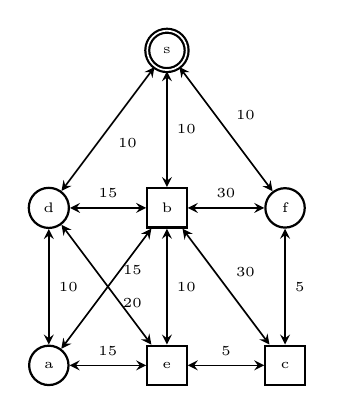
\begin{tikzpicture}[
            > = stealth, % arrow head style
            %shorten > = 0.7pt, % don't touch arrow head to node
            auto,
            node distance = 0.3cm, % distance between nodes
            semithick, % line style
            font=\tiny,
            align=center
        ]

        \tikzstyle{every state}=[
            draw = black,
            thick,
%            fill = black,
            minimum size = 5mm
        ]

        \node[state, double] (s) [at={(0, 0)}] {s};
        \node[state] (d) [at={(-1.5, -2)}] {d};
        \node[state, rectangle] (b) [at={(0, -2)}] {b};
        \node[state] (f) [at={(1.5, -2)}] {f};
        \node[state] (a) [at={(-1.5, -4.0)}] {a};
        \node[state, rectangle] (e) [at={(0, -4.0)}] {e};
        \node[state, rectangle] (c) [at={(1.5, -4.0)}] {c};
                        
        \path[<->] (s) edge node {10} (d);
        \path[<->] (s) edge node {10} (b);
        \path[<->] (s) edge node {10} (f);
        \path[<->] (d) edge node {10} (a);
        \path[<->] (d) edge node {\ 15} (e);
        \path[<->] (b) edge node {30} (c);
        % Fake edges
        \path[<->] (d) edge node {15} (b);
        \path[<->] (f) edge node {5} (c);
        \path[<->] (b) edge node {30} (f);
        \path[<->] (b) edge node {10} (e);
        \path[<->] (b) edge node {\ 20} (a);
        \path[<->] (e) edge node {5} (c);
        \path[<->] (a) edge node {15} (e);        
    \end{tikzpicture}
\subcaption{\label{subfig:graph} Grafo $G$}
\end{subfigure} \hfill
\begin{subfigure}{.5\textwidth}
\centering
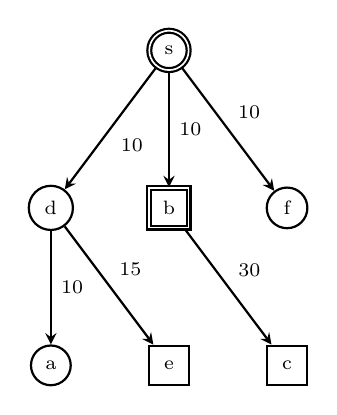
\begin{tikzpicture}[
            > = stealth, % arrow head style
            %shorten > = 0.7pt, % don't touch arrow head to node
            auto,
            node distance = 0.2cm, % distance between nodes
            thick, % line style
            font=\scriptsize,
            align=center
  ]

        \tikzstyle{every state}=[
            draw = black,
            thick,
%            fill = black,
            minimum size = 5mm
        ]

        \node[state, double] (s) [at={(0, 0)}] {s};
        \node[state] (d) [at={(-1.5, -2)}] {d};
        \node[state, double, rectangle] (b) [at={(0, -2)}] {b};
        \node[state] (f) [at={(1.5, -2)}] {f};
        \node[state] (a) [at={(-1.5, -4.0)}] {a};
        \node[state, rectangle] (e) [at={(0, -4.0)}] {e};
        \node[state, rectangle] (c) [at={(1.5, -4.0)}] {c};
                
        
        \path[->] (s) edge node {10} (d);
        \path[->] (s) edge node {10} (b);
        \path[->] (s) edge node {10} (f);
        \path[->] (d) edge node {10} (a);
        \path[->] (d) edge node {15} (e);
        \path[->] (b) edge node {30} (c);
        % Fake edges
        %\path[<->, opacity = 0.3] (d) edge node {} (b);
        %\path[<->, opacity = 0.3] (c) edge node {} (f);
        %\path[<->, opacity = 0.3] (b) edge node {} (f);
        %\path[<->, opacity = 0.3] (e) edge node {} (b);
        %\path[<->, opacity = 0.3] (b) edge node {} (a);
        %\path[<->, opacity = 0.3] (e) edge node {} (c);
        %\path[<->, opacity = 0.3] (a) edge node {} (e);        
    \end{tikzpicture}
\subcaption{\label{subfig:arb-t} Arborescência $T$}
\end{subfigure}
\\
\begin{subfigure}{.3\textwidth}
\centering
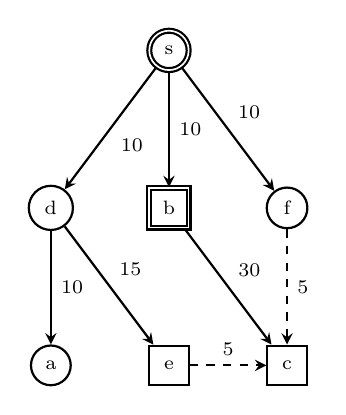
\begin{tikzpicture}[
            > = stealth, % arrow head style
            %shorten > = 0.7pt, % don't touch arrow head to node
            auto,
            node distance = 0.2cm, % distance between nodes
            thick, % line style
            font=\scriptsize
  ]

        \tikzstyle{every state}=[
            draw = black,
            thick,
%            fill = black,
            minimum size = 5mm
        ]

        \node[state, double] (s) [at={(0, 0)}] {s};
        \node[state] (d) [at={(-1.5, -2)}] {d};
        \node[state, double, rectangle] (b) [at={(0, -2)}] {b};
        \node[state] (f) [at={(1.5, -2)}] {f};
        \node[state] (a) [at={(-1.5, -4.0)}] {a};
        \node[state, rectangle] (e) [at={(0, -4.0)}] {e};
        \node[state, rectangle] (c) [at={(1.5, -4.0)}] {c};
                
        
        \path[->] (s) edge node {10} (d);
        \path[->] (s) edge node {10} (b);
        \path[->] (s) edge node {10} (f);
        \path[->] (d) edge node {10} (a);
        \path[->] (d) edge node {15} (e);
        \path[->] (b) edge node {30} (c);
        % Fake edges
        %\path[<->, opacity = 0.3] (d) edge node {} (b);
        \path[->, style = dashed] (f) edge node {5} (c);
        %\path[<->, opacity = 0.3] (b) edge node {} (f);
        %\path[<->, opacity = 0.3] (e) edge node {} (b);
        %\path[<->, opacity = 0.3] (b) edge node {} (a);
        \path[->, style = dashed] (e) edge node {5} (c);
        %\path[<->, opacity = 0.3] (a) edge node {} (e);        
    \end{tikzpicture}
\subcaption{\label{subfig:ver-c} Verifica nó $c$}
\end{subfigure} \hfill
% e
\begin{subfigure}{.3\textwidth}
\centering
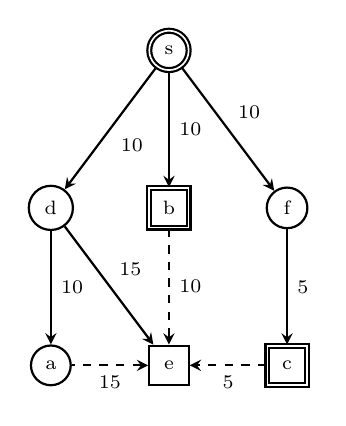
\begin{tikzpicture}[
            > = stealth, % arrow head style
            %shorten > = 0.7pt, % don't touch arrow head to node
            auto,
            node distance = 0.2cm, % distance between nodes
            thick, % line style
            font=\scriptsize
  ]

        \tikzstyle{every state}=[
            draw = black,
            thick,
%            fill = black,
            minimum size = 5mm
        ]

        \node[state, double] (s) [at={(0, 0)}] {s};
        \node[state] (d) [at={(-1.5, -2)}] {d};
        \node[state, double, rectangle] (b) [at={(0, -2)}] {b};
        \node[state] (f) [at={(1.5, -2)}] {f};
        \node[state] (a) [at={(-1.5, -4.0)}] {a};
        \node[state, rectangle] (e) [at={(0, -4.0)}] {e};
        \node[state, double, rectangle] (c) [at={(1.5, -4.0)}] {c};
                
        
        \path[->] (s) edge node {10} (d);
        \path[->] (s) edge node {10} (b);
        \path[->] (s) edge node {10} (f);
        \path[->] (d) edge node {10} (a);
        \path[->] (d) edge node {15} (e);
        \path[->] (f) edge node {5} (c);
        % Fake edges
        \path[->, style = dashed] (b) edge node {10} (e);
        \path[->, style = dashed] (c) edge node {5} (e);
        \path[<-, style = dashed] (e) edge node {15} (a);
        %\path[<->, opacity = 0.3] (e) edge node {} (b);
        %\path[<->, opacity = 0.3] (b) edge node {} (a);
        %\path[->, style = dashed] (e) edge node {5} (c);
        %\path[<->, opacity = 0.3] (a) edge node {} (e);        
    \end{tikzpicture}
\subcaption{\label{subfig:ver-e} Verifica nó $e$}
\end{subfigure} \hfill
% final
\begin{subfigure}{.3\textwidth}
\centering
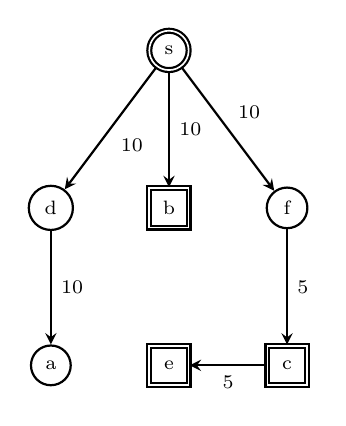
\begin{tikzpicture}[
            > = stealth, % arrow head style
            %shorten > = 0.7pt, % don't touch arrow head to node
            auto,
            node distance = 0.2cm, % distance between nodes
            thick, % line style
            font=\scriptsize
  ]

        \tikzstyle{every state}=[
            draw = black,
            thick,
%            fill = black,
            minimum size = 5mm
        ]

        \node[state, double] (s) [at={(0, 0)}] {s};
        \node[state] (d) [at={(-1.5, -2)}] {d};
        \node[state, double, rectangle] (b) [at={(0, -2)}] {b};
        \node[state] (f) [at={(1.5, -2)}] {f};
        \node[state] (a) [at={(-1.5, -4.0)}] {a};
        \node[state, double, rectangle] (e) [at={(0, -4.0)}] {e};
        \node[state, double, rectangle] (c) [at={(1.5, -4.0)}] {c};
                
        
        \path[->] (s) edge node {10} (d);
        \path[->] (s) edge node {10} (b);
        \path[->] (s) edge node {10} (f);
        \path[->] (d) edge node {10} (a);
        \path[->] (c) edge node {5} (e);
        \path[->] (f) edge node {5} (c);
        % Fake edges
        %\path[->, style = dashed] (b) edge node {10} (e);
        %\path[->] (c) edge node {5} (e);
        %\path[<-, style = dashed] (e) edge node {15} (a);
        %\path[<->, opacity = 0.3] (e) edge node {} (b);
        %\path[<->, opacity = 0.3] (b) edge node {} (a);
        %\path[->, style = dashed] (e) edge node {5} (c);
        %\path[<->, opacity = 0.3] (a) edge node {} (e);        
    \end{tikzpicture}
\subcaption{\label{subfig:arb-final} Arborescência final}
\end{subfigure}
\caption{Exemplo de aplicação da busca local \label{fig:exemplo-busca}}
\end{figure}

Com  a  alteração do  predecessor  de  $c$  validada,  repete-se o  processo  de
verificação  e   busca  para  o   terminal  $e$,  como  apresentado   na  Figura
\ref{subfig:ver-e}. Para este caso, existem três possibilidades, mas apenas duas
são viáveis. Alterar  o predecessor de $e$ para  $b$ ou $c$ faz com  que o valor
$L[e]$ seja reduzido de 25 para  20, tornando-o atendido em {\delay} e variação.
Por fim,  assumindo a seleção  do arco $(c, e)$,  temos como resultado  a Figura
\ref{subfig:arb-final} que  apresenta a  arborescência final do  procedimento de
busca local, atendendo os três terminais.

\begin{comment}
 efetuar  modificações em  arcos
adjacentes  à  nós  terminais  visando aproximar,  seja  reduzindo  ou
incrementando,  os custos  em delay  dos  caminhos e  assim reduzir  a
quantidade de nós  que deixam de ser atendidos por  conta da restrição
de variância \eqref{eq:mod-var-delay}.   Um Pseudocódigo é apresentado
em \ref{alg:heuristic-subgrad}.

As  linhas  \eqref{line:graph}-\eqref{line:vetores}  são  apenas  para
declaração e inicialização das estruturas utilizadas pelo algoritmo. O
laço                             das                            linhas
\eqref{line:primeiro-laco}-\eqref{line:final-primeiro-laco} inicializa
os vetores, armazenando os caminhos que  vão da raiz (s) para todos os
demais nós  da arborescência ($T$) e  os custos em delay  e jitter dos
caminhos,  caso o  nó em  questão seja  terminal e  os custos  excedam
$\Delta_d$ ou $\Delta_j$  deve-se marcar este nó como  não atendido. O
próximo passo é  selecionar, de maneira aleatória, um  nó terminal $f$
como representado  na linha  \eqref{line:selec-fixed}, $f$  deve estar
marcado como  atendido e  seu caminho  ou custo  não será  alterado em
nenhum passo posterior da heurística, o  intuito é utilizar o custo de
delay do caminho  para $f$ como ponto fixo, focando  em incrementar ou
reduzir, sem  deixar de atender,  o custo  em delay dos  caminhos para
demais  terminais de  modo que  estejam dentro  da ``janela''  que não
viola a restrição de variância, ou seja, $custoDelay[f] \pm \Delta_v$.

O      procedimento      contido      no     laço      das      linhas
\eqref{line:loop-busca-inicio}-\eqref{line:loop-busca-fim}    percorre
todo $k \in  D$ com exceção de $f$  e verifica se o valor  de delay do
caminho    para   $k$    está    fora   do    intervalo   da    janela
\eqref{line:is-irregular}, nesse  caso todos  os arcos que  incidem em
$k$  serão   avaliados  \eqref{line:busca-vizinhanca}  e   caso  algum
respeite as  restrições da linha  \eqref{line:movimento-permitido}, ou
seja, a alteração no arco  mantém as propriedades da arborescência, os
novos custos de delay e jitter não excedam $\Delta_d$ e $\Delta_j$ e o
delay está  dentro da  janela definida, então  esse movimento  é salvo
como viável. Ao  final da avaliação dos arcos, caso  exista mais de um
movimento, seleciona-se  aquele que  tem o  menor custo  em delay  e a
alteração  do  arco  e  dos  custos  é  feita  de  maneira  temporária
\eqref{line:mov-mais-barato}.   A   intuição  por  trás   deste  passo
consiste em economizar o recurso de  delay ao máximo no atendimento do
nó $k$  deixando assim  uma margem  que permita  um maior  conjunto de
movimentos para os possíveis terminais  que são alcançados a partir de
$k$.     Com     isso,     utiliza-se    o     laço     das     linhas
\eqref{line:laco-prop}-\eqref{line:laco-prop-fim}   para   avaliar   o
efeito da troca do  arco no caminho para $k$, pois  os custos de todos
os nós que são  alcançáveis a partir de $k$ em $T$  tem seus custos de
jitter e delay atualizados e caso  a alteração dos custos faça com que
2 ou mais outros terminais deixem de  ser atendidos, a troca do arco é
desconsiderada  e todas  as  alterações feitas  são descartadas,  caso
contrário a alteração em $T$ e realizada.

Ao   final    da   busca    nos   caminhos   utiliza-se    as   linhas
\eqref{line:cont-menor}-   \eqref{line:cont-maior}   para   contar   a
quantidade  de  caminhos  que  tem custo  de  delay,  respectivamente,
menores e maiores que $custoDelay[f]$,  essa contagem serve de auxílio
para             o             laço             das             linhas
\eqref{line:laco-marcar-vari-inicio}-\eqref{line:laco-marcar-vari-fim}
que  tem como  objetivo  decidir,  sempre que  algum  par  de nós  não
respeitar  a  restrição  de  variância, qual  deles  marcar  como  não
atendido. Como  o intuito  do algoritmo  é fazer com  que o  delay dos
caminhos  esteja em  um intervalo  de  janela em  relação ao  terminal
fixado,  se  houverem mais  caminhos  com  custo  de delay  abaixo  de
$custoDelay[f]$ então no caso de um par de terminais violar $\Delta_v$
iremos marcar como  não atendido aquele cujo custo de  delay for maior
que $custoDelay[f]$. A mesma ideia se  mantém para o caso onde a maior
quantidade   de  caminhos   estão  com   custo  de   delay  acima   de
$custoDelay[f]$.
\end{comment}

\section{Análise Estatística de Resultados} \label{sec:analise-statistica}

Neste trabalho, utilizaram-se testes  estatísticos não paramétricos para análise
de múltiplas  instâncias. O objetivo da  utilização desses testes é  fornecer um
embasamento  científico  mais  rígido  às comparações  feitas,  validando  se  a
diferença entre  duas ou  mais estratégias  é estatisticamente  significativa ou
não. O  trabalho de  Dem\v{s}ar \cite{demsar:2006}  sugere uma  metodologia para
fazer  tais  comparações  no  contexto   de  aprendizado  de  máquina,  no  qual
utilizam-se  diversos testes,  de  modo a  identificar  existência de  diferença
estatisticamente significativa  (DES) entre vários classificadores  em múltiplos
conjuntos de dados. Nesta seção, serão brevemente discutidos os testes e a forma
de interpretação de seus resultados.

Para todos  os testes  foi considerado  um nível  de confiança  de $95\%$  com a
hipótese  nula de  que não  existe DES  entre as  amostras. Todos  os testes  se
baseiam em \textit{ranks},  de modo que a abordagem que  detém \textit{rank k} é
aquela contendo o k-ésimo melhor resultado para uma instância.

O  primeiro teste  descrito é  o de  Iman-Davenport, utilizado  para identificar
existência de DES entre múltiplas abordagens. Inicialmente precisa-se computar o
valor de  \textit{rank} médio $R_i$  para cada abordagem.  O cálculo é  feito da
seguinte forma: seja $r_k^i$ o \textit{rank} da k-ésima abordagem para a i-ésima
instância (com \textit{rank} médio sendo utilizado  em caso de empates). O valor
$R_i$ para  a i-ésima metodologia é  dado por $R_i =  \frac{1}{N} \cdot \sum_{k}
r_k^i, \forall k  \in \{1, \dots, k\}$, tal  que $k$ é o número  de abordagens e
$N$ o número de instâncias.

O  valor do  teste  de Iman-Davenport  é  calculado de  acordo  com as  equações
\eqref{eq:x2f} e \eqref{eq:ff}.

\begin{equation}
    x^2_F = \frac{12 \cdot N}{k \cdot (k + 1)} \left[ \sum_{i} R^2_{i} - \frac{k \cdot (k+1)^2}{4} \right] \label{eq:x2f}
\end{equation}

\begin{equation}
    F_F = \frac{(N - 1) \cdot x^2_F}{N \cdot (k - 1) - x^2_F} \label{eq:ff}
\end{equation}

O valor do teste calculado para $F_F$  segue a distribuição $F$, a qual tem como
parâmetros os graus  de liberdade, $k -  1$ e $(k -  1) \cdot (N -  1)$. Logo, o
valor crítico  pode ser obtido seguindo  tal distribuição. Ao final,  se o valor
$F_F$ encontrado  pelo teste for maior  que o valor crítico,  pode-se rejeitar a
hipótese nula.

Caso  a  hipótese  nula  seja  rejeitada, inicia-se  a  aplicação  de  um  teste
\textit{post-hoc} para encontrar quais das heurísticas de fato diferem entre si.
Para  tal, utiliza-se  o teste  de Nemenyi,  que calcula  a diferença  crítica e
identifica grupos de abordagens que  são estatisticamente equivalentes entre si.
Os resultados de duas abordagens distintas são ditos diferentes, segundo o teste
de Nemenyi, se seus \textit{ranks} médios  se diferem por pelo menos a diferença
crítica (DC) obtida segundo a equação \eqref{eq:dc}.

\begin{equation}
    DC = q_{\alpha} \cdot \sqrt{\frac{l \cdot (k + 1)}{6 \cdot N}} \label{eq:dc}
\end{equation}

Na equação \eqref{eq:dc}, o $\alpha$ representa  o nível de confiança, e o valor
crítico  $q_{\alpha}$ é  definido segundo  a estatística  de \textit{Studentized
range}  dividida  por  $\sqrt{2}$.  Os  valores de  tal  estatística  podem  ser
encontrados no  artigo de De\v{m}sar  \cite{demsar:2006}. Ainda, o  resultado do
teste de  Nemenyi pode ser  representado graficamente, como ilustrado  na Figura
\ref{fig:ex-nemenyi}. O  eixo horizontal  equivale aos valores  de \textit{rank}
médio,  em  ordem  crescente  da  esquerda para  a  direita.  Cada  abordagem  é
representada  por  uma  linha  vertical  com seu  respectivo  nome  e  valor  de
\textit{rank} médio logo abaixo. Uma linha horizontal de comprimento equivalente
ao valor da DC é posicionada  acima do eixo horizontal principal. Abordagens nas
quais o valor de \textit{rank} médio não diferem mais do que a DC são conectadas
por um segmento  horizontal em negrito, de comprimento sempre  inferior ao valor
da DC.

\begin{figure}[!ht] \centering
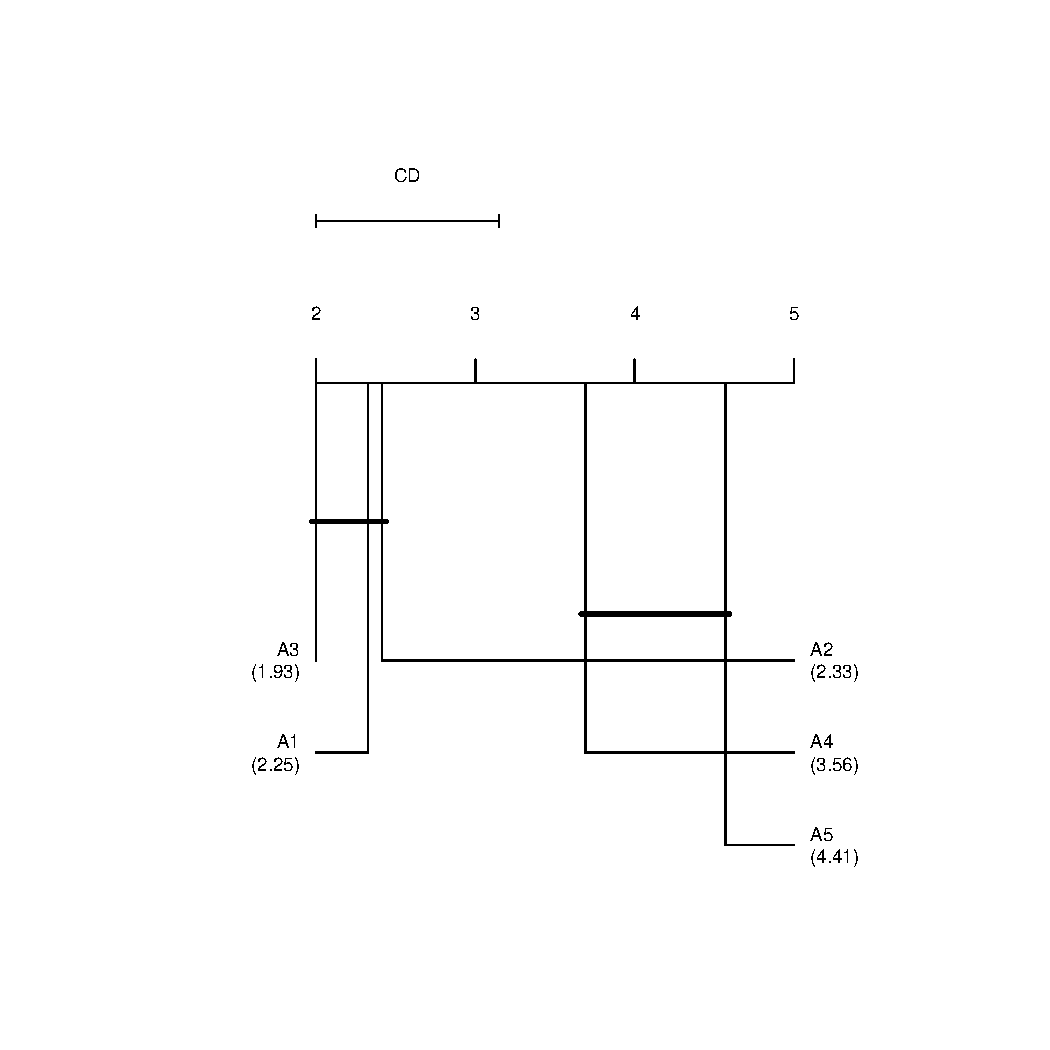
\includegraphics[scale=0.4]{imagens/exemplo-nemenyi.pdf}
    \caption{Exemplo de representação gráfica do teste Nemenyi.}
    \label{fig:ex-nemenyi}
\end{figure}

Observa-se que as abordagens fictícias A3, A1 e A2 formam o grupo de menor valor
de \textit{rank}  médio, e  consequentemente, são  estatisticamente equivalentes
entre si de acordo com o teste de Nemenyi. Portanto, podemos definir como melhor
algoritmo aquele  que apresenta o  maior número de  vitórias, i.e., o  número de
vezes que cada abordagem foi melhor que as demais.

Outro  teste  utilizado  neste  trabalho  foi o  de  Wilcoxon,  aplicado  quando
deseja-se verificar  se existe DES  entre os  resultados de dois  métodos, sendo
mais  poderoso que  o teste  de  Iman-Davenport para  esse cenário.  O teste  de
Wilcoxon computa os  \textit{ranks} das diferenças entre os  resultados dos dois
métodos  ignorando  o  sinal  e posteriormente  compara  os  \textit{ranks}  das
diferenças positivas e negativas.

Para computar  o teste de  Wilcoxon, considere $d_i, i  \in \{1, \dots,  N\}$, a
diferença  entre  os  resultados  das  duas  abordagens  na  i-ésima  instância,
$r_{d_i}$ o \textit{rank} do valor  absoluto da i-ésima diferença (\textit{rank}
médio é  atribuído no caso  de empate). Assuma  $R^+$ a soma  dos \textit{ranks}
para as instâncias nas quais a abordagem fictícia  A foi melhor do que B ($d_i >
0$) e  $R^{-}$ a  soma dos  \textit{ranks} para o  caso oposto  ($d_i <  0$). Os
\textit{ranks} para  $d_i =  0$ são  separados igualmente  entre as  somas, como
mostrado na Equação \eqref{eq:r-wilcoxon}.

\begin{equation}
    R^{+} = \sum_{d_i > 0} r_{d_i} + \frac{1}{2}\sum_{d_i = 0} \quad \quad R^{-} = \sum_{d_i < 0} r_{d_i} + \frac{1}{2}\sum_{d_i = 0} \label{eq:r-wilcoxon}
\end{equation}

Seja T = $\min\{R^+, R^{-}\}$ . Segundo Dem\v{s}ar \cite{demsar:2006}, nos casos
onde $N \leq 25$,  o valor crítico para o teste de  Wilcoxon pode ser consultado
na  maioria  dos   livros  de  estatística,  como  por  exemplo,   o  de  Devore
\cite{devore:2011}. Uma  vez que  tal valor é  calculado, rejeita-se  a hipótese
nula se o valor de $T$ for menor ou  igual ao valor crítico. No caso em que $N >
25$, computa-se a estatística $z$ como apresentado na Equação \eqref{eq:z-stat}.
Segundo Dem\v{s}ar,  considerando um  nível de confiança  de $95\%$,  a hipótese
nula pode ser rejeitada quando $z < -1.96$.

\begin{equation}
    z = \frac{T - \frac{1}{4} N(N + 1)}{\sqrt{\frac{1}{24} N(N+1)(2N + 1)}} \label{eq:z-stat}
\end{equation}

\section{Geração de Instâncias} \label{sec:instance-generation}

Nos  trabalhos presentes  na literatura  que envolvem  o problema  de roteamento
aplicado a redes veiculares,  não há um consenso entre os  autores em relação às
instâncias utilizadas em  experimentos. Cada autor criou  as próprias instâncias
para validação  do algoritmo  ou protocolo proposto,  como pode-se  observar nos
trabalhos  de   \cite{BITAM2013981,  fazio:2013,   tiago:2019}.  A   geração  de
instâncias descrita nesta  seção é fortemente baseada no trabalho  de Ribeiro et
al. \cite{tiago:2019},  que descreve  uma maneira  coerente de  criar instâncias
para  avaliação  de  algoritmos  de roteamento  em  VANET's  utilizando  modelos
baseados  em simulação  de tráfego.  Nessa  simulação é  possível visualizar  os
movimentos dos  veículos que  são gerados,  além de poder  exportar os  dados de
mobilidade, ou  seja, o posicionamento,  velocidade e  direção de um  veículo em
determinado  instante. Os  dados exportados  do modelo  de mobilidade  podem ser
introduzidos em  um simulador  específico para redes  de comunicação,  como NS-2
\cite{Issariyakul:2010}, NS-3 \cite{Riley2010} e OMNet \cite{Varga:2008}.

Para a  simulação de tráfego e  mobilidade veicular tratada neste  trabalho, foi
escolhida a biblioteca  SUMO (\textit{Simulation of Urban MObility}),  que é uma
ferramenta amplamente  utilizada tanto no  meio acadêmico quanto  empresarial. O
SUMO é acoplado a uma ferramenta externa de simulação de redes, neste caso NS-2,
para fornecer dados realistas de comunicação dos veículos. O NS-2 é um simulador
de eventos discretos direcionados à  pesquisa de rede, inicialmente desenvolvido
pela Universidade de Berkeley e  altamente utilizado pela comunidade científica.
O  NS-2 fornece  um  apoio  substancial para  a  simulação  do funcionamento  de
transmissões, roteamento  e protocolos  de redes,  com e  sem fio.  É importante
utilizar o modelo de mobilidade gerado  pelos simuladores de veículos para que o
posicionamento dos nós esteja o mais próximo possível da realidade.

O  primeiro passo  na geração  de instâncias  para o  \gls{pma} é  a criação  de
estradas  e  rodovias.  Neste  trabalho   foram  adotados  como  base  os  mapas
disponíveis no projeto \textit{Open  Street Maps} (OSM) \cite{harklay:2008}, que
é um projeto de  mapeamento colaborativo para criar um mapa  livre e editável do
mundo e está  em desenvolvimento desde 2004.  A Figura \ref{fig:map-open-street}
apresenta  uma   parte  do  mapa  da   cidade  de  Washington  D.   C.,  medindo
aproximadamente 250.000 metros quadrados.

\begin{figure}[!ht]
    \centering
    \fbox{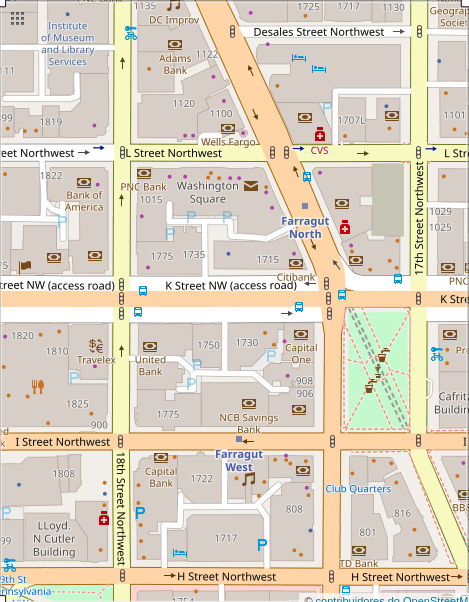
\includegraphics[scale = 0.35]{imagens/map-open-street.png}}
    \caption{Parte do mapa da cidade de Washington no \textit{Open Street Maps}}
    \label{fig:map-open-street}
\end{figure}

O passo seguinte  é tratar e selecionar  as informações desejadas com  o OSM, ou
seja, o  recorte do  mapa que  se deseja  utilizar. Os  dados são  convertidos e
importados para o SUMO gerando assim  o modelo de mobilidade, inserindo veículos
no mapa,  bem como  semáforos e  outros componentes  inerentes ao  tráfego. Após
essas  inserções,  inicia-se  o  processo  de  simulação  do  tráfego  veicular,
exportando  os dados  de  movimentação  dos veículos  para  utilização na  etapa
posterior. A Figura  \ref{fig:map-sumo} apresenta uma parte ampliada  do mapa de
Washington, ressaltando dados de tráfego e veículos.

\begin{figure}[!ht]
    \centering
    \fbox{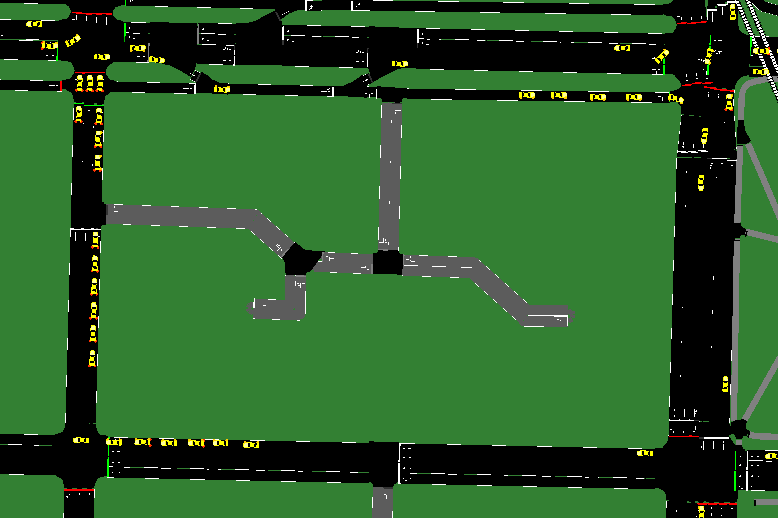
\includegraphics[scale = 0.35]{imagens/map-sumo.png}}
    \caption{Parte do mapa ampliado da cidade de Washington no SUMO}
    \label{fig:map-sumo}
\end{figure}

Após a exportação dos dados vindos do SUMO, será feita a utilização do simulador
de rede  NS-2. O processo  de simulação  de rede é  então iniciado e,  durante o
mesmo, é possível fotografar um momento qualquer e com isso obter a topologia da
rede como um todo,  representando-a como um grafo. O valor  das métricas em cada
\textit{link} é medido com base na troca de mensagem entre os pares de veículos.
Considera-se o  cálculo médio em um  intervalo de 15 segundos.  Assim é possível
ter uma  instância próxima da  realidade, dentro  das limitações do  processo de
simulação.

A Figura \ref{fig:instance}  ilustra o grafo da instância final  gerada a partir
de  um intervalo  de tempo  da  simulação. Os  nós não  seguem o  posicionamento
geográfico real, apenas exibem as conexões existentes naquele intervalo entre os
10 veículos da rede. O nó azul representa a origem, os nós vermelhos representam
os destinos, ambos  decididos aleatoriamente. Os nós pretos são  nós de Steiner,
que  podem  ser   utilizados  ou  não  no  processo  de   construção  da  árvore
\textit{multicast}.

\begin{figure}[!ht]
    \centering
    \fbox{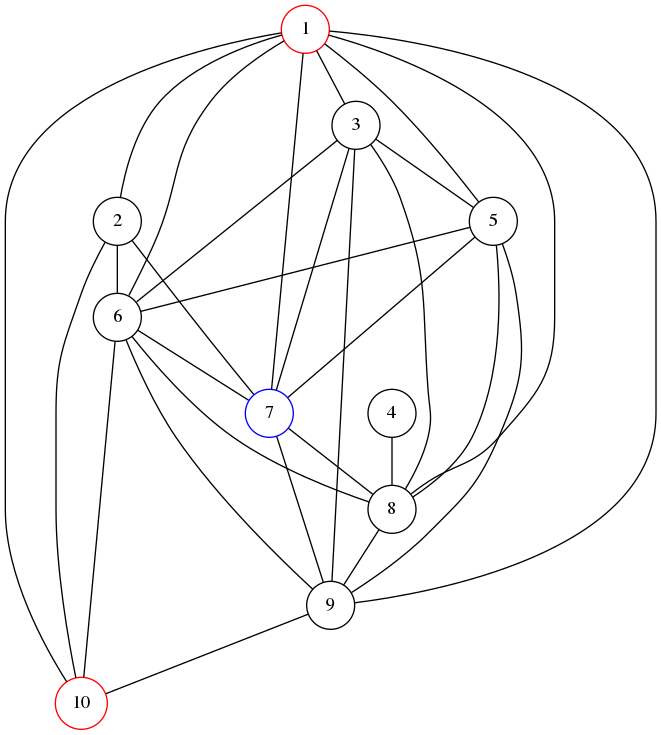
\includegraphics[scale = 0.3]{imagens/instance.png}}
    \caption{Fotografia dos enlaces da rede.}
    \label{fig:instance}
\end{figure}

Outros parâmetros  da instância são os  valores máximos de {\delay}  e {\jitter}
permitidos no  caminho da  raiz até  cada um  dos terminais,  o valor  máximo da
variação de  {\delay} entre o  nó origem  e qualquer par  de destinos e  o valor
mínimo  de largura  de  banda dos  arcos. Foram  gerados  diferentes valores  de
parâmetros  visando  estressar  as  metodologias   na  etapa  de  avaliação  dos
algoritmos.  Para tal,  foram geradas  duas árvores  de caminhos  mínimos do  nó
origem para todos os nós destino. A primeira é calculada utilizando como custo o
{\delay} dos arcos e a segunda o {\jitter}. Essas árvores são referenciadas como
$T^d$ e $T^j$, respectivamente.

Seja $\lambda^{*}$ o maior valor de  {\delay} entre os caminhos da árvore $T^d$.
A partir da árvore  $T^j$, é possível inverter os custos  de {\jitter} dos arcos
pelos  de {\delay}  e assim  obter  $\tilde{\lambda}$, que  é o  maior valor  de
{\delay} nos caminhos  da árvore de {\jitter}, ou seja,  $T^j$. Seguindo o mesmo
procedimentos,   obtém-se   os   valores  $\xi^{*}$   e   $\tilde{\xi}$,   sendo
respectivamente o maior valor de {\jitter} da árvore $T^j$ e da árvore $T^d$.

Para  a  geração   das  instâncias,  os  parâmetros   foram  configurados  como:
$\Delta_{d} = \tilde{\lambda}$  e $\Delta_{j} = \tilde{\xi}$. O  valor do mínimo
de largura  de banda  necessária para o  link foi fixado  em 200,  utilizando um
parâmetro  aplicado  diretamente  ao  simulador  de  rede.  Por  fim,  assumindo
$\lambda^1,  \dots, \lambda^{|D|}$  como  os valores  de  {\delay} dos  caminhos
mínimos para cada terminal na árvore $T^d$, obtém-se o valor de $\Delta_v$ igual
ao desvio  padrão da diferença  absoluta entre todos os  pares de {\delay  s} em
$\lambda^1, \dots, \lambda^{|D|}$.

A  Figura  \ref{fig:flowchart},  retirada  de  \cite{tiago:2019},  apresenta  um
fluxograma simplificado  do processo de  geração das instâncias,  começando pelo
processo de extração do mapa, passando  pela simulação de tráfego usando o SUMO,
juntamente com  a criação do  modelo de mobilidade  e terminando no  processo de
simulação  no NS-2,  onde  a instância  final  é gerada.  O  conjunto de  testes
desenvolvido neste trabalho  é formado por 40 instâncias criadas  a partir de um
trecho real do mapa da cidade de Washington. Para 30 instâncias o número de nós
varia de 10 a 100,  o número de terminais de 4 a 52 e o  número de arcos de 18 a
4416. Para 10 outras instâncias, o número de nós varia de 125 a 350, o número de
terminais de 55 a 170 e o número de arcos de 2448 a 24446.

\begin{figure}[!ht]
    \centering
    \fbox{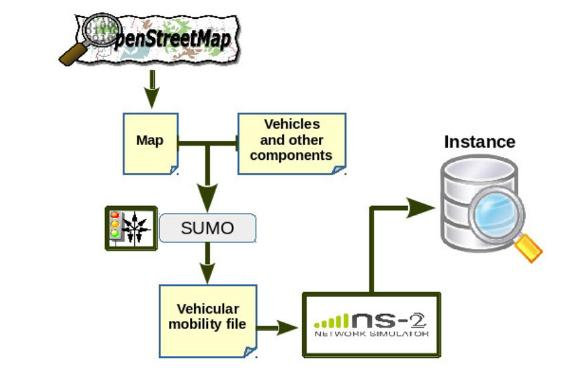
\includegraphics[scale = 0.5]{imagens/flowchart.jpg}}
    \caption{Fluxograma do processo de geração das instâncias.}
    \label{fig:flowchart}
\end{figure}

\begin{comment}
Os  grafos das  instâncias foram  gerados  com base  em 4  recortes de  tamanhos
diferentes do mapa  da cidade de Washington DC, $50^{2}$,  $75^{2}$, $100^{2}$ e
$200^{2}$ na escala de distância da  própria ferramenta. Para cada recorte foram
criadas  10  instâncias,  para  os  3 recortes  menores  o  número  de  veículos
considerados para  o grafo variou  de 10  à 100. Para  o recorte de  $200^{2}$ o
número de veículos foi de 125 a 350. O número de conexões variou de acordo com a
simulação  de  rede  e o  percurso  dos  veículos,  mas  o objetivo  foi  formar
instâncias mais densas  no recorte menor e ir torná-las  mais esparsas de acordo
com o  aumento de  tamanho do trecho  do mapa. O  nós raiz  e o conjunto  de nós
terminais  são selecionado  aleatoriamente, sendo  o número  de terminais  em um
intervalo de $40\%$ a $60\%$ do número de nós. O nome de cada instância é gerado
no  seguinte  padrão  ``washington-tamanho do  recorte-$|V|$-$|D|$''.  A  Tabela
\ref{tab:met-instancias} contém  os dados  de cada  instância, juntamente  com o
número de  conexões, denominado por $E$,  ou seja, não é  considerada direção na
conexão.

\begin{table}[!ht]
\centering
\footnotesize{%
\begin{tabular}{llrlrlr}
\hline
\multicolumn{1}{c}{\textbf{Instância}} & \multicolumn{1}{c}{\textbf{}} & \multicolumn{1}{c}{\textbf{|V|}} & \multicolumn{1}{c}{\textbf{}} & \multicolumn{1}{c}{\textbf{|D|}} & \multicolumn{1}{c}{\textbf{}} & \multicolumn{1}{c}{\textbf{|E|}} \\ \hline
washington-50-10-6 &  & 10 &  & 6 &  & 23 \\
washington-50-20-11 &  & 20 &  & 11 &  & 92 \\
washington-50-30-15 &  & 30 &  & 15 &  & 210 \\
washington-50-40-23 &  & 40 &  & 23 &  & 415 \\
washington-50-50-28 &  & 50 &  & 28 &  & 624 \\
washington-50-60-35 &  & 60 &  & 35 &  & 906 \\
washington-50-70-37 &  & 70 &  & 37 &  & 1258 \\
washington-50-80-39 &  & 80 &  & 39 &  & 1796 \\
washington-50-90-51 &  & 90 &  & 51 &  & 2109 \\
washington-50-100-45 &  & 100 &  & 45 &  & 2208 \\ \hline
washington-75-10-4 &  & 10 &  & 4 &  & 16 \\
washington-75-20-12 &  & 20 &  & 12 &  & 63 \\
washington-75-30-16 &  & 30 &  & 16 &  & 159 \\
washington-75-40-21 &  & 40 &  & 21 &  & 269 \\
washington-75-50-30 &  & 50 &  & 30 &  & 438 \\
washington-75-60-25 &  & 60 &  & 25 &  & 628 \\
washington-75-70-42 &  & 70 &  & 42 &  & 850 \\
washington-75-80-48 &  & 80 &  & 48 &  & 1252 \\
washington-75-90-47 &  & 90 &  & 47 &  & 1517 \\
washington-75-100-52 &  & 100 &  & 52 &  & 1896 \\ \hline
washington-100-10-6 &  & 10 &  & 6 &  & 9 \\
washington-100-20-10 &  & 20 &  & 10 &  & 49 \\
washington-100-30-12 &  & 30 &  & 12 &  & 103 \\
washington-100-40-18 &  & 40 &  & 21 &  & 211 \\
washington-100-50-27 &  & 50 &  & 27 &  & 298 \\
washington-100-60-34 &  & 60 &  & 34 &  & 427 \\
washington-100-70-39 &  & 70 &  & 39 &  & 602 \\
washington-100-80-32 &  & 80 &  & 32 &  & 882 \\
washington-100-90-43 &  & 90 &  & 43 &  & 1151 \\
washington-100-100-43 &  & 100 &  & 43 &  & 1408 \\ \hline
washington-200-125-55 &  & 125 &  & 55 &  & 1224 \\
washington-200-150-61 &  & 150 &  & 61 &  & 2234 \\
washington-200-175-74 &  & 175 &  & 74 &  & 3024 \\
washington-200-200-114 &  & 200 &  & 114 &  & 3645 \\
washington-200-225-135 &  & 225 &  & 135 &  & 4464 \\
washington-200-250-109 &  & 250 &  & 109 &  & 6403 \\
washington-200-275-146 &  & 275 &  & 146 &  & 7195 \\
washington-200-300-136 &  & 300 &  & 136 &  & 8709 \\
washington-200-325-170 &  & 325 &  & 170 &  & 9260 \\
washington-200-350-150 &  & 350 &  & 150 &  & 12218 \\ \hline
\end{tabular}%
}
\caption{Sumário das instâncias}
\label{tab:met-instancias}
\end{table}
\end{comment}
\chapter{Resultados Computacionais} \label{chp:resultados}

Neste capítulo são descritos os  experimentos realizados para avaliar a eficácia
das  diversas  abordagens  propostas   nesta  dissertação.  Este  capítulo  está
organizado  da seguinte  maneira: a  Seção~\ref{sec:prep} contém  as informações
sobre os  pré-processamentos, seguida da Seção~\ref{sec:modelos},  que apresenta
os resultados dos modelos de \gls{pli} e \gls{plim} desenvolvidos.

%   dos   modelos   matemáticos   propostos  nas   Seções   \ref{sec:dmfm-pma}   e
% \ref{sec:ab-pma} juntamente  com o  impacto dos pré-processamentos  descritos na
% Seção  \ref{subsec:prep};   as  relaxações   lagrangianas  descritas   na  Seção
% \ref{sec:rl-pma}   e  as   variações  do   \gls{brkga}  apresentadas   na  Seção
% \ref{sec:brkga}.

As estratégias apresentadas foram implementadas  em C++, os programas compilados
com GCC  versão 7.5.0, usando o  nível de otimização -O3.  Os experimentos foram
realizados em um  processador Intel(R) Xeon(R) CPU E5-2630 v4  com 10 núcleos de
2.20  GHz  cada  e 64GB  de  memória  RAM.  A  execução ocorreu  em  um  sistema
operacional Linux Ubuntu 18.04 de 64  bits. Os experimentos foram realizados sob
um    conjunto    de   40    instâncias    geradas    e   disponibilizadas    em
\url{https://github.com/cvaraujo/QoS-MRP-Instances}.

\section{Pré-processamentos} \label{sec:prep}

Esta seção apresenta  os resultados relacionados as fixações de  variáveis com a
aplicação dos  pré-processamentos apresentados  na Seção~\ref{sec:prep-modelos}.
Para computar problemas de \gls{sp} e \gls{sprc} utilizaram-se as implementações
fornecidas pela biblioteca  Boost C++\footnote{\url{https://www.boost.org/}}. Os
resultados  encontram-se na  Tabela~\ref{tab:prep}. A  primeira coluna  contém a
identificação   da   instância,   as    três   colunas   seguintes   apresentam,
respectivamente,  o número  de nós  do grafo  ($|V|$), número  de nós  terminais
($|D|$) e quantidade de arcos ($|A|$).  A coluna ``MVE'' informa a quantidade de
nós que podem ser removidos da  instância pelo processamento em questão. A mesma
lógica se aplica às colunas ``MAE'' e ``SAE'', que indicam a quantidade de arcos
removidos e a quantidade  de variáveis $f_{ij}^{k} = 0$ para todo  $k \in D \cup
S$ e $(i, j) \in A$, respectivamente. A coluna ``Rem. SAE ($\%$)'' apresenta, em
porcentagens,  os valores  da coluna  ``SAE''. As  colunas ``Rem.  |V|'', ``Rem.
|A|'' e ``Rem.  |D|'' correspondem, respectivamente, aos nós,  arcos e terminais
removidos do grafo após aplicação  dos três pré-processamentos para a instância.
Por fim, a coluna ``Tempo'' apresenta o tempo somado dos três procedimentos.
\newpage
% Tabela
\begin{table}[!ht]
\centering
\resizebox{\textwidth}{!}{%
\begin{tabular}{llrlrlrlrlrlrlrlrlrlrlr}
\hline
\multicolumn{1}{c}{Instância} &  & \multicolumn{1}{c}{\textbf{|V|}} &  & \multicolumn{1}{c}{\textbf{|D|}} &  & \multicolumn{1}{c}{\textbf{|A|}} &  & \multicolumn{1}{c}{\textbf{MVE}} &  & \multicolumn{1}{c}{\textbf{MAE}} &  & \multicolumn{1}{c}{\textbf{SAE}} &  & \multicolumn{1}{c}{\begin{tabular}[c]{@{}c@{}}\textbf{Rem.}\\ \textbf{SAE} (\%)\end{tabular}} &  & \multicolumn{1}{c}{\begin{tabular}[c]{@{}c@{}}\textbf{Rem.}\\ \textbf{|V|}\end{tabular}} &  & \multicolumn{1}{c}{\begin{tabular}[c]{@{}c@{}}\textbf{Rem.}\\ \textbf{|A|}\end{tabular}} &  & \multicolumn{1}{c}{\begin{tabular}[c]{@{}c@{}}\textbf{Rem.}\\ \textbf{|D|}\end{tabular}} &  & \multicolumn{1}{c}{\begin{tabular}[c]{@{}c@{}}\textbf{Tempo}\end{tabular}} \\ \hline
washington-50-10-6 &  & 10 &  & 6 &  & 46 &  & 1 &  & 11 &  & 156 &  & 33,9 &  & 3 &  & 20 &  & 0 &  & 0 \\
washington-50-20-11 &  & 20 &  & 11 &  & 184 &  & 0 &  & 33 &  & 1508 &  & 41,0 &  & 2 &  & 49 &  & 0 &  & 0 \\
washington-50-30-15 &  & 30 &  & 15 &  & 420 &  & 2 &  & 82 &  & 4925 &  & 39,1 &  & 5 &  & 128 &  & 0 &  & 0 \\
washington-50-40-23 &  & 40 &  & 23 &  & 830 &  & 1 &  & 184 &  & 17015 &  & 51,3 &  & 4 &  & 230 &  & 0 &  & 1 \\
washington-50-50-28 &  & 50 &  & 28 &  & 1248 &  & 6 &  & 321 &  & 31422 &  & 50,4 &  & 10 &  & 527 &  & 0 &  & 2 \\
washington-50-60-35 &  & 60 &  & 35 &  & 1812 &  & 9 &  & 412 &  & 56068 &  & 51,6 &  & 13 &  & 823 &  & 0 &  & 4 \\
washington-50-70-37 &  & 70 &  & 37 &  & 2516 &  & 2 &  & 707 &  & 86755 &  & 49,3 &  & 6 &  & 803 &  & 0 &  & 21 \\
washington-50-80-39 &  & 80 &  & 39 &  & 3592 &  & 12 &  & 1051 &  & 126159 &  & 43,9 &  & 15 &  & 1883 &  & 0 &  & 32 \\
washington-50-90-51 &  & 90 &  & 51 &  & 4218 &  & 14 &  & 1049 &  & 198888 &  & 52,4 &  & 19 &  & 1775 &  & 0 &  & 34 \\
washington-50-100-45 &  & 100 &  & 45 &  & 4416 &  & 31 &  & 1025 &  & 180369 &  & 40,8 &  & 33 &  & 2297 &  & 0 &  & 44 \\ \hline
washington-75-10-4 &  & 10 &  & 4 &  & 32 &  & 0 &  & 7 &  & 89 &  & 27,8 &  & 0 &  & 7 &  & 0 &  & 0 \\
washington-75-20-12 &  & 20 &  & 12 &  & 126 &  & 1 &  & 12 &  & 923 &  & 36,6 &  & 2 &  & 24 &  & 0 &  & 0 \\
washington-75-30-16 &  & 30 &  & 16 &  & 318 &  & 0 &  & 39 &  & 4190 &  & 43,9 &  & 1 &  & 44 &  & 0 &  & 0 \\
washington-75-40-21 &  & 40 &  & 21 &  & 538 &  & 2 &  & 40 &  & 9892 &  & 46,0 &  & 6 &  & 135 &  & 3 &  & 1 \\
washington-75-50-30 &  & 50 &  & 30 &  & 876 &  & 0 &  & 212 &  & 22354 &  & 51,0 &  & 4 &  & 259 &  & 0 &  & 3 \\
washington-75-60-25 &  & 60 &  & 25 &  & 1256 &  & 3 &  & 384 &  & 27572 &  & 36,6 &  & 11 &  & 539 &  & 0 &  & 3 \\
washington-75-70-42 &  & 70 &  & 42 &  & 1700 &  & 2 &  & 339 &  & 63943 &  & 53,7 &  & 5 &  & 470 &  & 0 &  & 17 \\
washington-75-80-48 &  & 80 &  & 48 &  & 2504 &  & 3 &  & 490 &  & 106488 &  & 53,2 &  & 11 &  & 825 &  & 0 &  & 30 \\
washington-75-90-47 &  & 90 &  & 47 &  & 3034 &  & 2 &  & 942 &  & 132330 &  & 48,5 &  & 8 &  & 1182 &  & 0 &  & 74 \\
washington-75-100-52 &  & 100 &  & 52 &  & 3792 &  & 4 &  & 1179 &  & 184042 &  & 48,5 &  & 6 &  & 1455 &  & 0 &  & 86 \\ \hline
washington-100-10-6 &  & 10 &  & 6 &  & 18 &  & 4 &  & 0 &  & 30 &  & 16,7 &  & 5 &  & 4 &  & 1 &  & 0 \\
washington-100-20-10 &  & 20 &  & 10 &  & 98 &  & 2 &  & 5 &  & 651 &  & 33,2 &  & 3 &  & 10 &  & 0 &  & 0 \\
washington-100-30-12 &  & 30 &  & 12 &  & 206 &  & 8 &  & 19 &  & 1466 &  & 23,7 &  & 9 &  & 46 &  & 1 &  & 0 \\
washington-100-40-18 &  & 40 &  & 21 &  & 422 &  & 1 &  & 29 &  & 5515 &  & 32,7 &  & 2 &  & 49 &  & 0 &  & 1 \\
washington-100-50-27 &  & 50 &  & 27 &  & 596 &  & 3 &  & 94 &  & 10405 &  & 34,9 &  & 8 &  & 154 &  & 1 &  & 2 \\
washington-100-60-34 &  & 60 &  & 34 &  & 854 &  & 2 &  & 99 &  & 26131 &  & 51,0 &  & 9 &  & 305 &  & 5 &  & 5 \\
washington-100-70-39 &  & 70 &  & 39 &  & 1204 &  & 3 &  & 276 &  & 37123 &  & 44,0 &  & 14 &  & 471 &  & 2 &  & 7 \\
washington-100-80-32 &  & 80 &  & 32 &  & 1764 &  & 3 &  & 442 &  & 48638 &  & 34,5 &  & 8 &  & 587 &  & 0 &  & 10 \\
washington-100-90-43 &  & 90 &  & 43 &  & 2302 &  & 6 &  & 713 &  & 84985 &  & 41,0 &  & 15 &  & 1021 &  & 0 &  & 19 \\
washington-100-100-43 &  & 100 &  & 43 &  & 2816 &  & 0 &  & 950 &  & 108877 &  & 38,7 &  & 10 &  & 1086 &  & 1 &  & 47 \\ \hline
washington-200-125-55 &  & 125 &  & 55 &  & 2448 &  & 31 &  & 580 &  & 108619 &  & 35,5 &  & 35 &  & 1362 &  & 0 &  & 34 \\
washington-200-150-61 &  & 150 &  & 61 &  & 4468 &  & 21 &  & 1000 &  & 240997 &  & 36,0 &  & 26 &  & 1694 &  & 0 &  & 239 \\
washington-200-175-74 &  & 175 &  & 74 &  & 6048 &  & 13 &  & 2099 &  & 381693 &  & 36,1 &  & 22 &  & 2912 &  & 0 &  & 584 \\
washington-200-200-114 &  & 200 &  & 114 &  & 7290 &  & 19 &  & 1743 &  & 756030 &  & 51,9 &  & 20 &  & 2690 &  & 0 &  & 1173 \\
washington-200-225-135 &  & 225 &  & 135 &  & 8928 &  & 0 &  & 1330 &  & 1140034 &  & 56,8 &  & 7 &  & 1479 &  & 2 &  & 1960 \\
washington-200-250-109 &  & 250 &  & 109 &  & 12806 &  & 7 &  & 4142 &  & 1325105 &  & 41,4 &  & 10 &  & 4444 &  & 0 &  & 1511 \\
washington-200-275-146 &  & 275 &  & 146 &  & 14390 &  & 12 &  & 5005 &  & 1936238 &  & 48,9 &  & 19 &  & 5574 &  & 1 &  & 2325 \\
washington-200-300-136 &  & 300 &  & 136 &  & 17418 &  & 11 &  & 6309 &  & 2185292 &  & 41,8 &  & 21 &  & 6992 &  & 0 &  & 3537 \\
washington-200-325-170 &  & 325 &  & 170 &  & 18520 &  & 34 &  & 6206 &  & 2977336 &  & 49,5 &  & 42 &  & 7453 &  & 0 &  & 3373 \\
washington-200-350-150 &  & 350 &  & 150 &  & 24436 &  & 5 &  & 8537 &  & 3497422 &  & 40,9 &  & 12 &  & 8864 &  & 0 &  & 5844 \\ \hline
\end{tabular}%
}
\caption{Variáveis removidas pelos pré-processamentos.}
\label{tab:prep}
\end{table}

Diante  dos resultados  apresentados  na  Tabela~\ref{tab:prep}, percebe-se  uma
redução considerável,  especialmente das variáveis $f_{ij}^k$,  chegando a fixar
até $56,8\%$ delas. O número total  de nós removidos em cada instância considera
o efeito  da aplicação dos três  pré-processamentos. Para o procedimento  MVE, a
remoção  de um  nó juntamente  com todos  os arcos  adjacentes pode  ocasionar a
desconexão de outros nós do grafo. A mesma ideia aplica-se para remoção de arcos
utilizando  MAE.  A remoção  de  nós  terminais é  a  mais  relevante, dado  que
influencia diretamente  no limitante  dual do \gls{pma}.  Das 40  instâncias, em
apenas 9 foi possível pré-fixar um subconjunto de terminais como não atendidos.

O tempo de execução necessário para computar  os procedimentos MVE e MAE é muito
baixo, sendo menor que um segundo para  as 30 instâncias que contém até 100 nós.
Para as 10  instâncias contendo o maior  número de nós, o tempo  de execução não
excedeu  10 segundos.  O  pré-processamento  que demanda  mais  tempo  é o  SAE,
executando,  em alguns  poucos casos,  um tempo  próximo a  90 minutos.  Para 33
instâncias o  tempo total do pré-processamento  não excedeu 10 minutos.  Para as
outras 7 instâncias, esse tempo excedeu  20 minutos. Ainda assim, vale ressaltar
que basta computar uma vez os pré-processamentos para cada instância, permitindo
o  armazenamento, por  exemplo, em  arquivos de  texto contendo  os índices  das
variáveis  que  foram  fixadas  por  cada  procedimento.  Esses  arquivos  estão
disponíveis       juntamente       das        instâncias       no       endereço
\url{https://github.com/cvaraujo/QoS-MRP-Instances}.

\section{Modelos DMFM-MRP e AB-MRP} \label{sec:modelos}

Para implementação  dos modelos \gls{dmfm-pma}  e \gls{ab-pma}, foi  utilizado o
resolvedor  Gurobi  versão   9.0.3  mantendo  a  configuração   padrão  de  seus
parâmetros.  O tempo  máximo  para  resolução de  cada  instância,  em ambos  os
modelos, foi pré-definido  com o valor de  uma hora (3600 segundos)  e não houve
limitação de consumo de memória.

Os modelos  nesta seção referenciam-se pelo  valor das constantes $M_d$  e $M_j$
utilizados  nas restrições  de  {\delay} e  {\jitter} (\ref{eq:mod-lim-delay}  e
\ref{eq:mod-lim-jitter}). O  modelo \gls{dmfm-pma} apresenta resultados  de duas
variações, a primeira utilizando o valor dos parâmetros $M_d = \Lambda$ e $M_j =
\Xi$,  onde   $\Lambda$  e   $\Xi$  são  calculados   como  descrito   na  Seção
\ref{subsec:m-param},      e      portanto      será      referenciada      como
\gls{dmfm-pma}$_{\Lambda, \Xi}$. A  segunda variação utiliza $M_d = M_j  = 1$ e,
consequentemente,   será  denominada   \gls{dmfm-pma}$_{1,  1}$.   A  formulação
\gls{ab-pma} segue  o mesmo  padrão de diferenciação  pelo valor  dos parâmetros
$M_d$  e $M_j$,  mas  não foi  possível obter  resultados  confiáveis na  versão
\gls{ab-pma}$_{\Lambda,  \Xi}$  pelo  fato  do valor  dos  parâmetros  ocasionar
instabilidades numéricas associados às variáveis  reais do modelo. Portanto, são
reportados apenas os resultados da versão \gls{ab-pma}$_{1, 1}$.

As              Tabelas~\ref{tab:dmfm-lambda-xi},             \ref{tab:dmfm-um},
\ref{tab:dmfm-um-semprep}  e \ref{tab:ab-um}  contém os  resultados dos  modelos
\gls{dmfm-pma}$_{\Lambda,  \Xi}$,  \gls{dmfm-pma}$_{1, 1}$,  \gls{dmfm-pma}$_{1,
1}$   sem   utilização   dos   pré-processamentos   e   \gls{ab-pma}$_{1,   1}$,
respectivamente.  As primeiras  quatro colunas  contém  o nome  da instância,  a
quantidade de nós ($|V|$),  o número de nós terminais ($|D|$)  e a quantidade de
arcos ($|A|$).  As colunas ``LI'' e  ``LS'' apresentam os valores  de \gls{li} e
\gls{ls} para cada instância. Caso uma  determinada célula da tabela contenha um
hífen ($-$) significa que o resolvedor  não retornou valor ao final da execução.
A coluna  ``gap$\%$'' apresenta o gap  relativo percentual entre o  \gls{li} e o
\gls{ls}\footnote{$\frac{LS  - LI}{LS}  \times 100$}.  A coluna  seguinte, ``gap
$\%$ LS'', representa  o {\em gap} percentual do \gls{ls}  computado pelo modelo
em relação  ao número total  de terminais  em $|D|$\footnote{$100 -  \frac{|D| -
LS}{|D|} * 100$}. A coluna ``Nós GRB''  contém a quantidade de nós explorados da
árvore  de enumeração  (árvore de  {\em branch-and-bound})  do Gurobi.  A última
coluna dispõe do  tempo de execução em segundos. Os  valores ``TLE'' representam
Tempo   Limite   Excedido.  As   linhas   ressaltadas   em  cor   cinza   escura
(\crule[gr]{3mm}{3mm})  representam a  instâncias  nas quais  o modelo  retornou
solução    ótima,    enquanto   as    linhas    colocadas    em   cinza    claro
(\crule[lgr]{3mm}{3mm}) são instâncias onde obteve-se  solução viável, mas o gap
para o limitante dual não foi fechado.
\newpage

% Primeira tabela
\begin{table}[!ht]
\centering
\resizebox{\textwidth}{!}{%
\begin{tabular}{llrlrlrlrlrlrlrlrlr}
\hline
  \multicolumn{1}{c}{\textbf{Instância}} & \multicolumn{1}{c}{\textbf{}} & \multicolumn{1}{c}{\textbf{|V|}} & \multicolumn{1}{c}{\textbf{}} & \multicolumn{1}{c}{\textbf{|D|}} & \multicolumn{1}{c}{\textbf{}} & \multicolumn{1}{c}{\textbf{|A|}} & \multicolumn{1}{c}{\textbf{}} & \multicolumn{1}{c}{\textbf{LI}} & \multicolumn{1}{c}{\textbf{}} & \multicolumn{1}{c}{\textbf{LS}} & \multicolumn{1}{c}{\textbf{}} & \multicolumn{1}{c}{\textbf{gap ($\%$)}} & \multicolumn{1}{c}{\textbf{}} & \multicolumn{1}{c}{\textbf{gap ($\%$) LS}} & \multicolumn{1}{c}{\textbf{}} & \multicolumn{1}{c}{\textbf{\begin{tabular}[c]{@{}c@{}}Nós\\ GRB\end{tabular}}} & \multicolumn{1}{c}{\textbf{}} & \multicolumn{1}{c}{\textbf{Tempo}} \\ \hline
\rowcolor[HTML]{9B9B9B} 
washington-50-10-6 &  & 10 &  & 6 &  & 46 &  & \textbf{1} &  & \textbf{1} &  & 0 &  & \textbf{17} &  & 0 &  & 0 \\
\rowcolor[HTML]{9B9B9B} 
washington-50-20-11 &  & 20 &  & 11 &  & 184 &  & \textbf{4} & \textbf{} & \textbf{4} &  & 0 &  & \textbf{36} &  & 1 &  & 0 \\
\rowcolor[HTML]{9B9B9B} 
washington-50-30-15 &  & 30 &  & 15 &  & 420 &  & \textbf{3} &  & \textbf{3} &  & 0 &  & \textbf{20} &  & 1 &  & 2 \\
\rowcolor[HTML]{9B9B9B} 
washington-50-40-23 &  & 40 &  & 23 &  & 830 &  & \textbf{6} &  & \textbf{6} &  & 0 &  & \textbf{26} &  & 2440 &  & 110 \\
\rowcolor[HTML]{9B9B9B} 
washington-50-50-28 &  & 50 &  & 28 &  & 1248 &  & \textbf{13} &  & \textbf{13} &  & 0 &  & \textbf{46} &  & 442 &  & 21 \\
\rowcolor[HTML]{9B9B9B} 
washington-50-60-35 &  & 60 &  & 35 &  & 1812 &  & \textbf{15} &  & \textbf{15} &  & 0 &  & \textbf{43} &  & 3766 &  & 85 \\
washington-50-70-37 &  & 70 &  & 37 &  & 2516 &  & 3 &  & - &  & - &  & - &  & 1 &  & TLE \\
\rowcolor[HTML]{C0C0C0} 
washington-50-80-39 &  & 80 &  & 39 &  & 3592 &  & 7 &  & 28 &  & 75 &  & 72 &  & 1 &  & TLE \\
\rowcolor[HTML]{C0C0C0} 
washington-50-90-51 &  & 90 &  & 51 &  & 4218 &  & 13 &  & 37 &  & 65 &  & 73 &  & 1 &  & TLE \\
\rowcolor[HTML]{C0C0C0} 
washington-50-100-45 &  & 100 &  & 45 &  & 4416 &  & 8 &  & 31 &  & 74 &  & 69 &  & 1 &  & TLE \\ \hline
\rowcolor[HTML]{9B9B9B} 
washington-75-10-4 &  & 10 &  & 4 &  & 32 &  & \textbf{3} &  & \textbf{3} &  & 0 &  & \textbf{75} &  & 1 &  & 0 \\
\rowcolor[HTML]{9B9B9B} 
washington-75-20-12 &  & 20 &  & 12 &  & 126 &  & \textbf{4} &  & \textbf{4} &  & 0 &  & \textbf{33} &  & 761 &  & 1 \\
\rowcolor[HTML]{9B9B9B} 
washington-75-30-16 &  & 30 &  & 16 &  & 318 &  & \textbf{5} &  & \textbf{5} &  & 0 &  & \textbf{31} &  & 5244 &  & 40 \\
\rowcolor[HTML]{9B9B9B} 
washington-75-40-21 &  & 40 &  & 21 &  & 538 &  & \textbf{5} &  & \textbf{5} &  & 0 &  & \textbf{24} &  & 1 &  & 5 \\
\rowcolor[HTML]{9B9B9B} 
washington-75-50-30 &  & 50 &  & 30 &  & 876 &  & \textbf{9} &  & \textbf{9} &  & 0 &  & \textbf{30} &  & 440178 &  & 2259 \\
\rowcolor[HTML]{9B9B9B} 
washington-75-60-25 &  & 60 &  & 25 &  & 1256 &  & \textbf{11} &  & \textbf{11} &  & 0 &  & \textbf{44} &  & 152 &  & 31 \\
\rowcolor[HTML]{C0C0C0} 
washington-75-70-42 &  & 70 &  & 42 &  & 1700 &  & 6 &  & 12 &  & 50 &  & 29 &  & 1 &  & TLE \\
washington-75-80-48 &  & 80 &  & 48 &  & 2504 &  & 2 &  & - &  & - &  & - &  & 1 &  & TLE \\
washington-75-90-47 &  & 90 &  & 47 &  & 3034 &  & 2 &  & - &  & - &  & - &  & 1 &  & TLE \\
washington-75-100-52 &  & 100 &  & 52 &  & 3792 &  & 4 &  & - &  & - &  & - &  & 1 &  & TLE \\ \hline
\rowcolor[HTML]{9B9B9B} 
washington-100-10-6 &  & 10 &  & 6 &  & 18 &  & \textbf{2} &  & \textbf{2} &  & 0 &  & \textbf{33} &  & 0 &  & 0 \\
\rowcolor[HTML]{9B9B9B} 
washington-100-20-10 &  & 20 &  & 10 &  & 98 &  & \textbf{2} &  & \textbf{2} &  & 0 &  & \textbf{20} &  & 1 &  & 0 \\
\rowcolor[HTML]{9B9B9B} 
washington-100-30-12 &  & 30 &  & 12 &  & 206 &  & \textbf{2} &  & \textbf{2} &  & 0 &  & \textbf{17} &  & 5407 &  & 9 \\
\rowcolor[HTML]{9B9B9B} 
washington-100-40-18 &  & 40 &  & 21 &  & 422 &  & \textbf{4} &  & \textbf{4} &  & 0 &  & \textbf{19} &  & 38322 &  & 354 \\
\rowcolor[HTML]{C0C0C0} 
washington-100-50-27 &  & 50 &  & 27 &  & 596 &  & 3 &  & 9 &  & 67 &  & 33 &  & 59737 &  & TLE \\
\rowcolor[HTML]{9B9B9B} 
washington-100-60-34 &  & 60 &  & 34 &  & 854 &  & \textbf{10} &  & \textbf{10} &  & 0 &  & \textbf{29} &  & 1 &  & 17 \\
\rowcolor[HTML]{9B9B9B} 
washington-100-70-39 &  & 70 &  & 39 &  & 1204 &  & \textbf{17} &  & \textbf{17} &  & 0 &  & \textbf{44} &  & 27009 &  & 1636 \\
\rowcolor[HTML]{9B9B9B} 
washington-100-80-32 &  & 80 &  & 32 &  & 1764 &  & \textbf{5} &  & \textbf{5} &  & 0 &  & \textbf{16} &  & 1 &  & 78 \\
\rowcolor[HTML]{9B9B9B} 
washington-100-90-43 &  & 90 &  & 43 &  & 2302 &  & \textbf{11} &  & \textbf{11} &  & 0 &  & \textbf{26} &  & 4686 &  & 196 \\
washington-100-100-43 &  & 100 &  & 43 &  & 2816 &  & 2 &  & - &  & - &  & - &  & 1 &  & TLE \\ \hline
\rowcolor[HTML]{C0C0C0} 
washington-200-125-55 &  & 125 &  & 55 &  & 2448 &  & 21 &  & 29 &  & 28 &  & 53 &  & 1 &  & TLE \\
\rowcolor[HTML]{C0C0C0} 
washington-200-150-61 &  & 150 &  & 61 &  & 4468 &  & 2 &  & 61 &  & 97 &  & 100 &  & 1 &  & TLE \\
washington-200-175-74 &  & 175 &  & 74 &  & 6048 &  & 11 &  & - &  & - &  & - &  & 1 &  & TLE \\
\rowcolor[HTML]{C0C0C0} 
washington-200-200-114 &  & 200 &  & 114 &  & 7290 &  & 8 &  & 114 &  & 93 &  & 100 &  & 1 &  & TLE \\
washington-200-225-135 &  & 225 &  & 135 &  & 8928 &  & 2 &  & - &  & - &  & - &  & 0 &  & TLE \\
washington-200-250-109 &  & 250 &  & 109 &  & 12806 &  & 3 &  & - &  & - &  & - &  & 0 &  & TLE \\
washington-200-275-146 &  & 275 &  & 146 &  & 14390 &  & 4 &  & - &  & - &  & - &  & 0 &  & TLE \\
washington-200-300-136 &  & 300 &  & 136 &  & 17418 &  & 4 &  & - &  & - &  & - &  & 0 &  & TLE \\
washington-200-325-170 &  & 325 &  & 170 &  & 18520 &  & - &  & - &  & - &  & - &  & - &  & TLE \\
washington-200-350-150 &  & 350 &  & 150 &  & 24436 &  & - &  & - &  & - &  & - &  & - &  & TLE \\ \hline
\end{tabular}%
}
\caption{Resultados do modelo DMFM-MRP$_{\Lambda, \Xi}$.}
\label{tab:dmfm-lambda-xi}
\end{table}

Considerando os dados constantes  na Tabela \ref{tab:dmfm-lambda-xi}, percebe-se
que  o  modelo \gls{dmfm-pma}$_{\Lambda,  \Xi}$  resolveu  de maneira  ótima  20
instâncias, em  maioria contendo  entre 10  e 60 nós,  com exceção  da instância
``washington-100-50-27'', e 3 instâncias contendo entre  70 e 90 nós. A média de
tempo,  para as  20 instâncias  nas  quais obteve  resultado ótimo,  foi de  242
segundos. Para outras 8 instâncias o modelo obteve soluções viáveis, mas não foi
possível fechar o gap de otimalidade dessas 8 instâncias, em apenas uma o número
de nós  da árvore de  enumeração do Gurobi  foi maior que  1, ou seja,  o modelo
tende a consumir todo  o tempo disponível na raiz da  árvore de enumeração. Para
as 12 últimas instâncias, o modelo não foi capaz de retornar uma solução viável.
Para  as  duas  maiores  instâncias do  conjunto,  ``washington-200-325-170''  e
``washington-200-350-150'', o modelo não retornou nem mesmo valores de \gls{li},
destacando a dificuldade  até mesmo para etapa de resolução  da relaxação linear
na raiz da árvore de enumeração.

Nos  resultados do  \gls{dmfm-pma}$_{\Lambda, \Xi}$,  notou-se a  dificuldade na
obtenção de soluções viáveis de acordo com o aumento de nós (consequentemente de
arcos) da  instância. Foi  possível observar  a alta  quantidade de  variáveis e
restrições carregadas em memória, mesmo com a utilização dos pré-processamentos,
fazendo com que o resolvedor tenha  dificuldade em computar até mesmo o primeiro
nó da árvore de enumeração.

% Segunda tabela
\begin{table}[!ht]
\centering
\resizebox{\textwidth}{!}{%
\begin{tabular}{llrlrlrlrlrlrlrlrlr}
\hline
\multicolumn{1}{c}{\textbf{Instância}} & \multicolumn{1}{c}{\textbf{}} & \multicolumn{1}{c}{\textbf{|V|}} & \multicolumn{1}{c}{\textbf{}} & \multicolumn{1}{c}{\textbf{|D|}} & \multicolumn{1}{c}{\textbf{}} & \multicolumn{1}{c}{\textbf{|A|}} & \multicolumn{1}{c}{\textbf{}} & \multicolumn{1}{c}{\textbf{LI}} & \multicolumn{1}{c}{\textbf{}} & \multicolumn{1}{c}{\textbf{LS}} & \multicolumn{1}{c}{\textbf{}} & \multicolumn{1}{c}{\textbf{gap}} & \multicolumn{1}{c}{\textbf{}} & \multicolumn{1}{c}{\textbf{gap LS}} & \multicolumn{1}{c}{\textbf{}} & \multicolumn{1}{c}{\textbf{\begin{tabular}[c]{@{}c@{}}Nós\\ GRB\end{tabular}}} & \multicolumn{1}{c}{\textbf{}} & \multicolumn{1}{c}{\textbf{Tempo}} \\ \hline
\rowcolor[HTML]{9B9B9B} 
washington-50-10-6 &  & 10 &  & 6 &  & 46 &  & \textbf{1} &  & \textbf{1} &  & 0 &  & \textbf{17} &  & 0 &  & 0 \\
\rowcolor[HTML]{9B9B9B} 
washington-50-20-11 &  & 20 &  & 11 &  & 184 &  & \textbf{4} & \textbf{} & \textbf{4} &  & 0 &  & \textbf{36} &  & 1 &  & 0 \\
\rowcolor[HTML]{9B9B9B} 
washington-50-30-15 &  & 30 &  & 15 &  & 420 &  & \textbf{3} &  & \textbf{3} &  & 0 &  & \textbf{20} &  & 1 &  & 0 \\
\rowcolor[HTML]{9B9B9B} 
washington-50-40-23 &  & 40 &  & 23 &  & 830 &  & \textbf{6} &  & \textbf{6} &  & 0 &  & \textbf{26} &  & 1 &  & 3 \\
\rowcolor[HTML]{9B9B9B} 
washington-50-50-28 &  & 50 &  & 28 &  & 1248 &  & \textbf{13} &  & \textbf{13} &  & 0 &  & \textbf{46} &  & 1 &  & 3 \\
\rowcolor[HTML]{9B9B9B} 
washington-50-60-35 &  & 60 &  & 35 &  & 1812 &  & \textbf{15} &  & \textbf{15} &  & 0 &  & \textbf{43} &  & 1 &  & 4 \\
\rowcolor[HTML]{9B9B9B} 
washington-50-70-37 &  & 70 &  & 37 &  & 2516 &  & \textbf{16} &  & \textbf{16} &  & 0 &  & \textbf{43} &  & 14 &  & 41 \\
\rowcolor[HTML]{9B9B9B} 
washington-50-80-39 &  & 80 &  & 39 &  & 3592 &  & \textbf{26} &  & \textbf{26} &  & 0 &  & \textbf{67} &  & 1 &  & 25 \\
\rowcolor[HTML]{9B9B9B} 
washington-50-90-51 &  & 90 &  & 51 &  & 4218 &  & \textbf{35} &  & \textbf{35} &  & 0 &  & \textbf{69} &  & 839 &  & 285 \\
\rowcolor[HTML]{9B9B9B} 
washington-50-100-45 &  & 100 &  & 45 &  & 4416 &  & \textbf{28} &  & \textbf{28} &  & 0 &  & \textbf{62} &  & 2433 &  & 71 \\ \hline
\rowcolor[HTML]{9B9B9B} 
washington-75-10-4 &  & 10 &  & 4 &  & 32 &  & \textbf{3} &  & \textbf{3} &  & 0 &  & \textbf{75} &  & 0 &  & 0 \\
\rowcolor[HTML]{9B9B9B} 
washington-75-20-12 &  & 20 &  & 12 &  & 126 &  & \textbf{4} &  & \textbf{4} &  & 0 &  & \textbf{33} &  & 1 &  & 0 \\
\rowcolor[HTML]{9B9B9B} 
washington-75-30-16 &  & 30 &  & 16 &  & 318 &  & \textbf{5} &  & \textbf{5} &  & 0 &  & \textbf{31} &  & 249 &  & 6 \\
\rowcolor[HTML]{9B9B9B} 
washington-75-40-21 &  & 40 &  & 21 &  & 538 &  & \textbf{5} &  & \textbf{5} &  & 0 &  & \textbf{24} &  & 1 &  & 1 \\
\rowcolor[HTML]{9B9B9B} 
washington-75-50-30 &  & 50 &  & 30 &  & 876 &  & \textbf{9} &  & \textbf{9} &  & 0 &  & \textbf{30} &  & 67252 &  & 579 \\
\rowcolor[HTML]{9B9B9B} 
washington-75-60-25 &  & 60 &  & 25 &  & 1256 &  & \textbf{11} &  & \textbf{11} &  & 0 &  & \textbf{44} &  & 1 &  & 4 \\
\rowcolor[HTML]{9B9B9B} 
washington-75-70-42 &  & 70 &  & 42 &  & 1700 &  & \textbf{12} &  & \textbf{12} &  & 0 &  & \textbf{29} &  & 1 &  & 19 \\
\rowcolor[HTML]{9B9B9B} 
washington-75-80-48 &  & 80 &  & 48 &  & 2504 &  & \textbf{9} &  & \textbf{9} &  & 0 &  & \textbf{19} &  & 1 &  & 42 \\
\rowcolor[HTML]{9B9B9B} 
washington-75-90-47 &  & 90 &  & 47 &  & 3034 &  & \textbf{19} &  & \textbf{19} &  & 0 &  & \textbf{40} &  & 1 &  & 89 \\
washington-75-100-52 &  & 100 &  & 52 &  & 3792 &  & 14 &  & - &  & - &  & - &  & 1 &  & TLE \\ \hline
\rowcolor[HTML]{9B9B9B} 
washington-100-10-6 &  & 10 &  & 6 &  & 18 &  & \textbf{2} &  & \textbf{2} &  & 0 &  & \textbf{33} &  & 0 &  & 0 \\
\rowcolor[HTML]{9B9B9B} 
washington-100-20-10 &  & 20 &  & 10 &  & 98 &  & \textbf{2} &  & \textbf{2} &  & 0 &  & \textbf{20} &  & 1 &  & 0 \\
\rowcolor[HTML]{9B9B9B} 
washington-100-30-12 &  & 30 &  & 12 &  & 206 &  & \textbf{2} &  & \textbf{2} &  & 0 &  & \textbf{17} &  & 2770 &  & 16 \\
\rowcolor[HTML]{9B9B9B} 
washington-100-40-18 &  & 40 &  & 21 &  & 422 &  & \textbf{4} &  & \textbf{4} &  & 0 &  & \textbf{19} &  & 1249 &  & 22 \\
\rowcolor[HTML]{C0C0C0} 
washington-100-50-27 &  & 50 &  & 27 &  & 596 &  & 5 &  & 9 &  & 44 &  & 33 &  & 127796 &  & TLE \\
\rowcolor[HTML]{9B9B9B} 
washington-100-60-34 &  & 60 &  & 34 &  & 854 &  & \textbf{10} &  & \textbf{10} &  & 0 &  & \textbf{29} &  & 1 &  & 3 \\
\rowcolor[HTML]{9B9B9B} 
washington-100-70-39 &  & 70 &  & 39 &  & 1204 &  & \textbf{17} &  & \textbf{17} &  & 0 &  & \textbf{44} &  & 8770 &  & 151 \\
\rowcolor[HTML]{9B9B9B} 
washington-100-80-32 &  & 80 &  & 32 &  & 1764 &  & \textbf{5} &  & \textbf{5} &  & 0 &  & \textbf{16} &  & 1 &  & 11 \\
\rowcolor[HTML]{9B9B9B} 
washington-100-90-43 &  & 90 &  & 43 &  & 2302 &  & \textbf{11} &  & \textbf{11} &  & 0 &  & \textbf{26} &  & 1 &  & 107 \\
\rowcolor[HTML]{9B9B9B} 
washington-100-100-43 &  & 100 &  & 43 &  & 2816 &  & \textbf{4} &  & \textbf{4} &  & 0 &  & 9 &  & 1 &  & 146 \\ \hline
\rowcolor[HTML]{9B9B9B} 
washington-200-125-55 &  & 125 &  & 55 &  & 2448 &  & \textbf{29} &  & \textbf{29} &  & 0 &  & \textbf{53} &  & 3733 &  & 338 \\
\rowcolor[HTML]{C0C0C0} 
washington-200-150-61 &  & 150 &  & 61 &  & 4468 &  & 10 &  & 61 &  & 84 &  & 100 &  & 1 &  & TLE \\
\rowcolor[HTML]{C0C0C0} 
washington-200-175-74 &  & 175 &  & 74 &  & 6048 &  & 20 &  & 74 &  & 73 &  & 100 &  & 1 &  & TLE \\
\rowcolor[HTML]{C0C0C0} 
washington-200-200-114 &  & 200 &  & 114 &  & 7290 &  & 32 &  & 114 &  & 72 &  & 100 &  & 1 &  & TLE \\
washington-200-225-135 &  & 225 &  & 135 &  & 8928 &  & 2 &  & - &  & - &  & - &  & 0 &  & TLE \\
washington-200-250-109 &  & 250 &  & 109 &  & 12806 &  & 6 &  & - &  & - &  & - &  & 0 &  & TLE \\
washington-200-275-146 &  & 275 &  & 146 &  & 14390 &  & 11 &  & - &  & - &  & - &  & 0 &  & TLE \\
washington-200-300-136 &  & 300 &  & 136 &  & 17418 &  & - &  & - &  & - &  & - &  & - &  & TLE \\
washington-200-325-170 &  & 325 &  & 170 &  & 18520 &  & - &  & - &  & - &  & - &  & - &  & TLE \\
washington-200-350-150 &  & 350 &  & 150 &  & 24436 &  & - &  & - &  & - &  & - &  & - &  & TLE \\ \hline
\end{tabular}%
}
\caption{Resultados do  modelo DMFM-MRP$_{1, 1}$.}
\label{tab:dmfm-um}
\end{table}

Para os dados presentes na Tabela \ref{tab:dmfm-um}, que contém os resultados do
modelo \gls{dmfm-pma}$_{1, 1}$, é possível observar um domínio quase total sobre
os  resultados  da  versão   \gls{dmfm-pma}$_{\Lambda,  \Xi}$,  apresentando  um
\gls{li}  com valor  menor apenas  para a  instância ``washington-200-300-136''.
Para 29  instâncias o modelo  \gls{dmfm-pma}$_{1, 1}$ retornou  soluções ótimas,
apresentando   um   aumento    de   9   instâncias   em    relação   ao   modelo
\gls{dmfm-pma}$_{\Lambda, \Xi}$. Em  outras 4 instâncias o valor  obtido não foi
ótimo, mas o modelo retornou solução viável para o problema.

O  tempo médio  de  execução  do \gls{dmfm-pma}$_{1,  1}$,  para  o conjunto  de
instâncias em que foi retornada solução ótima, foi de 68 segundos, sendo o maior
tempo de execução dentre esses casos inferior à 600 segundos. Ainda considerando
esse conjunto, percebe-se que  para 22 soluções, das 29 ótimas,  o número de nós
da árvore de enumeração foi inferior a 250. Mais especificamente, para 21 dessas
instâncias o total de nós da árvore  de enumeração foi 1 ou 0. Essas informações
indicam que o modelo \gls{dmfm-pma} mostrou-se  bastante apertado em que se refere a
qualidade da  solução relaxada para  instâncias contendo  até 125 nós.  Ainda, o
fato  de  serem  necessários  poucos  nós  na  árvore  de  enumeração  pode  ser
justificado possivelmente pela rápida melhora na qualidade dos limitantes.

Considerando as duas  variações de \gls{dmfm-pma}, vale destacar  que os valores
de $M_d = \Lambda$  e $M_j = \Xi$ permitem que um nó  terminal não atendido seja
visitado  na arborescência  geradora  por meio  de  múltiplas possibilidades  de
caminho. A  modificação do  valor das  constantes $M_d$ e  $M_j$ para  1 reduziu
consideravelmente  essas  possibilidades  para   visitar  um  terminal  $k$  não
atendido, forçando  que esse terminal seja  visitado a partir do  nó artificial,
pelos arcos $(s,  s')$ e $(s', k)$.  Por fim, observa-se que a  redução de valor
dos parâmetros $M_d$ e $M_j$ possibilitou a obtenção de melhores resultados, mas
ainda não  possibilitou a geração  de soluções viáveis para  instâncias contendo
225 nós ou mais.

% TODO: Daqui pra baixo

A Tabela  \ref{tab:dmfm-um-semprep} contém os resultados  retornados pelo modelo
\gls{dmfm-pma}$_{1, 1}$ sem  a utilização dos pré-processamentos.  O objetivo da
apresentação desses  resultados é demonstrar  o impacto das  fixações computadas
pelos pré-processamentos na obtenção de limitantes.

% resultados do modelo sem prep
\begin{table}[!ht]
\centering
\resizebox{\textwidth}{!}{%
\begin{tabular}{llrlrlrlrlrlrlrlrlr}
\hline
\multicolumn{1}{c}{\textbf{Instância}} & \multicolumn{1}{c}{\textbf{}} & \multicolumn{1}{c}{\textbf{|V|}} & \multicolumn{1}{c}{\textbf{}} & \multicolumn{1}{c}{\textbf{|D|}} & \multicolumn{1}{c}{\textbf{}} & \multicolumn{1}{c}{\textbf{|A|}} & \multicolumn{1}{c}{\textbf{}} & \multicolumn{1}{c}{\textbf{LI}} & \multicolumn{1}{c}{\textbf{}} & \multicolumn{1}{c}{\textbf{LS}} & \multicolumn{1}{c}{\textbf{}} & \multicolumn{1}{c}{\textbf{gap}} & \multicolumn{1}{c}{\textbf{}} & \multicolumn{1}{c}{\textbf{gap LS}} & \multicolumn{1}{c}{\textbf{}} & \multicolumn{1}{c}{\textbf{Nós GRB}} & \multicolumn{1}{c}{\textbf{}} & \multicolumn{1}{c}{\textbf{Tempo}} \\ \hline
\rowcolor[HTML]{9B9B9B} 
washington-50-10-6 &  & 10 &  & 6 &  & 46 &  & \textbf{1} &  & \textbf{1} &  & 0 &  & \textbf{17} &  & 0 &  & 0 \\
\rowcolor[HTML]{9B9B9B} 
washington-50-20-11 &  & 20 &  & 11 &  & 184 &  & \textbf{4} & \textbf{} & \textbf{4} &  & 0 &  & \textbf{36} &  & 1 &  & 4 \\
\rowcolor[HTML]{9B9B9B} 
washington-50-30-15 &  & 30 &  & 15 &  & 420 &  & \textbf{3} &  & \textbf{3} &  & 0 &  & \textbf{20} &  & 1 &  & 8 \\
\rowcolor[HTML]{9B9B9B} 
washington-50-40-23 &  & 40 &  & 23 &  & 830 &  & \textbf{6} &  & \textbf{6} &  & 0 &  & \textbf{26} &  & 1 &  & 15 \\
\rowcolor[HTML]{9B9B9B} 
washington-50-50-28 &  & 50 &  & 28 &  & 1248 &  & \textbf{13} &  & \textbf{13} &  & 0 &  & \textbf{46} &  & 1 &  & 1113 \\
\rowcolor[HTML]{9B9B9B} 
washington-50-60-35 &  & 60 &  & 35 &  & 1812 &  & \textbf{15} &  & \textbf{15} &  & 0 &  & \textbf{43} &  & 1 &  & 40 \\
\rowcolor[HTML]{C0C0C0} 
washington-50-70-37 &  & 70 &  & 37 &  & 2516 &  & \textbf{4} &  & \textbf{30} &  & 87 &  & \textbf{81} &  & 34 &  & TLE \\
\rowcolor[HTML]{FFFFFF} 
washington-50-80-39 &  & 80 &  & 39 &  & 3592 &  & \textbf{0} &  & \textbf{-} &  & - &  & \textbf{-} &  & 0 &  & TLE \\
\rowcolor[HTML]{C0C0C0} 
washington-50-90-51 &  & 90 &  & 51 &  & 4218 &  & \textbf{18} &  & \textbf{35} &  & 49 &  & \textbf{69} &  & 2567 &  & TLE \\
\rowcolor[HTML]{C0C0C0} 
washington-50-100-45 &  & 100 &  & 45 &  & 4416 &  & \textbf{14} &  & \textbf{31} &  & 55 &  & \textbf{69} &  & 1569 &  & TLE \\ \hline
\rowcolor[HTML]{9B9B9B} 
washington-75-10-4 &  & 10 &  & 4 &  & 32 &  & \textbf{3} &  & \textbf{3} &  & 0 &  & \textbf{75} &  & 1 &  & 0 \\
\rowcolor[HTML]{9B9B9B} 
washington-75-20-12 &  & 20 &  & 12 &  & 126 &  & \textbf{4} &  & \textbf{4} &  & 0 &  & \textbf{33} &  & 2643 &  & 9 \\
\rowcolor[HTML]{9B9B9B} 
washington-75-30-16 &  & 30 &  & 16 &  & 318 &  & \textbf{5} &  & \textbf{5} &  & 0 &  & \textbf{31} &  & 32517 &  & 152 \\
\rowcolor[HTML]{9B9B9B} 
washington-75-40-21 &  & 40 &  & 21 &  & 538 &  & \textbf{5} &  & \textbf{5} &  & 0 &  & \textbf{24} &  & 1 &  & 128 \\
\rowcolor[HTML]{C0C0C0} 
washington-75-50-30 &  & 50 &  & 30 &  & 876 &  & \textbf{5} &  & \textbf{9} &  & 44 &  & \textbf{30} &  & 16772 &  & TLE \\
\rowcolor[HTML]{9B9B9B} 
washington-75-60-25 &  & 60 &  & 25 &  & 1256 &  & \textbf{11} &  & \textbf{11} &  & 0 &  & \textbf{44} &  & 2831 &  & 195 \\
\rowcolor[HTML]{C0C0C0} 
washington-75-70-42 &  & 70 &  & 42 &  & 1700 &  & \textbf{4} &  & \textbf{41} &  & 90 &  & \textbf{98} &  & 1 &  & TLE \\
washington-75-80-48 &  & 80 &  & 48 &  & 2504 &  & \textbf{0} &  & \textbf{-} &  & - &  & \textbf{-} &  & 0 &  & TLE \\
washington-75-90-47 &  & 90 &  & 47 &  & 3034 &  & 0 &  & - &  & - &  & - &  & 0 &  & TLE \\
washington-75-100-52 &  & 100 &  & 52 &  & 3792 &  & 0 &  & - &  & - &  & - &  & 0 &  & TLE \\ \hline
\rowcolor[HTML]{9B9B9B} 
washington-100-10-6 &  & 10 &  & 6 &  & 18 &  & \textbf{2} &  & \textbf{2} &  & 0 &  & \textbf{33} &  & 0 &  & 0 \\
\rowcolor[HTML]{9B9B9B} 
washington-100-20-10 &  & 20 &  & 10 &  & 98 &  & \textbf{2} &  & \textbf{2} &  & 0 &  & \textbf{20} &  & 3826 &  & 10 \\
\rowcolor[HTML]{9B9B9B} 
washington-100-30-12 &  & 30 &  & 12 &  & 206 &  & \textbf{2} &  & \textbf{2} &  & 0 &  & \textbf{17} &  & 29143 &  & 117 \\
\rowcolor[HTML]{9B9B9B} 
washington-100-40-18 &  & 40 &  & 21 &  & 422 &  & \textbf{4} &  & \textbf{4} &  & 0 &  & \textbf{19} &  & 77939 &  & 1848 \\
\rowcolor[HTML]{C0C0C0} 
washington-100-50-27 &  & 50 &  & 27 &  & 596 &  & \textbf{2} &  & \textbf{10} &  & 80 &  & \textbf{37} &  & 2557 &  & TLE \\
\rowcolor[HTML]{C0C0C0} 
washington-100-60-34 &  & 60 &  & 34 &  & 854 &  & \textbf{6} &  & \textbf{10} &  & 40 &  & \textbf{29} &  & 361 &  & TLE \\
\rowcolor[HTML]{C0C0C0} 
washington-100-70-39 &  & 70 &  & 39 &  & 1204 &  & \textbf{9} &  & \textbf{17} &  & 47 &  & \textbf{44} &  & 177 &  & TLE \\
\rowcolor[HTML]{C0C0C0} 
washington-100-80-32 &  & 80 &  & 32 &  & 1764 &  & \textbf{2} &  & \textbf{30} &  & 93 &  & \textbf{94} &  & 1 &  & TLE \\
washington-100-90-43 &  & 90 &  & 43 &  & 2302 &  & \textbf{0} &  & \textbf{-} &  & - &  & \textbf{-} &  & 0 &  & TLE \\
washington-100-100-43 &  & 100 &  & 43 &  & 2816 &  & \textbf{1} &  & \textbf{-} &  & - &  & \textbf{-} &  & 0 &  & TLE \\ \hline
washington-200-125-55 &  & 125 &  & 55 &  & 2448 &  & - &  & - &  & - &  & - &  & - &  & TLE \\
washington-200-150-61 &  & 150 &  & 61 &  & 4468 &  & - &  & - &  & - &  & - &  & - &  & TLE \\
washington-200-175-74 &  & 175 &  & 74 &  & 6048 &  & - &  & - &  & - &  & - &  & - &  & TLE \\
washington-200-200-114 &  & 200 &  & 114 &  & 7290 &  & - &  & - &  & - &  & - &  & - &  & TLE \\
washington-200-225-135 &  & 225 &  & 135 &  & 8928 &  & - &  & - &  & - &  & - &  & - &  & TLE \\
washington-200-250-109 &  & 250 &  & 109 &  & 12806 &  & - &  & - &  & - &  & - &  & - &  & TLE \\
washington-200-275-146 &  & 275 &  & 146 &  & 14390 &  & - &  & - &  & - &  & - &  & - &  & TLE \\
washington-200-300-136 &  & 300 &  & 136 &  & 17418 &  & - &  & - &  & - &  & - &  & - &  & TLE \\
washington-200-325-170 &  & 325 &  & 170 &  & 18520 &  & - &  & - &  & - &  & - &  & - &  & TLE \\
washington-200-350-150 &  & 350 &  & 150 &  & 24436 &  & - &  & - &  & - &  & - &  & - &  & TLE \\ \hline
\end{tabular}%
}
\caption{Resultados do  modelo DMFM-MRP$_{1, 1}$ sem a utilização de pré-processamentos.}
\label{tab:dmfm-um-semprep}
\end{table}

Diante dos resultados apresentados  na Tabela \ref{tab:dmfm-um-semprep}, nota-se
uma redução  considerável na obtenção de  resultados ótimos e viáveis.  Todas as
análises  apresentadas neste  parágrafo  comparam valores  obtidos  a partir  do
modelo \gls{dmfm-pma}$_{1,  1}$ com pré-processamentos. Primeiramente,  o número
de instâncias nas quais anteriormente era  obtida solução ótima, dado o tempo de
execução máximo, foi reduzido de 29 para 15,  dentre as quais o número de nós do
grafo não  excede 60. Em 9  outras instâncias o modelo  retornou solução viável,
mas o {\em  gap} não foi fechado.  Em 16 testes não  foram retornados limitantes
superiores, enquanto com  a aplicação dos pré-processamentos esse  número era de
apenas 7. Por  fim, o tempo médio, considerando apenas  instâncias resolvidas de
maneira ótima, foi de 243 segundos, sendo aproximadamente três vezes maior que o
tempo médio com utilização dos pré-processamentos.

% Terceira Tabela
\begin{table}[!ht]
\centering
\resizebox{\textwidth}{!}{%
\begin{tabular}{llrlrlrlrlrlrlrlrlr}
\hline
\multicolumn{1}{c}{\textbf{Instância}} & \multicolumn{1}{c}{\textbf{}} & \multicolumn{1}{c}{\textbf{|V|}} & \multicolumn{1}{c}{\textbf{}} & \multicolumn{1}{c}{\textbf{|D|}} & \multicolumn{1}{c}{\textbf{}} & \multicolumn{1}{c}{\textbf{|A|}} & \multicolumn{1}{c}{\textbf{}} & \multicolumn{1}{c}{\textbf{LI}} & \multicolumn{1}{c}{\textbf{}} & \multicolumn{1}{c}{\textbf{LS}} & \multicolumn{1}{c}{\textbf{}} & \multicolumn{1}{c}{\textbf{gap}} & \multicolumn{1}{c}{\textbf{}} & \multicolumn{1}{c}{\textbf{gap LS}} & \multicolumn{1}{c}{\textbf{}} & \multicolumn{1}{c}{\textbf{\begin{tabular}[c]{@{}c@{}}Nós\\ GRB\end{tabular}}} & \multicolumn{1}{c}{\textbf{}} & \multicolumn{1}{c}{\textbf{Tempo}} \\ \hline
\rowcolor[HTML]{9B9B9B} 
washington-50-10-6 &  & 10 &  & 6 &  & 46 &  & \textbf{1} &  & \textbf{1} &  & 0 &  & \textbf{17} &  & 0 &  & 0 \\
\rowcolor[HTML]{9B9B9B} 
washington-50-20-11 &  & 20 &  & 11 &  & 184 &  & \textbf{4} & \textbf{} & \textbf{4} &  & 0 &  & \textbf{36} &  & 557 &  & 0 \\
\rowcolor[HTML]{9B9B9B} 
washington-50-30-15 &  & 30 &  & 15 &  & 420 &  & \textbf{3} &  & \textbf{3} &  & 0 &  & \textbf{20} &  & 1 &  & 0 \\
\rowcolor[HTML]{9B9B9B} 
washington-50-40-23 &  & 40 &  & 23 &  & 830 &  & \textbf{6} &  & \textbf{6} &  & 0 &  & \textbf{26} &  & 17096 &  & 4 \\
\rowcolor[HTML]{9B9B9B} 
washington-50-50-28 &  & 50 &  & 28 &  & 1248 &  & \textbf{13} &  & \textbf{13} &  & 0 &  & \textbf{46} &  & 65 &  & 1 \\
\rowcolor[HTML]{9B9B9B} 
washington-50-60-35 &  & 60 &  & 35 &  & 1812 &  & \textbf{15} &  & \textbf{15} &  & 0 &  & \textbf{43} &  & 5637 &  & 3 \\
\rowcolor[HTML]{9B9B9B} 
washington-50-70-37 &  & 70 &  & 37 &  & 2516 &  & \textbf{16} &  & \textbf{16} &  & 0 &  & \textbf{43} &  & 16422 &  & 26 \\
\rowcolor[HTML]{9B9B9B} 
washington-50-80-39 &  & 80 &  & 39 &  & 3592 &  & \textbf{26} &  & \textbf{26} &  & 0 &  & \textbf{67} &  & 287148 &  & 584 \\
\rowcolor[HTML]{9B9B9B} 
washington-50-90-51 &  & 90 &  & 51 &  & 4218 &  & \textbf{35} &  & \textbf{35} &  & 0 &  & \textbf{69} &  & 205467 &  & 355 \\
\rowcolor[HTML]{9B9B9B} 
washington-50-100-45 &  & 100 &  & 45 &  & 4416 &  & \textbf{28} &  & \textbf{28} &  & 0 &  & \textbf{62} &  & 190420 &  & 262 \\ \hline
\rowcolor[HTML]{9B9B9B} 
washington-75-10-4 &  & 10 &  & 4 &  & 32 &  & \textbf{3} &  & \textbf{3} &  & 0 &  & \textbf{75} &  & 1 &  & 0 \\
\rowcolor[HTML]{9B9B9B} 
washington-75-20-12 &  & 20 &  & 12 &  & 126 &  & \textbf{4} &  & \textbf{4} &  & 0 &  & \textbf{33} &  & 229 &  & 0 \\
\rowcolor[HTML]{9B9B9B} 
washington-75-30-16 &  & 30 &  & 16 &  & 318 &  & \textbf{5} &  & \textbf{5} &  & 0 &  & \textbf{31} &  & 6430 &  & 3 \\
\rowcolor[HTML]{9B9B9B} 
washington-75-40-21 &  & 40 &  & 21 &  & 538 &  & \textbf{5} &  & \textbf{5} &  & 0 &  & \textbf{24} &  & 2628 &  & 3 \\
\rowcolor[HTML]{9B9B9B} 
washington-75-50-30 &  & 50 &  & 30 &  & 876 &  & \textbf{9} &  & \textbf{9} &  & 0 &  & \textbf{30} &  & 3269750 &  & 2175 \\
\rowcolor[HTML]{9B9B9B} 
washington-75-60-25 &  & 60 &  & 25 &  & 1256 &  & \textbf{11} &  & \textbf{11} &  & 0 &  & \textbf{44} &  & 13702 &  & 2 \\
\rowcolor[HTML]{9B9B9B} 
washington-75-70-42 &  & 70 &  & 42 &  & 1700 &  & \textbf{12} &  & \textbf{12} &  & 0 &  & \textbf{29} &  & 59552 &  & 136 \\
\rowcolor[HTML]{9B9B9B} 
washington-75-80-48 &  & 80 &  & 48 &  & 2504 &  & \textbf{9} &  & \textbf{9} &  & 0 &  & \textbf{19} &  & 34481 &  & 148 \\
\rowcolor[HTML]{C0C0C0} 
washington-75-90-47 &  & 90 &  & 47 &  & 3034 &  & 10 &  & 19 &  & 47 &  & 40 &  & 1190250 &  & TLE \\
\rowcolor[HTML]{C0C0C0} 
washington-75-100-52 &  & 100 &  & 52 &  & 3792 &  & 13 &  & 20 &  & 35 &  & 38 &  & 754860 &  & TLE \\ \hline
\rowcolor[HTML]{9B9B9B} 
washington-100-10-6 &  & 10 &  & 6 &  & 18 &  & \textbf{2} &  & \textbf{2} &  & 0 &  & \textbf{33} &  & 0 &  & 0 \\
\rowcolor[HTML]{9B9B9B} 
washington-100-20-10 &  & 20 &  & 10 &  & 98 &  & \textbf{2} &  & \textbf{2} &  & 0 &  & \textbf{20} &  & 1 &  & 0 \\
\rowcolor[HTML]{9B9B9B} 
washington-100-30-12 &  & 30 &  & 12 &  & 206 &  & \textbf{2} &  & \textbf{2} &  & 0 &  & \textbf{17} &  & 51 &  & 0 \\
\rowcolor[HTML]{9B9B9B} 
washington-100-40-18 &  & 40 &  & 21 &  & 422 &  & \textbf{4} &  & \textbf{4} &  & 0 &  & \textbf{19} &  & 2509 &  & 5 \\
\rowcolor[HTML]{9B9B9B} 
washington-100-50-27 &  & 50 &  & 27 &  & 596 &  & \textbf{9} &  & \textbf{9} &  & 0 &  & \textbf{33} &  & 173952 &  & 121 \\
\rowcolor[HTML]{9B9B9B} 
washington-100-60-34 &  & 60 &  & 34 &  & 854 &  & \textbf{10} &  & \textbf{10} &  & 0 &  & \textbf{29} &  & 59255 &  & 94 \\
\rowcolor[HTML]{9B9B9B} 
washington-100-70-39 &  & 70 &  & 39 &  & 1204 &  & \textbf{17} &  & \textbf{17} &  & 0 &  & \textbf{44} &  & 67860 &  & 183 \\
\rowcolor[HTML]{9B9B9B} 
washington-100-80-32 &  & 80 &  & 32 &  & 1764 &  & \textbf{5} &  & \textbf{5} &  & 0 &  & \textbf{16} &  & 51718 &  & 23 \\
\rowcolor[HTML]{9B9B9B} 
washington-100-90-43 &  & 90 &  & 43 &  & 2302 &  & \textbf{11} &  & \textbf{11} &  & 0 &  & \textbf{26} &  & 36600 &  & 160 \\
\rowcolor[HTML]{9B9B9B} 
washington-100-100-43 &  & 100 &  & 43 &  & 2816 &  & \textbf{4} &  & \textbf{4} &  & 0 &  & \textbf{9} &  & 55409 &  & 157 \\ \hline
\rowcolor[HTML]{C0C0C0} 
washington-200-125-55 &  & 125 &  & 55 &  & 2448 &  & 27 &  & 29 &  & 7 &  & 53 &  & 1446730 &  & TLE \\
\rowcolor[HTML]{C0C0C0} 
washington-200-150-61 &  & 150 &  & 61 &  & 4468 &  & 2 &  & 36 &  & 94 &  & 59 &  & 981311 &  & TLE \\
\rowcolor[HTML]{C0C0C0} 
washington-200-175-74 &  & 175 &  & 74 &  & 6048 &  & 7 &  & 37 &  & 81 &  & 50 &  & 426631 &  & TLE \\
\rowcolor[HTML]{C0C0C0} 
washington-200-200-114 &  & 200 &  & 114 &  & 7290 &  & 8 &  & 105 &  & 92 &  & 92 &  & 121458 &  & TLE \\
\rowcolor[HTML]{C0C0C0} 
washington-200-225-135 &  & 225 &  & 135 &  & 8928 &  & 8 &  & 15 &  & 47 &  & 11 &  & 49815 &  & TLE \\
\rowcolor[HTML]{C0C0C0} 
washington-200-250-109 &  & 250 &  & 109 &  & 12806 &  & 11 &  & 19 &  & 42 &  & 17 &  & 197778 &  & TLE \\
\rowcolor[HTML]{C0C0C0} 
washington-200-275-146 &  & 275 &  & 146 &  & 14390 &  & 11 &  & 71 &  & 85 &  & 49 &  & 47332 &  & TLE \\
\rowcolor[HTML]{C0C0C0} 
washington-200-300-136 &  & 300 &  & 136 &  & 17418 &  & 2 &  & 61 &  & 97 &  & 45 &  & 92629 &  & TLE \\
\rowcolor[HTML]{C0C0C0} 
washington-200-325-170 &  & 325 &  & 170 &  & 18520 &  & 16 &  & 77 &  & 79 &  & 45 &  & 46563 &  & TLE \\
\rowcolor[HTML]{C0C0C0} 
washington-200-350-150 &  & 350 &  & 150 &  & 24436 &  & 4 &  & 45 &  & 91 &  & 30 &  & 56654 &  & TLE \\ \hline
\end{tabular}%
}
\caption{Resultados modelo AB-MRP$_{1, 1}$.}
\label{tab:ab-um}
\end{table}

Considerando os  dados constantes  na Tabela  \ref{tab:ab-um}, percebe-se  que o
modelo  \gls{ab-pma}$_{1,  1}$, obteve  soluções  ótimas  para 28  instâncias  e
viáveis para as 12 restantes. O tempo médio para obtenção de soluções ótimas foi
de 159 segundos, e  dentre elas o maior tempo de execução  foi de 2175 segundos.
Em apenas 8 instâncias, das 40 testadas, o número de nós da árvore de enumeração
foi  inferior a  250.  Ainda, o  valor  médio  de nós  da  arvore de  enumeração
retornado pelo  resolvedor foi  249224. \gls{ab-pma}$_{1, 1}$  retornou soluções
ótimas para  todas as  instâncias com  até 100 nós,  com exceção  das instâncias
``washington-75-90-47'' e ``washington-75-100-52''.

Considerando   esses    resultados,   nota-se   que,   em    contraste   com   o
\gls{dmfm-pma}$_{1, 1}$,  o modelo  \gls{ab-pma}$_{1, 1}$  apresentou limitantes
inferiores e  superiores para todas as  instâncias do conjunto. Também  houve um
aumento  da quantidade  de  nós da  árvore  de  enumeração e  o  tempo médio  de
execução.  O  bom   desempenho  do  modelo  pode  ser   explicado  pela  redução
considerável  no número  de  variáveis  e restrições.  Observa-se  que o  modelo
\gls{dmfm-pma}  necessitou  de menos  tempo  de  execução  e  nós da  árvore  de
enumeração  para   certificar  soluções  ótimas.  Em   contrapartida,  o  modelo
\gls{ab-pma},  com menos  variáveis e  restrições, permite  que o  resolvedor de
\gls{pli}  consiga  explorar  mais  nós   ao  longo  da  árvore  de  enumeração,
possibilitando melhores limitantes e obtenção de mais soluções viáveis.

\newpage
Por fim, a Tabela \ref{tab:sumario}  apresenta o número de instâncias resolvidas
por cada modelo, organizada de modo que  a primeira linha contém a quantidade de
soluções ótimas, a segunda linha contém  a quantidade de soluções viáveis quando
não foi possível obter o resultado ótimo  e, por fim, a terceira linha apresenta
a soma de soluções ótimas e viáveis para cada modelagem. Os resultados da versão
\gls{dmfm-pma}  sem pré-processamento  foram  desconsiderados pelo  fato de  seu
desempenho  ser inferior,  em todos  os  casos, aos  resultados retornados  pela
versão com a utilização dos pré-processamentos.

% Quarta tabela
\begin{table}[!ht]
\centering
\resizebox{\textwidth}{!}{%
\begin{tabular}{lcccccccccccccccccc}
\hline
\multicolumn{1}{c}{} & & & & \multicolumn{1}{c}{\gls{dmfm-pma}$_{\Lambda, \Xi}$} & & & & \multicolumn{1}{c}{\gls{dmfm-pma}$_{1, 1}$} & & & & \multicolumn{1}{c}{\gls{ab-pma}$_{1, 1}$} & & & & & \\ \hline
Ótimo & & & & 20 & & & & 29 & & & & 28 & & & & & &  \\
Viável & & & & 8 & & & & 4 & & & & 12 & & & & & & \\
Total & & & & 28 & & & & 33 & & & & 40 & & & & & & \\ \hline
\end{tabular}%
}

\caption{Contagem de soluções dos modelos.}
\label{tab:sumario}
\end{table}

\section{Relaxações Lagrangianas} \label{sec:resultados-rls}

Para a  implementação das  relaxações lagrangianas {\rlu,  \rld, \rlt}  e {\rlq}
descritas,       respectivamente,      nas       Seções      \ref{subsec:rl-sp},
\ref{subsec:rl-sprc-delay}, \ref{subsec:rl-sprc-jitter} e \ref{subsec:rl-cshp2},
são consideradas as seguintes variações:

\begin{itemize}
\item Utilização do resolvedor de \gls{pli} na resolução do \gls{ppl};
\item Utilização de algoritmos combinatórios na resolução do \gls{ppl};
\item Inicialização de todos os multiplicadores lagrangianos com valor 0;
\item  Inicialização de  todos  os multiplicadores  lagrangianos  com valor  das
variáveis na solução ótima do problema dual resolvido pelo método de barreira;
\item  Remoção  dos multiplicadores  de  Lagrange  associados às  restrições  de
variação de {\delay}.
\end{itemize}

Nas  implementações com  resolvedor  de \gls{pli}  utilizou-se  o Gurobi  versão
9.0.3, mantendo  a configuração padrão de  seus parâmetros. O tempo  máximo para
resolução  de cada  instância  utilizando  o resolvedor  \gls{pli}  foi de  3600
segundos, enquanto para as versões combinatórias  o limite foi de 1800 segundos.
Foram  utilizadas  todas  as  fixações  de  variáveis  de  acordo  com  os  três
pré-processamentos apresentados e o valor das constantes $M_d$ e $M_j$ foi igual
a 1 para  todas as relaxações. Por  fim, os valores de  parâmetros utilizados no
método  de subgradiente  foram  configurados empiricamente  conforme descrito  a
seguir:

\begin{itemize}
\item LI inicial: igual a 0, assumindo que nenhum terminal foi perdido;
\item LS  inicial: resultado da  aplicação da heurística  de busca local  com os
multiplicadores iniciais;
\item O gap mínimo para encerrar a execução do método de subgradiente é dado por
$(LS - LI) < 1$. Dado que, por exemplo, se o resultado do \gls{ppl} for ${0.1}$,
significa que não atende-se pelo menos 1 terminal;
\item  Outra condição  de parada  utilizada foi  o limite  máximo de  iterações,
fixado em 2000;
\item O tamanho do passo $\pi$ é  iniciado com valor $2.0$. A cada 100 iterações
do método de subgradiente em que não  há melhora do \gls{li}, atualiza-se $\pi =
\frac{\pi}{2}$.
\end{itemize}

Além dos valores descritos, foram testadas diferentes conjuntos de parâmetros. O
tamanho do  passo inicial foi igual  a $1$ e  $1.5$, com atualização a  cada 50,
150, 200 e 300  iterações sem melhora do \gls{ls}. O  número máximo de iterações
variou entre 500, 1000 e 3000.

Se  uma   \gls{rl}  utiliza   como  multiplicadores   iniciais  os   valores  do
\textbf{M}étodo  de \textbf{B}arreiras,  haverá uma  referência ``-MB''.  Para a
versão  da  \gls{rl}  que  desconsidera os  multiplicadores  associados  com  as
restrições  de  variação   de  {\delay},  a  referência  é   ``-SV''.  Por  fim,
diferenciam-se  versões com  algoritmos \textbf{C}ombinatórios  das versões  com
\textbf{R}esolvedor utilizando, respectivamente, RL$^{C}$  ou RL$^{R}$. Todas as
\gls{rl}s   aplicam   a  heurística   de   busca   local,  descrita   na   Seção
\ref{sec:heuristica-bl}, na arborescência geradora mínima induzida pelos valores
das variáveis $y$.

As  Tabelas  \ref{tab:rl-sp}, \ref{tab:rl-sprc-lambda},  \ref{tab:rl-sprc-xi}  e
\ref{tab:rl-sprc2}  contêm os  resultados das  relaxações {\rlu,  \rld, \rlt}  e
{\rlq}, respectivamente. As primeiras quatro colunas contém o nome da instância,
quantidade de  nós (|V|), número  de nós terminais  (|D|) e quantidade  de arcos
(|A|).  As colunas  subsequentes  se  dividem em  variações  da mesma  \gls{rl},
organizadas  de modo  que  para  cada variação  estão  dispostos  os valores  de
limitante inferior  (``\gls{li}''), limitante superior (``\gls{ls}'')  e o tempo
de execução em segundos para cada instância. O valor TLE em uma linha representa
que o algoritmo encerrou  ao atingir o tempo limite de execução  e os valores em
\textbf{negrito} simbolizam que  o limitante é igual ao melhor  obtido dentre as
variações presentes na tabela.

\subsection{\rlu}

A  Tabela  \ref{tab:rl-sp}  contém  os resultados  associados  com  a  relaxação
lagrangiana {\rlu}. Utiliza-se RL-SP$^R$ pois podem haver arcos com coeficientes
negativos, consequentemente a versão RL-SP$^C$ não pôde ser aplicada. O mesmo se
aplica à versão  {\rlu}-MB. Por fim, a última coluna  apresenta os resultados da
versão {\rlu}-SV$^C$,  cujos resultados dominaram,  para todas as  instâncias, a
mesma versão utilizando resolvedor de \gls{pli}.

\begin{table}[!ht]
\centering
\resizebox{\textwidth}{!}{%
\begin{tabular}{lrrrrrrrrrrrlrrr}
\hline
\multicolumn{1}{c}{\textbf{}} & \multicolumn{1}{c}{\textbf{}} & \multicolumn{1}{c}{\textbf{}} & \multicolumn{1}{c}{\textbf{}} & \multicolumn{1}{c}{\textbf{}} & \multicolumn{3}{c}{\textbf{RL-SP$^{R}$}} & \multicolumn{1}{c}{\textbf{}} & \multicolumn{3}{c}{\textbf{RL-SP-MB$^{R}$}} & \multicolumn{1}{c}{\textbf{}} & \multicolumn{3}{c}{\textbf{RL-SP-SV$^{C}$}} \\ \cline{6-8} \cline{10-12} \cline{14-16} 
\multicolumn{1}{c}{\textbf{Instância}} & \multicolumn{1}{c}{\textbf{|V|}} & \multicolumn{1}{c}{\textbf{|D|}} & \multicolumn{1}{c}{\textbf{|E|}} & \multicolumn{1}{c}{\textbf{}} & \multicolumn{1}{c}{\textbf{LI}} & \multicolumn{1}{c}{\textbf{LS}} & \multicolumn{1}{c}{\textbf{Tempo}} & \multicolumn{1}{c}{\textbf{}} & \multicolumn{1}{c}{\textbf{LI}} & \multicolumn{1}{c}{\textbf{LS}} & \multicolumn{1}{c}{\textbf{Tempo}} & \multicolumn{1}{c}{\textbf{}} & \multicolumn{1}{c}{\textbf{LI}} & \multicolumn{1}{c}{\textbf{LS}} & \textbf{Tempo} \\ \hline
washington-50-10-6 & 10 & 6 & 23 &  & \textbf{0} & \textbf{1} & 19 &  & \textbf{0} & \textbf{1} & 20 &  & \textbf{0} & \textbf{1} & 9 \\
washington-50-20-11 & 20 & 11 & 92 &  & 0 & \textbf{4} & 67 &  & 0 & \textbf{4} & 67 &  & \textbf{1} & \textbf{4} & 26 \\
washington-50-30-15 & 30 & 15 & 210 &  & \textbf{0} & \textbf{3} & 180 &  & \textbf{0} & \textbf{3} & 181 &  & \textbf{0} & \textbf{3} & 57 \\
washington-50-40-23 & 40 & 23 & 415 &  & \textbf{0} & \textbf{6} & 439 &  & \textbf{0} & \textbf{6} & 451 &  & \textbf{0} & \textbf{6} & 139 \\
washington-50-50-28 & 50 & 28 & 624 &  & \textbf{0} & \textbf{13} & 657 &  & \textbf{0} & \textbf{13} & 655 &  & \textbf{0} & \textbf{13} & 215 \\
washington-50-60-35 & 60 & 35 & 906 &  & \textbf{0} & \textbf{16} & 1036 &  & \textbf{0} & \textbf{16} & 1059 &  & \textbf{0} & \textbf{16} & 379 \\
washington-50-70-37 & 70 & 37 & 1258 &  & \textbf{0} & \textbf{16} & 2083 &  & \textbf{0} & \textbf{16} & 2085 &  & \textbf{0} & \textbf{16} & 707 \\
washington-50-80-39 & 80 & 39 & 1796 &  & \textbf{0} & \textbf{28} & 2560 &  & \textbf{0} & 29 & 1381 &  & \textbf{0} & \textbf{28} & 777 \\
washington-50-90-51 & 90 & 51 & 2109 &  & \textbf{0} & 36 & TLE &  & \textbf{0} & \textbf{35} & TLE &  & \textbf{0} & \textbf{35} & 1564 \\
washington-50-100-45 & 100 & 45 & 2208 &  & \textbf{0} & 30 & TLE &  & \textbf{0} & \textbf{29} & TLE &  & \textbf{0} & 30 & 1177 \\ \hline
washington-75-10-4 & 10 & 4 & 16 &  & \textbf{0} & \textbf{3} & 10 &  & \textbf{0} & \textbf{3} & 10 &  & \textbf{0} & \textbf{3} & 8 \\
washington-75-20-12 & 20 & 12 & 63 &  & \textbf{0} & \textbf{4} & 56 &  & \textbf{0} & \textbf{4} & 56 &  & \textbf{0} & \textbf{4} & 23 \\
washington-75-30-16 & 30 & 16 & 159 &  & \textbf{0} & \textbf{5} & 166 &  & \textbf{0} & \textbf{5} & 168 &  & \textbf{0} & \textbf{5} & 55 \\
washington-75-40-21 & 40 & 21 & 269 &  & 0 & \textbf{8} & 285 &  & 0 & \textbf{8} & 292 &  & \textbf{3} & \textbf{8} & 96 \\
washington-75-50-30 & 50 & 30 & 438 &  & \textbf{0} & \textbf{10} & 555 &  & \textbf{0} & 11 & 562 &  & \textbf{0} & 11 & 213 \\
washington-75-60-25 & 60 & 25 & 628 &  & \textbf{0} & \textbf{11} & 837 &  & \textbf{0} & \textbf{11} & 847 &  & \textbf{0} & \textbf{11} & 243 \\
washington-75-70-42 & 70 & 42 & 850 &  & \textbf{0} & \textbf{15} & 1433 &  & \textbf{0} & 16 & 1492 &  & \textbf{0} & 17 & 606 \\
washington-75-80-48 & 80 & 48 & 1252 &  & \textbf{0} & \textbf{14} & 2438 &  & \textbf{0} & 15 & 2464 &  & \textbf{0} & 15 & 1076 \\
washington-75-90-47 & 90 & 47 & 1517 &  & \textbf{0} & \textbf{19} & 2958 &  & \textbf{0} & \textbf{19} & 2958 &  & \textbf{0} & \textbf{19} & 1197 \\
washington-75-100-52 & 100 & 52 & 1896 &  & \textbf{0} & \textbf{29} & TLE &  & \textbf{0} & \textbf{29} & TLE &  & \textbf{0} & \textbf{29} & 1663 \\ \hline
washington-100-10-6 & 10 & 6 & 9 &  & \textbf{0} & \textbf{2} & 13 &  & \textbf{0} & \textbf{2} & 14 &  & \textbf{1} & \textbf{2} & 8 \\
washington-100-20-10 & 20 & 10 & 49 &  & \textbf{0} & \textbf{2} & 53 &  & \textbf{0} & \textbf{2} & 54 &  & \textbf{0} & \textbf{2} & 22 \\
washington-100-30-12 & 30 & 12 & 103 &  & 0 & \textbf{2} & 107 &  & 0 & \textbf{2} & 108 &  & \textbf{1} & \textbf{2} & 36 \\
washington-100-40-18 & 40 & 21 & 211 &  & \textbf{0} & \textbf{5} & 280 &  & \textbf{0} & \textbf{5} & 290 &  & \textbf{0} & \textbf{5} & 87 \\
washington-100-50-27 & 50 & 27 & 298 &  & 0 & 12 & 447 &  & 0 & \textbf{10} & 445 &  & \textbf{1} & \textbf{10} & 157 \\
washington-100-60-34 & 60 & 34 & 427 &  & 0 & 12 & 572 &  & 0 & 11 & 564 &  & \textbf{5} & 13 & 229 \\
washington-100-70-39 & 70 & 39 & 602 &  & 0 & \textbf{18} & 1003 &  & 0 & 20 & 1000 &  & \textbf{2} & 19 & 397 \\
washington-100-80-32 & 80 & 32 & 882 &  & \textbf{0} & \textbf{11} & 1664 &  & \textbf{0} & 12 & 1683 &  & \textbf{0} & 13 & 492 \\
washington-100-90-43 & 90 & 43 & 1151 &  & \textbf{0} & \textbf{17} & 2100 &  & \textbf{0} & \textbf{17} & 2175 &  & \textbf{0} & \textbf{17} & 806 \\
washington-100-100-43 & 100 & 43 & 1408 &  & 0 & 13 & 3107 &  & 0 & 13 & 3184 &  & \textbf{1} & \textbf{11} & 1099 \\ \hline
washington-200-125-55 & 125 & 55 & 1224 &  & \textbf{0} & 35 & 2629 &  & \textbf{0} & \textbf{34} & 2580 &  & \textbf{0} & 35 & 1075 \\
washington-200-150-61 & 150 & 61 & 2234 &  & \textbf{0} & \textbf{36} & TLE &  & \textbf{0} & 39 & TLE &  & \textbf{0} & \textbf{36} & TLE \\
washington-200-175-74 & 175 & 74 & 3024 &  & \textbf{0} & \textbf{43} & TLE &  & \textbf{0} & \textbf{43} & TLE &  & \textbf{0} & 44 & TLE \\
washington-200-200-114 & 200 & 114 & 3645 &  & \textbf{0} & 79 & TLE &  & \textbf{0} & \textbf{74} & TLE &  & \textbf{0} & 75 & TLE \\
washington-200-225-135 & 225 & 135 & 4464 &  & 0 & 72 & TLE &  & 0 & \textbf{57} & TLE &  & \textbf{2} & 58 & TLE \\
washington-200-250-109 & 250 & 109 & 6403 &  & \textbf{0} & 59 & TLE &  & \textbf{0} & 64 & TLE &  & \textbf{0} & \textbf{57} & TLE \\
washington-200-275-146 & 275 & 146 & 7195 &  & 0 & 97 & TLE &  & - & - & TLE &  & \textbf{1} & \textbf{96} & TLE \\
washington-200-300-136 & 300 & 136 & 8709 &  & \textbf{0} & 94 & TLE &  & - & - & TLE &  & \textbf{0} & \textbf{89} & TLE \\
washington-200-325-170 & 325 & 170 & 9260 &  & \textbf{0} & \textbf{113} & TLE &  & - & - & TLE &  & \textbf{0} & 115 & TLE \\
washington-200-350-150 & 350 & 150 & 12218 &  & \textbf{0} & 82 & TLE &  & - & - & TLE &  & \textbf{0} & \textbf{68} & TLE \\ \hline
\end{tabular}%
}
\caption{Resultados da Relaxação {\rlu} e suas variações.}
\label{tab:rl-sp}
\end{table}

Diante  dos  resultados apresentados  na  Tabela  \ref{tab:rl-sp}, percebe-se  a
dificuldade  de melhora  na qualidade  dos  \gls{li}s iniciais  para as  versões
RL-SP$^{R}$ e RL-SP-MB$^{R}$. Para a versão {\rlu}-SV, foi observada uma melhora
nos \gls{li}s para 10 instâncias. O  tempo computacional, como era esperado, foi
menor na versão  combinatória, sendo em média 472 segundos,  enquanto as versões
com resolvedor tiveram em média 991  segundos, desconsiderando os TLEs e o tempo
de resolução  do problema  de barreiras.  Para quatro  instâncias do  conjunto o
tempo não  foi suficiente  resolver o método  de barreira,  consequentemente não
foram  reportados limitantes.  Para os  limitantes superiores,  segundo o  teste
estatístico   de   Iman-Davenport,   não   existe   diferença   estatisticamente
significativa entre as  amostras. Considerando a contagem de  vitórias, a versão
{\rlu}-SV$^C$  apresentou desempenho  superior,  obtendo  \gls{ls}s melhores  ou
iguais às demais variações para 31 instâncias.
\newpage

\subsection{\rld}

A  Tabela  \ref{tab:rl-sprc-lambda} apresenta  os  resultados  das variações  da
relaxação {\rld}.  A primeira  coluna, {\rld}$^C$, contém  os valores  da versão
combinatória. Omitiram-se  os resultados da  versão com resolvedor  de \gls{pli}
pelo fato de serem inferiores à  versão combinatória para todas as instâncias. O
mesmo  se  aplica  às   relaxações  RL-SPRC$_{\lambda}$-MB  e  {\rld}-SV,  cujos
resultados são apresentados, respectivamente, na segunda e terceira coluna.

\begin{table}[!ht]
\centering
\resizebox{\textwidth}{!}{%
\begin{tabular}{lrrrrrrrrrrrlrrr}
\hline
\multicolumn{1}{c}{\textbf{}} & \multicolumn{1}{c}{\textbf{}} & \multicolumn{1}{c}{\textbf{}} & \multicolumn{1}{c}{\textbf{}} & \multicolumn{1}{c}{\textbf{}} & \multicolumn{3}{c}{\textbf{RL-SPRC$_\lambda^C$}} & \multicolumn{1}{c}{\textbf{}} & \multicolumn{3}{c}{\textbf{RL-SPRC$_\lambda$-MB$^C$}} & \multicolumn{1}{c}{\textbf{}} & \multicolumn{3}{c}{\textbf{RL-SPRC$_\lambda$-SV$^C$}} \\ \cline{6-8} \cline{10-12} \cline{14-16} 
\multicolumn{1}{c}{\textbf{Instância}} & \multicolumn{1}{c}{\textbf{|V|}} & \multicolumn{1}{c}{\textbf{|D|}} & \multicolumn{1}{c}{\textbf{|E|}} & \multicolumn{1}{c}{\textbf{}} & \multicolumn{1}{c}{\textbf{LI}} & \multicolumn{1}{c}{\textbf{LS}} & \multicolumn{1}{c}{\textbf{Tempo}} & \multicolumn{1}{c}{\textbf{}} & \multicolumn{1}{c}{\textbf{LI}} & \multicolumn{1}{c}{\textbf{LS}} & \multicolumn{1}{c}{\textbf{Tempo}} & \multicolumn{1}{c}{\textbf{}} & \multicolumn{1}{c}{\textbf{LI}} & \multicolumn{1}{c}{\textbf{LS}} & \textbf{Tempo} \\ \hline
washington-50-10-6 & 10 & 6 & 23 &  & \textbf{1} & \textbf{1} & 0 &  & 0 & \textbf{1} & 15 &  & 0 & \textbf{1} & 9 \\
washington-50-20-11 & 20 & 11 & 92 &  & \textbf{2} & \textbf{4} & 34 &  & 0 & \textbf{4} & 79 &  & \textbf{2} & \textbf{4} & 30 \\
washington-50-30-15 & 30 & 15 & 210 &  & \textbf{2} & \textbf{3} & 74 &  & 0 & \textbf{3} & 201 &  & \textbf{2} & \textbf{3} & 70 \\
washington-50-40-23 & 40 & 23 & 415 &  & \textbf{4} & \textbf{6} & 492 &  & 0 & \textbf{6} & 440 &  & 0 & 6 & 162 \\
washington-50-50-28 & 50 & 28 & 624 &  & \textbf{4} & \textbf{13} & 292 &  & 0 & \textbf{13} & 669 &  & \textbf{4} & \textbf{13} & 249 \\
washington-50-60-35 & 60 & 35 & 906 &  & 0 & \textbf{15} & 443 &  & 0 & 17 & 1104 &  & \textbf{2} & \textbf{15} & 422 \\
washington-50-70-37 & 70 & 37 & 1258 &  & \textbf{4} & \textbf{16} & 820 &  & 0 & \textbf{16} & 2088 &  & 2 & \textbf{16} & 798 \\
washington-50-80-39 & 80 & 39 & 1796 &  & \textbf{14} & \textbf{28} & 1705 &  & 0 & \textbf{28} & 2503 &  & 12 & \textbf{28} & 857 \\
washington-50-90-51 & 90 & 51 & 2109 &  & \textbf{10} & \textbf{35} & TLE &  & 0 & 36 & TLE &  & 7 & \textbf{35} & 1779 \\
washington-50-100-45 & 100 & 45 & 2208 &  & 3 & 30 & TLE &  & 0 & 31 & TLE &  & \textbf{6} & \textbf{29} & 1316 \\ \hline
washington-75-10-4 & 10 & 4 & 16 &  & \textbf{2} & \textbf{3} & 10 &  & 0 & \textbf{3} & 15 &  & 0 & \textbf{3} & 9 \\
washington-75-20-12 & 20 & 12 & 63 &  & \textbf{1} & \textbf{4} & 36 &  & 0 & \textbf{4} & 67 &  & \textbf{1} & \textbf{4} & 29 \\
washington-75-30-16 & 30 & 16 & 159 &  & \textbf{0} & \textbf{5} & 255 &  & \textbf{0} & \textbf{5} & 197 &  & \textbf{0} & \textbf{5} & 66 \\
washington-75-40-21 & 40 & 21 & 269 &  & \textbf{3} & \textbf{6} & 211 &  & 0 & 7 & 334 &  & \textbf{3} & 7 & 108 \\
washington-75-50-30 & 50 & 30 & 438 &  & \textbf{3} & 11 & 397 &  & 0 & \textbf{11} & 676 &  & \textbf{3} & \textbf{10} & 250 \\
washington-75-60-25 & 60 & 25 & 628 &  & \textbf{1} & \textbf{11} & 306 &  & 0 & \textbf{11} & 848 &  & \textbf{1} & \textbf{11} & 273 \\
washington-75-70-42 & 70 & 42 & 850 &  & \textbf{1} & \textbf{14} & 800 &  & 0 & 17 & 1753 &  & \textbf{1} & \textbf{14} & 698 \\
washington-75-80-48 & 80 & 48 & 1252 &  & 0 & \textbf{14} & 1305 &  & 0 & 15 & 2895 &  & \textbf{1} & 15 & 1206 \\
washington-75-90-47 & 90 & 47 & 1517 &  & 0 & \textbf{19} & 1461 &  & 0 & \textbf{19} & 3158 &  & \textbf{1} & \textbf{19} & 1321 \\
washington-75-100-52 & 100 & 52 & 1896 &  & 4 & 27 & TLE &  & 0 & 29 & TLE &  & \textbf{5} & \textbf{25} & TLE \\ \hline
washington-100-10-6 & 10 & 6 & 9 &  & \textbf{1} & \textbf{2} & 9 &  & 0 & \textbf{2} & 13 &  & \textbf{1} & \textbf{2} & 8 \\
washington-100-20-10 & 20 & 10 & 49 &  & \textbf{0} & \textbf{2} & 36 &  & \textbf{0} & \textbf{2} & 65 &  & \textbf{0} & \textbf{2} & 26 \\
washington-100-30-12 & 30 & 12 & 103 &  & \textbf{1} & \textbf{2} & 74 &  & \textbf{1} & \textbf{2} & 141 &  & \textbf{1} & \textbf{2} & 47 \\
washington-100-40-18 & 40 & 21 & 211 &  & \textbf{1} & \textbf{5} & 269 &  & 0 & \textbf{5} & 455 &  & \textbf{1} & \textbf{5} & 108 \\
washington-100-50-27 & 50 & 27 & 298 &  & \textbf{1} & 23 & 0 &  & \textbf{1} & 12 & 1192 &  & \textbf{1} & \textbf{10} & 212 \\
washington-100-60-34 & 60 & 34 & 427 &  & \textbf{6} & \textbf{10} & 280 &  & 0 & 11 & 631 &  & 5 & 11 & 255 \\
washington-100-70-39 & 70 & 39 & 602 &  & 8 & \textbf{17} & 664 &  & 0 & 20 & 1364 &  & \textbf{9} & 18 & 450 \\
washington-100-80-32 & 80 & 32 & 882 &  & \textbf{2} & \textbf{9} & 1564 &  & 0 & 13 & 2009 &  & \textbf{2} & \textbf{9} & 568 \\
washington-100-90-43 & 90 & 43 & 1151 &  & 1 & \textbf{14} & 1176 &  & 0 & 18 & 2499 &  & \textbf{2} & \textbf{14} & 907 \\
washington-100-100-43 & 100 & 43 & 1408 &  & \textbf{1} & \textbf{9} & 1455 &  & \textbf{1} & 13 & 3500 &  & \textbf{1} & 11 & 1230 \\ \hline
washington-200-125-55 & 125 & 55 & 1224 &  & \textbf{8} & \textbf{33} & TLE &  & 0 & 34 & 3114 &  & \textbf{8} & \textbf{33} & 1206 \\
washington-200-150-61 & 150 & 61 & 2234 &  & 3 & 40 & TLE &  & 0 & 40 & TLE &  & \textbf{5} & \textbf{35} & TLE \\
washington-200-175-74 & 175 & 74 & 3024 &  & 10 & 70 & TLE &  & 0 & 44 & TLE &  & \textbf{11} & \textbf{42} & TLE \\
washington-200-200-114 & 200 & 114 & 3645 &  & 7 & 105 & TLE &  & 0 & 82 & TLE &  & \textbf{9} & \textbf{78} & TLE \\
washington-200-225-135 & 225 & 135 & 4464 &  & \textbf{2} & 127 & TLE &  & 0 & 63 & TLE &  & \textbf{2} & \textbf{52} & TLE \\
washington-200-250-109 & 250 & 109 & 6403 &  & \textbf{6} & 91 & TLE &  & \textbf{6} & 69 & TLE &  & \textbf{6} & \textbf{47} & TLE \\
washington-200-275-146 & 275 & 146 & 7195 &  & \textbf{4} & 145 & TLE &  & - & - & TLE &  & \textbf{4} & \textbf{95} & TLE \\
washington-200-300-136 & 300 & 136 & 8709 &  & \textbf{5} & 127 & TLE &  & - & - & TLE &  & \textbf{5} & \textbf{90} & TLE \\
washington-200-325-170 & 325 & 170 & 9260 &  & \textbf{8} & 154 & TLE &  & - & - & TLE &  & \textbf{8} & \textbf{115} & TLE \\
washington-200-350-150 & 350 & 150 & 12218 &  & \textbf{2} & 134 & TLE &  & - & - & TLE &  & \textbf{2} & \textbf{72} & TLE \\ \hline
\end{tabular}%
}
\caption{Resultados da relaxação RL-SPRC$_{\lambda}$ e suas variações.}
\label{tab:rl-sprc-lambda}
\end{table}

De  acordo  com  os  resultados dispostos  na  Tabela  \ref{tab:rl-sprc-lambda},
pode-se destacar  melhora na qualidade  dos limitantes inferiores em  relação às
variações  da  relaxação lagrangiana  {\rlu}.  Pode-se  atribuir tal  melhora  à
modificação do problema de caminhos  resolvido no \gls{ppl}, e como consequência
o acréscimo da  complexidade computacional. Nota-se uma  diferença de desempenho
causada  pelos  coeficientes  negativos,  dado  que  o  tempo  médio  da  versão
{\rld}$^C$, contendo  arcos de custo  negativo, foi 969 segundos  enquanto, para
{\rld}-SV$^C$, a média de tempo ficou  em 807 segundos. De modo geral, dobrou-se
o tempo de execução médio em relação à relaxação {\rlu}.

Considerando os valores  de \gls{li}, segundo o teste  de Iman-Davenport, existe
DES entre  as amostras. Mais  especificamente, os limitantes  inferiores obtidos
pela versão {\rld}-MB$^C$ foram, para todas  as instâncias, menores ou iguais às
demais versões. Ao analisar os  resultados retornados pelas versões {\rld}$^C$ e
{\rld}-SV$^C$,  não  foi  detectada  DES,   podendo  assim  assumir  ambas  como
estatisticamente  equivalentes. Portanto,  pode-se  selecionar  uma versão  como
melhor utilizando  a contagem  do número  de instâncias onde  cada uma  obteve o
maior  \gls{li}. Como  a relaxação  {\rld}$^C$ obteve  melhores limitantes  em 7
instâncias  e {\rld}-SV$^C$  foi superior  em 10  casos, podemos  considera esta
última mais eficiente para este conjunto de teste.

Considerando os \gls{ls}s,  a utilização do teste  estatístico de Iman-Davenport
indicou  DES  entre as  amostras.  Com  base  na  utilização do  teste  Nemenyi,
detectou-se novamente  a versão {\rld}-MB$^C$  como a  que detém os  piores {\em
ranks}  médios e  as versões  {\rld}$^C$ e  {\rld}-SV$^C$ como  estatisticamente
equivalentes,  mas  a  contagem  de  vitórias indica  como  melhor  a  relaxação
{\rld}-SV$^C$, que obteve \gls{ls}s melhores ou iguais às demais versões para 35
das 40 instâncias. Percebe-se que a  diferença na qualidade dos \gls{ls}s vai se
tornando mais evidente  de acordo com o  aumento do número de  nós da instância.
Pode-se justificar essa diferença pelo fato  do algoritmo de \gls{sprc} da Boost
executar   por   mais   tempo   quando  existem   arcos   de   custo   negativo.
Consequentemente,   a  relaxação   realizará  menos   iterações  do   método  de
subgradiente para o mesmo tempo limite de execução.

\subsection{\rlt}
% Segunda relaxação Lagrangiana

A Tabela \ref{tab:rl-sprc-xi} apresenta os resultados das variações da relaxação
{\rlt}. A primeira, {\rlt}$^{R}$ com resolvedor \gls{pli}, a versão combinatória
desta  relaxação  é inviável  por  características  específicas dos  valores  de
{\jitter}  das instâncias.  Como dito  anteriormente, para  que o  seja possível
computar o \gls{sprc} entre um par de nós do grafo, é essencial que a quantidade
de  recurso consumido  em  cada  arco seja  estritamente  maior  que zero,  caso
contrário pode haver casos, considerando arcos  com custo negativo e sem consumo
de recurso, em  que o algoritmo detecta ciclos negativos.  A mesma justificativa
se aplica a {\rlt}-MB$^R$. A última  coluna apresenta os resultados obtidos pela
{\rlt}-SV$^C$, já que a mesma obteve  limitantes melhores ou iguais à versão com
resolvedor \gls{pli} para todas as instâncias.

\begin{table}[!ht]
\centering
\resizebox{\textwidth}{!}{%
\begin{tabular}{lrrrrrrrrrrrlrrr}
\hline
\multicolumn{1}{c}{\textbf{}} & \multicolumn{1}{c}{\textbf{}} & \multicolumn{1}{c}{\textbf{}} & \multicolumn{1}{c}{\textbf{}} & \multicolumn{1}{c}{\textbf{}} & \multicolumn{3}{c}{\textbf{RL-SPRC$_{\xi}^{R}$}} & \multicolumn{1}{c}{\textbf{}} & \multicolumn{3}{c}{\textbf{RL-SPRC$_{\xi}$-MB$^{R}$}} & \multicolumn{1}{c}{\textbf{}} & \multicolumn{3}{c}{\textbf{RL-SPRC$_{\xi}$-SV$^{C}$}} \\ \cline{6-8} \cline{10-12} \cline{14-16} 
\multicolumn{1}{c}{\textbf{Instância}} & \multicolumn{1}{c}{\textbf{|V|}} & \multicolumn{1}{c}{\textbf{|D|}} & \multicolumn{1}{c}{\textbf{|E|}} & \multicolumn{1}{c}{\textbf{}} & \multicolumn{1}{c}{\textbf{LI}} & \multicolumn{1}{c}{\textbf{LS}} & \multicolumn{1}{c}{\textbf{Tempo}} & \multicolumn{1}{c}{\textbf{}} & \multicolumn{1}{c}{\textbf{LI}} & \multicolumn{1}{c}{\textbf{LS}} & \multicolumn{1}{c}{\textbf{Tempo}} & \multicolumn{1}{c}{\textbf{}} & \multicolumn{1}{c}{\textbf{LI}} & \multicolumn{1}{c}{\textbf{LS}} & \multicolumn{1}{c}{\textbf{Tempo}} \\ \hline
washington-50-10-6 & 10 & 6 & 23 &  & 0 & \textbf{1} & 16 &  & \textbf{1} & \textbf{1} & 0 &  & 0 & \textbf{1} & 10 \\
washington-50-20-11 & 20 & 11 & 92 &  & \textbf{2} & \textbf{4} & 74 &  & 0 & \textbf{4} & 75 &  & \textbf{2} & \textbf{4} & 31 \\
washington-50-30-15 & 30 & 15 & 210 &  & \textbf{2} & \textbf{3} & 221 &  & \textbf{2} & \textbf{3} & 211 &  & \textbf{2} & \textbf{3} & 71 \\
washington-50-40-23 & 40 & 23 & 415 &  & \textbf{0} & \textbf{6} & 479 &  & \textbf{0} & \textbf{6} & 471 &  & \textbf{0} & \textbf{6} & 169 \\
washington-50-50-28 & 50 & 28 & 624 &  & 4 & \textbf{13} & 702 &  & 0 & \textbf{13} & 689 &  & \textbf{5} & \textbf{13} & 244 \\
washington-50-60-35 & 60 & 35 & 906 &  & \textbf{2} & \textbf{15} & 997 &  & 0 & \textbf{15} & 999 &  & \textbf{2} & \textbf{15} & 433 \\
washington-50-70-37 & 70 & 37 & 1258 &  & 3 & \textbf{16} & 2288 &  & 0 & \textbf{16} & 2293 &  & \textbf{4} & \textbf{16} & 793 \\
washington-50-80-39 & 80 & 39 & 1796 &  & 19 & 29 & 2503 &  & 0 & \textbf{27} & 2494 &  & \textbf{20} & 28 & 868 \\
washington-50-90-51 & 90 & 51 & 2109 &  & \textbf{14} & 36 & TLE &  & 0 & \textbf{35} & TLE &  & \textbf{14} & \textbf{35} & 1751 \\
washington-50-100-45 & 100 & 45 & 2208 &  & 5 & \textbf{31} & TLE &  & 0 & \textbf{31} & TLE &  & \textbf{6} & \textbf{29} & 1310 \\ \hline
washington-75-10-4 & 10 & 4 & 16 &  & \textbf{0} & \textbf{3} & 15 &  & \textbf{0} & \textbf{3} & 16 &  & \textbf{0} & \textbf{3} & 9 \\
washington-75-20-12 & 20 & 12 & 63 &  & \textbf{2} & \textbf{4} & 67 &  & 1 & \textbf{4} & 70 &  & 1 & \textbf{4} & 28 \\
washington-75-30-16 & 30 & 16 & 159 &  & \textbf{0} & \textbf{5} & 231 &  & \textbf{0} & \textbf{5} & 197 &  & \textbf{0} & \textbf{5} & 68 \\
washington-75-40-21 & 40 & 21 & 269 &  & \textbf{4} & \textbf{7} & 312 &  & \textbf{4} & \textbf{7} & 325 &  & \textbf{4} & \textbf{7} & 109 \\
washington-75-50-30 & 50 & 30 & 438 &  & \textbf{3} & \textbf{9} & 733 &  & \textbf{3} & \textbf{9} & 683 &  & \textbf{3} & \textbf{9} & 257 \\
washington-75-60-25 & 60 & 25 & 628 &  & \textbf{2} & \textbf{11} & 902 &  & \textbf{2} & \textbf{11} & 897 &  & \textbf{2} & \textbf{11} & 275 \\
washington-75-70-42 & 70 & 42 & 850 &  & \textbf{5} & 15 & 1575 &  & 3 & 15 & 1570 &  & \textbf{5} & \textbf{14} & 683 \\
washington-75-80-48 & 80 & 48 & 1252 &  & \textbf{0} & 17 & 2731 &  & \textbf{0} & 11 & 2626 &  & \textbf{0} & \textbf{10} & 1218 \\
washington-75-90-47 & 90 & 47 & 1517 &  & 1 & \textbf{19} & 3198 &  & 0 & \textbf{19} & 3072 &  & \textbf{2} & \textbf{19} & 1314 \\
washington-75-100-52 & 100 & 52 & 1896 &  & 5 & 29 & TLE &  & 0 & 29 & TLE &  & \textbf{6} & \textbf{28} & TLE \\ \hline
washington-100-10-6 & 10 & 6 & 9 &  & \textbf{1} & \textbf{1} & 0 &  & 0 & \textbf{1} & 12 &  & \textbf{1} & 2 & 8 \\
washington-100-20-10 & 20 & 10 & 49 &  & \textbf{0} & \textbf{2} & 66 &  & \textbf{0} & \textbf{2} & 64 &  & \textbf{0} & \textbf{2} & 27 \\
washington-100-30-12 & 30 & 12 & 103 &  & \textbf{1} & \textbf{2} & 164 &  & \textbf{1} & \textbf{2} & 153 &  & \textbf{1} & \textbf{2} & 50 \\
washington-100-40-18 & 40 & 21 & 211 &  & \textbf{1} & 6 & 567 &  & \textbf{1} & 6 & 541 &  & \textbf{1} & \textbf{5} & 111 \\
washington-100-50-27 & 50 & 27 & 298 &  & \textbf{1} & \textbf{10} & 2019 &  & \textbf{1} & \textbf{10} & 1001 &  & \textbf{1} & \textbf{10} & 214 \\
washington-100-60-34 & 60 & 34 & 427 &  & \textbf{6} & 11 & 600 &  & 5 & \textbf{10} & 620 &  & \textbf{6} & \textbf{10} & 264 \\
washington-100-70-39 & 70 & 39 & 602 &  & \textbf{9} & 18 & 1298 &  & 0 & 19 & 1327 &  & \textbf{9} & \textbf{17} & 450 \\
washington-100-80-32 & 80 & 32 & 882 &  & \textbf{3} & 15 & 1968 &  & 0 & 11 & 1959 &  & \textbf{3} & \textbf{9} & 559 \\
washington-100-90-43 & 90 & 43 & 1151 &  & \textbf{2} & 19 & 2379 &  & 0 & 14 & 2314 &  & \textbf{2} & \textbf{13} & 899 \\
washington-100-100-43 & 100 & 43 & 1408 &  & \textbf{1} & 17 & TLE &  & \textbf{1} & \textbf{6} & 3451 &  & \textbf{1} & 7 & 1216 \\ \hline
washington-200-125-55 & 125 & 55 & 1224 &  & \textbf{9} & 35 & 3054 &  & 0 & \textbf{31} & 2888 &  & \textbf{9} & 32 & 1196 \\
washington-200-150-61 & 150 & 61 & 2234 &  & \textbf{6} & 38 & TLE &  & 0 & 39 & TLE &  & \textbf{6} & \textbf{36} & TLE \\
washington-200-175-74 & 175 & 74 & 3024 &  & \textbf{18} & \textbf{42} & TLE &  & 0 & 43 & TLE &  & \textbf{18} & \textbf{42} & TLE \\
washington-200-200-114 & 200 & 114 & 3645 &  & \textbf{21} & \textbf{70} & TLE &  & 0 & 76 & TLE &  & \textbf{21} & 73 & TLE \\
washington-200-225-135 & 225 & 135 & 4464 &  & \textbf{2} & 57 & TLE &  & 2 & 53 & TLE &  & \textbf{2} & \textbf{46} & TLE \\
washington-200-250-109 & 250 & 109 & 6403 &  & \textbf{6} & 60 & TLE &  & \textbf{6} & 60 & TLE &  & \textbf{6} & \textbf{54} & TLE \\
washington-200-275-146 & 275 & 146 & 7195 &  & \textbf{9} & 98 & TLE &  & - & - & TLE &  & \textbf{9} & \textbf{94} & TLE \\
washington-200-300-136 & 300 & 136 & 8709 &  & \textbf{10} & \textbf{88} & TLE &  & - & - & TLE &  & \textbf{10} & \textbf{88} & TLE \\
washington-200-325-170 & 325 & 170 & 9260 &  & \textbf{13} & 117 & TLE &  & - & - & TLE &  & \textbf{13} & \textbf{113} & TLE \\
washington-200-350-150 & 350 & 150 & 12218 &  & \textbf{3} & 78 & TLE &  & - & - & TLE &  & \textbf{3} & \textbf{66} & TLE \\ \hline
\end{tabular}%
}
\caption{Resultados da relaxação RL-SPRC$_{\xi}$ e suas variações.}
\label{tab:rl-sprc-xi}
\end{table}

Na  Tabela \ref{tab:rl-sprc-xi},  vale  ressaltar que  o  tempo computacional  é
semelhante ao  da relaxação {\rld},  dado que o  \gls{ppl} de ambos  consiste em
computar \gls{sprc}s considerando  apenas um recurso. As médias  de tempo foram,
respectivamente, 1902,  1857 e  815, segundos  para as  relaxações {\rlt}$^{R}$,
{\rlt}-MB$^{R}$ e {\rlt}-SV$^{C}$.  Como esperado, o tempo médio  de execução da
versão  combinatória foi  semelhante  a  relaxação {\rld}-SV$^{C}$.  Entretanto,
comparando os \gls{li}s, a utilização do  {\jitter} como recurso se mostrou mais
eficiente que o {\delay}. Tal dado  pode ser comprovado diante da comparação dos
limitantes, de modo que a relaxação {\rlt} obteve \gls{li} maior que {\rld} para
21 instâncias e para outras 16 o resultado foi igual.

Considerando os  \gls{li}s apenas das versões  de {\rlt}, ao aplicar  o teste de
Iman-Davenport,  o  resultado  obtido  indicou  a existência  de  DES  entre  as
amostras. Assim, ao utilizar o teste de Nemenyi agrupou-se as versões {\rlt}$^R$
e {\rlt}-SV$^C$  com menor {\em rank}  médio, o que significa  que os resultados
das melhores versões não apresentam DES.  Considerando a contagem de vitórias de
cada variação da  relaxação {\rlt}, pode-se assumir  a relaxação {\rlt}-SV$^{C}$
como melhor, dado  que seus valores de \gls{li} foram  melhores que a {\rlt}$^R$
em 6 casos, e para outras 32 instâncias o valor foi o mesmo.

Para os  \gls{ls}s, o teste estatístico  de Iman-Davenport indicou DES  entre as
amostras. Com  isso, ao  aplicar o teste  de Nemenyi, o  resultado indica  que a
relaxação {\rld}-SV$^C$  apresentou melhor  qualidade de  limitantes, retornando
resultados melhores que as demais versões  para 14 instâncias, enquanto que para
21 outras o \gls{ls} foi igual.  Essa diferença na qualidade dos limitantes pode
ser atribuída ao  fato da versão combinatória executar mais  iterações do método
de subgradiente e mais aplicações do procedimento de busca local.

\subsection{\rlq}
% Quarta relaxação

A Tabela  \ref{tab:rl-sprc2} contém os  resultados mais relevantes  associados à
relaxação  {\rlq}. A  primeira  coluna,  {\rlq}$^C$ contém  os  dados da  versão
combinatória. Foram  omitidos os resultados  da versão com  resolvedor \gls{pli}
pelo fato de serem inferiores a  versão combinatória para todas as instâncias. A
mesma justificativa  aplica-se a  terceira coluna,  que apresenta  os resultados
obtidos  pela versão  {\rlq}-SV$^{C}$.  Para a  versão  {\rlq}-MB, optou-se  por
apresentar apenas os  resultados obtidos pela versão com  resolvedor. Apesar dos
valores  serem  próximos da  versão  combinatória,  a utilização  do  resolvedor
manteve uma qualidade  mais alta na obtenção de limitantes  para um maior número
de instâncias.

\begin{table}[!ht]
\centering
\resizebox{\textwidth}{!}{%
\begin{tabular}{lrrrrrrrrrrrlrrr}
\hline
\multicolumn{1}{c}{\textbf{}} & \multicolumn{1}{c}{\textbf{}} & \multicolumn{1}{c}{\textbf{}} & \multicolumn{1}{c}{\textbf{}} & \multicolumn{1}{c}{\textbf{}} & \multicolumn{3}{c}{\textbf{RL-SPRC2$^{C}$}} & \multicolumn{1}{c}{\textbf{}} & \multicolumn{3}{c}{\textbf{RL-SPRC2-MB$^{R}$}} & \multicolumn{1}{c}{\textbf{}} & \multicolumn{3}{c}{\textbf{RL-SPRC2-SV$^{C}$}} \\ \cline{6-8} \cline{10-12} \cline{14-16} 
\multicolumn{1}{c}{\textbf{Instância}} & \multicolumn{1}{c}{\textbf{|V|}} & \multicolumn{1}{c}{\textbf{|D|}} & \multicolumn{1}{c}{\textbf{|E|}} & \multicolumn{1}{c}{\textbf{}} & \multicolumn{1}{c}{\textbf{LI}} & \multicolumn{1}{c}{\textbf{LS}} & \multicolumn{1}{c}{\textbf{Tempo}} & \multicolumn{1}{c}{\textbf{}} & \multicolumn{1}{c}{\textbf{LI}} & \multicolumn{1}{c}{\textbf{LS}} & \multicolumn{1}{c}{\textbf{Tempo}} & \multicolumn{1}{c}{\textbf{}} & \multicolumn{1}{c}{\textbf{LI}} & \multicolumn{1}{c}{\textbf{LS}} & \textbf{Tempo} \\ \hline
washington-50-10-6 & 10 & 6 & 23 &  & \textbf{1} & \textbf{1} & 0 &  & \textbf{1} & \textbf{1} & 0 &  & 0 & \textbf{1} & 9 \\
washington-50-20-11 & 20 & 11 & 92 &  & \textbf{3} & \textbf{4} & 34 &  & 2 & \textbf{4} & 82 &  & 2 & \textbf{4} & 32 \\
washington-50-30-15 & 30 & 15 & 210 &  & \textbf{2} & \textbf{3} & 75 &  & \textbf{2} & \textbf{3} & 213 &  & \textbf{2} & \textbf{3} & 70 \\
washington-50-40-23 & 40 & 23 & 415 &  & \textbf{4} & \textbf{6} & 786 &  & 0 & \textbf{6} & 457 &  & 0 & \textbf{6} & 158 \\
washington-50-50-28 & 50 & 28 & 624 &  & \textbf{6} & \textbf{13} & 345 &  & \textbf{6} & \textbf{13} & 678 &  & \textbf{6} & \textbf{13} & 240 \\
washington-50-60-35 & 60 & 35 & 906 &  & \textbf{2} & \textbf{15} & 435 &  & \textbf{2} & \textbf{15} & 1067 &  & \textbf{2} & \textbf{15} & 429 \\
washington-50-70-37 & 70 & 37 & 1258 &  & \textbf{7} & \textbf{16} & 823 &  & 4 & \textbf{16} & 2290 &  & 4 & \textbf{16} & 790 \\
washington-50-80-39 & 80 & 39 & 1796 &  & \textbf{23} & \textbf{27} & 1336 &  & 22 & \textbf{27} & 2649 &  & 22 & \textbf{27} & 860 \\
washington-50-90-51 & 90 & 51 & 2109 &  & \textbf{19} & \textbf{35} & 1790 &  & 0 & 36 & TLE &  & 17 & \textbf{35} & 1708 \\
washington-50-100-45 & 100 & 45 & 2208 &  & \textbf{16} & \textbf{29} & TLE &  & 13 & \textbf{29} & TLE &  & 13 & \textbf{29} & 1305 \\ \hline
washington-75-10-4 & 10 & 4 & 16 &  & \textbf{2} & \textbf{3} & 9 &  & 0 & \textbf{3} & 16 &  & 0 & \textbf{3} & 9 \\
washington-75-20-12 & 20 & 12 & 63 &  & \textbf{2} & \textbf{4} & 34 &  & \textbf{2} & \textbf{4} & 70 &  & 1 & \textbf{4} & 29 \\
washington-75-30-16 & 30 & 16 & 159 &  & \textbf{0} & \textbf{5} & 265 &  & \textbf{0} & \textbf{5} & 215 &  & \textbf{0} & \textbf{5} & 67 \\
washington-75-40-21 & 40 & 21 & 269 &  & \textbf{4} & \textbf{6} & 209 &  & \textbf{4} & \textbf{6} & 351 &  & \textbf{4} & \textbf{6} & 112 \\
washington-75-50-30 & 50 & 30 & 438 &  & \textbf{3} & \textbf{9} & 375 &  & \textbf{3} & 10 & 777 &  & \textbf{3} & 10 & 249 \\
washington-75-60-25 & 60 & 25 & 628 &  & \textbf{2} & \textbf{11} & 302 &  & \textbf{2} & \textbf{11} & 882 &  & \textbf{2} & \textbf{11} & 276 \\
washington-75-70-42 & 70 & 42 & 850 &  & \textbf{6} & \textbf{13} & 856 &  & 5 & 14 & 1692 &  & 5 & \textbf{13} & 677 \\
washington-75-80-48 & 80 & 48 & 1252 &  & \textbf{2} & \textbf{10} & 1292 &  & \textbf{2} & \textbf{10} & 2863 &  & \textbf{2} & 12 & 1186 \\
washington-75-90-47 & 90 & 47 & 1517 &  & \textbf{3} & \textbf{19} & 1448 &  & 2 & \textbf{19} & 3252 &  & 2 & \textbf{19} & 1299 \\
washington-75-100-52 & 100 & 52 & 1896 &  & \textbf{10} & \textbf{27} & TLE &  & 9 & 28 & TLE &  & 9 & \textbf{27} & TLE \\ \hline
washington-100-10-6 & 10 & 6 & 9 &  & \textbf{2} & \textbf{1} & 0 &  & 1 & \textbf{1} & 0 &  & \textbf{1} & 2 & 8 \\
washington-100-20-10 & 20 & 10 & 49 &  & \textbf{0} & \textbf{2} & 37 &  & \textbf{0} & \textbf{2} & 68 &  & \textbf{0} & \textbf{2} & 26 \\
washington-100-30-12 & 30 & 12 & 103 &  & 1 & \textbf{2} & 90 &  & \textbf{2} & \textbf{2} & 0 &  & 1 & \textbf{2} & 48 \\
washington-100-40-18 & 40 & 21 & 211 &  & \textbf{1} & \textbf{5} & 298 &  & \textbf{1} & \textbf{5} & 443 &  & \textbf{1} & \textbf{5} & 113 \\
washington-100-50-27 & 50 & 27 & 298 &  & \textbf{1} & 10 & TLE &  & \textbf{1} & \textbf{9} & 814 &  & \textbf{1} & 10 & 230 \\
washington-100-60-34 & 60 & 34 & 427 &  & \textbf{7} & \textbf{10} & 270 &  & 6 & \textbf{10} & 642 &  & 6 & 11 & 252 \\
washington-100-70-39 & 70 & 39 & 602 &  & \textbf{9} & \textbf{17} & 663 &  & \textbf{9} & \textbf{17} & 1213 &  & \textbf{9} & \textbf{17} & 455 \\
washington-100-80-32 & 80 & 32 & 882 &  & \textbf{3} & \textbf{7} & TLE &  & \textbf{3} & 8 & 1997 &  & \textbf{3} & 8 & 555 \\
washington-100-90-43 & 90 & 43 & 1151 &  & \textbf{2} & \textbf{12} & 1216 &  & \textbf{2} & \textbf{12} & 2490 &  & \textbf{2} & \textbf{12} & 904 \\
washington-100-100-43 & 100 & 43 & 1408 &  & \textbf{1} & 7 & 1513 &  & \textbf{1} & 9 & TLE &  & \textbf{1} & \textbf{6} & 1207 \\ \hline
washington-200-125-55 & 125 & 55 & 1224 &  & \textbf{9} & \textbf{32} & TLE &  & \textbf{9} & 33 & 3051 &  & \textbf{9} & \textbf{32} & 1158 \\
washington-200-150-61 & 150 & 61 & 2234 &  & \textbf{7} & 39 & TLE &  & 6 & 38 & TLE &  & \textbf{7} & \textbf{32} & TLE \\
washington-200-175-74 & 175 & 74 & 3024 &  & \textbf{18} & 43 & TLE &  & \textbf{18} & \textbf{40} & TLE &  & \textbf{18} & \textbf{40} & TLE \\
washington-200-200-114 & 200 & 114 & 3645 &  & 21 & \textbf{71} & TLE &  & \textbf{23} & 72 & TLE &  & 21 & \textbf{70} & TLE \\
washington-200-225-135 & 225 & 135 & 4464 &  & \textbf{2} & 66 & TLE &  & \textbf{2} & 56 & TLE &  & \textbf{2} & \textbf{49} & TLE \\
washington-200-250-109 & 250 & 109 & 6403 &  & \textbf{6} & 72 & TLE &  & \textbf{6} & 74 & TLE &  & \textbf{6} & \textbf{45} & TLE \\
washington-200-275-146 & 275 & 146 & 7195 &  & \textbf{11} & 103 & TLE &  & - & - & TLE &  & \textbf{11} & \textbf{90} & TLE \\
washington-200-300-136 & 300 & 136 & 8709 &  & \textbf{10} & 100 & TLE &  & - & - & TLE &  & \textbf{10} & \textbf{83} & TLE \\
washington-200-325-170 & 325 & 170 & 9260 &  & \textbf{13} & 131 & TLE &  & - & - & TLE &  & \textbf{13} & \textbf{114} & TLE \\
washington-200-350-150 & 350 & 150 & 12218 &  & \textbf{4} & 95 & TLE &  & - & - & TLE &  & \textbf{4} & \textbf{71} & TLE \\ \hline
\end{tabular}%
}
\caption{Resultados da relaxação RL-SPRC2 e suas variações.}
\label{tab:rl-sprc2}
\end{table}

Diante  dos  resultados presentes  na  Tabela  \ref{tab:rl-sprc2}, destaca-se  o
domínio da relaxação {\rlq} sobre as  versões {\rlu, \rld} e {\rlt} considerando
o \gls{li}.  Esse salto considerável de  qualidade deve-se ao fato  do \gls{ppl}
restringir  mais  rigidamente os  caminhos,  considerando  {\delay} e  {\jitter}
simultaneamente. O  tempo médio de execução  das variações de {\rlq}  foram 950,
2066 e 802 segundos, para  as versões {\rlq}$^C$, {\rlq}-MB$^R$ e {\rlq}-SV$^C$,
respectivamente.  Diante dessas  informações, nota-se  um acréscimo  moderado no
tempo  de  execução  das  versões  combinatórias  ao  considerar  as  relaxações
apresentadas anteriormente. Ainda sim, pode-se  assumir como baixo um aumento de
aproximadamente  100 segundo  na  média, considerando  a  obtenção de  \gls{li}s
melhores ou iguais para todas as instâncias do conjunto.

Considerando  os  \gls{li}s  das  diferentes versões  da  relaxação  {\rlq},  as
implementações RL-SPRC2$^C$ e RL-SPRC2-SV$^C$ obtiveram melhores resultados para
o maior número  de instâncias, dado que  em apenas 2 casos  o \gls{li} retornado
pela relaxação RL-SPRC2-MB$^R$ foi melhor que os demais.

Pelo fato  da diferença entre o  {\em rank} médio das  relaxações RL-SPRC2$^C$ e
RL-SPRC2-SV$^C$  ser  bastante   próximo  ao  valor  da   diferença  crítica,  é
interessante aplicar o teste de Wilcoxon nos resultados. Diante desse resultado,
foi detectada DES entre  as duas abordagens e a contagem  de vitórias reafirma a
relaxação RL-SPRC2$^C$ com os melhores ou  iguais às demais versões para 38, das
40 instâncias do conjunto.

Para os \gls{ls}s, a relaxação RL-SPRC2-SV$^C$ apresentou melhor desempenho para
um maior número de instâncias do conjunto, obtendo resultados melhores ou iguais
às demais  variações em  35, das  40 instâncias. Essa  melhora está  associada à
demanda menor de tempo para computar os \gls{sprc}s para cada terminal do grafo,
dado que  não existe possibilidade  de arcos  com coeficiente negativo  e quanto
mais  rápido  os  subproblemas  são  resolvidos, mais  iterações  do  método  de
subgradiente podem ser executadas.

\subsection{Análise geral}

Por  fim,  considerando  os  resultados  de  todas  as  relaxações  lagrangianas
apresentadas, é possível sumarizar as seguintes análises:

\begin{itemize}
\item A implementação das \gls{rl}s utilizando algoritmos combinatórios, de modo
geral,  apresentam  limitantes  inferiores  e superiores  de  melhor  qualidade,
principalmente pelo fato de executarem mais iterações do método de subgradiente.
\item A presença de multiplicadores que possam gerar custos negativos nos arcos,
quando não inviabilizam, aumentam o tempo de execução das versões combinatórias.
\item  Inicializar o  conjunto de  multiplicadores de  Lagrange com  o valor  da
solução do método de barreiras forneceu  os melhores \gls{li}s para 3 instâncias
da relaxação {\rlq}. Nas demais instâncias  o valor de \gls{li} obtido foi menor
ou igual às versões com os multiplicadores inicializados em zero.
\item Para todas as instâncias,  os limitantes inferiores obtidos pela relaxação
{\rlq} foram maiores  ou iguais aos limitantes das outras  relaxações. Não houve
acréscimo significativo  no tempo médio  de execução da relaxação  {\rlq}, ainda
que  a complexidade  do  \gls{ppl} seja  assintoticamente  maior. Diante  dessas
vantagens,  é  possível  considerá-la  como  a melhor  \gls{rl}  no  quesito  de
limitantes inferiores.
\item  Considerando   os  limitantes   superiores,  independente   da  \gls{rl},
mostrou-se  mais vantajoso  resolver a  versão da  relaxação desconsiderando  os
multiplicadores de  variação de {\delay}.  Tais resultados  se devem ao  fato da
redução de tempo  de computação do problema de \gls{sprc}  em grafos cujos arcos
não tem custos negativos, permitindo mais iterações do método de subgradiente.
\end{itemize}

Para  avaliar a  qualidade dos  \gls{ls}s das  relaxações {\rlu,  \rld, \rlt}  e
{\rlq}, considera-se o melhor valor  retornado para cada instância, dentre todas
as variações da mesma relaxação. O resultado do teste de Iman-Davenport rejeitou
a  hipótese nula,  ou  seja, indicou  a  existência de  DES  entre as  amostras.
Prosseguindo assim para a aplicação do teste de Nemenyi, agrupa-se as relaxações
{\rld, \rlt}  e {\rlq} com  menor {\em  rank} médio, o  que indica que  eles são
estatisticamente  equivalentes.  Esses  dados   estão  representados  na  Figura
\ref{fig:rl-nemenyi},  que  também contém  o  valor  computado pelos  testes  de
Iman-Davenport (ID), o Valor Crítico (VC) e a Diferença Crítica (DC).

% \vspace*{-1.8cm}
\begin{figure}[!ht]
    \centering
    \begin{subfigure}{.5\textwidth}
        \centering
        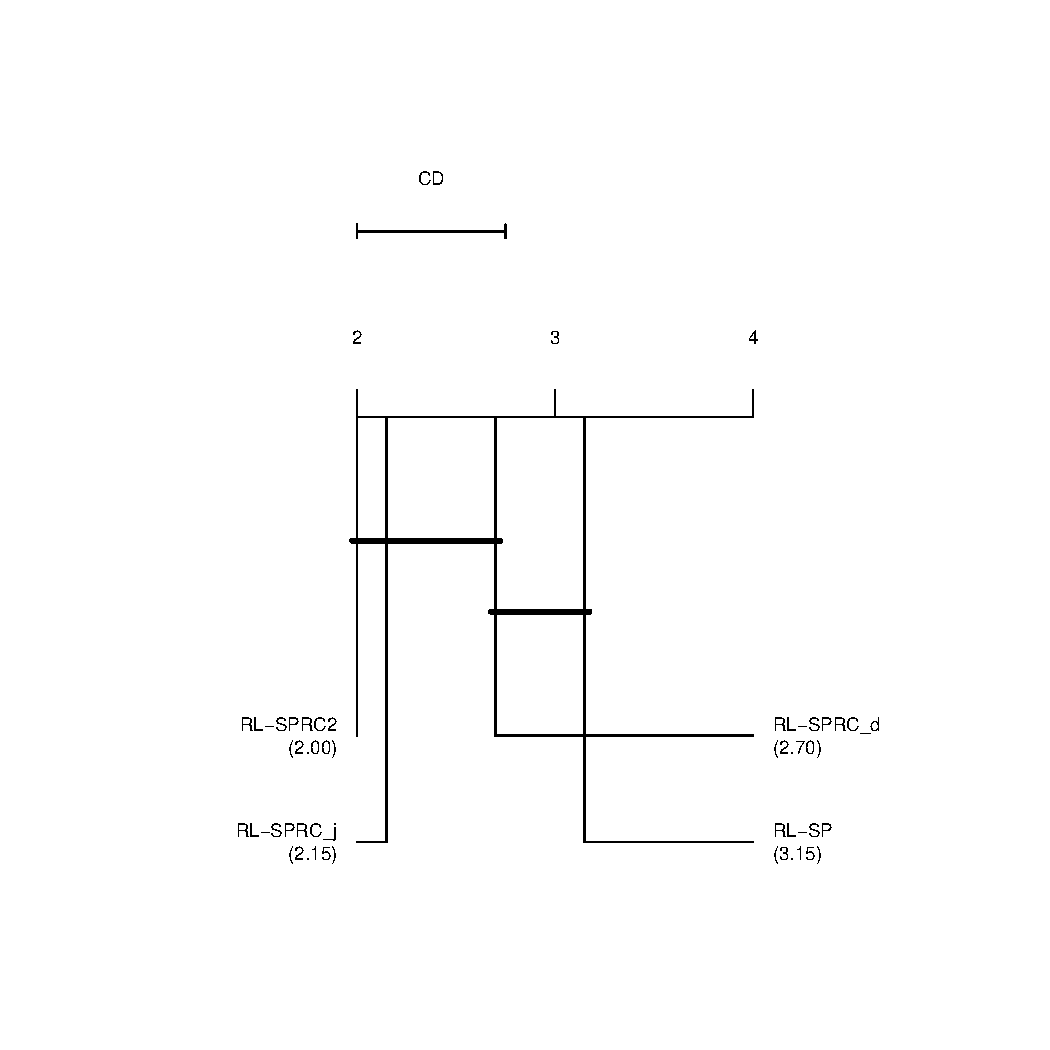
\includegraphics[scale=0.6]{imagens/rls.pdf}
        \vspace*{-2cm}
        \caption{ID = 7.81, VC = 2.68, DC = 0.74}
    \end{subfigure}
    \caption{Testes  de  Iman-Davenport  e   Nemenyi  para  as
diferentes RLs}
    \label{fig:rl-nemenyi}
\end{figure}

Por serem  estatisticamente equivalentes,  no procedimento para  selecionar qual
dentre as  três relaxações é  considerada melhor,  pode-se analisar o  número de
vitórias para cada relaxação, como apresentado na Tabela \ref{tab:contagem-rls}.
A primeira  linha e  coluna referenciam  as relaxações,  cada posição  da tabela
representa o número de vitórias da abordagem referente a linha sobre a abordagem
na coluna.

\begin{table}[!ht]
\centering
\resizebox{\textwidth}{!}{%
\begin{tabular}{llclclclc}
\hline
\multicolumn{1}{c}{Relaxações} & \multicolumn{1}{c}{} & RL-SP & \multicolumn{1}{c}{} & RL-SPRC$_{\lambda}$ & \multicolumn{1}{c}{} & RL-SPRC$_{\xi}$ & \multicolumn{1}{c}{} & RL-SPRC2 \\ \hline
RL-SP &  & - &  & 04 &  & 00 &  & 02 \\
RL-SPRC$_{\lambda}$ &  & 15 &  & - &  & 04 &  & 01 \\
RL-SPRC$_{\xi}$ &  & 22 &  & 14 &  & - &  & 05 \\
RL-SPRC2 &  & 21 &  & 18 &  & 09 &  & - \\ \hline
\end{tabular}%
}
\caption{Contagem de vitórias entre as RLs.}
\label{tab:contagem-rls}
\end{table}

Pela contagem  de vitórias,  observa-se que a  relaxação {\rlq}  teve desempenho
superior  as outras  duas  em uma  quantidade maior  de  instâncias. Enquanto  a
relaxação {\rlu}  obteve os  piores \textit{ranks}  médios e  o menor  número de
vitórias em comparação com demais relaxações. É possível inferir que a qualidade
dos  \gls{ls}s  obtidos com  a  aplicação  da  heurística  de busca  local  está
fortemente  atrelada  com a  qualidade  dos  caminhos  gerados pela  solução  do
\gls{ppl}, pois o  pior \textit{rank} médio está associado com  a relaxação mais
fraca, que por sua vez resulta em um \gls{ppl} cuja solução é menos interessante
do ponto de vista heurístico. A relaxação  contendo maior número de vitórias e o
melhor  \textit{rank} médio,  para  esse  conjunto de  instâncias,  se trata  da
{\rlq}, na  qual o \gls{ppl}  tem a  maior complexidade computacional  dentre as
relaxações propostas.

\section{BRKGA}

Na  implementação  dos  decodificadores  para o  \gls{brkga},  foi  utilizada  a
biblioteca Boost  C++ na versão 1.73  para computar a \gls{agm}.  O tempo máximo
para resolução de cada instância foi pré-definido com valor de 1800 segundos (30
minutos). Os valores de parâmetros utilizados no \gls{brkga} foram empiricamente
validados e consistem em:

\begin{itemize}
\item \textbf{População:} são geradas três populações independentes contendo 500
indivíduos cada uma.  O conjunto de elite  é formado por $10\%$  da população. A
cada iteração, $5\%$ dos indivíduos da população são substituídos por mutantes;
\item  \textbf{\textit{Crossover}:}  um novo  indivíduo  é  gerado a  partir  do
cruzamento de  dois indivíduos da  geração atual, um do  conjunto elite e  um do
conjunto não elite. Sendo 70$\%$ de probabilidade do filho herdar o alelo do pai
do conjunto de elite.
\item  \textbf{Gerações:} o  número máximo  de  gerações foi  limitada em  1000,
efetuando a troca dos 2 melhores indivíduos a cada 100 gerações.
\end{itemize}

As  versões do  \gls{brkga} nesta  seção são  diferenciadas principalmente  pela
função de aptidão utilizada (F1, F2 ou F3), mas são consideradas características
adicionais  ao decodificador  como a  adição do  procedimento de  \gls{bl} ou  a
alteração  no  procedimento  de  geração  das  chaves  aleatórias  com  base  na
frequência dos arcos da relaxação lagrangiana (RL).

A  Tabela \ref{tab:brkga-resultados}  contém  os resultados  de  5 variações  do
\gls{brkga}, as duas primeiras  com função de aptidão F1 (``F1'')  e a função de
aptidão F2 (``F2''). A função de aptidão  F3 é utilizada nas 3 outras variações,
respectivamente (``F3''), (``F3-BL'')  e (``F3-RL''). As primeiras  4 colunas da
tabela apresentam,  respectivamente, o nome  da instância, quantidade de  nós do
grafo  (``|V|''), número  de nós  terminais (``|D|'')  e a  quantidade de  arcos
(``|A|''). Para  cada algoritmo  são dispostas duas  colunas: ``LS''  contendo o
número  de terminais  atendidos  na  melhor solução  e  a  coluna ``Tempo''  que
apresenta o tempo de execução em segundos. O valor TLE representa que a execução
atingiu o tempo  limite de execução. Valores em  \textbf{negrito} representam os
melhores \gls{ls}s dentre as versões do \gls{brkga} para cara instância. A linha
``\textbf{Melhor}'' indica o número de instâncias nas quais o algoritmo obteve a
melhor  solução e  que nenhuma  outra variação  atingiu o  mesmo valor.  A linha
``\textbf{Igual}'' contém  o número  de instâncias cujo  limitante foi  igual ao
melhor obtido entre  as demais versões. A linha  ``\textbf{Pior}'' contabiliza o
total  de casos  onde a  solução retornada  pelo decodificador  foi inferior  ao
melhor limitante para a instância.

\newpage

\begin{table}[!ht]
\centering
\resizebox{\textwidth}{!}{%
\begin{tabular}{lrrrrrrrrrrrrrrrrr}
\hline
\multicolumn{1}{c}{\textbf{}} & \multicolumn{1}{c}{\textbf{}} & \multicolumn{1}{c}{\textbf{}} & \multicolumn{1}{c}{\textbf{}} & \multicolumn{2}{c}{\textbf{F1}} & \multicolumn{1}{c}{\textbf{}} & \multicolumn{2}{c}{\textbf{F2}} & \multicolumn{1}{c}{\textbf{}} & \multicolumn{2}{c}{\textbf{F3}} & \multicolumn{1}{c}{\textbf{}} & \multicolumn{2}{c}{\textbf{F3-BL}} & \multicolumn{1}{c}{\textbf{}} & \multicolumn{2}{c}{\textbf{F3-RL}} \\ \cline{5-6} \cline{8-9} \cline{11-12} \cline{14-15} \cline{17-18} 
\multicolumn{1}{c}{\textbf{Instância}} & \multicolumn{1}{c}{\textbf{|V|}} & \multicolumn{1}{c}{\textbf{|D|}} & \multicolumn{1}{c}{\textbf{|E|}} & \multicolumn{1}{c}{\textbf{LS}} & \multicolumn{1}{c}{\textbf{Tempo}} & \multicolumn{1}{c}{\textbf{}} & \multicolumn{1}{c}{\textbf{LS}} & \multicolumn{1}{c}{\textbf{Tempo}} & \multicolumn{1}{c}{\textbf{}} & \multicolumn{1}{c}{\textbf{LS}} & \multicolumn{1}{c}{\textbf{Tempo}} & \multicolumn{1}{c}{\textbf{}} & \multicolumn{1}{c}{\textbf{LS}} & \multicolumn{1}{c}{\textbf{Tempo}} & \multicolumn{1}{c}{\textbf{}} & \multicolumn{1}{c}{\textbf{LS}} & \textbf{Tempo} \\ \hline
washington-50-10-6 & 10 & 6 & 23 & \textbf{1} & 105 &  & \textbf{1} & 108 &  & \textbf{1} & 115 &  & \textbf{1} & 138 &  & \textbf{1} & 191 \\
washington-50-20-11 & 20 & 11 & 92 & \textbf{4} & 328 &  & \textbf{4} & 339 &  & \textbf{4} & 354 &  & \textbf{4} & 399 &  & \textbf{4} & 587 \\
washington-50-30-15 & 30 & 15 & 210 & \textbf{3} & 697 &  & \textbf{3} & 829 &  & \textbf{3} & 829 &  & \textbf{3} & 1.002 &  & \textbf{3} & 1347 \\
washington-50-40-23 & 40 & 23 & 415 & \textbf{6} & 1.453 &  & 7 & TLE &  & \textbf{6} & 1.688 &  & \textbf{6} & 1.651 &  & \textbf{6} & 1683 \\
washington-50-50-28 & 50 & 28 & 624 & \textbf{13} & TLE &  & \textbf{13} & TLE &  & \textbf{13} & TLE &  & \textbf{13} & TLE &  & \textbf{13} & TLE \\
washington-50-60-35 & 60 & 35 & 906 & \textbf{17} & TLE &  & 19 & TLE &  & \textbf{17} & TLE &  & 18 & TLE &  & \textbf{17} & TLE \\
washington-50-70-37 & 70 & 37 & 1258 & \textbf{16} & TLE &  & 18 & TLE &  & \textbf{16} & TLE &  & 17 & TLE &  & \textbf{16} & TLE \\
washington-50-80-39 & 80 & 39 & 1796 & \textbf{29} & TLE &  & \textbf{29} & TLE &  & \textbf{29} & TLE &  & \textbf{29} & TLE &  & \textbf{29} & TLE \\
washington-50-90-51 & 90 & 51 & 2109 & \textbf{36} & TLE &  & \textbf{36} & TLE &  & \textbf{36} & TLE &  & \textbf{36} & TLE &  & \textbf{36} & TLE \\
washington-50-100-45 & 100 & 45 & 2208 & 35 & TLE &  & 35 & TLE &  & \textbf{34} & TLE &  & \textbf{34} & TLE &  & \textbf{34} & TLE \\ \hline
washington-75-10-4 & 10 & 4 & 16 & \textbf{3} & 144 &  & \textbf{3} & 147 &  & \textbf{3} & 100 &  & \textbf{3} & 148 &  & \textbf{3} & 152 \\
washington-75-20-12 & 20 & 12 & 63 & 5 & 413 &  & \textbf{4} & 388 &  & \textbf{4} & 338 &  & \textbf{4} & 513 &  & \textbf{4} & 468 \\
washington-75-30-16 & 30 & 16 & 159 & \textbf{5} & 935 &  & \textbf{5} & 794 &  & \textbf{5} & 742 &  & \textbf{5} & 897 &  & \textbf{5} & 740 \\
washington-75-40-21 & 40 & 21 & 269 & \textbf{5} & 1.127 &  & 8 & 1.172 &  & 6 & 1.228 &  & 6 & 1.351 &  & \textbf{5} & 1183 \\
washington-75-50-30 & 50 & 30 & 438 & \textbf{11} & TLE &  & \textbf{11} & 1.707 &  & \textbf{11} & TLE &  & \textbf{11} & TLE &  & \textbf{11} & TLE \\
washington-75-60-25 & 60 & 25 & 628 & \textbf{11} & TLE &  & 12 & TLE &  & \textbf{11} & TLE &  & \textbf{11} & TLE &  & \textbf{11} & TLE \\
washington-75-70-42 & 70 & 42 & 850 & 23 & TLE &  & 16 & TLE &  & \textbf{13} & TLE &  & \textbf{13} & TLE &  & \textbf{13} & TLE \\
washington-75-80-48 & 80 & 48 & 1252 & 29 & TLE &  & 26 & TLE &  & 13 & TLE &  & \textbf{11} & TLE &  & 13 & TLE \\
washington-75-90-47 & 90 & 47 & 1517 & \textbf{19} & TLE &  & \textbf{19} & TLE &  & \textbf{19} & TLE &  & \textbf{19} & TLE &  & \textbf{19} & TLE \\
washington-75-100-52 & 100 & 52 & 1896 & 28 & TLE &  & 33 & TLE &  & 27 & TLE &  & 28 & TLE &  & \textbf{26} & TLE \\ \hline
washington-100-10-6 & 10 & 6 & 9 & \textbf{2} & 94 &  & \textbf{2} & 95 &  & \textbf{2} & 104 &  & \textbf{2} & 89 &  & \textbf{2} & 105 \\
washington-100-20-10 & 20 & 10 & 49 & \textbf{2} & 272 &  & \textbf{2} & 359 &  & \textbf{2} & 379 &  & \textbf{2} & 285 &  & \textbf{2} & 334 \\
washington-100-30-12 & 30 & 12 & 103 & \textbf{2} & 401 &  & \textbf{2} & 569 &  & \textbf{2} & 573 &  & \textbf{2} & 444 &  & \textbf{2} & 433 \\
washington-100-40-18 & 40 & 21 & 211 & \textbf{4} & 833 &  & \textbf{4} & TLE &  & \textbf{4} & 1.004 &  & \textbf{4} & 1.337 &  & \textbf{4} & 1278 \\
washington-100-50-27 & 50 & 27 & 298 & \textbf{9} & 1.147 &  & \textbf{9} & TLE &  & \textbf{9} & 1.666 &  & \textbf{9} & 1.485 &  & \textbf{9} & TLE \\
washington-100-60-34 & 60 & 34 & 427 & \textbf{10} & 1.620 &  & 11 & TLE &  & \textbf{10} & TLE &  & \textbf{10} & TLE &  & \textbf{10} & TLE \\
washington-100-70-39 & 70 & 39 & 602 & \textbf{24} & TLE &  & \textbf{24} & TLE &  & \textbf{24} & TLE &  & \textbf{24} & TLE &  & \textbf{24} & TLE \\
washington-100-80-32 & 80 & 32 & 882 & 18 & TLE &  & 7 & TLE &  & \textbf{6} & TLE &  & \textbf{6} & TLE &  & \textbf{6} & TLE \\
washington-100-90-43 & 90 & 43 & 1151 & 32 & TLE &  & 20 & TLE &  & \textbf{11} & TLE &  & 13 & TLE &  & \textbf{11} & TLE \\
washington-100-100-43 & 100 & 43 & 1408 & 14 & TLE &  & 13 & TLE &  & \textbf{12} & TLE &  & \textbf{12} & TLE &  & \textbf{12} & TLE \\ \hline
washington-200-125-55 & 125 & 55 & 1224 & 42 & TLE &  & 42 & TLE &  & \textbf{32} & TLE &  & 33 & TLE &  & 33 & TLE \\
washington-200-150-61 & 150 & 61 & 2234 & 41 & TLE &  & 44 & TLE &  & 37 & TLE &  & 37 & TLE &  & \textbf{35} & TLE \\
washington-200-175-74 & 175 & 74 & 3024 & 39 & TLE &  & 42 & TLE &  & 40 & TLE &  & \textbf{38} & TLE &  & 39 & TLE \\
washington-200-200-114 & 200 & 114 & 3645 & 105 & TLE &  & 105 & TLE &  & 88 & TLE &  & 89 & TLE &  & \textbf{75} & TLE \\
washington-200-225-135 & 225 & 135 & 4464 & 79 & TLE &  & 87 & TLE &  & 65 & TLE &  & 73 & TLE &  & \textbf{62} & TLE \\
washington-200-250-109 & 250 & 109 & 6403 & 76 & TLE &  & 83 & TLE &  & 61 & TLE &  & 61 & TLE &  & \textbf{55} & TLE \\
washington-200-275-146 & 275 & 146 & 7195 & 109 & TLE &  & 116 & TLE &  & 104 & TLE &  & 103 & TLE &  & \textbf{101} & TLE \\
washington-200-300-136 & 300 & 136 & 8709 & 116 & TLE &  & 116 & TLE &  & 102 & TLE &  & 100 & TLE &  & \textbf{99} & TLE \\
washington-200-325-170 & 325 & 170 & 9260 & 151 & TLE &  & 154 & TLE &  & 135 & TLE &  & 130 & TLE &  & \textbf{128} & TLE \\
washington-200-350-150 & 350 & 150 & 12218 & 124 & TLE &  & 127 & TLE &  & 98 & TLE &  & 97 & TLE &  & \textbf{96} & TLE \\ \hline
\multicolumn{1}{l}{\textbf{Melhor}} &  &  &  & 0 &  &  & 0 &  &  & 1 &  &  & 2 &  &  & 9 &  \\
\multicolumn{1}{l}{\textbf{Igual}} &  &  &  & 22 &  &  & 17 &  &  & 27 &  &  & 24 &  &  & 28 &  \\
\multicolumn{1}{l}{\textbf{Pior}} &  &  &  & 18 &  &  & 23 &  &  & 12 &  &  & 14 &  &  & 3 &  \\ \hline
\end{tabular}%
}
\caption{Resultados das versões do BRKGA.}
\label{tab:brkga-resultados}
\end{table}

\begin{comment}
Inicialmente para investigar o desempenho das diferentes versões do \gls{brkga} para o conjunto de instâncias, foi utilizado o teste de Iman-Davenport e quando uma diferença estatisticamente significativa (DES) é identificada por esse teste, procedemos com o teste de Nemenyi para detectar grupos de heurísticas equivalentes entre si. Para todos os testes consideramos um nível de confiança de $95\%$, com a hipótese nula de que não existe DES entre todas as heurísticas.

Considerando os valores de \gls{ls} constantes na Tabela \ref{tab:brkga-resultados}, os seguintes resultados foram computados:
\begin{itemize}
    \item O valor de \textit{rank} médio das versões, em ordem crescente, é:
        \begin{itemize}
            \item F3-RL = 2.24
            \item F3 = 2.64
            \item F3-BL = 2.69
            \item F1 = 3.48
            \item F2 = 3.96
        \end{itemize}
    \item Valor de teste de Iman-Davenport = $9.52$;
    \item De acordo com a distribuição, o Valor Crítico = $2.42$;
    \item Segundo o teste de Nemenyi, o valor de Diferença Crítica = $0.97$.
\end{itemize}
\end{comment}

Considerando  os resultados  da  Tabela  \ref{tab:brkga-resultados}, nota-se  um
consumo de tempo  relativamente alto dos decodificadores  independente de função
de aptidão, dado que quase todas as  instâncias contendo 50 ou mais nós, não foi
possível  executar o  \gls{brkga} por  1000 gerações  antes de  atingir o  tempo
limite de 30 minutos. A quantidade de TLEs de cada algoritmo foi bem semelhante,
sendo  {\bfum} a  versão com  menos TLEs,  totalizando 26.  Em contrapartida,  a
versão  {\bfdois} tem  o maior  número  de instâncias  onde o  tempo limite  foi
alcançado, totalizando  29 casos.  O tempo  médio para as  instâncias em  que os
\gls{brkga}s executaram  por 1000 gerações,  se manteve  entre 10 e  12 minutos,
para todas as versões.

A aplicação  do teste  de Iman-Davenport  indicou a existência  de DES  entre as
amostras. Ao aplicar o teste de Nemenyi o resultado agrupou as versões F3, F3-BL
e F3-RL com  os menores valores de  {\em rank} médio, o  que indica equivalência
estatística. Esses dados estão  representados na Figura \ref{fig:brkga-nemenyi},
que também contém o valor computado pelos testes de Iman-Davenport (ID), o Valor
Crítico (VC) e a Diferença Crítica (DC). \newline

%\vspace*{-1.8cm}
\begin{figure}[!ht]
    \centering
    \begin{subfigure}{.5\textwidth}
        \centering
        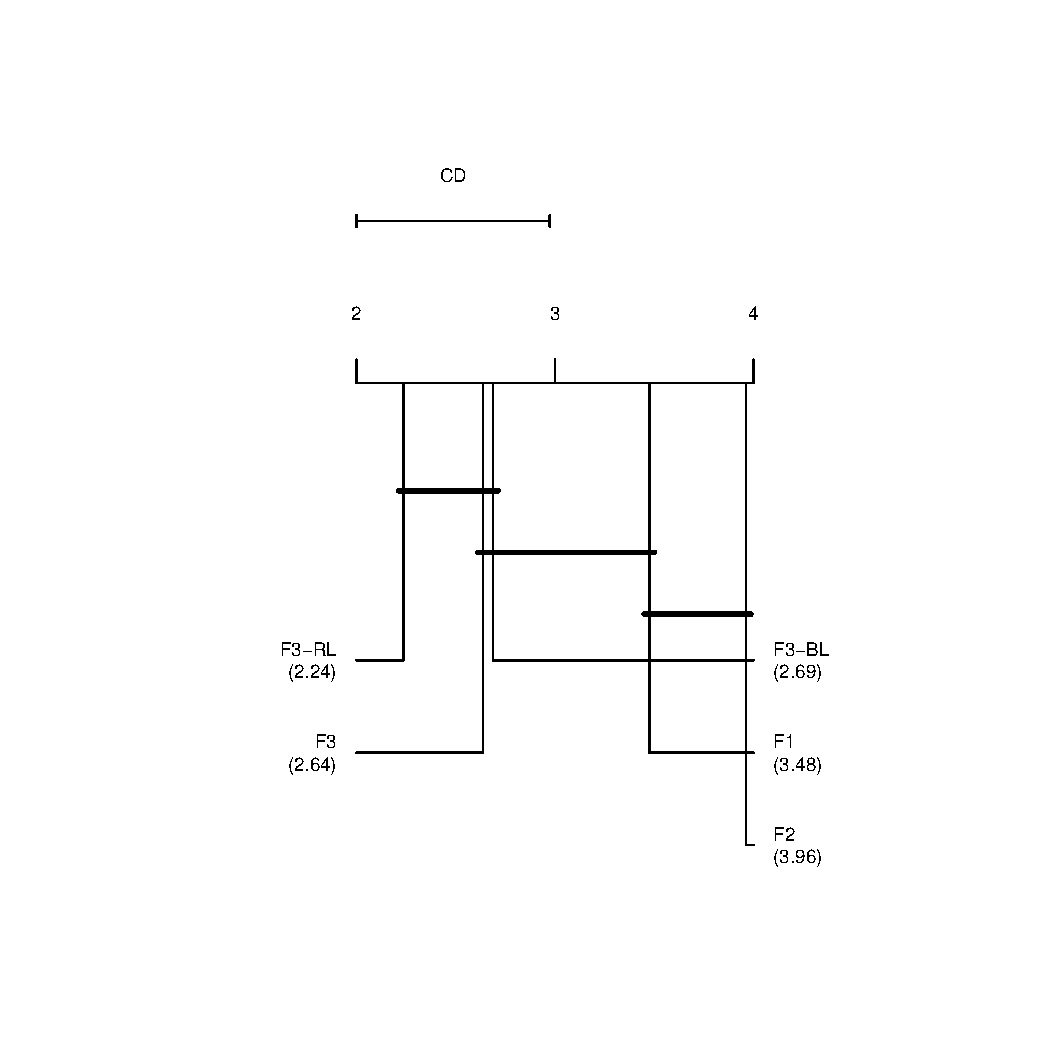
\includegraphics[scale=0.6]{imagens/plot-id.pdf}
        \vspace*{-2cm}
        \caption{ID = 9.52, VC = 2.42, DC = 0.97}
    \end{subfigure}
    \caption{Testes de Imand-Davenport e Nemenyi para os
      decodificadores das versões do BRKGA.}
    \label{fig:brkga-nemenyi}
\end{figure}

Entretanto, ao notar a diferença de {\em rank} médio entre os \gls{brkga}s F3-RL
e F3, optou-se  pela aplicação do teste estatístico de  Wilcoxon para essas duas
variações, motivado pelo fato desse teste estatístico apresentar resultados mais
confiáveis tratando-se apenas de duas amostras. O resultado calculado pelo teste
de Wilcoxon foi $-5.47$, o que significa que existe DES entre as abordagens. Por
fim, além da  diferença estatística, a contagem de vitórias  da versão F3-RL foi
maior, possibilitando  afirmar que  essa versão pode  ser considerada  melhor em
comparação com as demais variações do \gls{brkga}.

Considerando a  capacidade de melhora  das soluções,  é possível observar  que a
versão {\bfdois}, que utiliza a abordagem de soma das penalizações, foi a função
de  aptidão  que  apresentou  os   piores  resultados  dentre  as  5  abordagens
comparadas.  Dentre  as  versões  do   \gls{brkga}  que  obtiveram  os  melhores
resultados, mais especificamente as variações  da função F3, nenhuma dominou por
completo as demais abordagens, ou seja,  não houve um algoritmo cujos resultados
foram melhores em todas as 40 instâncias.

A utilização da busca local não apresentou ganhos significativos, obtendo apenas
6 soluções  melhores que a versão  {\bftres} sem utilizar busca  local, enquanto
gerou  resultados  inferiores   para  outras  7  instâncias.  Já   a  versão  do
decodificador  F3-RL apresentou  \gls{ls}s  com a  maior  qualidade, gerando  as
melhores  soluções para  37 instâncias.  Para as  outras 3  instâncias em  que o
melhor  valor foi  obtido exclusivamente  por  outra versão,  a diferença  entre
resultados foi menor ou igual a 2 terminais. Tais resultados reafirmam a melhora
de qualidade das soluções com base na utilização da informação de frequência dos
arcos selecionados pelo \gls{ppl} na relaxação {\rlq}$^C$.


% k = numero heuristicas
% N = numero de instancias
% Iman-Davenport = 9.52 ($F_f$)
% Valor Crítico = 2.42
% Como o valor encontrado pelo teste ff é maio que o valor crítico, podemos rejeitar a hipótese nula.
% Teste de Nemenyi para computar a diferença crítica e identificar quais grupos de heurísticas que são estatisticamente equivalentes entre si.
% Wilcoxon z < −1.96, podemos rejeitar a hipótese nula.
% Wilcoxon(F3-BL, F3-RL) = -5.47
% Diferença crítica = 0.97 

\newpage

\section{Avaliação Geral dos Limitantes Inferiores} \label{sec:resultados-li}

Esta seção  apresenta a comparação  de todos \gls{li}s obtidos  pelas abordagens
propostas neste  trabalho. Para  tal, serão  considerados os  melhores \gls{li}s
obtidos  pelos modelos  \gls{dmfm-pma}  e \gls{ab-pma},  juntamente dos  valores
retornados por suas respectivas relaxações  lineares e os melhores \gls{li}s das
\gls{rl}s.

A Tabela  \ref{tab:lis-all-comp} contém  os \gls{li}s das  melhores metodologias
utilizadas   nesta   dissertação.   As    primeiras   quatro   colunas   contém,
respectivamente, o  nome da  instância, o  número de nós  do grafo  (``|V|''), a
quantidade de nós terminais (``|D|'') e  o número de arcos (``|A|''). As colunas
subsequentes  dividem-se entre  as  abordagens, indicando  o  valor de  \gls{li}
obtido  (``LI'') e  o  tempo de  execução em  segundos  (``Tempo''). As  colunas
``\gls{dmfm-pma}'' e  ``\gls{ab-pma}'' apresentam, respectivamente,  os melhores
limitantes     retornados    pelo     resolvedor    \gls{pli}.     As    colunas
``\gls{dmfm-pma}$_{lin}$''  e  ``\gls{ab-pma}$_{lin}$''  contém  as  respectivas
relaxações  lineares  dos  modelos.  A   última  coluna  apresenta  os  melhores
resultados  da  relaxação {\rlq},  dado  que  esta  \gls{rl} detém  os  melhores
\gls{li}s dentre todas as variações.

\begin{table}[!ht]
\centering
\resizebox{\textwidth}{!}{%
\begin{tabular}{lrrrlrrlrrlrrlrrlrr}
\hline
\multicolumn{1}{c}{} & \multicolumn{1}{c}{} & \multicolumn{1}{c}{} & \multicolumn{1}{c}{} & \multicolumn{1}{c}{} & \multicolumn{2}{c}{\textbf{DMFM-MRP}} & \multicolumn{1}{c}{} & \multicolumn{2}{c}{\textbf{AB-MRP}} & \multicolumn{1}{c}{} & \multicolumn{2}{c}{\textbf{DMFM-MRP$_{lin}$}} & \multicolumn{1}{c}{\textbf{}} & \multicolumn{2}{c}{\textbf{AB-MRP$_{lin}$}} & \multicolumn{1}{c}{\textbf{}} & \multicolumn{2}{c}{\textbf{RL-SPRC2}} \\ \cline{6-7} \cline{9-10} \cline{12-13} \cline{15-16} \cline{18-19} 
\multicolumn{1}{c}{\textbf{Instância}} & \multicolumn{1}{c}{\textbf{|V|}} & \multicolumn{1}{c}{\textbf{|D|}} & \multicolumn{1}{c}{\textbf{|A|}} & \multicolumn{1}{c}{\textbf{}} & \multicolumn{1}{c}{\textbf{LI}} & \multicolumn{1}{c}{\textbf{Tempo}} & \multicolumn{1}{c}{} & \multicolumn{1}{c}{\textbf{LI}} & \multicolumn{1}{c}{\textbf{Tempo}} & \multicolumn{1}{c}{} & \multicolumn{1}{c}{\textbf{LI}} & \multicolumn{1}{c}{\textbf{Tempo}} & \multicolumn{1}{c}{\textbf{}} & \multicolumn{1}{c}{\textbf{LI}} & \multicolumn{1}{c}{\textbf{Tempo}} & \multicolumn{1}{c}{\textbf{}} & \multicolumn{1}{c}{\textbf{LI}} & \multicolumn{1}{c}{\textbf{Tempo}} \\ \hline
washington-50-10-6 & 10 & 6 & 46 &  & \textbf{1} & 0,0 &  & \textbf{1} & 0,0 &  & \textbf{1} & 0,0 &  & 0 & 0,0 &  & \textbf{1} & 0 \\
washington-50-20-11 & 20 & 11 & 184 &  & \textbf{4} & 0,0 &  & \textbf{4} & 0,0 &  & 3 & 0,1 &  & 0 & 0,0 &  & 3 & 34 \\
washington-50-30-15 & 30 & 15 & 420 &  & \textbf{3} & 0,0 &  & \textbf{3} & 0,0 &  & 2 & 0,1 &  & 0 & 0,0 &  & 2 & 75 \\
washington-50-40-23 & 40 & 23 & 830 &  & \textbf{6} & 3,0 &  & \textbf{6} & 4,0 &  & 1 & 0,6 &  & 0 & 0,0 &  & 4 & 786 \\
washington-50-50-28 & 50 & 28 & 1248 &  & \textbf{13} & 3,0 &  & \textbf{13} & 1,0 &  & 7 & 1,0 &  & 0 & 0,0 &  & 6 & 345 \\
washington-50-60-35 & 60 & 35 & 1812 &  & \textbf{15} & 4,0 &  & \textbf{15} & 3,0 &  & 3 & 2,7 &  & 0 & 0,0 &  & 2 & 435 \\
washington-50-70-37 & 70 & 37 & 2516 &  & \textbf{16} & 41,0 &  & \textbf{16} & 26,0 &  & 4 & 4,9 &  & 0 & 0,0 &  & 7 & 823 \\
washington-50-80-39 & 80 & 39 & 3592 &  & \textbf{26} & 25,0 &  & \textbf{26} & 584,0 &  & 23 & 5,1 &  & 0 & 0,0 &  & 23 & 1.336 \\
washington-50-90-51 & 90 & 51 & 4218 &  & \textbf{35} & 285,0 &  & \textbf{35} & 355,0 &  & 18 & 13,4 &  & 0 & 0,0 &  & 19 & 1.790 \\
washington-50-100-45 & 100 & 45 & 4416 &  & \textbf{28} & 71,0 &  & \textbf{28} & 262,0 &  & 12 & 11,8 &  & 0 & 0,0 &  & 16 & TLE \\ \hline
washington-75-10-4 & 10 & 4 & 32 &  & \textbf{3} & 0,0 &  & \textbf{3} & 0,0 &  & 1 & 0,0 &  & 0 & 0,0 &  & 2 & 9 \\
washington-75-20-12 & 20 & 12 & 126 &  & \textbf{4} & 0,0 &  & \textbf{4} & 0,0 &  & 2 & 0,1 &  & 0 & 0,0 &  & 2 & 34 \\
washington-75-30-16 & 30 & 16 & 318 &  & \textbf{5} & 6,0 &  & \textbf{5} & 3,0 &  & 1 & 0,3 &  & 0 & 0,0 &  & 0 & 265 \\
washington-75-40-21 & 40 & 21 & 538 &  & \textbf{5} & 1,0 &  & \textbf{5} & 3,0 &  & \textbf{5} & 0,5 &  & 0 & 0,0 &  & 4 & 209 \\
washington-75-50-30 & 50 & 30 & 876 &  & \textbf{9} & 579,0 &  & \textbf{9} & 2175,0 &  & 3 & 1,0 &  & 0 & 0,0 &  & 3 & 375 \\
washington-75-60-25 & 60 & 25 & 1256 &  & \textbf{11} & 4,0 &  & \textbf{11} & 2,0 &  & 2 & 0,7 &  & 0 & 0,0 &  & 2 & 302 \\
washington-75-70-42 & 70 & 42 & 1700 &  & \textbf{12} & 19,0 &  & \textbf{12} & 136,0 &  & 6 & 5,3 &  & 0 & 0,0 &  & 6 & 856 \\
washington-75-80-48 & 80 & 48 & 2504 &  & \textbf{9} & 42,0 &  & \textbf{9} & 148,0 &  & 2 & 11,1 &  & 0 & 0,0 &  & 2 & 1.292 \\
washington-75-90-47 & 90 & 47 & 3034 &  & \textbf{19} & 89,0 &  & 10 & TLE &  & 3 & 10,7 &  & 0 & 0,0 &  & 3 & 1.448 \\
washington-75-100-52 & 100 & 52 & 3792 &  & \textbf{14} & TLE &  & 13 & TLE &  & 9 & 24,4 &  & 0 & 0,0 &  & 10 & TLE \\ \hline
washington-100-10-6 & 10 & 6 & 18 &  & \textbf{2} & 0,0 &  & \textbf{2} & 0,0 &  & \textbf{2} & 0,0 &  & 0 & 0,0 &  & \textbf{2} & 0 \\
washington-100-20-10 & 20 & 10 & 98 &  & \textbf{2} & 0,0 &  & \textbf{2} & 0,0 &  & 1 & 0,0 &  & 0 & 0,0 &  & 0 & 37 \\
washington-100-30-12 & 30 & 12 & 206 &  & \textbf{2} & 16,0 &  & \textbf{2} & 0,0 &  & 1 & 0,1 &  & 1 & 0,0 &  & \textbf{2} & 90 \\
washington-100-40-18 & 40 & 21 & 422 &  & \textbf{4} & 22,0 & \textbf{} & 4 & 5,0 &  & 1 & 0,5 &  & 0 & 0,0 &  & 1 & 298 \\
washington-100-50-27 & 50 & 27 & 596 &  & 5 & TLE &  & \textbf{9} & 121,0 &  & 1 & 2,7 &  & 0 & 0,0 &  & 1 & 0 \\
washington-100-60-34 & 60 & 34 & 854 &  & \textbf{10} & 3,0 &  & \textbf{10} & 94,0 &  & 7 & 1,2 &  & 0 & 0,0 &  & 7 & 270 \\
washington-100-70-39 & 70 & 39 & 1204 &  & \textbf{17} & 151,0 &  & \textbf{17} & 183,0 &  & 9 & 2,6 &  & 0 & 0,0 &  & 9 & 663 \\
washington-100-80-32 & 80 & 32 & 1764 &  & \textbf{5} & 11,0 &  & \textbf{5} & 23,0 &  & 4 & 3,8 &  & 0 & 0,0 &  & 3 & TLE \\
washington-100-90-43 & 90 & 43 & 2302 &  & \textbf{11} & 107,0 &  & \textbf{11} & 160,0 &  & 3 & 8,6 &  & 0 & 0,0 &  & 2 & 1.216 \\
washington-100-100-43 & 100 & 43 & 2816 &  & \textbf{4} & 146,0 &  & \textbf{4} & 157,0 &  & 2 & 17,3 &  & 0 & 0,0 &  & 1 & 1.513 \\ \hline
washington-200-125-55 & 125 & 55 & 2448 &  & \textbf{29} & 338,0 &  & 27 & TLE &  & 10 & 13,4 &  & 0 & 0,0 &  & 9 & TLE \\
washington-200-150-61 & 150 & 61 & 4468 &  & \textbf{10} & TLE &  & 2 & TLE &  & 7 & 187,4 &  & 0 & 0,1 &  & 7 & TLE \\
washington-200-175-74 & 175 & 74 & 6048 &  & \textbf{20} & TLE &  & 7 & TLE &  & 19 & 2225,4 &  & 0 & 0,1 &  & 18 & TLE \\
washington-200-200-114 & 200 & 114 & 7290 &  & \textbf{32} & TLE &  & 8 & TLE &  & 24 & 730,3 &  & 0 & 0,2 &  & 23 & TLE \\
washington-200-225-135 & 225 & 135 & 8928 &  & 2 & TLE &  & \textbf{8} & TLE &  & 0 & TLE &  & 0 & 0,2 &  & 2 & TLE \\
washington-200-250-109 & 250 & 109 & 12806 &  & 6 & TLE &  & \textbf{11} & TLE &  & 0 & TLE &  & 0 & 0,2 &  & 6 & TLE \\
washington-200-275-146 & 275 & 146 & 14390 &  & \textbf{11} & TLE &  & \textbf{11} & TLE &  & 0 & TLE &  & 0 & 0,2 &  & \textbf{11} & TLE \\
washington-200-300-136 & 300 & 136 & 17418 &  & - & TLE &  & 2 & TLE &  & 0 & TLE &  & 1 & 0,3 &  & \textbf{10} & TLE \\
washington-200-325-170 & 325 & 170 & 18520 &  & - & TLE &  & \textbf{16} & TLE &  & 0 & TLE &  & 0 & 0,4 &  & 13 & TLE \\
washington-200-350-150 & 350 & 150 & 24436 &  & - & TLE &  & \textbf{4} & TLE &  & 0 & TLE &  & 0 & 0,4 &  & \textbf{4} & TLE \\ \hline
\end{tabular}%
}
\caption{Comparação dos melhores LIs entre as metodologias.}
\label{tab:lis-all-comp}
\end{table}

A  aplicação do  teste  de  Iman-Davenport nos  valores  apresentados na  Tabela
\ref{tab:lis-all-comp},  indicou a  presença de  DES entre  as amostras.  Assim,
aplicando  o teste  de  Nemenyi agruparam-se,  com menor  {\em  rank} médio,  os
resultados dos modelos \gls{dmfm-pma} e  \gls{ab-pma}, o que indica equivalência
estatística.     Esses      dados     estão     representados      na     Figura
\ref{fig:all-lis-nemenyi}, que também  contém o valor computado  pelos testes de
Iman-Davenport (ID), o Valor Crítico (VC)  e a Diferença Crítica (DC). Até mesmo
a contagem de  vitórias nos modelos foi igual: cada  um contabilizou 6 vitórias,
enquanto os \gls{li}s foram iguais para as outras 28 instâncias. Ainda assim, os
resultados  dos modelos  não  dominaram  as demais  metodologias  para todas  as
instâncias, ou seja, alguma outra  metodologia apresentou pelo menos um \gls{li}
melhor que ambos os modelos.

\begin{figure}[!ht]
    \centering
    \begin{subfigure}{.5\textwidth}
        \centering
        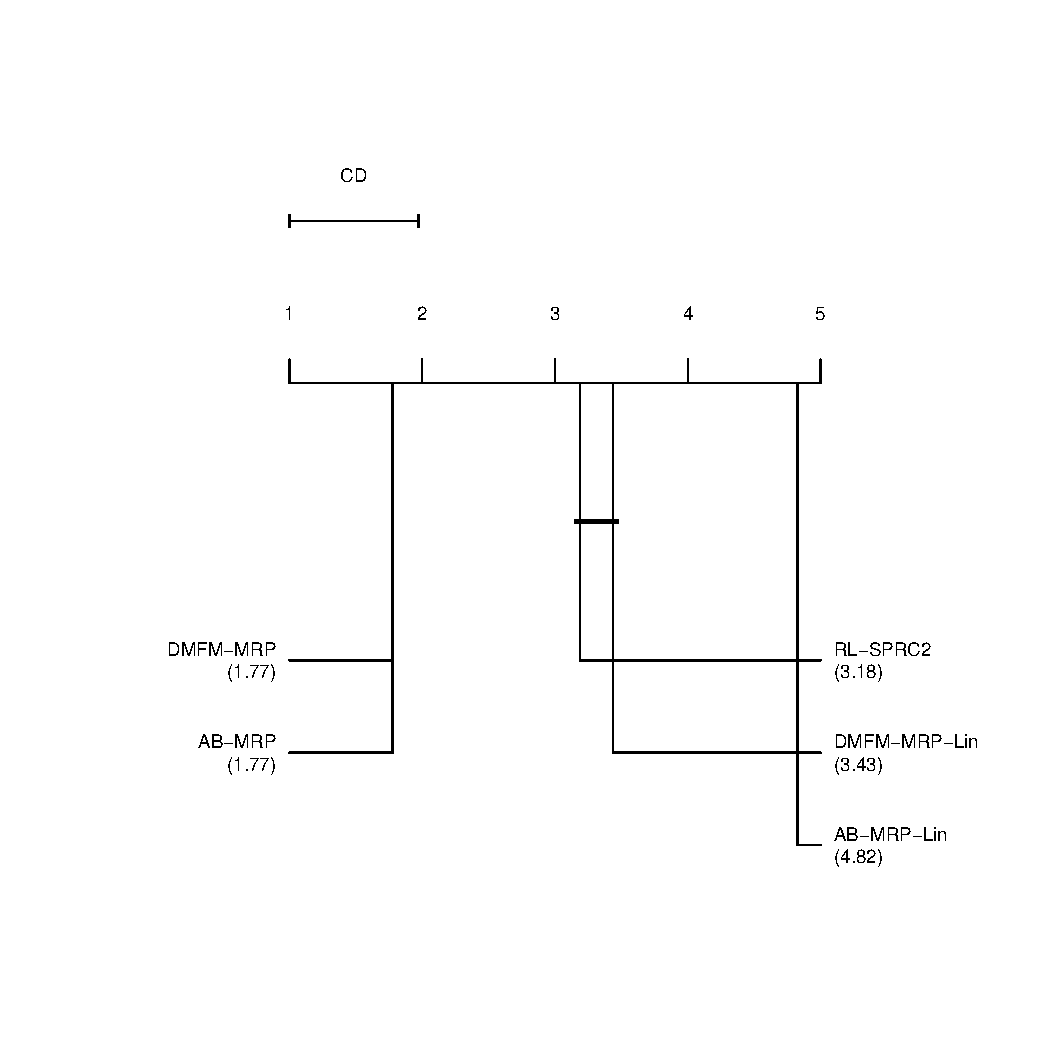
\includegraphics[scale=0.6]{imagens/lis-all.pdf}
        \vspace*{-2cm}
        \caption{ID = 74.32, VC = 2.42, DC = 0.97}
    \end{subfigure}
    \caption{Testes de Iman-Davenport e Nemenyi para os Limitantes Inferiores.}
    \label{fig:all-lis-nemenyi}
\end{figure}

Analisando as  relaxações lineares e a  \gls{rl}, tornou-se evidente a  falta de
qualidade dos limitantes obtidos pela relaxação linear do modelo \gls{ab-pma}. O
valor da relaxação do \gls{ab-pma} para 38 instâncias foi igual a 0 e nas outras
duas instâncias, o resultado foi 1.  A relaxação linear do modelo \gls{dmfm-pma}
apresentou  melhor qualidade,  sendo  estatisticamente  equivalente à  relaxação
{\rlq}.  Entretanto, ao  considerar  a  contagem de  vitórias  entre essas  duas
abordagens, pode-se assumir que {\rlq}  foi melhor. Dado que {\rlq} contabilizou
vitória em 13  instâncias e {\gls{dmfm-pma}$_{lin}$} em apenas 11.  Com base nos
resultados e análises apresentados, notou-se  o excelente desempenho dos modelos
matemáticos, de modo que eles detém os melhores \gls{li}s para 39 instâncias.

\section{Avaliação Geral dos Limitantes Superiores} \label{sec:resultados-li}

Esta seção apresenta a comparação de todos os \gls{ls}s obtidos pelas diferentes
abordagens propostas  nesse trabalho. Para  tal, serão considerados  os melhores
\gls{ls}s  dos   modelos  \gls{dmfm-pma},  \gls{ab-pma},  a   melhor  versão  do
\gls{brkga} e da \gls{rl}.

A Tabela \ref{tab:ls-all-comp} apresenta  os \gls{ls}s das melhores metodologias
utilizadas   nesta   dissertação.   As    primeiras   quatro   colunas   contém,
respectivamente, o  nome da  instância, o  número de nós  do grafo  (``|V|''), a
quantidade de nós terminais (``|D|'') e  o número de arcos (``|A|''). As colunas
subsequentes  dividem-se entre  as  abordagens, indicando  o  valor de  \gls{ls}
(``LS'')  obtido e  o  tempo de  execução em  segundos  (``Tempo''). As  colunas
``\gls{dmfm-pma}''  e  ``\gls{ab-pma}''  contém,  respectivamente,  os  melhores
\gls{ls}  retornados  pelo  resolvedor  \gls{pli} para  cada  modelo.  A  coluna
``{\rlq}''  contém os  resultados associados  com a  \gls{rl} que  apresentou os
melhores  resultados. Por  fim,  a coluna  ``BRKGA-F3-RL''  dispõe os  \gls{ls}s
retornados pela melhor versão do \gls{brkga}.

\begin{table}[!ht] \centering \resizebox{\textwidth}{!}{%
\begin{tabular}{lrrrlrrlrrlrrlrr}
\hline
\multicolumn{1}{c}{\textbf{}} & \multicolumn{1}{c}{\textbf{}} & \multicolumn{1}{c}{\textbf{}} & \multicolumn{1}{c}{\textbf{}} & \multicolumn{1}{c}{\textbf{}} & \multicolumn{2}{c}{\textbf{DMFM-MRP}} & \multicolumn{1}{c}{\textbf{}} & \multicolumn{2}{c}{\textbf{AB-MRP}} & \multicolumn{1}{c}{\textbf{}} & \multicolumn{2}{c}{\textbf{RL-CRSP2}} & \multicolumn{1}{c}{\textbf{}} & \multicolumn{2}{c}{\textbf{BRKGA-F3-RL}} \\ \cline{6-7} \cline{9-10} \cline{12-13} \cline{15-16} 
\multicolumn{1}{c}{\textbf{Instância}} & \multicolumn{1}{c}{\textbf{|V|}} & \multicolumn{1}{c}{\textbf{|D|}} & \multicolumn{1}{c}{\textbf{|A|}} & \multicolumn{1}{c}{\textbf{}} & \multicolumn{1}{c}{\textbf{LS}} & \multicolumn{1}{c}{\textbf{Tempo}} & \multicolumn{1}{c}{\textbf{}} & \multicolumn{1}{c}{\textbf{LS}} & \multicolumn{1}{c}{\textbf{Tempo}} & \multicolumn{1}{c}{\textbf{}} & \multicolumn{1}{c}{\textbf{LS}} & \multicolumn{1}{c}{\textbf{Tempo}} & \multicolumn{1}{c}{\textbf{}} & \multicolumn{1}{c}{\textbf{LS}} & \multicolumn{1}{c}{\textbf{Tempo}} \\ \hline
washington-50-10-6 & 11 & 6 & 46 &  & \textbf{1} & 0 &  & \textbf{1} & 0 &  & \textbf{1} & 9 &  & \textbf{1} & 191 \\
washington-50-20-11 & 21 & 11 & 184 &  & \textbf{4} & 0 &  & \textbf{4} & 0 &  & \textbf{4} & 32 &  & \textbf{4} & 587 \\
washington-50-30-15 & 31 & 15 & 420 &  & \textbf{3} & 0 &  & \textbf{3} & 0 &  & \textbf{3} & 70 &  & \textbf{3} & 1.347 \\
washington-50-40-23 & 41 & 23 & 830 &  & \textbf{6} & 3 &  & \textbf{6} & 4 &  & \textbf{6} & 158 &  & \textbf{6} & 1.683 \\
washington-50-50-28 & 51 & 28 & 1248 &  & \textbf{13} & 3 &  & \textbf{13} & 1 &  & \textbf{13} & 240 &  & \textbf{13} & TLE \\
washington-50-60-35 & 61 & 35 & 1812 &  & \textbf{15} & 4 &  & \textbf{15} & 3 &  & \textbf{15} & 429 &  & 17 & TLE \\
washington-50-70-37 & 71 & 37 & 2516 &  & \textbf{16} & 41 &  & \textbf{16} & 26 &  & \textbf{16} & 790 &  & \textbf{16} & TLE \\
washington-50-80-39 & 81 & 39 & 3592 &  & \textbf{26} & 25 &  & \textbf{26} & 584 &  & 27 & 860 &  & 29 & TLE \\
washington-50-90-51 & 91 & 51 & 4218 &  & \textbf{35} & 285 &  & \textbf{35} & 355 &  & \textbf{35} & 1.708 &  & 36 & TLE \\
washington-50-100-45 & 101 & 45 & 4416 &  & \textbf{28} & 71 &  & \textbf{28} & 262 &  & 29 & 1.305 &  & 34 & TLE \\ \hline
washington-75-10-4 & 11 & 4 & 32 &  & \textbf{3} & 0 &  & \textbf{3} & 0 &  & \textbf{3} & 9 &  & \textbf{3} & 152 \\
washington-75-20-12 & 21 & 12 & 126 &  & \textbf{4} & 0 &  & \textbf{4} & 0 &  & \textbf{4} & 29 &  & \textbf{4} & 468 \\
washington-75-30-16 & 31 & 16 & 318 &  & \textbf{5} & 6 &  & \textbf{5} & 3 &  & \textbf{5} & 67 &  & \textbf{5} & 740 \\
washington-75-40-21 & 41 & 21 & 538 &  & \textbf{5} & 1 &  & \textbf{5} & 3 &  & 6 & 112 &  & \textbf{5} & 1.183 \\
washington-75-50-30 & 51 & 30 & 876 &  & \textbf{9} & 579 &  & \textbf{9} & 2.175 &  & \textbf{9} & 249 &  & 11 & TLE \\
washington-75-60-25 & 61 & 25 & 1256 &  & \textbf{11} & 4 &  & \textbf{11} & 2 &  & \textbf{11} & 276 &  & \textbf{11} & TLE \\
washington-75-70-42 & 71 & 42 & 1700 &  & \textbf{12} & 19 &  & \textbf{12} & 136 &  & 13 & 677 &  & 13 & TLE \\
washington-75-80-48 & 81 & 48 & 2504 &  & \textbf{9} & 42 &  & \textbf{9} & 148 &  & 10 & 1.186 &  & 13 & TLE \\
washington-75-90-47 & 91 & 47 & 3034 &  & \textbf{19} & 89 &  & \textbf{19} & TLE &  & \textbf{19} & 1.299 &  & \textbf{19} & TLE \\
washington-75-100-52 & 101 & 52 & 3792 &  & 52 & TLE &  & \textbf{20} & TLE &  & 27 & TLE &  & 26 & TLE \\ \hline
washington-100-10-6 & 11 & 6 & 18 &  & \textbf{2} & 0 &  & \textbf{2} & 0 &  & 1 & 8 &  & \textbf{2} & 105 \\
washington-100-20-10 & 21 & 10 & 98 &  & \textbf{2} & 0 &  & \textbf{2} & 0 &  & \textbf{2} & 26 &  & \textbf{2} & 334 \\
washington-100-30-12 & 31 & 12 & 206 &  & \textbf{2} & 16 &  & \textbf{2} & 0 &  & \textbf{2} & 48 &  & \textbf{2} & 433 \\
washington-100-40-18 & 41 & 21 & 422 &  & \textbf{4} & 22 &  & \textbf{4} & 5 &  & 5 & 113 &  & \textbf{4} & 1.278 \\
washington-100-50-27 & 51 & 27 & 596 &  & \textbf{9} & TLE &  & \textbf{9} & 121 &  & 10 & 230 &  & \textbf{9} & TLE \\
washington-100-60-34 & 61 & 34 & 854 &  & \textbf{10} & 3 &  & \textbf{10} & 94 &  & \textbf{10} & 252 &  & \textbf{10} & TLE \\
washington-100-70-39 & 71 & 39 & 1204 &  & \textbf{17} & 151 &  & \textbf{17} & 183 &  & \textbf{17} & 455 &  & 24 & TLE \\
washington-100-80-32 & 81 & 32 & 1764 &  & \textbf{5} & 11 &  & \textbf{5} & 23 &  & 7 & 555 &  & 6 & TLE \\
washington-100-90-43 & 91 & 43 & 2302 &  & \textbf{11} & 107 &  & \textbf{11} & 160 &  & 12 & 904 &  & \textbf{11} & TLE \\
washington-100-100-43 & 101 & 43 & 2816 &  & \textbf{4} & 146 &  & \textbf{4} & 157 &  & 6 & 1.207 &  & 12 & TLE \\ \hline
washington-200-125-55 & 126 & 55 & 2448 &  & \textbf{29} & 338 &  & \textbf{29} & TLE &  & 32 & 1.158 &  & 33 & TLE \\
washington-200-150-61 & 151 & 61 & 4468 &  & 61 & TLE &  & 36 & TLE &  & \textbf{32} & TLE &  & 35 & TLE \\
washington-200-175-74 & 176 & 74 & 6048 &  & 74 & TLE &  & \textbf{37} & TLE &  & 40 & TLE &  & 39 & TLE \\
washington-200-200-114 & 201 & 114 & 7290 &  & 114 & TLE &  & 105 & TLE &  & \textbf{70} & TLE &  & 75 & TLE \\
washington-200-225-135 & 226 & 135 & 8928 &  & - & TLE &  & \textbf{15} & TLE &  & 49 & TLE &  & 62 & TLE \\
washington-200-250-109 & 251 & 109 & 12806 &  & - & TLE &  & \textbf{19} & TLE &  & 45 & TLE &  & 55 & TLE \\
washington-200-275-146 & 276 & 146 & 14390 &  & - & TLE &  & \textbf{71} & TLE &  & 90 & TLE &  & 101 & TLE \\
washington-200-300-136 & 301 & 136 & 17418 &  & - & TLE &  & \textbf{61} & TLE &  & 83 & TLE &  & 99 & TLE \\
washington-200-325-170 & 326 & 170 & 18520 &  & - & TLE &  & \textbf{77} & TLE &  & 114 & TLE &  & 128 & TLE \\
washington-200-350-150 & 351 & 150 & 24436 &  & - & TLE &  & \textbf{45} & TLE &  & 71 & TLE &  & 96 & TLE \\ \hline
\end{tabular}%
}
\caption{Comparação dos melhores LSs entre as metodologias.}
\label{tab:ls-all-comp}
\end{table}

A aplicação do teste de Iman-Davenport  nos valores de limitante apresentados na
tabela \ref{tab:ls-all-comp}, indicaram DES entre as amostras. Assim, agrupou-se
com  base   no  teste   de  Nemenyi,  as   abordagens  \gls{ab-pma},   {\rlq}  e
\gls{dmfm-pma}  com   os  menores   {\em  ranks}   médios.  Esses   dados  estão
representados  na Figura  \ref{fig:all-ls-nemenyi},  que também  contém o  valor
computado  pelos  testes de  Iman-Davenport  (ID),  o  Valor  Crítico (VC)  e  a
Diferença  Crítica (DC).  Entretanto, diante  da diferença  de {\em  rank} médio
entre o  modelo \gls{ab-pma} e  a relaxação  {\rlq}, optou-se pela  aplicação do
teste estatístico  de Wilcoxon, que  indicou a existência  de DES entre  as duas
amostras. Com  isso, pode-se  considerar que o  modelo \gls{ab-pma}  consiste na
melhor abordagem para obtenção de \gls{ls}s. Entretanto, não houve domínio total
sobre todas  as demais  abordagens, ou  seja, não  houve nenhum  algoritmo cujos
resultados foram os melhores para todas as 40 instâncias.

\begin{figure}[!ht] \centering
    \begin{subfigure}{.5\textwidth}
        \centering
        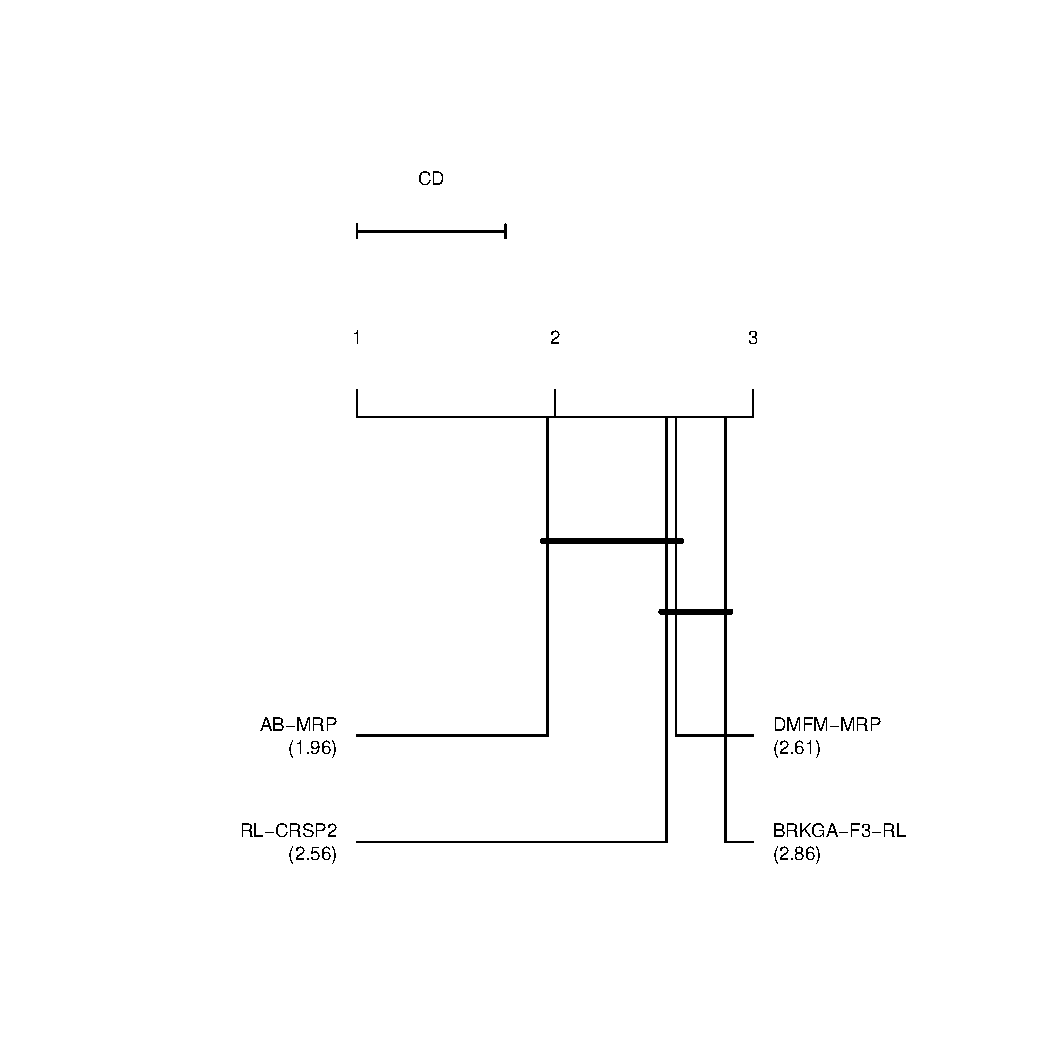
\includegraphics[scale=0.6]{imagens/ls_all.pdf}
        \vspace*{-2cm}
        \caption{ID = 3.73, VC = 2.68, DC = 0.74}
    \end{subfigure}
    \caption{Testes de Iman-Davenport e Nemenyi para os Limitantes Superiores.}
    \label{fig:all-ls-nemenyi}
\end{figure}

O  modelo  \gls{ab-pma}  obteve  o   melhor  desempenho  dentre  as  abordagens,
garantindo  \gls{ls}s  melhores  ou  iguais   às  demais  metodologias  para  37
instâncias do conjunto. Mais especificamente, em 8 instâncias o valor obtido foi
melhor dentre  todos os algoritmos.  Considerando o modelo  \gls{dmfm-pma}, cujo
valor de {\em  rank} médio está bem  próximo ao {\em rank}  da relaxação {\rlq},
observa-se que  a contagem de  vitórias entre eles  foi idêntica, 11  casos para
cada um. Por fim, temos os resultados da versão do \gls{brkga} F3-RL, que obteve
limitantes iguais aos melhores obtidos pelas demais abordagens em 18 instâncias,
mas que, ainda assim, manteve-se no pior \textit{rank} médio.



\chapter{Considerações Finais} \label{chp:consideracoes-finais}

Os objetivos principais deste trabalho  consistiram na definição e realização de
um estudo  computacional do \gls{pma}  conduzido a partir  de um conjunto  de 40
instâncias baseadas em simulação de tráfego e de rede. Foram exploradas técnicas
de  solução  exata utilizando  \gls{pli}  e  Relaxações Lagrangianas  e  métodos
heurísticos capazes de gerar limitantes inferiores e superiores.

Considerando os métodos exatos, foram adaptados pré-processamentos, apresentados
por   Ribeiro   et   al.   \cite{tiago:2019},   para   fixação   de   variáveis.
Desenvolveram-se dois modelos matemáticos,  \gls{dmfm-pma} e \gls{ab-pma}. Ambos
se mostraram eficazes em resolver de maneira  ótima instâncias com até 125 nós e
gerando  soluções viáveis  para todas  as 40  instâncias do  conjunto de  teste.
Ainda, o  \gls{dmfm-pma} serviu de  base para  o desenvolvimento de  um conjunto
contendo quatro Relaxações Lagrangianas (\gls{rl}). Tais relaxações apresentaram
bons resultados com baixo consumo de  tempo, fato que permite a possibilidade de
utilização para instâncias maiores.

Em relação  aos métodos  heurísticos, foi desenvolvida  uma heurística  de busca
local  em arborescências,  aplicada conjuntamente  ao algoritmo  de solução  das
\gls{rl}s, objetivando  a geração  e aperfeiçoamento  de soluções  viáveis. Além
disso, foram  desenvolvidas quatro variações da  meta-heurística \gls{brkga}, de
modo que  três delas  variam a  função de  aptidão do  decodificador e  a última
abordagem extrai a frequência de arcos durante a resolução da \gls{rl} e utiliza
essa informação na geração das chaves aleatórias.

Ao final,  todos os algoritmos  foram comparados através de  testes estatísticos
não  paramétricos. Como  não existem  resultados para  o \gls{pma}  presentes na
literatura,  destaca-se  a necessidade  da  comparação  de resultados  entre  as
diferentes  metodologias  desenvolvidas.  De   tal  modo,  é  possível  validar,
utilizando  múltiplas  abordagens,  a  qualidade  dos  limitantes  inferiores  e
superiores. Ao  considerar o  conjunto de  todas as  metodologias desenvolvidas,
destaca-se  o modelo  \gls{ab-pma}  como  a melhor  abordagem  para obtenção  de
\gls{li}s  e  \gls{ls}s.  As  \gls{rl}s   geram  bons  limitantes  inferiores  e
superiores, não sendo melhores que os modelos para todos os casos, mas o fato de
existirem  versões combinatórias  eficientes,  permite a  solução de  instâncias
maiores.  Por fim,  mesmo  testando  diversas funções  de  aptidão e  detectando
melhoras com  a alteração do processo  de geração de chaves  aleatórias, não foi
possível  gerar \gls{ls}s  com o  \gls{brkga}  que estivessem  acima das  demais
abordagens desenvolvidas.

Como  trabalhos futuros,  pode-se destacar  o possibilidade  de tornar  o modelo
\gls{ab-pma} mais  forte, por  exemplo considerando  um conjunto  exponencial de
restrições para garantir conectividade entre nós.  Por ser de aplicação geral em
arborescências, a  heurística de busca  local desenvolvida pode ser  aplicada em
outras  meta-heurísticas.  Ainda, pode-se  expandir  o  conjunto de  instâncias,
tratando de simulações  cada vez maiores em quantidade de  veículos ou até mesmo
considerando dados que se baseiam em cenários reais.

As técnicas desenvolvidas neste trabalho podem ser aplicadas em outras variantes
do \gls{pma} como \gls{mrp-qos} considerando  as mesmas métricas de \gls{qos} ou
adicionando  mais restrições  ao conjunto,  tais  como o  número de  saltos e  a
estimativa de  duração do enlace. Ainda  é possível gerar resultados  para novas
variantes que  combinam o  \gls{pma} com  o \gls{mrp-qos},  ou seja,  o objetivo
consiste em decidir quais terminais serão  atendidos e ao mesmo tempo computar o
caminho de menor custo no atendimento desse terminal.




% a frequência dos arcos da utilizados
% na relaxação lagrangiana como um viés aplicado às chaves aleatórias geradas.
% ,  de  modo  que  o  primeiro  deles
% (denotado  por \gls{dmfm-pma})  consegue  encontrar soluções  ótimas para  quase
% todas as  instâncias de até 100  nós no tempo máximo  de uma hora e  serviu como
% base  para   o  desenvolvimento   de  um   conjunto  de   diferentes  relaxações
% lagrangianas.  O segundo  modelo  (denotado por  \gls{ab-pma}),  sendo a  última
% abordagem desenvolvida nesta dissertação,  conseguiu gerar soluções viáveis para
% todas as 40 instâncias do conjunto, obtendo dentre elas 28 soluções ótimas. Além
% disso,  ambos modelos  obtiveram o  melhor desempenho  na geração  de limitantes
% inferiores  e o  modelo \gls{ab-pma}  se mostrou  a metodologia  mais eficaz  na
% geração de limitantes superiores.


% As referências:
\bibliographystyle{plain}
\bibliography{ic-tese-v3}


% Os anexos, se houver, vêm depois das referências:
%\appendix
%\chapter{Anexo 1}
%\chapter{Anexo 2}

\end{document}
